% -*- Mode:TeX -*-

%% IMPORTANT: The official thesis specifications are available at:
%%            http://libraries.mit.edu/archives/thesis-specs/
%%
%%            Please verify your thesis' formatting and copyright
%%            assignment before submission. If you notice any
%%            discrepancies between these templates and the 
%%            MIT Libraries' specs, please let us know
%%            by e-mailing thesis@mit.edu

%% The documentclass options along with the pagestyle can be used to generate
%% a technical report, a draft copy, or a regular thesis. You may need to
%% re-specify the pagestyle after you \include cover.tex. For more
%% information, see the first few lines of mitthesis.cls. 

%\documentclass[12pt,vi,twoside]{mitthesis}
%%
%%  If you want your thesis copyright to you instead of MIT, use the
%%  ``vi'' option, as above.
%%
%\documentclass[12pt,twoside,leftblank]{mitthesis}
%%
%% If you want blank pages before new chapters to be labelled ``This
%% Page Intentionally Left Blank'', use the ``leftblank'' option, as
%% above. 

\documentclass[12pt,twoside]{mitthesis}
\usepackage{lgrind}
%% These have been added at the request of the MIT Libraries, because
%% some PDF conversions mess up the ligatures.  -LB, 1/22/2014
\usepackage{cmap}
\usepackage[T1]{fontenc}
\pagestyle{plain}

%% This bit allows you to either specify only the files which you wish to
%% process, or `all' to process all files which you \include.
%% Krishna Sethuraman (1990).

%\typein [\files]{Enter file names to process, (chap1,chap2 ...), or `all' to process all files:}
\def\all{all}
\ifx\files\all \typeout{Including all files.} \else %\typeout{Including only \files.} \includeonly{\files} \fi

\begin{document}

% -*-latex-*-
% 
% For questions, comments, concerns or complaints:
% thesis@mit.edu
% 
%
% $Log: cover.tex,v $
% Revision 1.9  2019/08/06 14:18:15  cmalin
% Replaced sample content with non-specific text.
%
% Revision 1.8  2008/05/13 15:02:15  jdreed
% Degree month is June, not May.  Added note about prevdegrees.
% Arthur Smith's title updated
%
% Revision 1.7  2001/02/08 18:53:16  boojum
% changed some \newpages to \cleardoublepages
%
% Revision 1.6  1999/10/21 14:49:31  boojum
% changed comment referring to documentstyle
%
% Revision 1.5  1999/10/21 14:39:04  boojum
% *** empty log message ***
%
% Revision 1.4  1997/04/18  17:54:10  othomas
% added page numbers on abstract and cover, and made 1 abstract
% page the default rather than 2.  (anne hunter tells me this
% is the new institute standard.)
%
% Revision 1.4  1997/04/18  17:54:10  othomas
% added page numbers on abstract and cover, and made 1 abstract
% page the default rather than 2.  (anne hunter tells me this
% is the new institute standard.)
%
% Revision 1.3  93/05/17  17:06:29  starflt
% Added acknowledgements section (suggested by tompalka)
% 
% Revision 1.2  92/04/22  13:13:13  epeisach
% Fixes for 1991 course 6 requirements
% Phrase "and to grant others the right to do so" has been added to 
% permission clause
% Second copy of abstract is not counted as separate pages so numbering works
% out
% 
% Revision 1.1  92/04/22  13:08:20  epeisach

% NOTE:
% These templates make an effort to conform to the MIT Thesis specifications,
% however the specifications can change. We recommend that you verify the
% layout of your title page with your thesis advisor and/or the MIT 
% Libraries before printing your final copy.
\title{Hand detection, segmentation and tracking from egocentric vision}

\author{Van-Tien Pham}
% If you wish to list your previous degrees on the cover page, use the 
% previous degrees command:
%       \prevdegrees{A.A., Harvard University (1985)}
% You can use the \\ command to list multiple previous degrees
%       \prevdegrees{B.S., University of California (1978) \\
%                    S.M., Massachusetts Institute of Technology (1981)}
\department{School of Information Technology and Communication}

% If the thesis is for two degrees simultaneously, list them both
% separated by \and like this:
% \degree{Doctor of Philosophy \and Master of Science}
\degree{Master of Science in Information System and Communication}

% As of the 2007-08 academic year, valid degree months are September, 
% February, or June.  The default is June.
\degreemonth{October}
\degreeyear{2020}
\thesisdate{October 10, 2020}

%% By default, the thesis will be copyrighted to MIT.  If you need to copyright
%% the thesis to yourself, just specify the `vi' documentclass option.  If for
%% some reason you want to exactly specify the copyright notice text, you can
%% use the \copyrightnoticetext command.  
%\copyrightnoticetext{\copyright IBM, 1990.  Do not open till Xmas.}

% If there is more than one supervisor, use the \supervisor command
% once for each.
\supervisor{Thi-Thanh-Hai Tran}{Associate Professor}

% This is the department committee chairman, not the thesis committee
% chairman.  You should replace this with your Department's Committee
% Chairman.
\chairman{Chairman}{Chairman, Department Committee on Graduate Theses}

% Make the titlepage based on the above information.  If you need
% something special and can't use the standard form, you can specify
% the exact text of the titlepage yourself.  Put it in a titlepage
% environment and leave blank lines where you want vertical space.
% The spaces will be adjusted to fill the entire page.  The dotted
% lines for the signatures are made with the \signature command.
\maketitle

% The abstractpage environment sets up everything on the page except
% the text itself.  The title and other header material are put at the
% top of the page, and the supervisors are listed at the bottom.  A
% new page is begun both before and after.  Of course, an abstract may
% be more than one page itself.  If you need more control over the
% format of the page, you can use the abstract environment, which puts
% the word "Abstract" at the beginning and single spaces its text.

%% You can either \input (*not* \include) your abstract file, or you can put
%% the text of the abstract directly between the \begin{abstractpage} and
%% \end{abstractpage} commands.

% First copy: start a new page, and save the page number.
%\cleardoublepage
% Uncomment the next line if you do NOT want a page number on your
% abstract and acknowledgments pages.
\pagestyle{empty}
\setcounter{savepage}{\thepage}
\begin{abstractpage}
% $Log: abstract.tex,v $
% Revision 1.1  93/05/14  14:56:25  starflt
% Initial revision
% 
% Revision 1.1  90/05/04  10:41:01  lwvanels
% Initial revision
% 
%
%% The text of your abstract and nothing else (other than comments) goes here.
%% It will be single-spaced and the rest of the text that is supposed to go on
%% the abstract page will be generated by the abstractpage environment.  This
%% file should be \input (not \include 'd) from cover.tex.
Multiple object tracking is the process of assigning unique and consistent identities to objects throughout a video sequence. A de-facto approach to multiple object tracking, and object tracking in general, is to use a method called tracking by detection. Tracking by detection is a two-stage procedure: an object detection or segmentation algorithm fist detects objects in a given frame, these detected objects are then associated with already tracked objects in a second step by a tracking algorithm. Egocentric vision is an emerging field of computer vision that is characterized by the acquisition of images and video from the first-person perspective. In egocentric view, the two human hands are essential in the execution of actions and characterizing their movements and trajectories are the principal cues to define and recognize actions.
\\One of the main concerns of this thesis is to develop an automatic tracking by detection algorithm that extracts hands positions and identities in consequence frames from egocentric surveillance video. The proposed framework consists of state-of-the-art detectors from RCNN and YOLO family models combined with the SORT or DeepSORT for object tracking task. The thesis aims to explore how the stand-alone alone performance of the object detection algorithm correlates with overall performance of a tracking-by-detection system. Finally, the thesis investigates how the use of visual descriptors of DeepSORT in the tracking stage of a tracking-by-detection system effects performance.
\\Results presented in this thesis suggest that the capacity of the object detection algorithm is highly indicative of the overall performance of the tracking-by detection system. Further, this thesis also shows how the use of visual descriptors in the tracking stage can reduce the number of identity switches and thereby increase performance of the whole system. This thesis also presents a new egocentric hand tracking dataset Micand32 for future researches.


\end{abstractpage}

% Additional copy: start a new page, and reset the page number.  This way,
% the second copy of the abstract is not counted as separate pages.
% Uncomment the next 6 lines if you need two copies of the abstract
% page.
% \setcounter{page}{\thesavepage}
% \begin{abstractpage}
% % $Log: abstract.tex,v $
% Revision 1.1  93/05/14  14:56:25  starflt
% Initial revision
% 
% Revision 1.1  90/05/04  10:41:01  lwvanels
% Initial revision
% 
%
%% The text of your abstract and nothing else (other than comments) goes here.
%% It will be single-spaced and the rest of the text that is supposed to go on
%% the abstract page will be generated by the abstractpage environment.  This
%% file should be \input (not \include 'd) from cover.tex.
Multiple object tracking is the process of assigning unique and consistent identities to objects throughout a video sequence. A de-facto approach to multiple object tracking, and object tracking in general, is to use a method called tracking by detection. Tracking by detection is a two-stage procedure: an object detection or segmentation algorithm fist detects objects in a given frame, these detected objects are then associated with already tracked objects in a second step by a tracking algorithm. Egocentric vision is an emerging field of computer vision that is characterized by the acquisition of images and video from the first-person perspective. In egocentric view, the two human hands are essential in the execution of actions and characterizing their movements and trajectories are the principal cues to define and recognize actions.
\\One of the main concerns of this thesis is to develop an automatic tracking by detection algorithm that extracts hands positions and identities in consequence frames from egocentric surveillance video. The proposed framework consists of state-of-the-art detectors from RCNN and YOLO family models combined with the SORT or DeepSORT for object tracking task. The thesis aims to explore how the stand-alone alone performance of the object detection algorithm correlates with overall performance of a tracking-by-detection system. Finally, the thesis investigates how the use of visual descriptors of DeepSORT in the tracking stage of a tracking-by-detection system effects performance.
\\Results presented in this thesis suggest that the capacity of the object detection algorithm is highly indicative of the overall performance of the tracking-by detection system. Further, this thesis also shows how the use of visual descriptors in the tracking stage can reduce the number of identity switches and thereby increase performance of the whole system. This thesis also presents a new egocentric hand tracking dataset Micand32 for future researches.


% \end{abstractpage}

%\cleardoublepage

\section*{Acknowledgments}

First of all, I might want to offer my special thanks to my supervisor, Assoc. Prof. Tran Thi Thanh Hai. I'd really appreciate everything she've guided me all through this thesis.

I would like to thank my colleagues at Viettel High Technology Industries Corporation for supporting me in technical issues. Also, I might want to express gratitude toward Assoc. Prof. Vu Hai and alumni at MICA Institute, Hanoi University of Science and Technology for giving me significant suggestions.

Deep inside my heart, I wish to show my gratefulness to my family for always inspiring and trusting me in every of my steps.

%%%%%%%%%%%%%%%%%%%%%%%%%%%%%%%%%%%%%%%%%%%%%%%%%%%%%%%%%%%%%%%%%%%%%%
% -*-latex-*-


% Some departments (e.g. 5) require an additional signature page.  See
% signature.tex for more information and uncomment the following line if
% applicable.
% % -*- Mode:TeX -*-
%
% Some departments (e.g. Chemistry) require an additional cover page
% with signatures of the thesis committee.  Please check with your
% thesis advisor or other appropriate person to determine if such a 
% page is required for your thesis.  
%
% If you choose not to use the "titlepage" environment, a \newpage
% commands, and several \vspace{\fill} commands may be necessary to
% achieve the required spacing.  The \signature command is defined in
% the "mitthesis" class
%
% The following sample appears courtesy of Ben Kaduk <kaduk@mit.edu> and
% was used in his June 2012 doctoral thesis in Chemistry. 

\begin{titlepage}
\begin{large}
This doctoral thesis has been examined by a Committee of the Department
of Chemistry as follows:

\signature{Professor Jianshu Cao}{Chairman, Thesis Committee \\
   Professor of Chemistry}

\signature{Professor Troy Van Voorhis}{Thesis Supervisor \\
   Associate Professor of Chemistry}

\signature{Professor Robert W. Field}{Member, Thesis Committee \\
   Haslam and Dewey Professor of Chemistry}
\end{large}
\end{titlepage}



\pagestyle{plain}
  % -*- Mode:TeX -*-
%% This file simply contains the commands that actually generate the table of
%% contents and lists of figures and tables.  You can omit any or all of
%% these files by simply taking out the appropriate command.  For more
%% information on these files, see appendix C.3.3 of the LaTeX manual. 
\tableofcontents
%\newpage
\listoffigures
%\newpage
\listoftables



\chapter{Introduction}\label{chap:intro}

\section{Overview of object recognition and tracking from video}
\subsection{Object recognition}
Object recognition aims at detecting the presence of an object in image and giving it a label that is the category to which it belongs. Objects of interest can be face, vehicle, hand, people, tree, tumors depending on applications such as face id, intelligent traffic system and autonomous vehicles, human machine interaction, health care, security or bio diversity, etc. Segmentation is fundamental that go further than object detection and classification by give a label to a pixel, not a bounding box. There are two types of segmentation: semantic segmentation and instance segmentation. Semantic segmentation classifies all pixels of an image into meaningful object categories. These categories are "semantically interpretable" and correspond to the classes in the real world. Semantic segmentation gives an unique label to two objects of the same category. This is called dense prediction because it can predict the meaning of each pixel. Instance segmentation otherwise gives every pixel belonging to an object instance a label.
Since the past decade, object detection and recognition as well as segmentation has achieved impressive performance thanks to the significant advances of AI and deep learning. Deep learning can learn patterns in visual input in order to predict not only the categories of objects in image but also the ones of pixels. Deep learning architectures used for object detection / recognition / segmentation are convolutional neural networks (CNN) or specific CNN frameworks such as AlexNet, VGG, Inception and ResNet.
\subsection{Object tracking}
Tracking objects in a video stream involves association of moving objects in consecutive video frames. In order to track an object, the target object requires to be firstly detected manually (detection free trackers) or automatically by detection algorithms (detection based tracker). Then tracking algorithm will associate detected objects to existing tracks by putting constraints on distance function between movement and appearance of the object with its previous instances.  Besides giving a complete trajectory of a moving object during time that are very important for video analysis. Tracking is more helpful to solve some common challenges (e.g. as lighting changes, motion blur, zoom ratio changes, occlusion when the target is partially or completely hidden by another object in the video for a period of time, poor image quality) from that simple object detection often suffers from.
\\Almost proposed trackers until now based on Siamese network or Correlation Filter (CF), combined with effective appearance models (CNN function, HOG, color name). In challenges on object tracking task, most of the highest performance obtained with CF trackers. Their performances is better than Siam tracker. In term of computational time, Siam tracker's performance is better than CF. Depending on the context and application, tracking could be single object tracking (SOT) and multiple object tracking (MOT).
MOT is more challenging than SOT because ID switching is difficult to avoid, especially in crowded videos, the nature and number of objects in each frame are unknown. Therefore, MOT algorithms strongly rely on detection algorithms. Unfortunately, detection algorithms itself are not perfect. A popular object tracking method is to use a method called tracking by detection. It first apply object detection algorithms to detect objects in current frame. These objects are then tracked by associating the objects in the current frame with the objects in the previous frame using a tracking algorithm. Having a reliable object detection method is crucial, because the tracking algorithm depends on the objects detected in each frame. Recently, target detection algorithms based on convolutional neural networks have been able to achieve higher accuracy than traditional target detection methods. The improvement of object detection accuracy promotes the use of one-by-one detection and tracking method for multiple object tracking.
\section{Context and scope of the thesis}
\subsection{Egocentric vision}
Egocentric vision or first-person vision (FPV) is a subfield of computer vision, which requires the analysis of images and videos captured by a wearable camera, which is usually worn on the head or chest, and naturally approximates the camera wearer vision. Therefore, the visual data captures the part of the scene where the user is focused on performing on-site tasks and provides a valuable perspective to understand the user's activities and their environment in the natural environment.
In recent years, the research community has adopted a self-centered perspective to solve computer vision challenges, such as activity recognition \cite{10.1109/ICCV.2011.6126269} and object detection \cite{5995444} that are traditionally considered to belong to the field of third-person vision. Since then, self-centered vision has been applied to more complex applications, including video summarization \cite{6247820} and social interaction analysis \cite{7780657}. It is worth noting that it has also been extended to the field of healthcare \cite{wearable}, in which static camera systems tend to struggle to a greater degree with regard to privacy issues \cite{6091176}. Ultimately, self-centered vision is associated with the field of augmented reality to enhance human-centered applications that provide help for specific tasks \cite{10.1145/3041164.3041185}, thereby enhancing human independence; applicable to human capabilities Damaged or reduced condition.
In the medical field, FPV can help to build applications that aid people with dementia by recording the sensor carrier's day-to-day activities. In rehabilitation therapy, or motor support in the elderly, physicians are often interested in monitoring the patient's recovery progress through movements and daily activities such as arm lifts, move the wrist in the grasp object. Currently, monitoring are mainly using the naked eye for observation, automatic monitoring tools are very limited in hospitals. Through the automatic analysis and recognition of activities from the series of images captured by the carrier camera (FPV video), the treating doctor can identify and quantify the patient's progression for a therapeutic regimen value accordingly.
In sports, the use of egocentric cameras is increasingly common. The egocentric systems don't just collect front-view imagery during the journey of speed sports such as cycling and skiing; but also supports analysis of accuracy in sports movements such as golf, basketball. One notable feature is that the FPV image sequence not only contains information about the ego-motion of the object itself, but also the interactive movements between the hand and the subject (shadow, golf club) simultaneously. In sports, the recording of movements at critical moments (ball contact point, hand movement direction) plays an important role in determining the athlete's success or failure.
In the field of teaching aids, virtual reality, the use of FPV techniques has brought remarkable results. It can be considered the role of the camera carried on the body as a sixth sense (six-sense). On the one hand, FPV assists in detecting the behavior (e.g. hand gestures) of the subject, on the other hand, the camera carries the observer or the affected person. From there, the system reacts in accordance with the user's requirements. One particular application is the interaction between an observed object and the person carrying a sensor while visiting a museum; The system can on the one hand detect the object that the visitor is interested in, on the other hand identify the behavior (gesture) that the visitor wants to interact with the system (to support details, or see objects from different perspectives). In educational applications, virtual reality is receiving more and more attention besides medical applications when developing Ego-centric vision systems.
\subsection{Background project and motivation}
This thesis falls under the scope of the project “Understanding Human Daily Life Activities from Egocentric Vision Using Advanced Technologies of Deep Learning” funded by National Foundation for Science and Technology Development (NAFOSTED). The objective of this project is to analyze activities of human (elderly people or patients) in daily life or during rehabilitation through analyzing two important factors: the role of hand gestures in interacting with objects; and the role of the environment in identifying sensor carrier activity.
To achieve these goals, the project focuses on solving the fundamental problems of egocentric-vision such as: summarizing video from large data sources (up to millions of images/day), effectively exploiting relationships between the sensor carrier and the interactive object/object; and environment/context. Specifically, the project implements three main tasks: (1) developing advanced deep learning techniques for hand segmentation and activities recognition, (2) exploiting the correlation between different factors such as  environment condition, time execution and the way of execution of a certain exercise/activity; (3) deploying proposed techniques to evaluate the rehabilitation of patients after a period of training.
\\My thesis in the project focuses on detecting, segmenting and tracking human hand in egocentric videos. I first study existing deep learning based methods for object segmentation and tracking then propose a framework that takes consecutive frames as input, segments hand regions frame by frame then does hand tracking along frames. I then implement the framework which allows to flexibly integrate different CNN architectures for objects detection (i.e. YOLO \cite{DBLP:journals/corr/RedmonDGF15}, Faster CNN \cite{DBLP:journals/corr/RenHG015}, Mask R-CNN \cite{DBLP:journals/corr/HeGDG17}) as well as object tracking (i.e. SORT \cite{DBLP:journals/corr/BewleyGORU16}, DeepSORT \cite{DBLP:journals/corr/WojkeBP17}). To train CNN models, I develop a tool to speed up the tracking annotation using automatic segmentation results. Finally, I evaluate the developed framework on the a hand dataset captured in the context of the project.
\section{Related works}
\subsection{Video object recognition and tracking challenges}
Densely Annotated Video Segmentation (DAVIS) challenge \cite{7780657} is a fairly famous public competition designed for the task of video object segmentation that has been going on for 4 years from 2016 to 2020. It is a benchmark dataset and evaluation methodology for video object segmentation that consists of fifty high quality, full HD video sequences, accompanied by densely annotated, pixel-accurate and per-frame ground truth segmentation. It provides a comprehensive analysis of several state-of-the-art segmentation approaches using three complementary metrics. These are: semi-supervised challenge, interactive challenge and unsupervised challenge with specific datasets, definitions, rules and evaluation metrics.
The popular Visual Object Tracking (VOT) challenges \cite{VOT_TPAMI} provides the visual tracking community with a precisely defined and repeatable way to compare short-term trackers, and provides a common platform for discussing evaluation and progress in the field of visual tracking. The goal of the challenge is to build a large database of benchmarks and organize seminars or similar activities to promote research on visual tracking.
Multiple Object Tracking (MOT) \cite{DBLP:journals/corr/MilanL0RS16} challenge is a well-known benchmark for multi-object tracking that collects a large variety of sequences and provides a framework for the standardized evaluation of multiple object tracking methods. Currently, the benchmark is focused on multiple people tracking, since pedestrians are by far the most studied object in the tracking community. The benchmark includes 2D, 3D and multi-camera challenges. The tracking evaluation is this thesis uses the devkit protocol of the MOT16 which provide several measures, from recall to precision to running time. 
\subsection{Hand gestures recognition related works}
One of the first works on the understanding of egocentric activities focused on defining the inner message of the egocentric visual paradigm \cite{10.1109/ICCV.2011.6126269}. They use the extracted visual features to model the relationship between hands, objects, and actions to model activities, and demonstrate the mutual improvement provided by these relationships through bottom-up and top-down models.
In \cite{5995444}, the authors have developed a weakly supervised technique that can identify objects by sculpting out objects from large sequences of self-centered activities. In general, this is a difficult task, their algorithm uses domain-specific knowledge from a first-person perspective to make it feasible. The method will automatically segment the active object area, assign some areas to each object, and use semi-supervised learning to disseminate its information. They proved that this method can reliably compare active classes based on the usage patterns of objects.

Movement-based egocentric action recognition is described in \cite{7298625}. According to the motion and color-based features and trajectories extracted from the video frames, the interaction points of the hand and the object, the object, the head and the self-movement are declared as actions, but the position of the modeled hand is not paid special attention. \cite{7780578} describes another multi-modal approach to egocentric activity recognition. Here, the hand segmentation network, the object localization network and the network trained by the motion flow are combined to predict the action.

In \cite{DBLP:journals/corr/BertasiusPYS16}, an architecture based on two-stream visual segmentation was used to predict the interaction area between hands and objects in a video stream and model them as actions. In \cite{cai2016understanding}, the concept of hand-object interaction is further explored, and the object shape-related grasping related to modeling actions is detected. The end-to-end approach also includes \cite{DBLP:journals/corr/abs-1806-06157}, where in order to recognize actions, the network is trained on paired frames and optimized for action recognition, object segmentation and inter-frame object interaction, as well as their training targets associated with recurrent networks. This work also assumes that hands and objects are the basis of self-centered actions, but it emphasizes the need to clearly detect the areas and positions of hands and objects to recognize actions.
A lot of works have been done in the explicit exploration of opponents and objects and their temporal relationships. Hand detection, segmentation and recognition techniques were developed \cite{6619302} \cite{6910041} \cite{10.1016/j.cviu.2016.09.005}, and the results were used to model behaviors or activities. In \cite{7410583}, hand-based activity recognition from an egocentric perspective is discussed. Before inferring the activity, the EgoHands dataset and the egocentric hand detection and segmentation pipeline were developed. This is one of the manual works, showing the difference between relying on hand detection or segmentation and using manual label for activity classification. In the literature \cite{Recognition}, activity recognition based on egocentric hands is considered, in which the distance between the detected hands or the distance between the detected hands and the objects marked as activities is considered as the feature of activity classification.
In \cite{9060114}, the egocentric human action recognition is solved by explicitly using the existence and location of the region of interest in the scene without further use of visual features. Their understanding that the human hand is very important in performing actions, and focused on its actions as the main clues to define actions. Finally, in all the works above, the suggestion on the choice of a suitable methods for online tracking applications is unavailable.
\section{Problem formulation and assumptions}
\subsection{Objective}
\begin{table}
	\caption{Problem formulation.}
	\label{formulation}
	\begin{tabular}{|l|p{13cm}|}
		
		\hline 
		Input &  Sequence of frames from an egocentric surveillance video\\ 
		\hline 
		Output & Trajectories of the tracked hands, includes: \\
		& \tabitem The number of human hands in the current frame \\
		& \tabitem The location of each hand, represented by a bounding box for the detection algorithm, or a set of pixels for the segmentation algorithm \\
		& \tabitem Identity of each hand across the video
\\ 
		\hline 
	\end{tabular}
\end{table}
Table \ref{formulation} defines the input and output of the problem in this thesis. The goal of this thesis is to solve the problem of detecting, segmenting and tracking human hand objects in the video from the first perspective. Along with researching, confirming the theory, and proposing a hand tracking by detection system, I built a module to detect and track human hands in videos from the first perspective. The tracking by detection approach uses the combination of a detector and a tracker as following:
\begin{itemize}
	\item Detector: Faster RCNN, Mask RCNN, MaskRCNN with region based, YOLOv3, YOLOv4 or Ground-truth
	\item Tracker: SORT or DeepSORT
\end{itemize}
The inference results on test dataset are used to analyze the effect of phase detection algorithm selection on hand tracking phase, and also the efficiency of the DeepSORT algorithm compared to the SORT algorithm in the tracking phase.
\subsection{Contribution}
The main contributions of this thesis are three-folds:
\begin{itemize}
	\item First, a framework for hand detection, segmentation and tracking from egocentric vision pipeline is proposed. This framework contains state-of-the-art detection algorithms in RCNN and YOLO families for object detection and segmentation, and two tracking algorithm SORT and DeepSORT for object tracking. Any other algorithms can be simply integrated into this framework.
	\item Second, a comparative evaluation of combination of a detector and a tracker is conducted and analyzed on both term of accuracy and performance. Consequently, the recommendation for choosing a suitable method for egocentric hand tracking applications is given.
	\item Third, Micand32, a new egocentric hand detection, segmentation and tracking datasets is built during this thesis, accompanied with labeling, visualizing and evaluation tools.
\end{itemize}
A part of this thesis is published in the Proceeding of the \(3^{rd}\) International Conference on Multimedia Analysis and Pattern Recognition \cite{tien}. The code developed in this thesis will made available at \faicon{github} \url{https://github.com/pvtien96/Detectron2DeepSortPlus}.
\subsection{Thesis outline}
The thesis is structured into 5 chapters:
\begin{enumerate}
	\item \textbf{Introduction} summarize the overview of object recognition, including object classification, detection, segmentation and tracking in the wild and in the first persion vision (FPV). Related works are studied and dicussed. The thesis's scope, objective and contribution are then described.
	\item \textbf{Methodology and Datasets} presents the RCNN and YOLO family models; SORT and DeepSORT algorithms. This chapter analyse egocentric hand datasets incoporate GTEA family, EgoHand; and futhermore present a new egocentric hand tracking datasets Micand32 alongside with a semi-automatic annotator,the EHTA.
	\item \textbf{Proposed Framework} introduces the proposed architecture which contains 4 stage: data preparing stage, training stage, inference stage and evaluation stage. This chapter reports in detail techniques in training and tesing phase.
	\item \textbf{Experiments} conserves about the evaluation criteria and then enumerate overall and featured detection, segmentation result following the COCO dataset standard and tracking result of 11 aproaches on Micand32S and Micand32E following the MOT Challenge standard. 
	\item \textbf{Conclusion} terminates the thesis by considering the accomplishment, the drawback and also purpose some potential future works.
\end{enumerate}
%% This is an example first chapter.  You should put chapter/appendix that you
%% write into a separate file, and add a line \include{yourfilename} to
%% main.tex, where `yourfilename.tex' is the name of the chapter/appendix file.
%% You can process specific files by typing their names in at the 
%% \files=
%% prompt when you run the file main.tex through LaTeX.
\chapter{Methodology and Datasets}\label{chap:method}
\section{Tracking by detection approach}
Tracking multiple objects is a task of assigning an unique and consistent identifier to each object in a video series. This section presents an object tracking technique called "tracking by detection". Tracking through detection is a two-stage process: the object detection algorithm first detects the objects present in the frame. These detected objects are then linked to those that have been tracked through a tracking algorithm. Usually, the object detection algorithm and tracking algorithm are completely separate from each other, so they can be analyzed separately.
Object detection is a process of detecting specific categories of objects in an image, examples of these categories are things such as pedestrian or car. The purpose of the object detection algorithm is to locate and classify objects belonging to any popular category. Therefore, for each detected object, the object detection algorithm produces an estimate of the object's location, size, and category. The position and size of the detected object are usually represented by a bounding box, which is a rectangular box surrounding the object. The range of the detected object can also be defined by a segmentation mask, which is a pixel-level mask of the object.
Due to recent advances in the field of image classification, target detection has made considerable progress. This progress is attributed to a breakthrough in how to use CNN for image classification \cite{10.1145/3065386}. The target detection algorithm usually consists of a CNN designed for image classification, and then has an algorithm-specific additional structure around the CNN. CNN is called the backbone of the algorithm, and the algorithm-specific structure is called the meta-architecture. By convention, in this thesis, I identify object detection algorithm through its meta-architecture. CNN-based object detection algorithm can be divided into two different groups: single-stage and two-stage detectors \cite{DBLP:journals/corr/abs-1808-07256}. The two-stage detector first generates bounding boxes by segmenting the image into regions of interest, and then CNN classifies these regions in the second stage. The single-stage detector is bounding box and class estimates in a single forward pass of the image through the CNN. Traditionally, two-stage detectors have achieved higher accuracy at the expense of speed compared to single-stage detectors. However, the recently introduced loss function Focal loss \cite{DBLP:journals/corr/abs-1708-02002} makes the accuracy of a single-stage detector close to that of a two-stage detector. The trade-off between speed and accuracy is the main design choice, as studied in the paper \cite{DBLP:journals/corr/HuangRSZKFFWSG016}.
The tracking algorithm in the "tracking by detection" framework is responsible for assigning unique identifiers to the tracked objects and establishing object associations between frames. In my work, I focuses on target detection algorithm, and particularly considers two different tracking algorithm: SORT and DeepSORT SORT stands for simple online and real-time tracking. It is a deliberately simple tracking algorithm that uses a Kalman filter \cite{10.1115/1.3662552} to estimate the future position of an object, and uses the Hungarian method \cite{doi:10.1002/nav.3800020109} for frame-to-frame correlation. Deep SORT is an extension of SORT that incorporates appearance information when performing object association between frames.
\section{Object detection and segmentation algorithms}
\subsection{RCNN model}
\subsubsection{RCNN}
R-CNN is an abbreviation for regions with CNN features, and is an object detection method introduced by Girschick et al in \cite{DBLP:journals/corr/GirshickDDM13}. The system consists of three main components: region proposal, convolutional neural network and a set of support vector machines (SVM).
Figure \ref{fig:rcnnSche} shows the relation of R-CNN's component. First, the region proposal method divides the image into regions irrelevant to the category. Each image produces approximately 2000 regions. After segmenting the image, each region is deformed into a fixed size to fit the required input size of the CNN. Next, feed 2000 deformed regions through CNN, and extract feature vectors for each region. Then, the feature vectors are registered by a set of linear SVMs, where each SVM is trained to classify a specific category. Finally, given the class predicted by SVM, regression is used to improve the predicted shape of the bounding box. Given a predicted bounding box coordinate \(p=(p_x,p_y,p_w,p_h)\) (center coordinate, width, height) and its corresponding ground truth box coordinates \(g=(g_x,g_y,g_w,g_h )\), the regressor is configured to learn scale-invariant transformation between two centers and log-scale transformation between widths and heights. All the transformation functions take p as input.
\begin{equation}
	\hat g_x=p_w d_x (p)+p_x
\end{equation}
\begin{equation}
	\hat g_y=p_h d_x (p)+p_y
\end{equation}
\begin{equation}
	\hat g_w=p_w \exp{(d_w(p))}
\end{equation}
\begin{equation}
	\hat g_h=p_h \exp{(d_h(p))}
\end{equation}
%\begin{figure}
%	\centerline{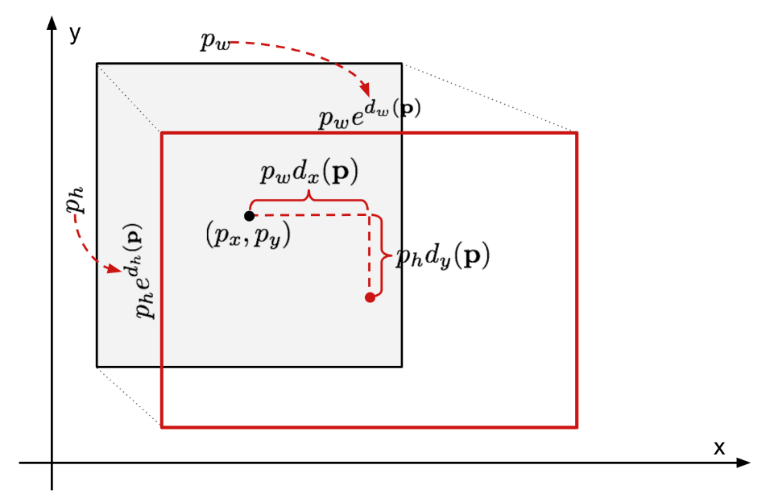
\includegraphics[width=0.5\linewidth]{Figs/rcnnTrans.png}}
%	\caption{Illustration of transformation between predicted and ground truth bounding boxes.}
%	\label{fig:rcnnTrans}
%\end{figure}
An obvious benefit of applying such transformation is that all the bounding box correction functions, \(d_i (p)\) where \( i\in {x,y,w,h}\), can take any value between \([-\infty,+\infty]\). The targets for them to learn are:
\begin{equation}
	t_x=(g_x-p_x )/p_w
\end{equation}
\begin{equation}
	t_y=(g_y-p_y )/p_h
\end{equation}
\begin{equation}
	t_w=\log{(g_w/p_w)} 
\end{equation}
\begin{equation}
	t_h=\log{(g_h/p_h)} 
\end{equation}
A standard regression model can solve the problem by minimizing the SSE loss with regularization:
\begin{equation}
	\mathcal{L}_{reg} = \sum_{i \in (x,y,w,h)}(t_i-d_i(p))^2 + \lambda||w||^2
\end{equation}
The regularization term is critical here and RCNN picked the best \(\lambda\) by cross validation. It is also noteworthy that not all the predicted bounding boxes have corresponding ground truth boxes. For example, if there is no overlap, it does not make sense to run bbox regression. Here, only a predicted box with a nearby ground truth box with at least 0.6 IoU is kept for training the bbox regression model.
\\After scoring all regions, non-maximum suppression will be applied to remove prediction bounding boxes that overlap with predictions with higher scores. R-CNN is not limited to any specific segmentation method or specific CNN architecture. In \cite{DBLP:journals/corr/GirshickDDM13}, a segmentation method called selective search \cite{6126456} is used, and the results of using the CNN system structure introduced in \cite{10.1145/3065386} and \cite{Simonyan2015VeryDC} are demonstrated.
\\The author of R-CNN also shows that supervised pre-training for similar problems is an effective way to initialize CNN weights. In \cite{DBLP:journals/corr/GirshickDDM13}, pre-trained CNN is used to classify the data from ILSVRC2013 to obtain the initial weight of CNN \cite{DBLP:journals/corr/RussakovskyDSKSMHKKBBF14}. Then, by training it on the Pascal VOC 2012 dataset, fine-tune the CNN to perform object detection, which is an object detection dataset. This is a form of transfer learning, which has proven to be an effective method when adapting CNN to a domain with sparse training data \cite{DBLP:journals/corr/abs-1808-01974}.
\begin{figure}
	\centerline{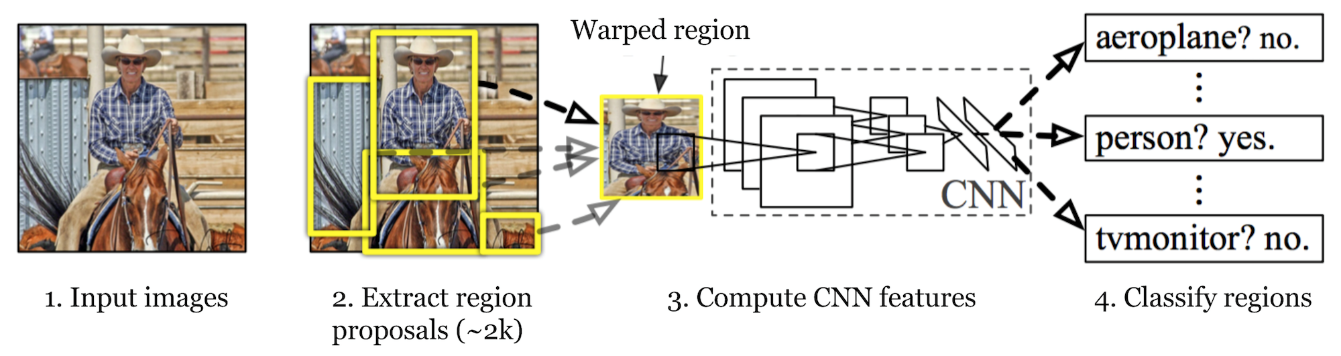
\includegraphics[width=1\linewidth]{Figs/rcnnSche.png}}
	\caption{Schematic of the R-CNN pipeline.}
	\label{fig:rcnnSche}
\end{figure}
\subsubsection{FastRCNN}
The main disadvantage of the R-CNN method is its slow speed. This is mainly because each regional proposal is passed through CNN separately, which is very time-consuming. In order to improve the speed, Girshick introduced a target detection method called Fast R-CNN in \cite{DBLP:journals/corr/Girshick15}. Fast R-CNN can improve the speed of object detection, mainly by passing the image forward through CNN only once, rather than once for each region performed by R-CNN. As in R-CNN, the region proposal method first divides the image into category-independent regions, creating a region of interest (RoI). Then, the entire image is processed by a CNN, which does a convolutional feature map of the image. Next, for each regional proposal, the RoI pool layer using spatial pyramid pool \cite{DBLP:journals/corr/HeZR014} is applied to the feature map. This will convert each RoI into a fixed-size vector. Then, the feature vectors are processed by fully connected layers, which are divided into two different output layers. One of the output layers is the softmax layer, which estimates probability estimates for object classes. The other layer is the bounding box regressor, which outputs a refined estimate of the bounding box for each object class. Figure \ref{fig:fastArc} shows how an image is processed by Fast R-CNN.
\begin{figure}
	\centerline{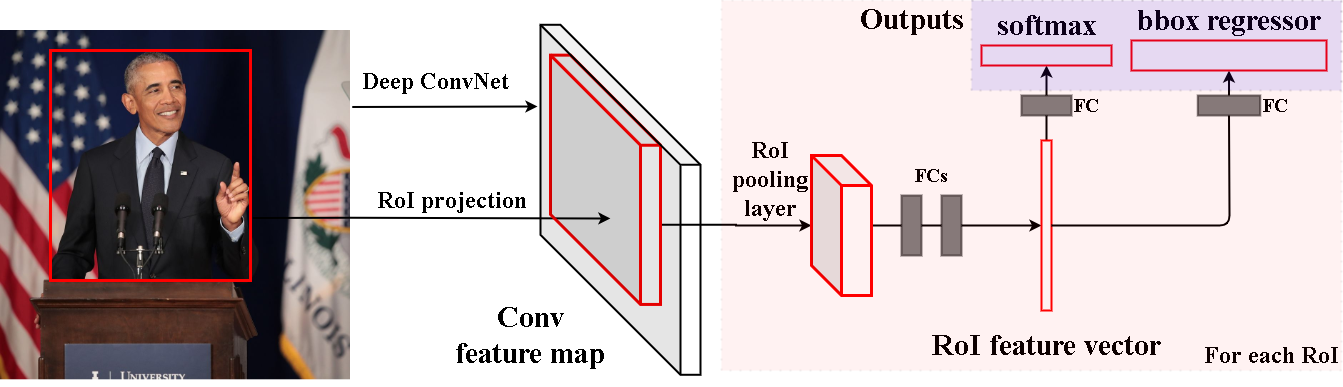
\includegraphics[width=0.5\linewidth]{Figs/fastArc.png}}
	\caption{The architecture of Fast RCNN.}
	\label{fig:fastArc}
\end{figure}
The model is optimized for a loss combining two tasks (classification + localization):
\begin{table}[]
	\caption{Some definitions for calculating FastRCNN losses.}
	\begin{tabular}{|l|l|}
		\hline
		Symbol                                          & Explanation                                                                                                                                                                                                  \\ \hline
		u                                              & \begin{tabular}[c]{@{}l@{}}True class label, \(u \in 0,1,…,K\); by convention, the catch-all background\\ class has \(u=0\)\end{tabular}                                                                    \\ \hline
		p                                              & \begin{tabular}[c]{@{}l@{}}Discrete probability distribution (per RoI) over K + 1 classes:\\ \(p=(p_0,…,p_K)\), computed by a softmax over the K + 1 outputs of a fully\\ connected layer.\end{tabular} \\ \hline
		v                                              & True bounding box \(v=(v_x, v_y, v_w, v_h)\).                                                                                     \\ \hline
		\begin{tabular}[c]{@{}l@{}} \(t^u\)\end{tabular} & Predicted bounding box correction, \(t^u=(t^u_x, t^u_y, t^u_w, t^u_h)\).                                                                                                                                                                         \\ \hline
	\end{tabular}
\end{table}
The loss function sums up the cost of classification and bounding box prediction: \(\mathcal{L} = \mathcal{L}_{cls} + \mathcal{L}_{box}\). For “background” RoI, \(\mathcal{L}_{box}\) is ignored by the indicator function
\(f [u \geq 1]\), defined as in equation \ref{eq:mathbb}.
\begin{equation}
	\label{eq:mathbb}
f [u >= 1] = \begin{cases}
	1  & \text{if } u \geq 1\\
	0  & \text{otherwise}
\end{cases}
\end{equation}
The overall loss function is:
\begin{equation}
	\mathcal{L}(p, u, t^u, v) = \mathcal{L}_{cls} (p, u) + f [u \geq 1] \mathcal{L}_{box}(t^u, v)
\end{equation}\begin{equation}
	\mathcal{L}_{cls}(p, u) = -\log p_u
\end{equation}
\begin{equation}
	\mathcal{L}_{box}(t^u, v) = \sum_{i \in \{x, y, w, h\}} L_1^{smooth} (t^u_i - v_i)
\end{equation}
The bounding box loss \(\mathcal{L}_{box}\) should measure the difference between \(t^u_i\) and \(v_i\) using a robust loss function. The smooth L1 loss is adopted here and it is claimed to be less sensitive to outliers.
\subsubsection{FasterRCNN}
Fast R-CNN passing the speed of object detection by passing the image forward through the CNN only once, instead of forward passing through each region of interest in the image. For Fast R-CNN, the bottleneck lies in the image segmentation method usually implemented on the CPU. In order to solve this problem, Ren et al. A method called Faster R-CNN is proposed in \cite{DBLP:journals/corr/RenHG015}. Faster R-CNN eliminates the need for CPU computing by introducing the idea of a Region Proposal Networks (RPNs). The region proposal network to region proposed by sliding a small network on the convolutional feature map. At each location, the small network takes a window of the convolution feature map and converts it into a feature vector. This feature vector is then input into two different fully connected layers, one layer performs bounding box regression, and the other layer is a classification layer that predicts objective scores. The objectivity score is a prediction of the probability that the predicted bounding box contains only one object compared to the background.
\\For each position, RPN makes several predictions relative to a fixed number of reference frames, which are called anchors. You can anchor as a suggested border for each sliding window position. In \cite{DBLP:journals/corr/RenHG015}, anchors are created in 3 ratios and 3 different aspect ratios, and each position provides a total of 9 different anchors. This means that RPN has 9 bounding boxes at each sliding window position, and each anchor point has one bounding box.
\begin{figure}
	\centerline{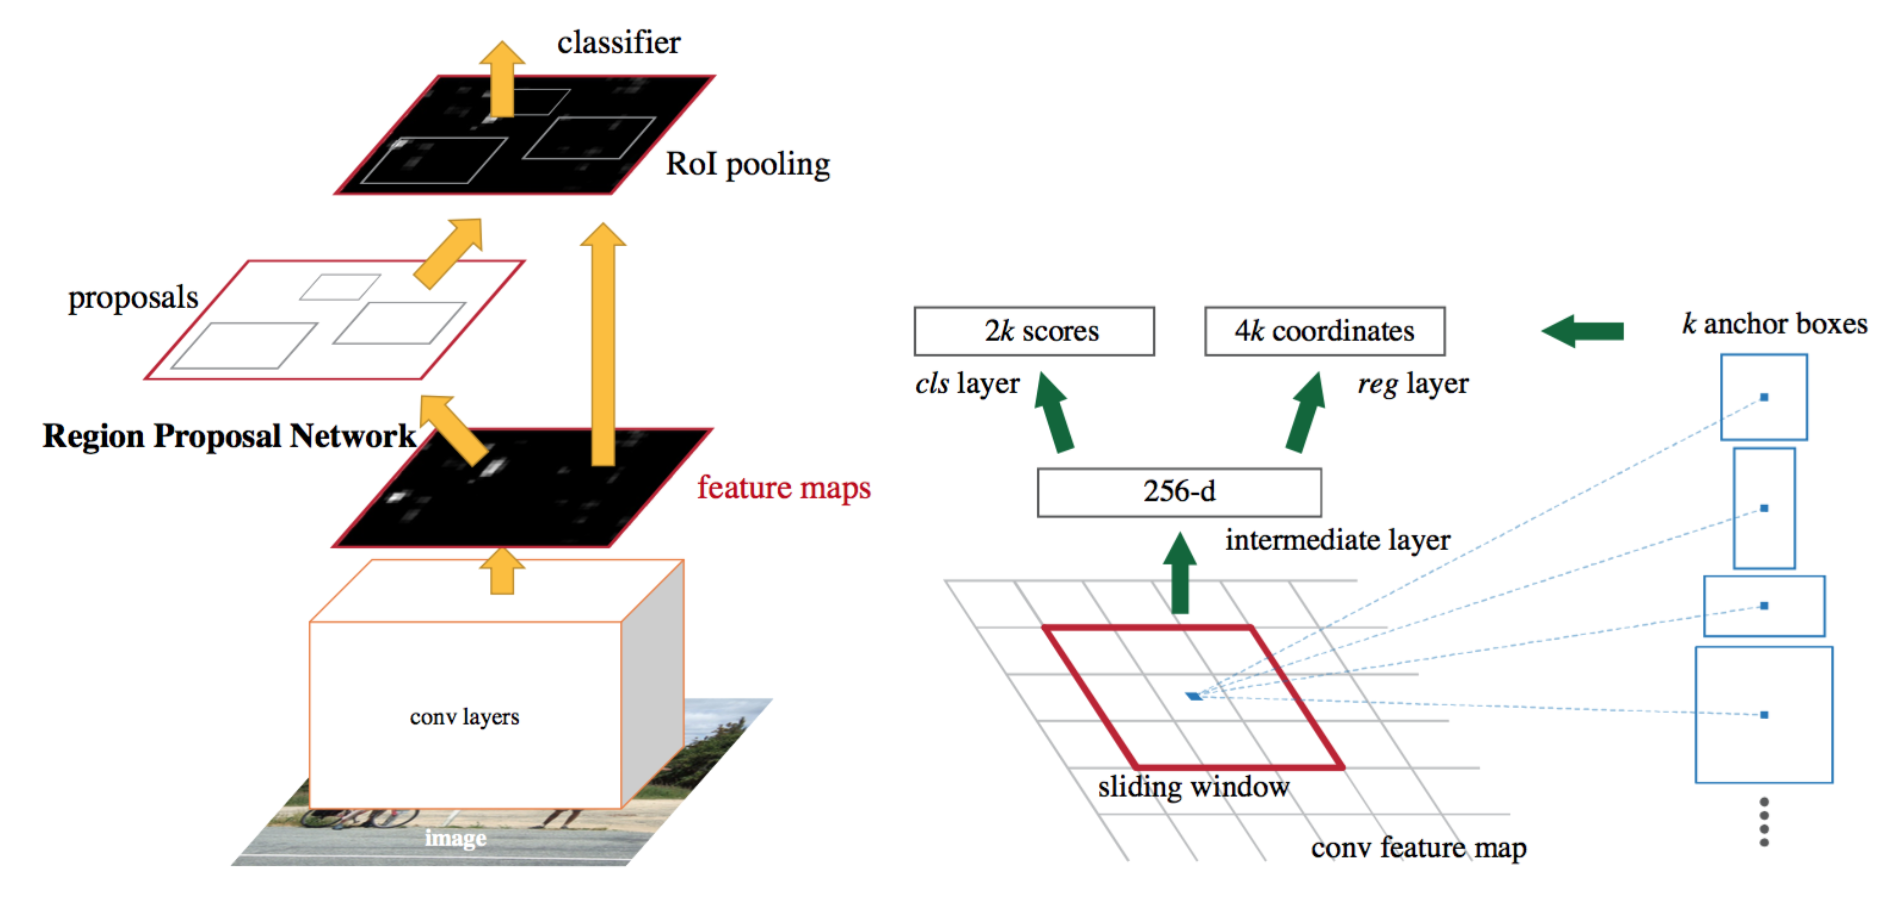
\includegraphics[width=0.5\linewidth]{Figs/faster.png}}
	\caption{An illustration of Faster RCNN model.}
	\label{fig:faster}
\end{figure}
\\The regions generated by RPN are then used as region suggestions in fast RCNN. By using RPN, Faster R-CNN eliminates the time-consuming image segmentation required in Fast R-CNN. By using a single CNN for RPN and fast R-CNN, the speed is further increased. This also means that the Faster R-CNN can be trained end-to-end by first training the RPN to propose a region, and then using the region proposal to train the Fast R-CNN.
\\Faster R-CNN is optimized for a multi-task loss function, similar to fast R-CNN.
\begin{table}[]
	\label{tab:noteFaster}
	\caption{Some definitions for calculating FasterRCNN losses.}
	\begin{tabular}{|l|l|}
		\hline
		Symbol & Explanation                                                                                                                                                           \\ \hline
		\(p_i\)      & Predicted probability of anchor i being an object.                                                                                                                    \\ \hline
		\(p_i^*\)      & Ground truth label (binary) of whether anchor i is an object.                                                                                                         \\ \hline
		\(t_i\)      & Predicted four parameterized coordinates.                                                                                                                             \\ \hline
		\(t_i^*\)      & Ground truth coordinates.                                                                                                                                             \\ \hline
		\(N_{cls}\)      & Normalization term, set to be mini-batch size ($\sim$256) in the paper.                                                                                               \\ \hline
		\(N_{box}\)      & \begin{tabular}[c]{@{}l@{}}Normalization term, set to the number of anchor locations ($\sim$2400) in\\ the paper.\end{tabular}                                        \\ \hline
		$\lambda$      & \begin{tabular}[c]{@{}l@{}}A balancing parameter, set to be $\sim$10 in the paper (so that both \(\mathcal{L}_{cls}\) and\\ \(\mathcal{L}_{box}\) terms are roughly equally weighted).\end{tabular} \\ \hline		
	\end{tabular}
\end{table}
With notation in Table \ref{tab:noteFaster} the multi-task loss function combines the losses of classification and bounding box regression:
\begin{equation}
	\mathcal{L}_{reg} = \mathcal{L}_{cls} + \mathcal{L}_{box}
\end{equation}
\begin{equation}
	\mathcal{L}(\{p_i\}, \{t_i\})= \frac{1}{N_{cls}} \sum_i \mathcal{L}_{cls} (p_i, p^*_i) + \frac{\lambda}{N_{box}} \sum_i p^*_i \cdot L_1^{smooth}(t_i - t^*_i) \\
\end{equation}
where \(\mathcal{L}_{cls}\) is the log loss function over two classes, as we can easily translate a multi-class classification into a binary classification by predicting a sample being a target object versus not. \(L_1^{smooth}\) is the smooth L1 loss.
\begin{equation}
	\mathcal{L}_{cls} (p_i, p^*_i) = - p^*_i \log p_i - (1 - p^*_i) \log (1 - p_i)
\end{equation}
\subsubsection{MaskRCNN}
The mask R-CNN is an extension of Faster R-CNN proposed by He et al in \cite{DBLP:journals/corr/HeGDG17}. In addition to object detection, Mask R-CNN can also perform object instance segmentation. Segmentation is achieved by adding a third branch to Faster R-CNN, which outputs an object mask for each detected object. In order to improve the segmentation, a method called RoIAlign is introduced to extract more accurate feature maps for each RoI. RoIAlign uses bilinear interpolation instead of quantizing the feature map to calculate the exact value of the feature map.
\begin{figure}
	\centerline{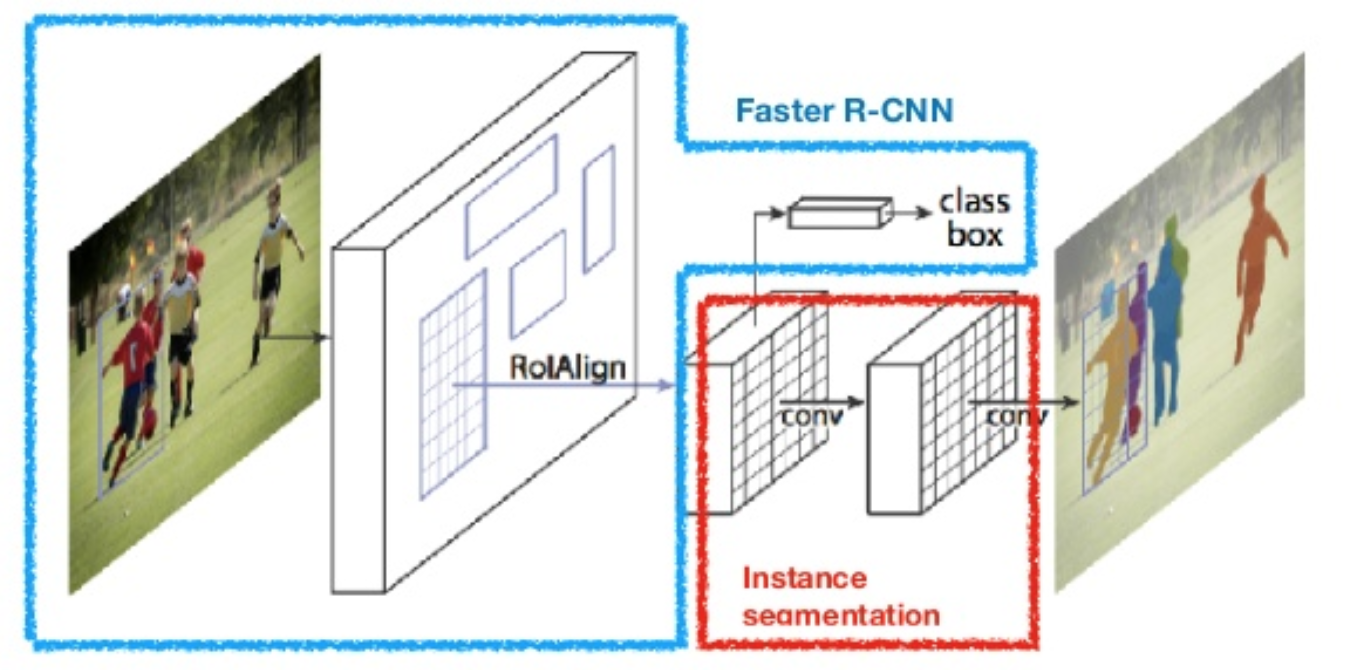
\includegraphics[width=0.5\linewidth]{Figs/maskrcnn.png}}
	\caption{The Mask RCNN framework for instance segmentation.}
	\label{fig:maskrcnn}
\end{figure}
The author of \cite{DBLP:journals/corr/HeGDG17} found that Mask R-CNN has a higher average accuracy than Faster R-CNN in target detection. It turns out that this is partly due to the use of RoIAlign and partly due to the multi-task loss used to train Mask R-CNN. Mask R-CNN has a multi-task loss function, which can simultaneously consider classification, bounding box regression and object segmentation.
The multi-task loss function of Mask R-CNN combines the loss of classification, localization and segmentation mask: 
\begin{equation}
	\mathcal{L} = \mathcal{L}_{cls} + \mathcal{L}_{box}+ \mathcal{L}_{mask}
\end{equation}
where \(\mathcal{L}_{cls}\) and \(\mathcal{L}_{box}\) are same as in Faster R-CNN.
The mask branch generates a mask of dimension m x m for each RoI and each class; K classes in total. Thus, the total output is of size \(K \cdot m^2\). Because the model is trying to learn a mask for each class, there is no competition among classes for generating masks. \(\mathcal{L}_{mask}\) is defined as the average binary cross-entropy loss, only including k-th mask if the region is associated with the ground truth class k.
\begin{equation}
	\mathcal{L}_{mask} = - \frac{1}{m^2} \sum_{1 \leq i, j \leq m} \big[ y_{ij} \log \hat{y}^k_{ij} + (1-y_{ij}) \log (1- \hat{y}^k_{ij}) \big]\
\end{equation}
where \(y_{ij}\) is the label of a cell (i, j) in the true mask for the region of size m x m; \(\hat{y}_{ij}^k\) is the predicted value of the same cell in the mask learned for ground-truth class k.
\subsection{YOLO model family}
\subsubsection{YOLO}
In \cite{DBLP:journals/corr/RedmonDGF15}, a novel object detection method is introduced, called YOLO, which means "You Only Look Once". Unlike R-CNN and its successors, YOLO does not use any region proposal method, but uses a single CNN to predict bounding boxes and classes. 
\\In YOLO, the input image is first divided into S × S grids. Then, each grid unit is responsible for predicting the bounding box B and the confidence score of each bounding box. The formula for calculating the confidence score is \(Pr(Object)*IoU_{pred}^{gt}\), where Pr(Object) is the predicted probability that the box contains an object, and \(IoU_{pred}^{gt}\) is the estimated intersection over union (IoU) between the predicted box and the ground truth box. For each grid unit, the probability of object categories C can also be predicted, and these probabilities are conditioned on the unit containing the object. The predicted box and class probabilities are then combined into a single score for each class and box. 
\\Equation \ref{eq:yolo} comes from the introduction by YOLO in \cite{DBLP:journals/corr/RedmonDGF15}, which shows how class prediction and box prediction are combined. As shown in the original paper, \(Pr(Class_i)\) is used as a simplified representation of \(Pr(Class_i|Object)\).
\begin{equation}
	\label{eq:yolo}
	Pr(Class_i|Object)*Pr(Object)*IoU^{gt}_{pred} = Pr(Class_i)*IoU^{gt}_{pred}
\end{equation}
This score not only explains the probability that the box contains class \(i\), \(Pr(Class_i)\), but also how to estimate the predicted box to fit the ground truth box \(Pr(Object)*IoU_{pred}^{gt}\). 
%Figure \ref{fig:yoloworkflow} shows how to split the image into a grid, and how the cell with the dot as the center predicts different bounding boxes. The predicted bounding box is then combined with the class probabilities also obtained from the image grid to produce the final object detection.
%\begin{figure}
%	\centerline{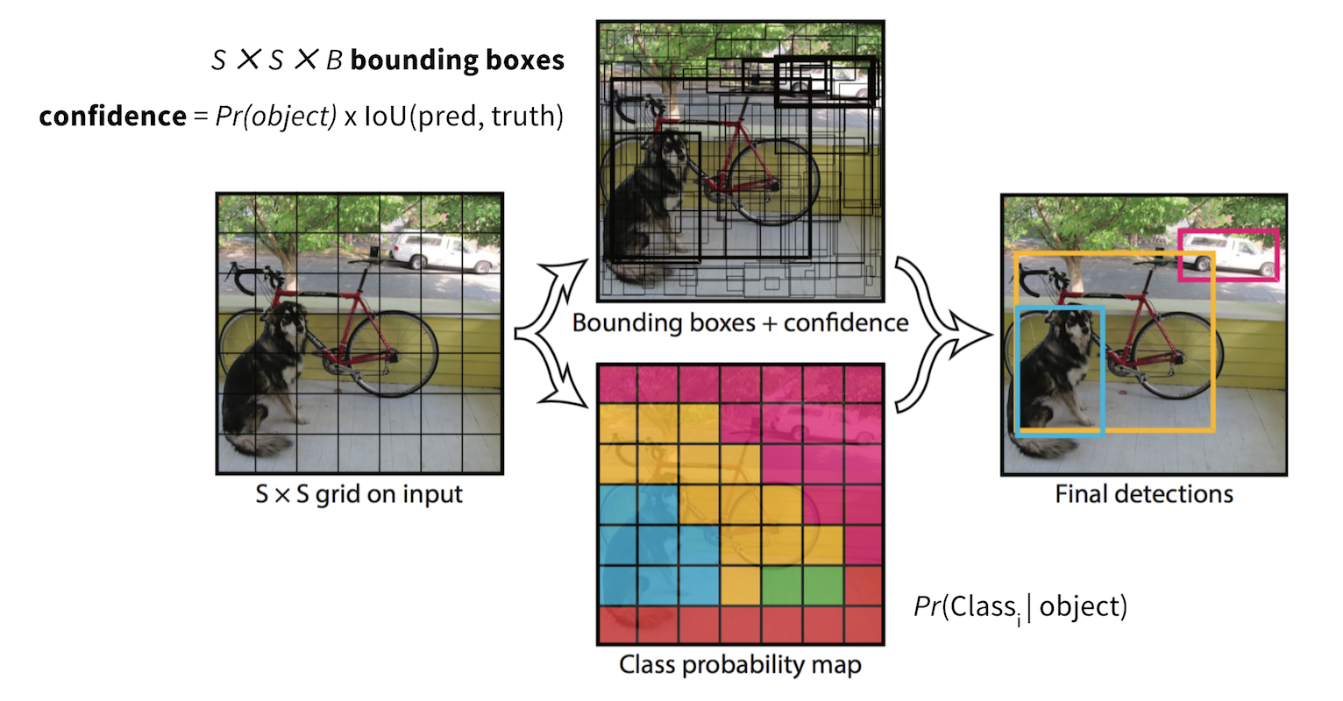
\includegraphics[width=1\linewidth]{Figs/yoloworkflow.png}}
%	\caption{The workflow of YOLO model.}
%	\label{fig:yoloworkflow}
%\end{figure}
The base model \ref{fig:yolo-network} is similar to GoogLeNet with inception module replaced by 1x1 and 3x3 conv layers. The final prediction of shape S×S×(5B+K) is produced by two fully connected layers over the whole conv feature map.
\begin{figure}
	\centerline{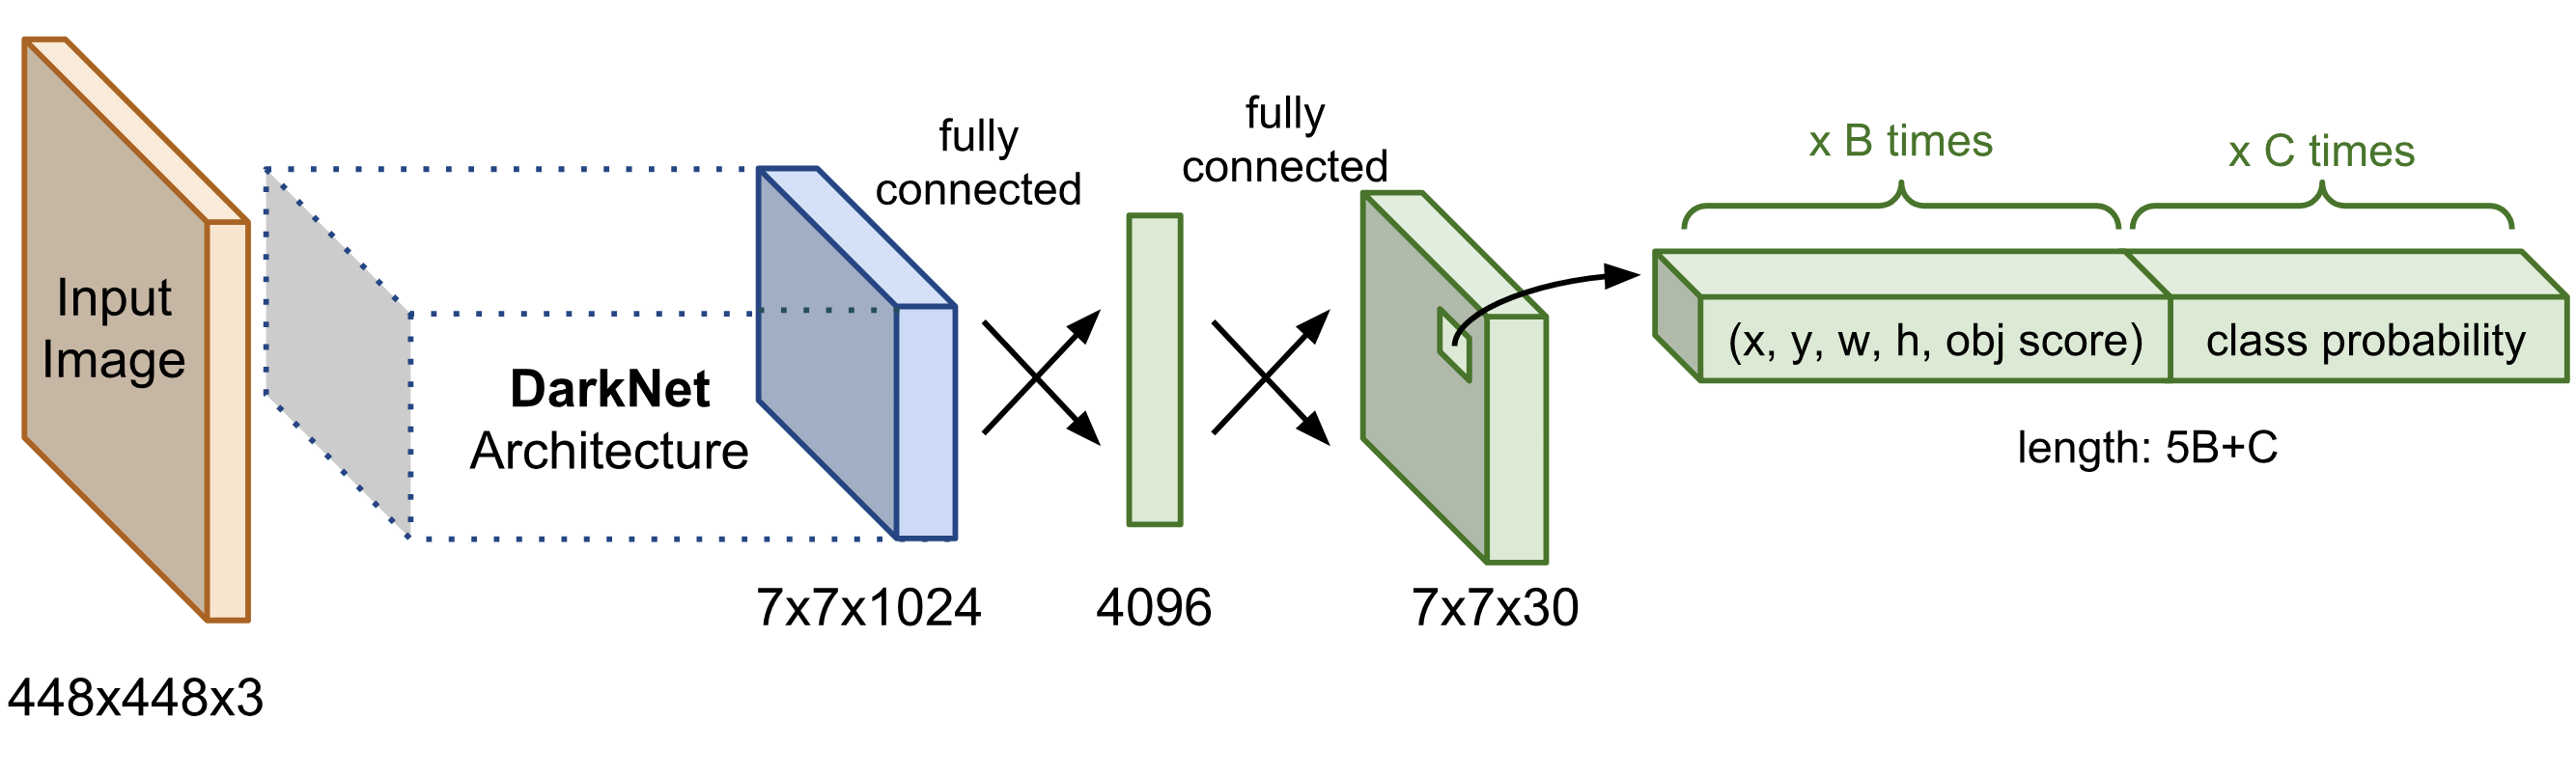
\includegraphics[width=1\linewidth]{Figs/yolo-network.png}}
	\caption{The network architecture of YOLO.}
	\label{fig:yolo-network}
\end{figure}
\subsubsection{YOLOv2}
In order to improve YOLO, Redmon et al. proposed a method called YOLOv2 in \cite{DBLP:journals/corr/RedmonF16}. YOLOv2 is a modified version of YOLO, designed to improve speed and accuracy.
Similar to Faster R-CNN, YOLOv2 uses anchor points when predicting the bounding box. For each grid unit, YOLOv2 generates a bounding box by predicting the offset of 5 anchor points. It is now also possible to predict the class for each anchor point instead of each grid unit, and also provide an objective score for each anchor point. As in YOLO, the class is predicted under the condition that the object \(Pr(Class_i|Object)\) exists. Objectivity is calculated as the estimated IoU between the predicted box and the estimated ground truth box \(IoU_{pred}^{gt}\). YOLOv2 also uses a new method to determine the anchor point size. YOLOv2 is different from manually selecting anchor points in Faster R-CNN, but uses k-means clustering on the training data to generate anchor points that are more suitable for the data.
In order to increase speed, a CNN architecture called Darknet-19 is introduced in YOLOv2. Darknet-19 is able to achieve higher image classification accuracy than both the widely used VGG-16 [33] and the custom network previously used in YOLO [40]. It manages to do this while only using 5.58 * 109 floating point operations per forward pass, compared to 30.69 * 109 operations in VGG-16 and 8.52 * 109 operations in the network previously used in YOLO.
\subsubsection{YOLOv3}
YOLOv3 includes a further improvement of YOLOv2 proposed by Redmon et al in \cite{DBLP:journals/corr/abs-1804-02767}. Similar to the feature pyramid network (FPN) described in \cite{DBLP:journals/corr/LinDGHHB16}, in YOLOv3, the box will be predicted at 3 different scales. This YOLOv3's ability to detect small objects, which was struggling with earlier versions of YOLO.
Inspired by the residual network proposed in \cite{DBLP:journals/corr/HeZRS15}, Darknet-19 was extended to include a residual layer. This new CNN architecture is called Darknet-53 because it has a total of 53 convolutional layers. Compared with Darknet-19, Darknet-53 has higher accuracy but slower speed.
%\vspace{-1.6cm}
\subsubsection{YOLOv4}
So far, YOLOv4 is the latest and most advanced iteration \cite{bochkovskiy2020yolov4}. It has the fastest running speed and can be used for optimization of production systems and parallel computing. Some of the new technologies adopted in YOLOv4 are: (1) weighted residual connection, (2) cross-stage-partial connection, (3) cross mini-batch processing, (4) normalization (CmBN), (5) self-confrontation training, (6) Mish-activation, etc. In order to obtain higher precision values, YOLOv4 uses Dense Block, which is a deeper and more complex network. Similarly, the backbone of its function extractor uses CSPDarknet-53, which deploys CSSP connection with Darkenet-53 of the early YOLOv3. In addition to CSPDarknet-53, YOLOv4's architecture also includes SPP add-on modules, PANet path aggregation neck and YOLOv3 anchor-based head. SPP blocks are stacked on CSPDarknet53 to increase the receiving field that can discretize the most significant context features and ensure that its network operation speed will not decrease. Similarly, PANet is used to aggregate parameters from multiple backbone levels, instead of the FPN used in YOLOv3.
\section{Object tracking algorithms}
\subsection{SORT}
SORT is a tracking algorithm introduced by Bewley et al in \cite{DBLP:journals/corr/BewleyGORU16}. SORT is designed to perform multi-object tracking in a tracking-by-detection system. In order to achieve real-time processing, SORT is deliberately kept simple to avoid performing complex and time-consuming tasks. In order to make up for its lack of complexity, SORT uses CNN-based object detectors instead of relying on more accurate object detection. 
For each new frame, SORT first propagates objects that are already tracked into the current frame. The new positions of these already tracked objects are predicted using a Kalman filter \cite{10.1115/1.3662552} with a linear constant velocity model. Next, an object detection algorithm detects objects present in the current frame. These detected objects are then compared to already tracked objects and a cost-matrix is created. This cost-matrix is calculated as the IoU between each detection and each of the already tracked objects. Detections are then assigned to already tracked objects using the Hungarian method \cite{doi:10.1002/nav.3800020109}. When an object is detected in several consecutive frames and does not overlap with any tracked object, a new trajectory is created. To further explain this point, the object model is represented by equation \ref{eq:kal}, where u, v, s, and r represent the horizontal pixel position, vertical pixel position, area, and aspect ratio of the target object, respectively.
\begin{equation}
	\label{eq:kal}
	X=[u, v, s, r, \dot{u}, \dot{v}, \dot{s}]
\end{equation}
As long as the detection is linked to the target object, the detected bounding box is used to inform the target state, and the Kalman filter is used to solve the level and velocity values. This helps to identify the target's identity in consecutive frames and helps tracking.
\subsection{DeepSORT}
DeepSORT is built to reduce the number of identity switches and integrate appearance information into the tracking process proposed in SORT. Similar to SORT, DeepSORT uses Kalman filter to process state estimation. The difference between DeepSORT and SORT is that it utilizes other technologies when assigning detection to the tracked object.
The first improvement of DeepSORT is the deep appearance descriptor.  To obtain the appearance information of detections and tracks, an appearance descriptor is used to extract features from detection images and track images from previous frames. The appearance descriptor is a CNN trained on large-scale person re-identification dataset. It is able to extract features in a way that features from the same identity are close together and features from different identities are far away from each other in the feature space. The overview of the network architecture of the re-identification model used in DeepSORT framework is shown Table \ref{tab:desarchitecture}.
This thesis customizes the CNN on a custom egocentric hand re-identification dataset, Micand32S. Detail training process is explained in chapter 3, sub-section 3.2.2. Appearance descriptors are computed by forwarding each bounding box through a CNN that has been pretrained on a person re-identification dataset. The appearance descriptor of each new detection is then compared to the appearance descriptors of already tracked objects by calculating the cosine distance between descriptors. Tracked objects and their appearance descriptors are also saved for 30 frames after they are lost so that Deep SORT has the ability to resume tracking identities that have been lost for a number of frames. Using appearance descriptors in this way gives DeepSORT the ability to find a previously tracked object even if it has been occluded for a number of frames.
\begin{table}[]
	\centering
	\label{tab:desarchitecture}
	\caption{Overview of the CNN architecture \cite{DBLP:journals/corr/WojkeBP17}. The final batch and L2 normalization projects onto the unit hyper-sphere.}
	\begin{tabular}{|l|l|l|}
		\hline
		Name                       & Patch Size/Stride & Output Size \\ \hline
		Conv1                      & 3x3/1             & 32x128x64   \\ \hline
		Conv2                      & 3x3x1             & 32x128x64   \\ \hline
		Max Pool 3                 & 3x3/2             & 32x64x32    \\ \hline
		Residual 4                 & 3x3/1             & 32x64x32    \\ \hline
		Residual 5                 & 3x3/1             & 32x64x32    \\ \hline
		Residual 6                 & 3x3/2             & 64x32x16    \\ \hline
		Residual 8                 & 3x3/2             & 128x16x8    \\ \hline
		Residual 9                 & 3x3/1             & 128x16x8    \\ \hline
		Dense 10                   &                   & 128         \\ \hline
		Batch and \(L_2\) normalization &                   & 128         \\ \hline
	\end{tabular}
	\vspace{-1cm}
\end{table}
The second improvement of DeepSORT is the data association. With the estimated position of the existing tracks and the appearance descriptor, we can now associate new detection results to the existing tracks in each coming frame. A detection confidence threshold td is used to filter out all the detections with confidence lower than the threshold. New detections have to pass this threshold to be candidates of data association. The Deep SORT algorithm uses a cost matrix to represent the spatial and appearance similarities between each new detections and existing tracks. It is integrated by two distance values. The first distance is shown in equation \ref{eq:mahalanobis} representing the spatial information:
\begin{equation}
	\label{eq:mahalanobis}
	d^{(1)}(i,j)=(d_j-y_i)^TS^-1_i(d_j-y_i)
\end{equation}
where \((y_i, S_i)\) are the projection of the i-th track in measurement space and \(d_j\) is the j-th new detection. This is the Mahalanobis distance \cite{hastie2009elements} between j-th new detection and estimated position of i-th. The Mahalanobis distance measures how the position of a new detection differs from the positions of already tracked objects in terms of standard deviations from the mean of the tracked objects. This metric allows DeepSORT to avoid assigning a new detection to an already existing track where the frame-to-frame motion would be unreasonable. The second distance is show in equation \ref{eq:appearance} representing the appearance information.
\begin{equation}
	\label{eq:appearance}
	d^{(2)}(i,j)=min(1-r_j^Tr_k^{(i)}|r_k^{(i)}\in R_i))
\end{equation}
where r is the appearance descriptor and Ri are the appearances of the last 100 object associated with the i-th track. Each distance is accompanied with a gate function \(b_{i,j}^1\)and \(b_{i,j}^2\) which are equal to 1 if the distance is smaller than pre-defined threshold and 0 otherwise. The integrated cost matrix is show in equation \ref{eq:integrated}:
\begin{equation}
	\label{eq:integrated}
	c_{i,j} = \lambda d^{(1)}(i,j) + (1-\lambda)d^{(2)}(i,j)
\end{equation}
With a gate matrix \(b_{i,j}\) which equals to 1 only when both spatial and appearance gate function are equal to 1 and otherwise 0, indicating whether (i, j) is a valid match for both spatial and appearance. In each new frame, the new detections are associated with existing tracks using this cost matrix and gate matrix.
Track handling is processed as follow: every time a new detection is successfully associated with an existing track, the detection is added to the track and the unassociated age of the track is zero. When new detections fail to associate with existing tracks in frame f, the new detections are initialized as Tentative tracks. The original Deep SORT algorithm checks that the Tentative tracks are associated with new detections in each of the  \((f+1), (f+2), ... (f+t_{tentative})\) frames. If successfully associated, the track is updated as Confirmed track. Otherwise, the Tentative track is deleted immediately. As for the existing tracks that fail to associate with new detections in each frame, their unassociated ages will increase by one. If the unassociated age exceeds the max age threshold, the track will also be deleted.
\section{Egocentric vision datasets}\label{sec:datasets}
\subsection{GTEA family datatsets}
Georgia Tech Egocentric Activity Datasets (GTEA) \cite{5995444} contains 7 types of daily activities, each performed by 4 different subjects. The camera is mounted on a cap worn by the subject. 
GTEA Gaze \cite{fathigaze} dataset is collected using Tobii eye-tracking glasses. It consists of 17 sequences, performed by 14 different subjects. GTEA Gaze+ \cite{7298625} is collected by using SMI eye-tracking glasses at Georgia Tech's AwareHome. This dataset consists of 7 meal-preparation activities, performed by 26 subjects. Subjects perform the activities based on the given recipes. Activities are: American Breakfast, Pizza, Snack, Greek Salad, Pasta Salad, Turkey Sandwich and Cheese Burger. SMI glasses record a HD video of subject’s activities at 24 frames per second. They also record subject's gaze at 30 fps. For each activity, ELAN is used to annotate its actions. An activity is a meal-preparation task such as making pizza, and an action is a short temporal segment such as putting sauce on the pizza crust, dicing the green peppers, washing the mushrooms. The authors have completed more than half of the annotations. The current version contains 37 videos with gaze tracking and action annotations. Audio files are also available on request.
%\begin{figure}
%	\centerline{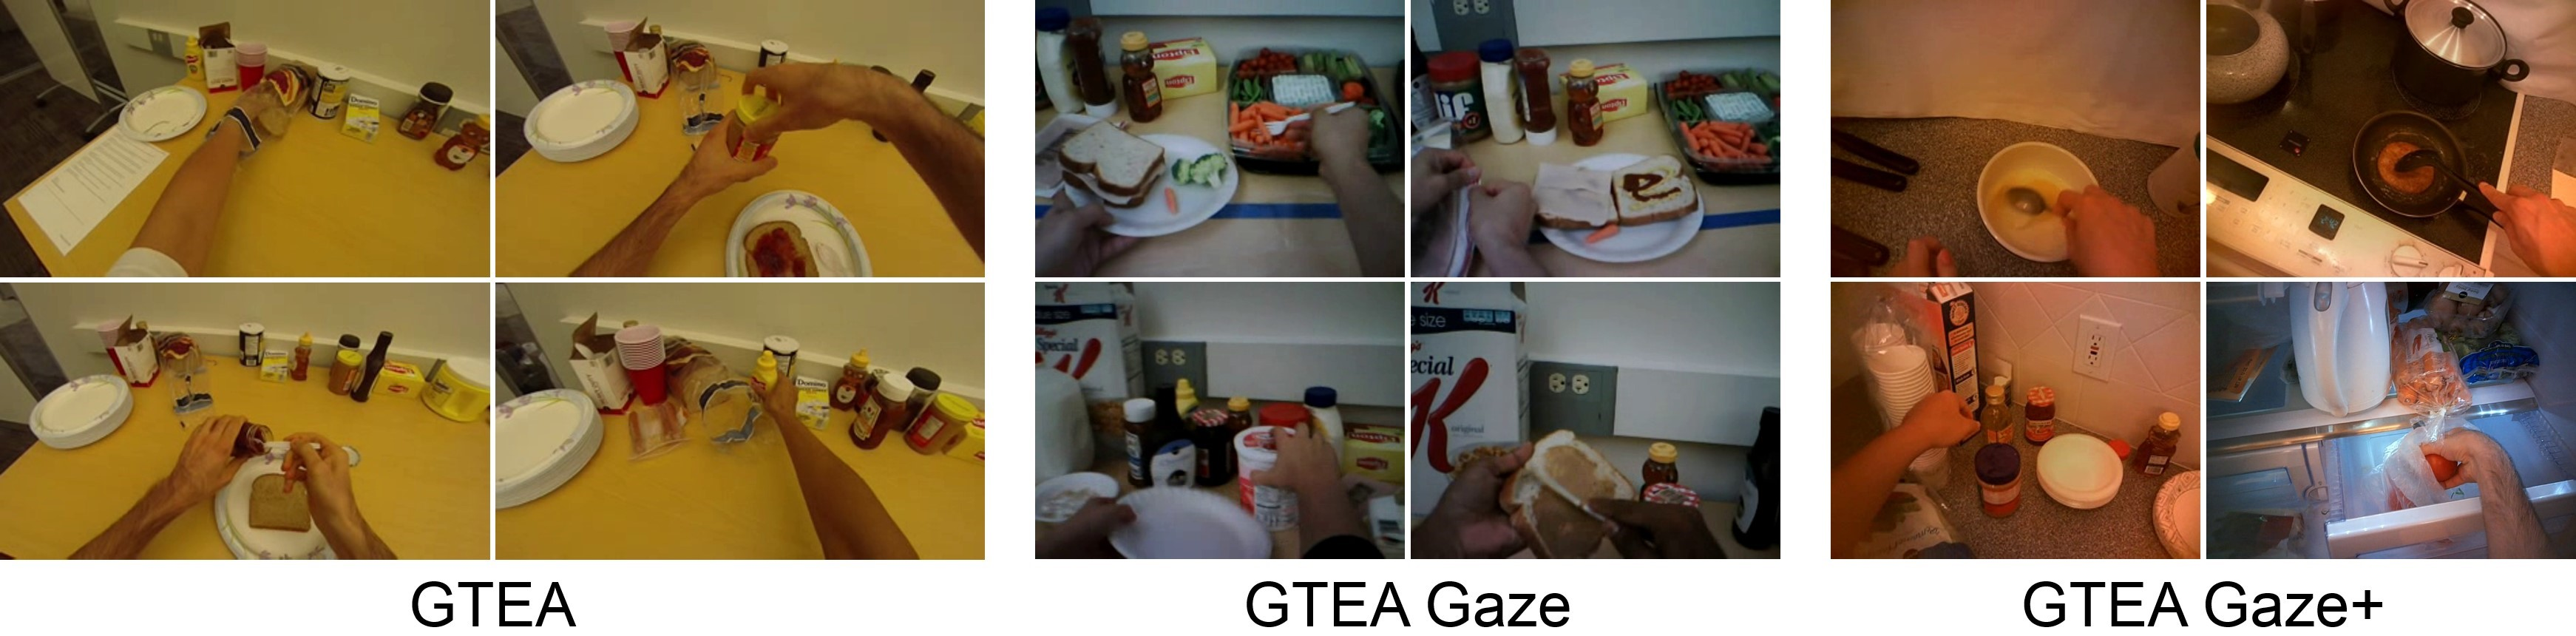
\includegraphics[width=1\linewidth]{Figs/GTEA.jpg}}
%	\caption{Upshots from GTEA family datasets.}
%	\label{fig:gtea}
%\end{figure}
EGTEA Gaze+ \cite{li2020eye} is the largest and most comprehensive dataset for FPV actions and gaze up to date. This dataset coms with HD videos (1920x960), audios, gaze tracking data, frame-level action annotations and pixel-level hand masks at sampled frames. EGTEA Gaze+ is a major expansion of GTEA Gaze+. Specifically, this new datasets EGTEA Gaze + contains 29 hours (withdrawn status) cooking events from 86 independent sessions on 32 topics of 32 subjects performing 7 different meal preparation tasks. These videos have audio and gaze tracking (30Hz). The authors also provide human annotations for actions (human-object interactions) and hand masks. Action annotations include 10325 fine-grained action examples, such as "cut green peppers" or "pour condiments in a condiment container into a salad". These pixel-level hand annotations include 15,176 hand masks in 13,847 frames from the video of 200 action categories sparsely sampled from all 86 sessions of the datasets. Post-processing EGTEA Gaze+ dataset for the thesis’s framework is conducted as follow: The original data in the EGTEA Gaze + dataset is processed into COCO standard in order to be used in the framework. The mask image is converted into binary mask image by thresholding and then applying a contour calculation algorithm of the hand area. At last, the binary mask is converted to the RLE (run length encoding) standard which is usable data in the framework. In the scope of this thesis, the 4 datasets GTEA, GTEA Gaze, GTEA Gaze + and EGTEA Gaze + is regulated into GTEA family datasets.
\vspace*{-\baselineskip}
\begin{figure}
	\centerline{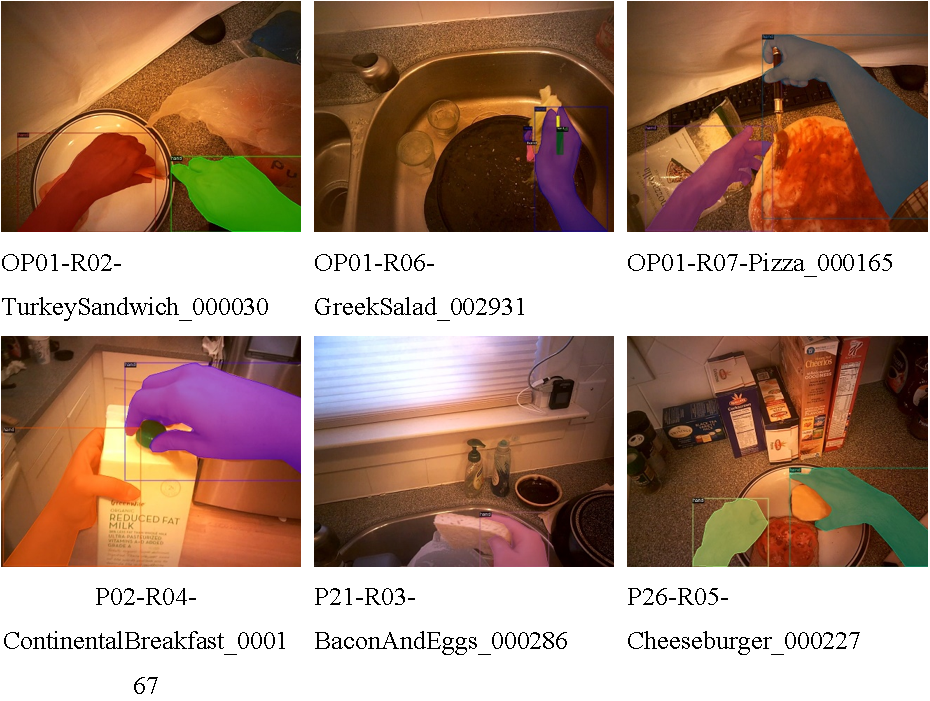
\includegraphics[width=1\linewidth]{Figs/postGTEA.png}}
	\caption{Hand masks after post-processing EGTEA Gaze+.}
	\label{fig:postgtea}
\end{figure}
\subsection{EgoHands dataset}
The EgoHand dataset, which is presented in \cite{10.1109/ICCV.2015.226} is a large dataset for hands in complex egocentric interactions. In order to create as realistic data sets as possible while still being able to carry out some experimental control, the author collected data from different pairs of four pairs of participants, who faced each other when faced with different activities. The authors chose four activities that encourage interaction and gesture movement: (1) playing cards; (2) playing chess, in order to improve efficiency, they encourage participants to focus on speed rather than strategy; (3) solve 24 or 48 pieces of jigsaw puzzles; (4) play Jenga, which involves removing pieces from the 3d puzzle until it collapses. The context is also varied by collecting videos in 3 different locations: a table in a meeting room, a patio table in an outdoor courtyard, and a coffee table at home. The dataset is recorded for several days, and there was no restriction on the clothes of the participants, so there were many types, for example, short-sleeved and long-sleeved shirts, etc. Data is systematically collected from four actors who performed all four activities in all three locations, while randomly assigning participants to interact with each other, resulting in 4 × 4 × 3 = 48 unique video combinations. Each participant wore Google glasses, which recorded a 720 × 1280 video at a frequency of 30 Hz. In post-processing, the videos are synchronized in pairs with each other and each video pair is cut into exactly 90 seconds (2,700 frames). Ground truth is manually annotated from a random subset of 100 frames in each video (approximately one frame per second) using pixel-level manual masks. Each hand pixel has one of the following four tags: the left or right hand of the camera wearer ("my left hand" or "my right hand"), or the left or right hand of the social partner ("your left hand" or "your right hand "). The ground truth was created by six students who were told to mark any hand-shaped pixels they could see, including small hand areas caused by objects being occluded or truncated at frame boundaries. Importantly, compared with EGTEA Gaze+, this dataset defines "hand" as stopping on the wrist, and this job also includes the arm extending toward the participant's sleeve. In total, this dataset contains approximately 130,000 frames of video, of which 4,800 frames have a pixel-level ground truth consisting of 15,053 hands. The partner's hands appear in the vast majority of frames (left and right 95.2\% and 94.0\%, respectively), while the wearer's hand appears less (left and right 53.3\% and 71.1\%, respectively). This may be because one's own hand appears more often outside the camera's field of view, but the right hand appears more frequently because people tend to align their attention with the dominant hand (and all participants are right-handed). Figure \ref{fig:egohands} shows a sample frame with basic facts. This dataset is released on the public web with ground truth accessible through a Matlab API we provided by the authors.
\begin{figure}[!htb]
	\centerline{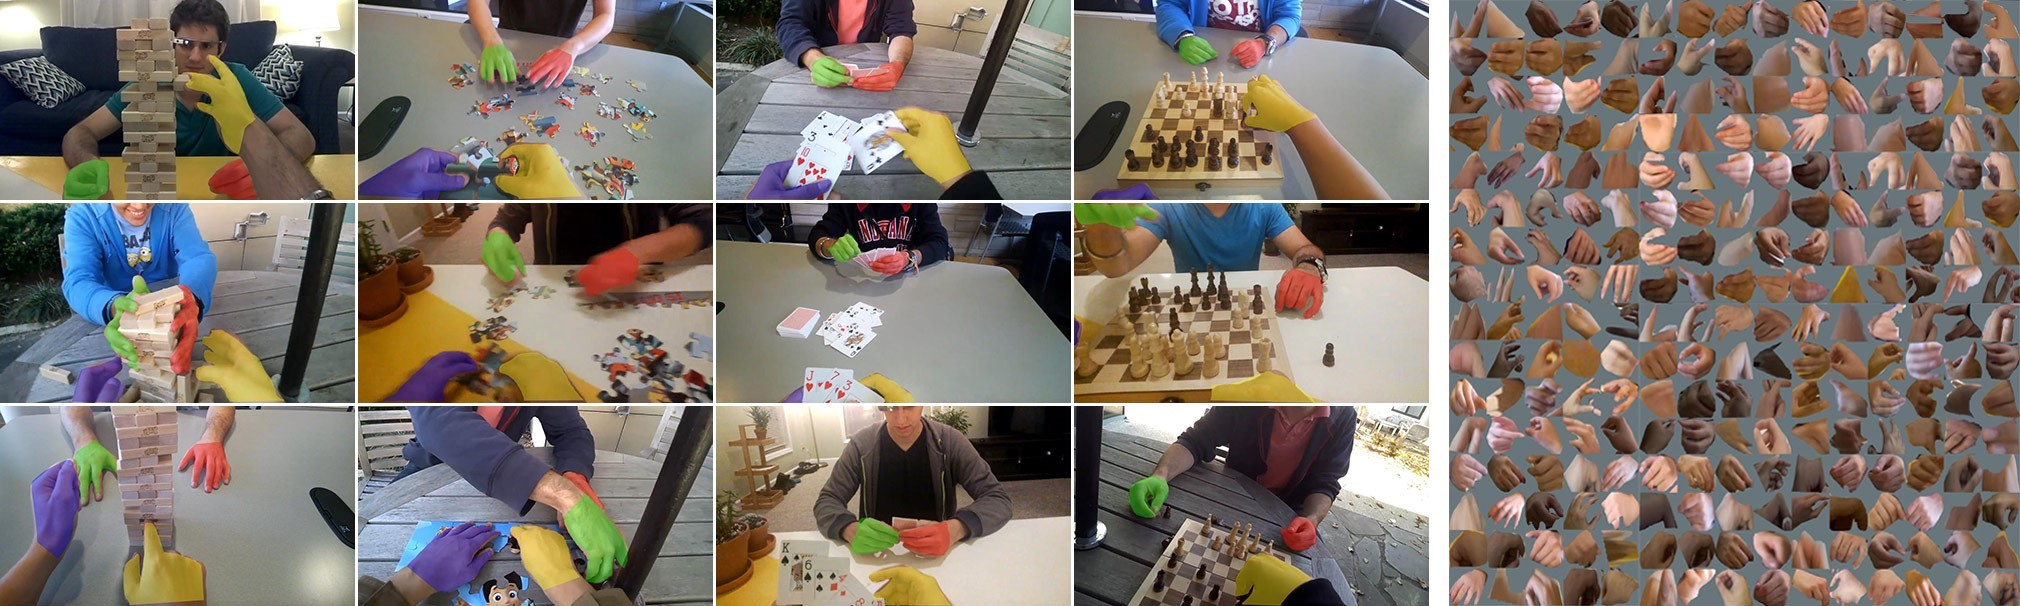
\includegraphics[width=1\linewidth]{Figs/egohands.jpg}}
	\caption{Visualizations of EgoHand dataset in \cite{10.1109/ICCV.2015.226}.}
	\label{fig:egohands}
\end{figure}
Post-processing EgoHands for the thesis’s framework is conducted as follow: The original annotations in EgoHands datasets consists of 4 categories: my left, my right, your left, your right. In the scope of this thesis, I just focus the hands appearing in egocentric video, therefore I convert all 4 categories into 1 category, “hand”. From the “.mat” format data, I dumped into “.json” format and feed to the framework.
%\begin{figure}
%	\centerline{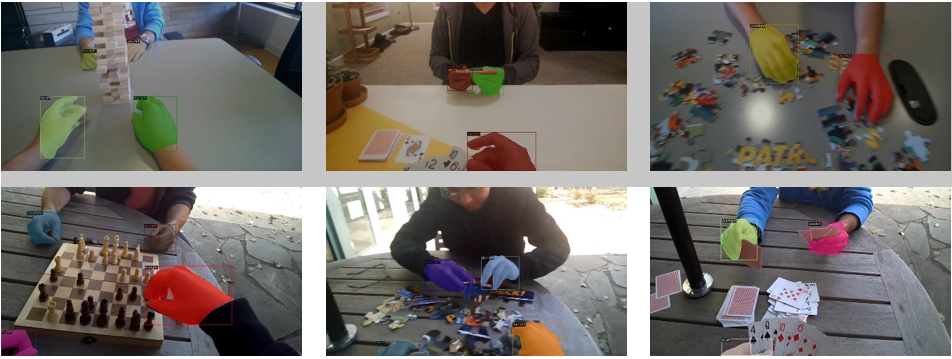
\includegraphics[width=1\linewidth]{Figs/postegohands.png}}
%	\caption{Samples from EgoHands dataset after post-processing.}
%	\label{fig:postegohands}
%\end{figure}
\subsection{Micand32 dataset} \label{subsec:micand32}
As introduced in chapter \ref{chap:intro}, the NAFOSTED’s project is carried out with the aim of using advanced deep learning techniques to evaluate the healing and surgical research of the patient with a sensor through detection segmentation, tracking, gesture recognition, and correlation of the patient's hand with objects. The members in the project prepare the script and perform data collection at Hanoi Medical Hospital. The experiment was carried out by 10 volunteers, patients aged 20 to 60 years, 5 men and 5 women under the supervision, explanation and help of doctors and instructors. The implementation site consists of 3 areas: the desk area, the sink area and the closet area. Patients will wear 5 sensors including: 1 camera at the head, 1 camera in the shoulder, 1 sensor of kinetics (sensors that will collect and store information about the carrier's position, acceleration) in the left hand, 1 kinematic sensor in the right hand, 1 kinetic sensor in the leg. The patient performs 21 agreed and pre-defined actions, such as taking stairs, practicing hands with objects, brushing hair, opening cabinets, etc. The average number of executions per action is 2. The recorded videos have very high resolution compared to the previous related datasets, is 1920x1440, frequency 30fps. Average time to perform an action is 5 seconds. Thus, in terms of images, the data set consists of 5 people x 2 cameras x 21 actions x 5 times = 1050 videos, so there will be 1050 videos x 5 seconds x 30 fps = 157500 frames.
\\The Micand32 dataset is a subset of the NAFOSTED subject dataset. In the context of the problem of detecting, partitioning and tracking human hands, this thesis is concerned with only 4/21 types of actions most relevant to the hand: (5) practice with ball, (6) practice with water bottles, (7) practice with wooden blocks, (8) practice with cylinders. Figure \ref{fig:micand32} visualizes random samples of 4 action types extracted from MICAND32.
\begin{figure}
	\centerline{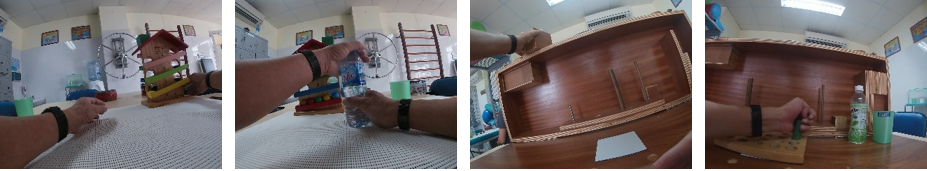
\includegraphics[width=1\linewidth]{Figs/micand32.png}}
	\caption{Randomly selected actions 5 6 7 8, from left to right respectively.}
	\label{fig:micand32}
\end{figure}
Micand32 consists of 32 sequences of 1920x1440 resolution, is divided into 2 parts: Micand32Standard includes 26 sequences and Micand32Enhanced includes 6 sequences. In particular, with Micand32Standard, each sequence contains from 100 to 300 frames, in the frames is mainly the journey of one hand doing a whole activity, this corresponds to the type of short-term tracking. This episode has lengths of each sequences that are equivalent to the MOT Challenge standards. With Micand32Enhanced, each sequence contains from 500 to 1700 frames, of which most frames contain more than 2 arms due to the intervention of the instructor's hand while the patient is performing the action. At the same time, the patient performed multiple repetitions in each sequence, corresponding to a long-term object tracking type. This episode is very close to reality, it is quite challenging and highly applicable. The ground-truth detection and partition section of this data set was labeled by 8 students using the VIA tool \cite{10.1145/3343031.3350535}. VGG Image Annotator is a simple and standalone manual annotation software for images, audio and video. VIA runs in a web browser and does not require any installation or settings. The complete VIA software fits a single independent HTML page, which is less than 400 KB in size and can be run as an offline application in most modern web browsers. Table \ref{tab:mican32Sta}, label statistical visualization and correlogram \ref{fig:micand32_visualization}  provides detailed statistics on Micand32: 1 category, 11k images, 18k instances, 2 instances/images. The hands highly present at the edge of frame, the size of the hands are various. 
\begin{table}[]
	\centering
	\label{tab:mican32Sta}
	\caption{Detailed enumeration of the Micand32 dataset.}
	\begin{tabular}{|l|l|l|l|l|}
		\hline
		\textbf{No} & Name                         & Action   Type & \begin{tabular}[c]{@{}l@{}}Numbers\\ of frames\end{tabular} & \begin{tabular}[c]{@{}l@{}}Hand/\\ Frame\end{tabular} \\ \hline
		1           & GH010354\_7\_13210\_16534    & 7             & 120                                                         & 1                                                     \\ \hline
		2           & GH010354\_7\_16605\_17602\_1 & 7             & 130                                                         & 1                                                     \\ \hline
		3           & GH010354\_7\_16605\_17602\_2 & 7             & 120                                                         & 1                                                     \\ \hline
		4           & GH010354\_8\_26079\_29031    & 8             & 191                                                         & 1                                                     \\ \hline
		5           & GH010358\_7\_2490\_3390\_1   & 7             & 160                                                         & 1                                                     \\ \hline
		6           & GH010358\_7\_2490\_3390\_2   & 7             & 160                                                         & 1                                                     \\ \hline
		7           & GH010358\_7\_352\_2464\_1    & 7             & 110                                                         & 1                                                     \\ \hline
		8           & GH010358\_7\_352\_2464\_2    & 7             & 135                                                         & 1                                                     \\ \hline
		9           & GH010374\_6\_4944\_6241\_1   & 6             & 140                                                         & 1                                                     \\ \hline
		10          & GH010374\_6\_4944\_6241\_1   & 6             & 100                                                         & 1                                                     \\ \hline
		11          & GH010382\_5\_5725\_7093\_1   & 5             & 100                                                         & 1                                                     \\ \hline
		12          & GH010382\_5\_5725\_7093\_2   & 5             & 130                                                         & 1                                                     \\ \hline
		13          & GH010382\_5\_955\_4771\_1    & 5             & 115                                                         & 1                                                     \\ \hline
		14          & GH010382\_5\_955\_4771\_2    & 5             & 115                                                         & 1                                                     \\ \hline
		15          & GH010382\_6\_18190\_20215\_1 & 6             & 151                                                         & 1                                                     \\ \hline
		16          & GH010382\_6\_18190\_20215\_2 & 6             & 150                                                         & 1                                                     \\ \hline
		17          & GH010382\_6\_20592\_21726\_1 & 6             & 90                                                          & 1                                                     \\ \hline
		18          & GH010382\_6\_20592\_21726\_2 & 6             & 125                                                         & 1                                                     \\ \hline
		19          & GH010382\_8\_16207\_17479\_1 & 8             & 100                                                         & 1                                                     \\ \hline
		20          & GH010382\_8\_16207\_17479\_2 & 8             & 100                                                         & 1                                                     \\ \hline
		21          & GH010383\_5\_462\_968\_1     & 5             & 100                                                         & 1                                                     \\ \hline
		22          & GH010383\_5\_462\_968\_2     & 5             & 120                                                         & 1                                                     \\ \hline
		23          & GH010383\_8\_3221\_3956\_1   & 8             & 100                                                         & 1                                                     \\ \hline
		24          & GH010383\_8\_3221\_3956\_1   & 8             & 100                                                         & 1                                                     \\ \hline
		25          & GH010383\_8\_4544\_5192\_1   & 8             & 100                                                         & 1                                                     \\ \hline
		26          & GH010383\_8\_4544\_5192\_2   & 8             & 100                                                         & 1                                                     \\ \hline
		& MICAND32Standard             & 5, 6, 7,   8  & \textbf{3162}                                               & 1                                                     \\ \hline
		27          & GH010354\_5\_17718\_19366    & 5             & 1684                                                        & 1                                                     \\ \hline
		28          & GH010373\_5\_1284\_2724      & 5             & 1440                                                        & 5                                                     \\ \hline
		29          & GH010358\_6\_10208\_11900    & 6             & 1594                                                        & 4                                                     \\ \hline
		30          & GH010373\_6\_3150\_4744      & 6             & 1692                                                        & 6                                                     \\ \hline
		31          & GH010358\_7\_2490\_3390      & 7             & 900                                                         & 4                                                     \\ \hline
		32          & GH010358\_8\_8000\_8547      & 8             & 547                                                         & 3                                                     \\ \hline
		& MICAND32Enhanced             & 5, 6, 7,   8  & \textbf{7857}                                               & 4                                                     \\ \hline
		& MICAND32                     & 5, 6, 7,   8  & \textbf{11019}                                              & 2                                                     \\ \hline
	\end{tabular}
\end{table}
\\In order to evaluate the effectiveness of the tracking algorithm, there is currently no standard popular tool to support the id tag of the object in the video frame. To the best of my knowledge, currently there is no egocentric dataset that involves detailed standard for hand tracking, according to \cite{9064606}. This thesis refers to the MOT Challenge tracking data standard and the annotator has done the tracking tagging through a self-developed tool called EHTA. Egocentric Hand Tracking Annotator was especially designed to model semi-automatic annotation pipelines to speed up the annotation process. Such a semi-automatic can be achieved by using AI generated annotation proposals that are presented to an annotator inside the annotation tool. Also, EHTA integrates a part of the VIA labeling tool \cite{10.1145/3343031.3350535}.
Figure \ref{fig:micand32Trajectory} performs trajectory of the patient’s hands opening water bottle, in which the groundtruth is visualized by EHTA.
\begin{figure*}[ht!]
	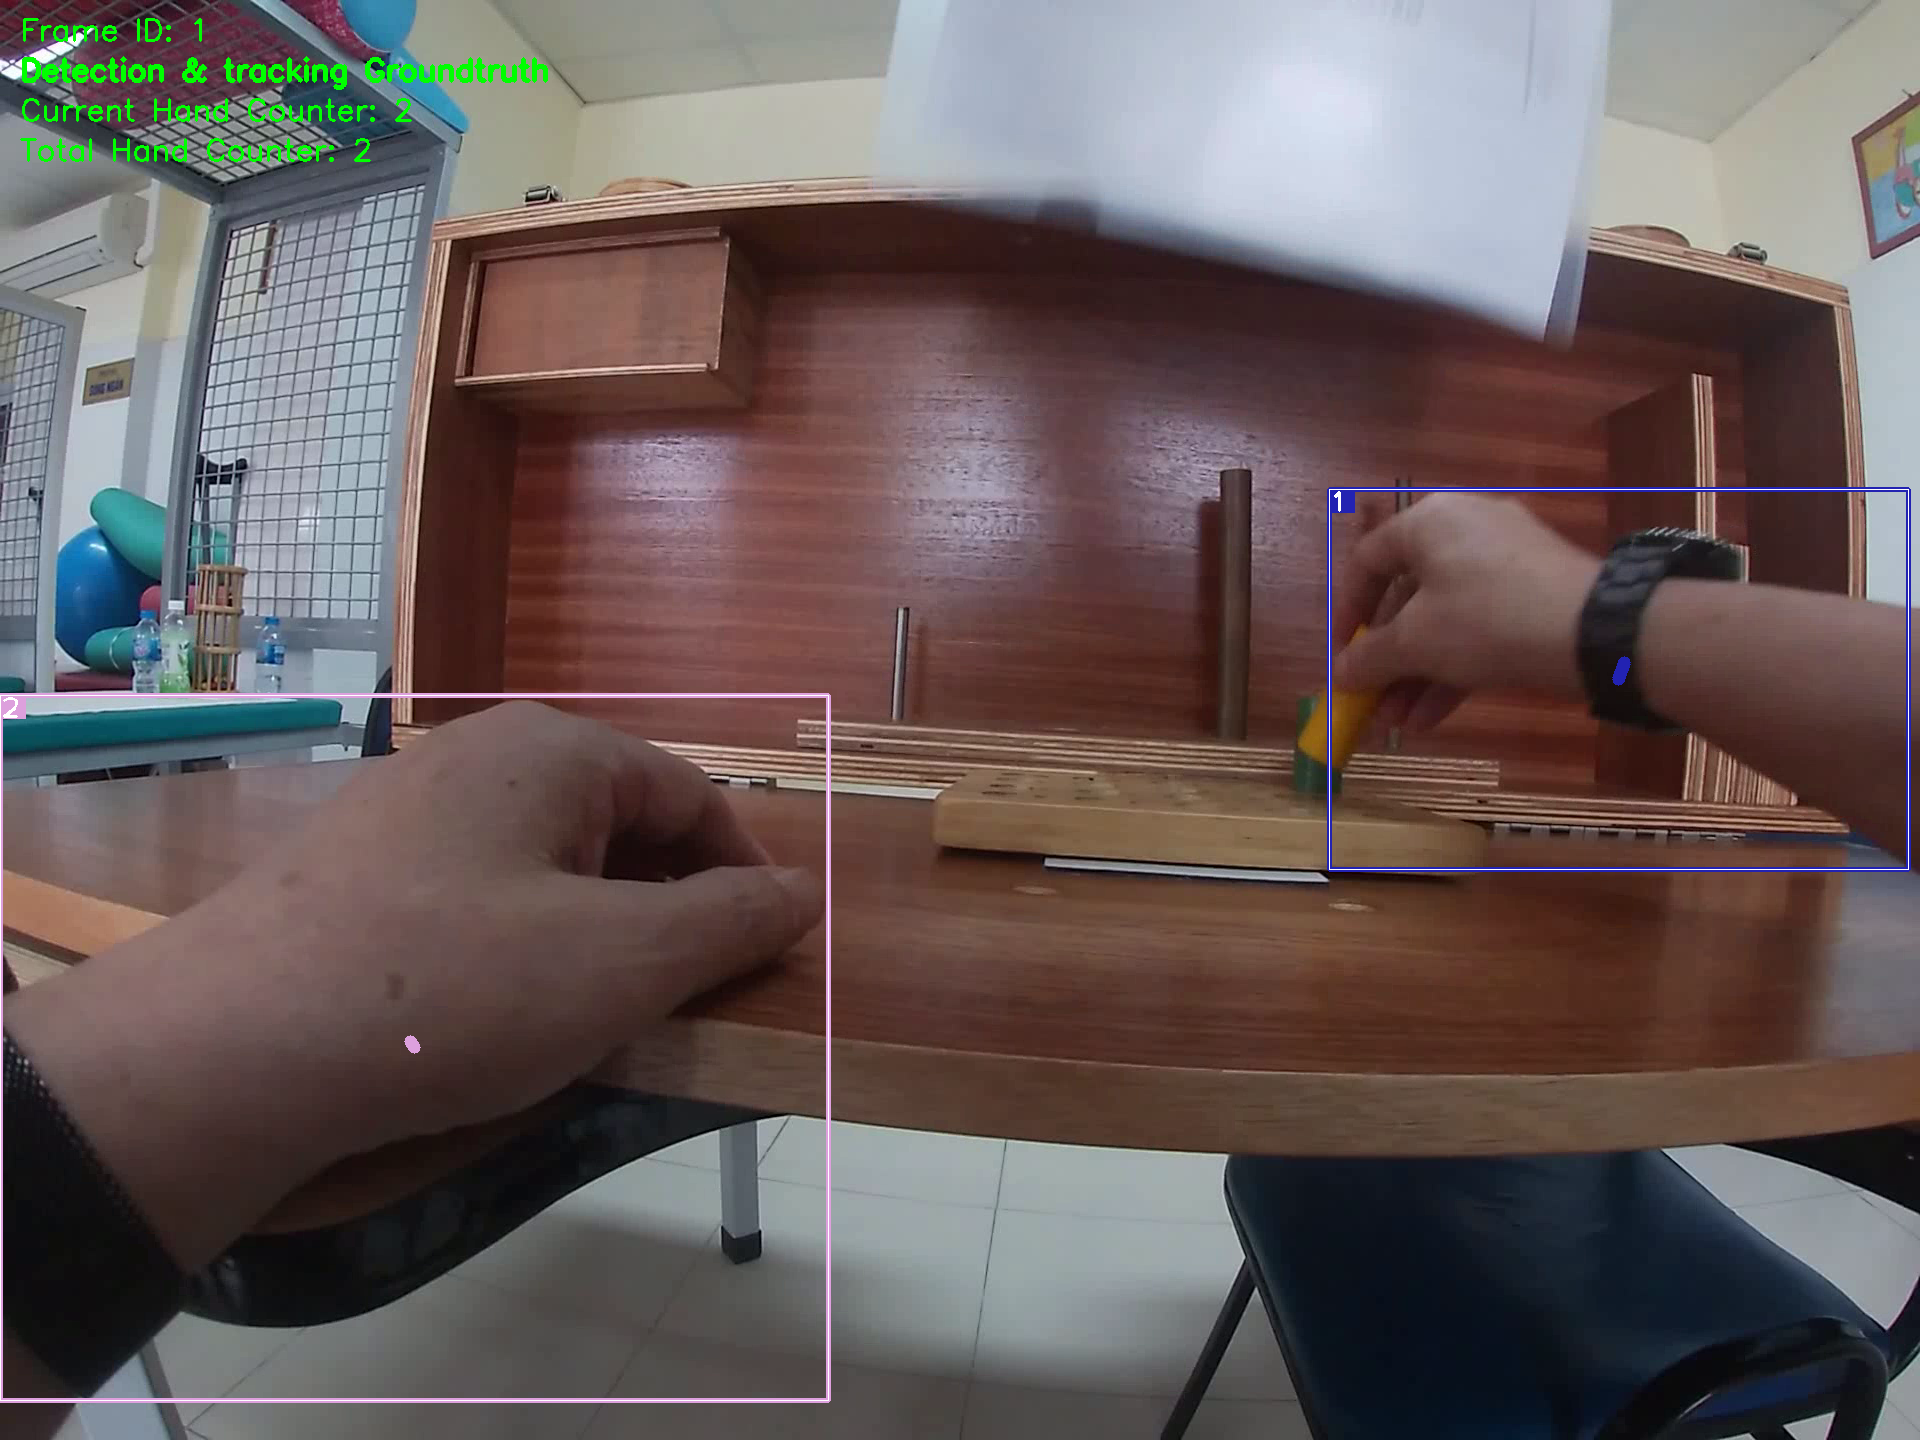
\includegraphics[width=.12\textwidth]{Figs/trajectory/1.png}\hfill
	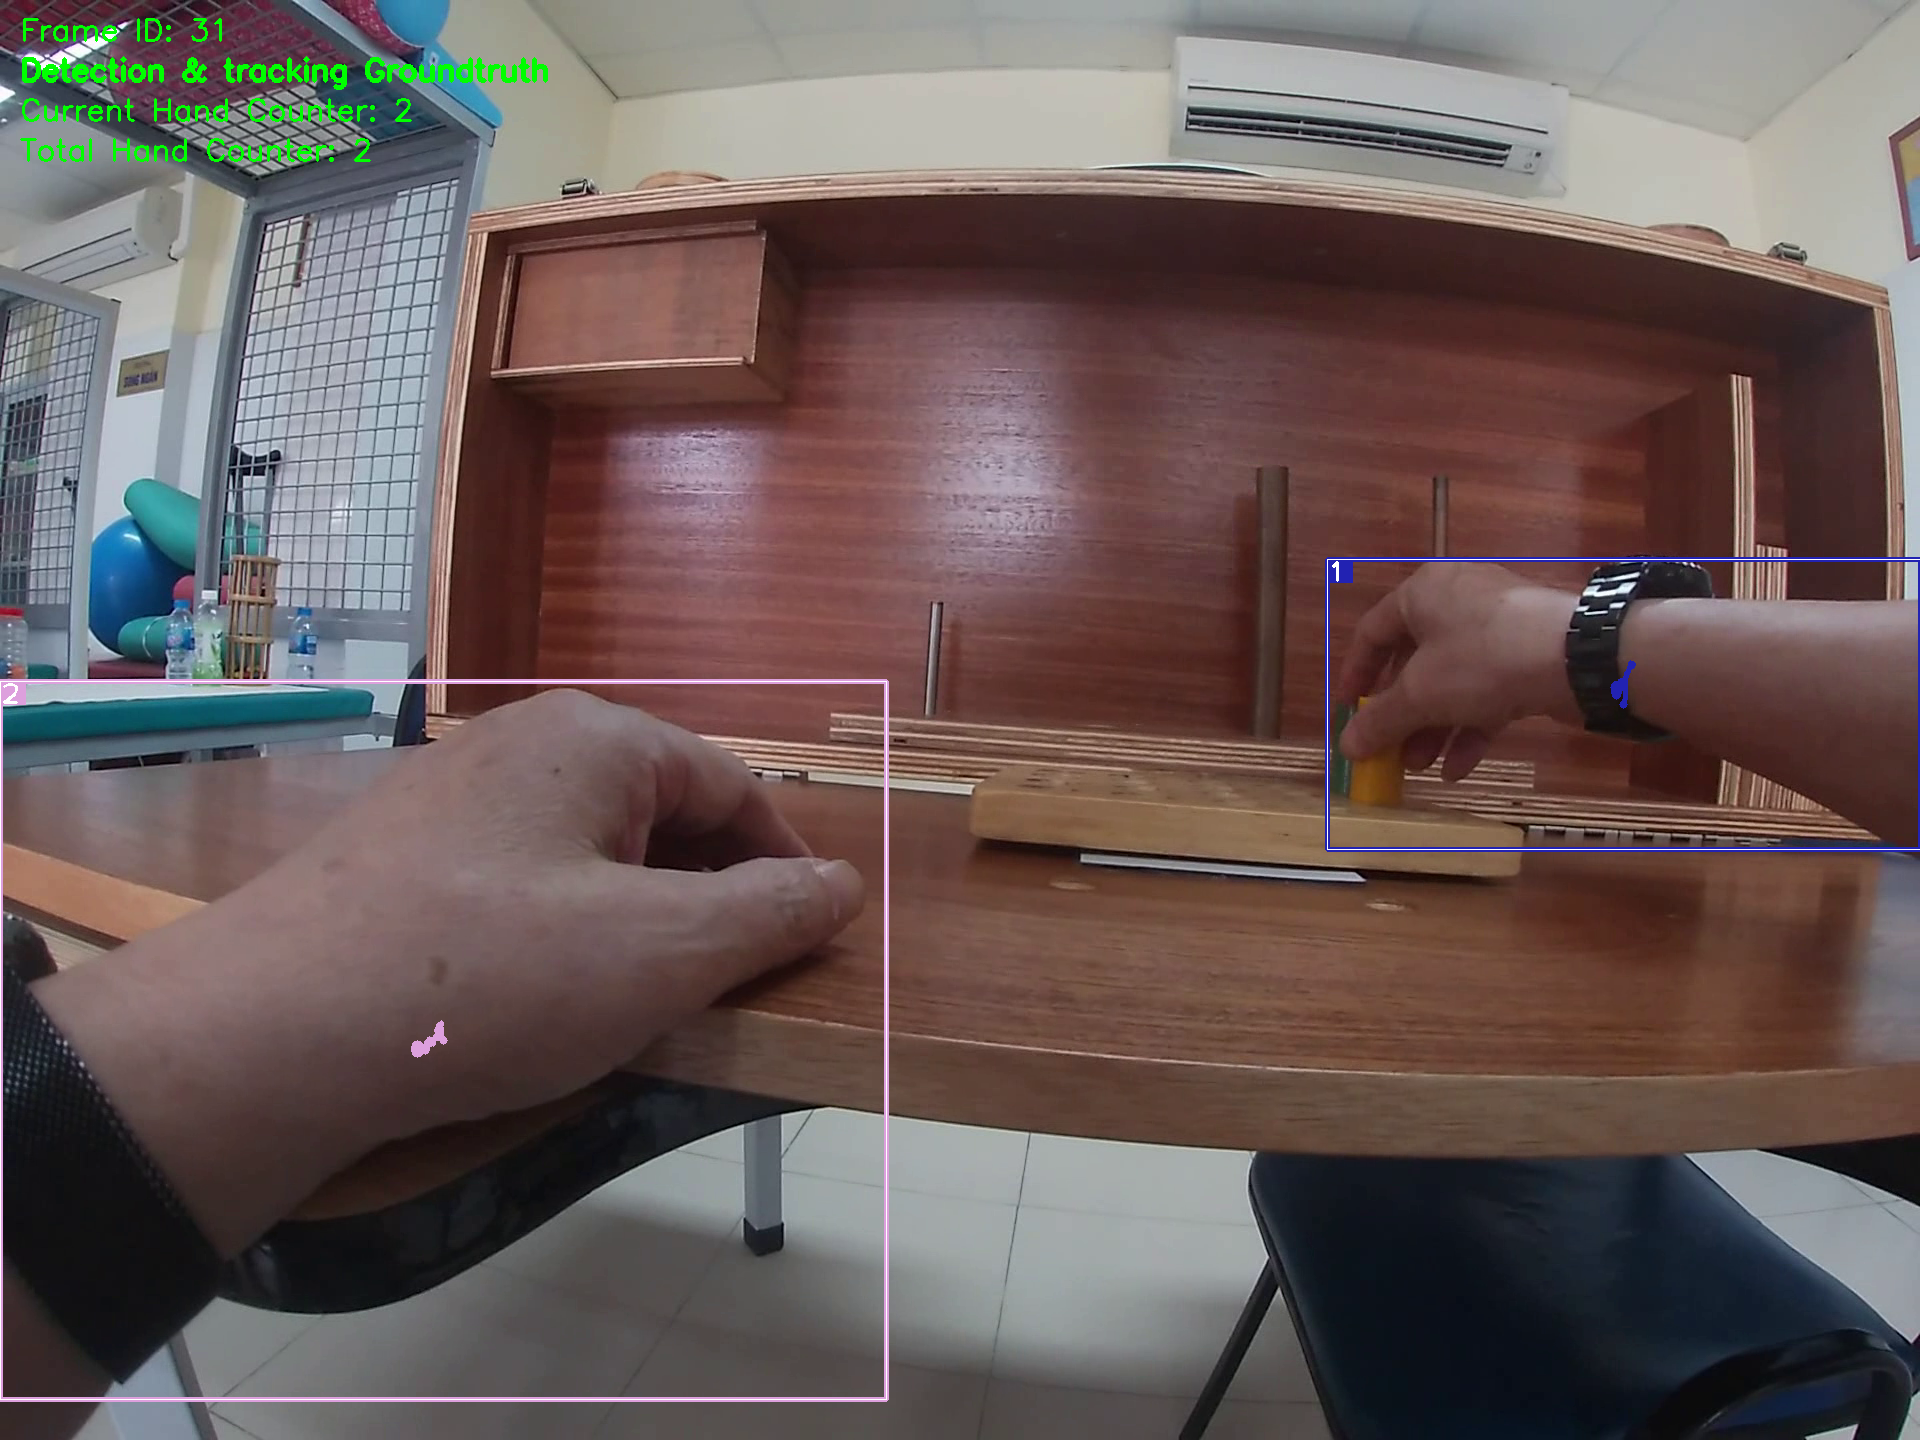
\includegraphics[width=.12\textwidth]{Figs/trajectory/31.png}\hfill	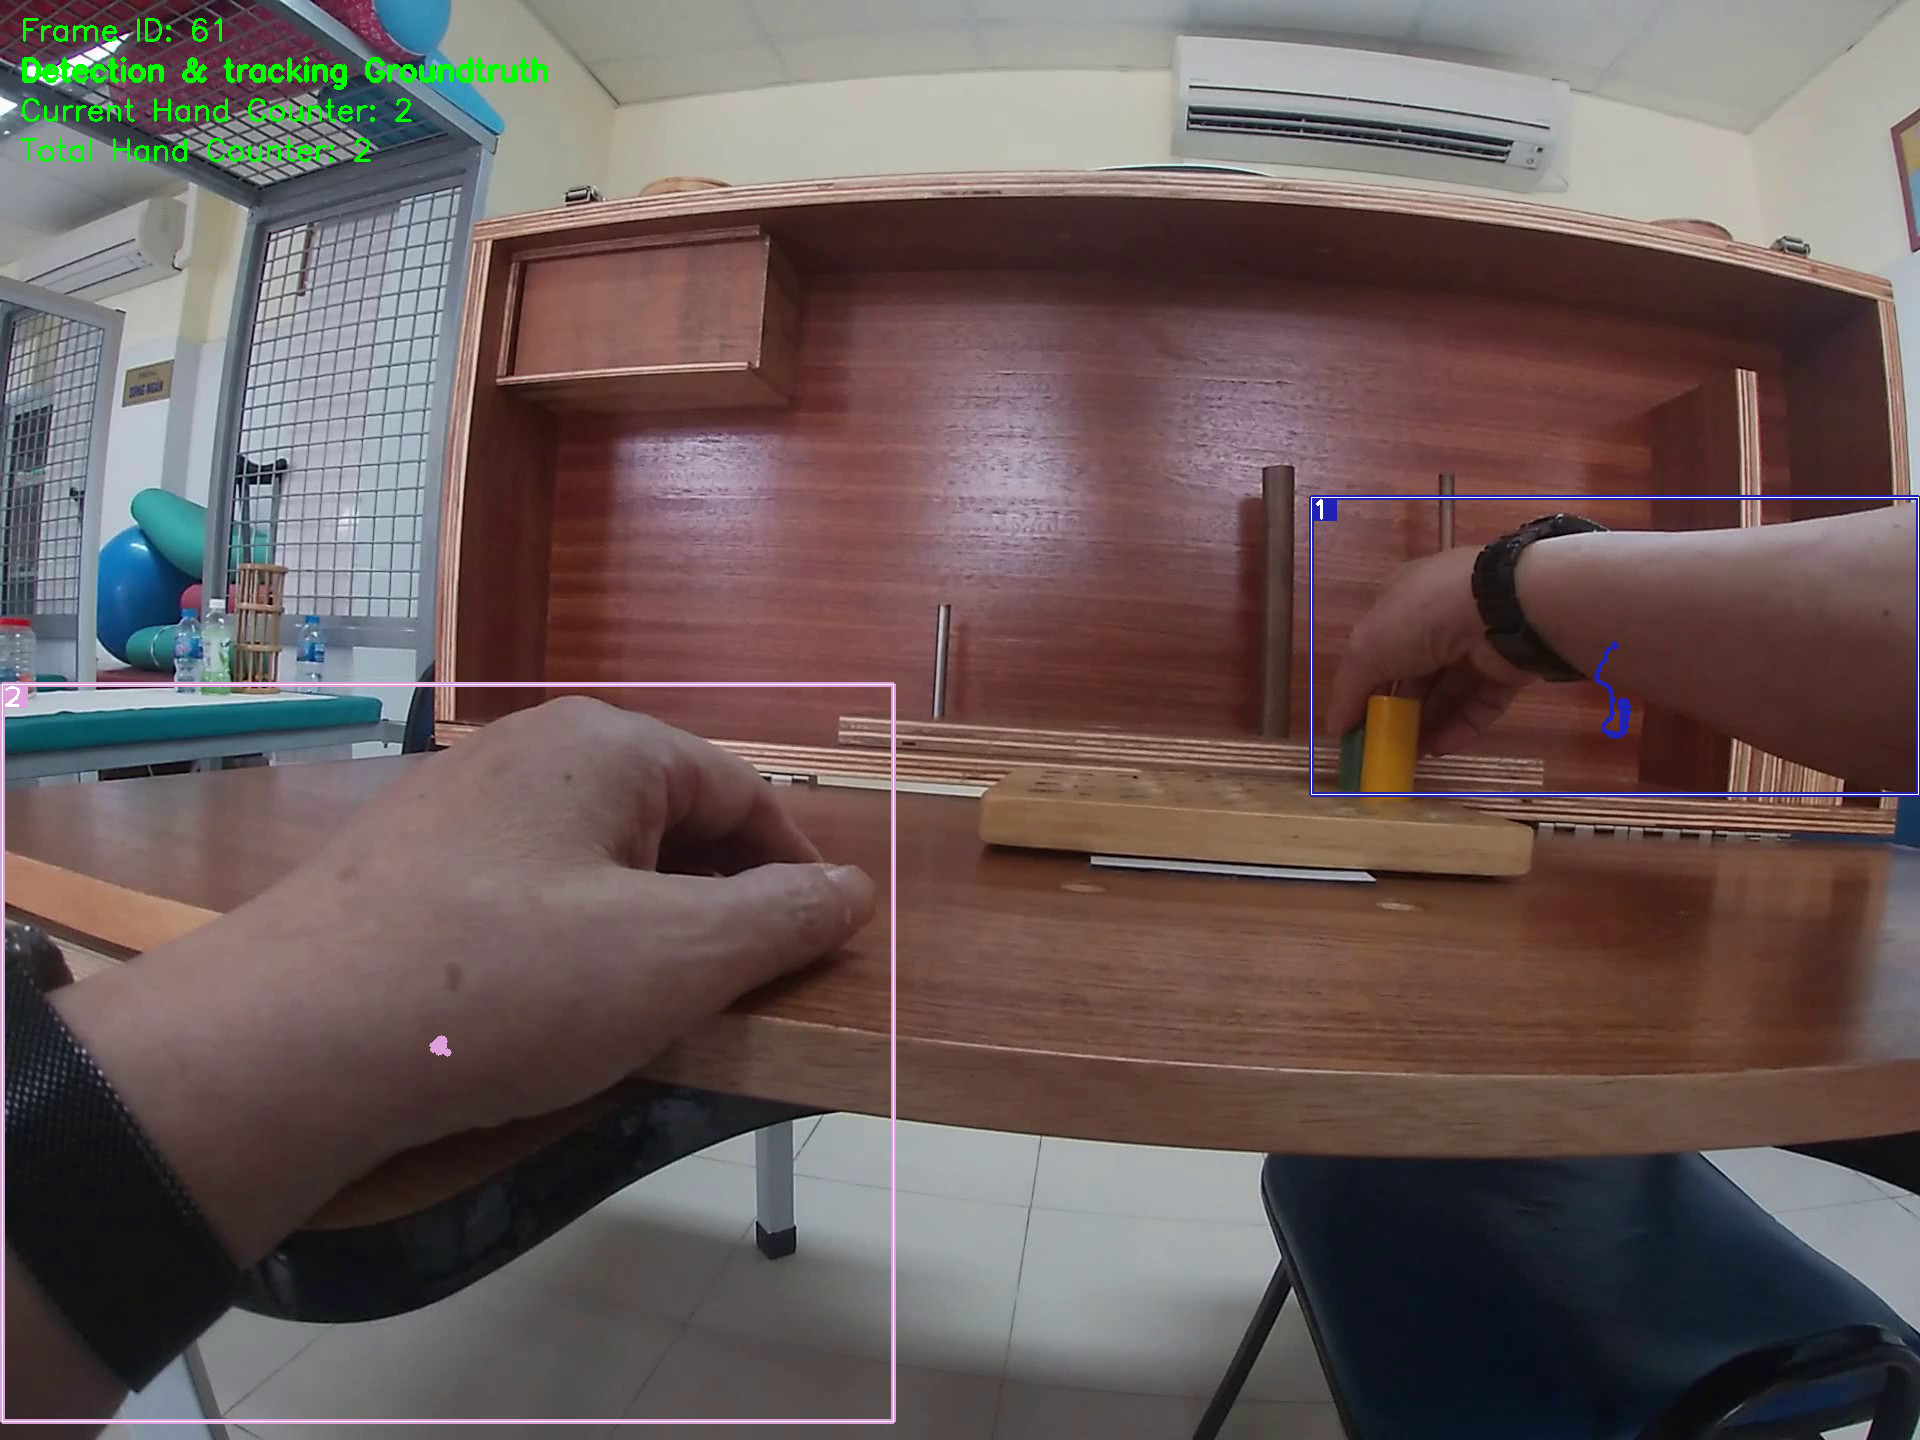
\includegraphics[width=.12\textwidth]{Figs/trajectory/61.png}\hfill
	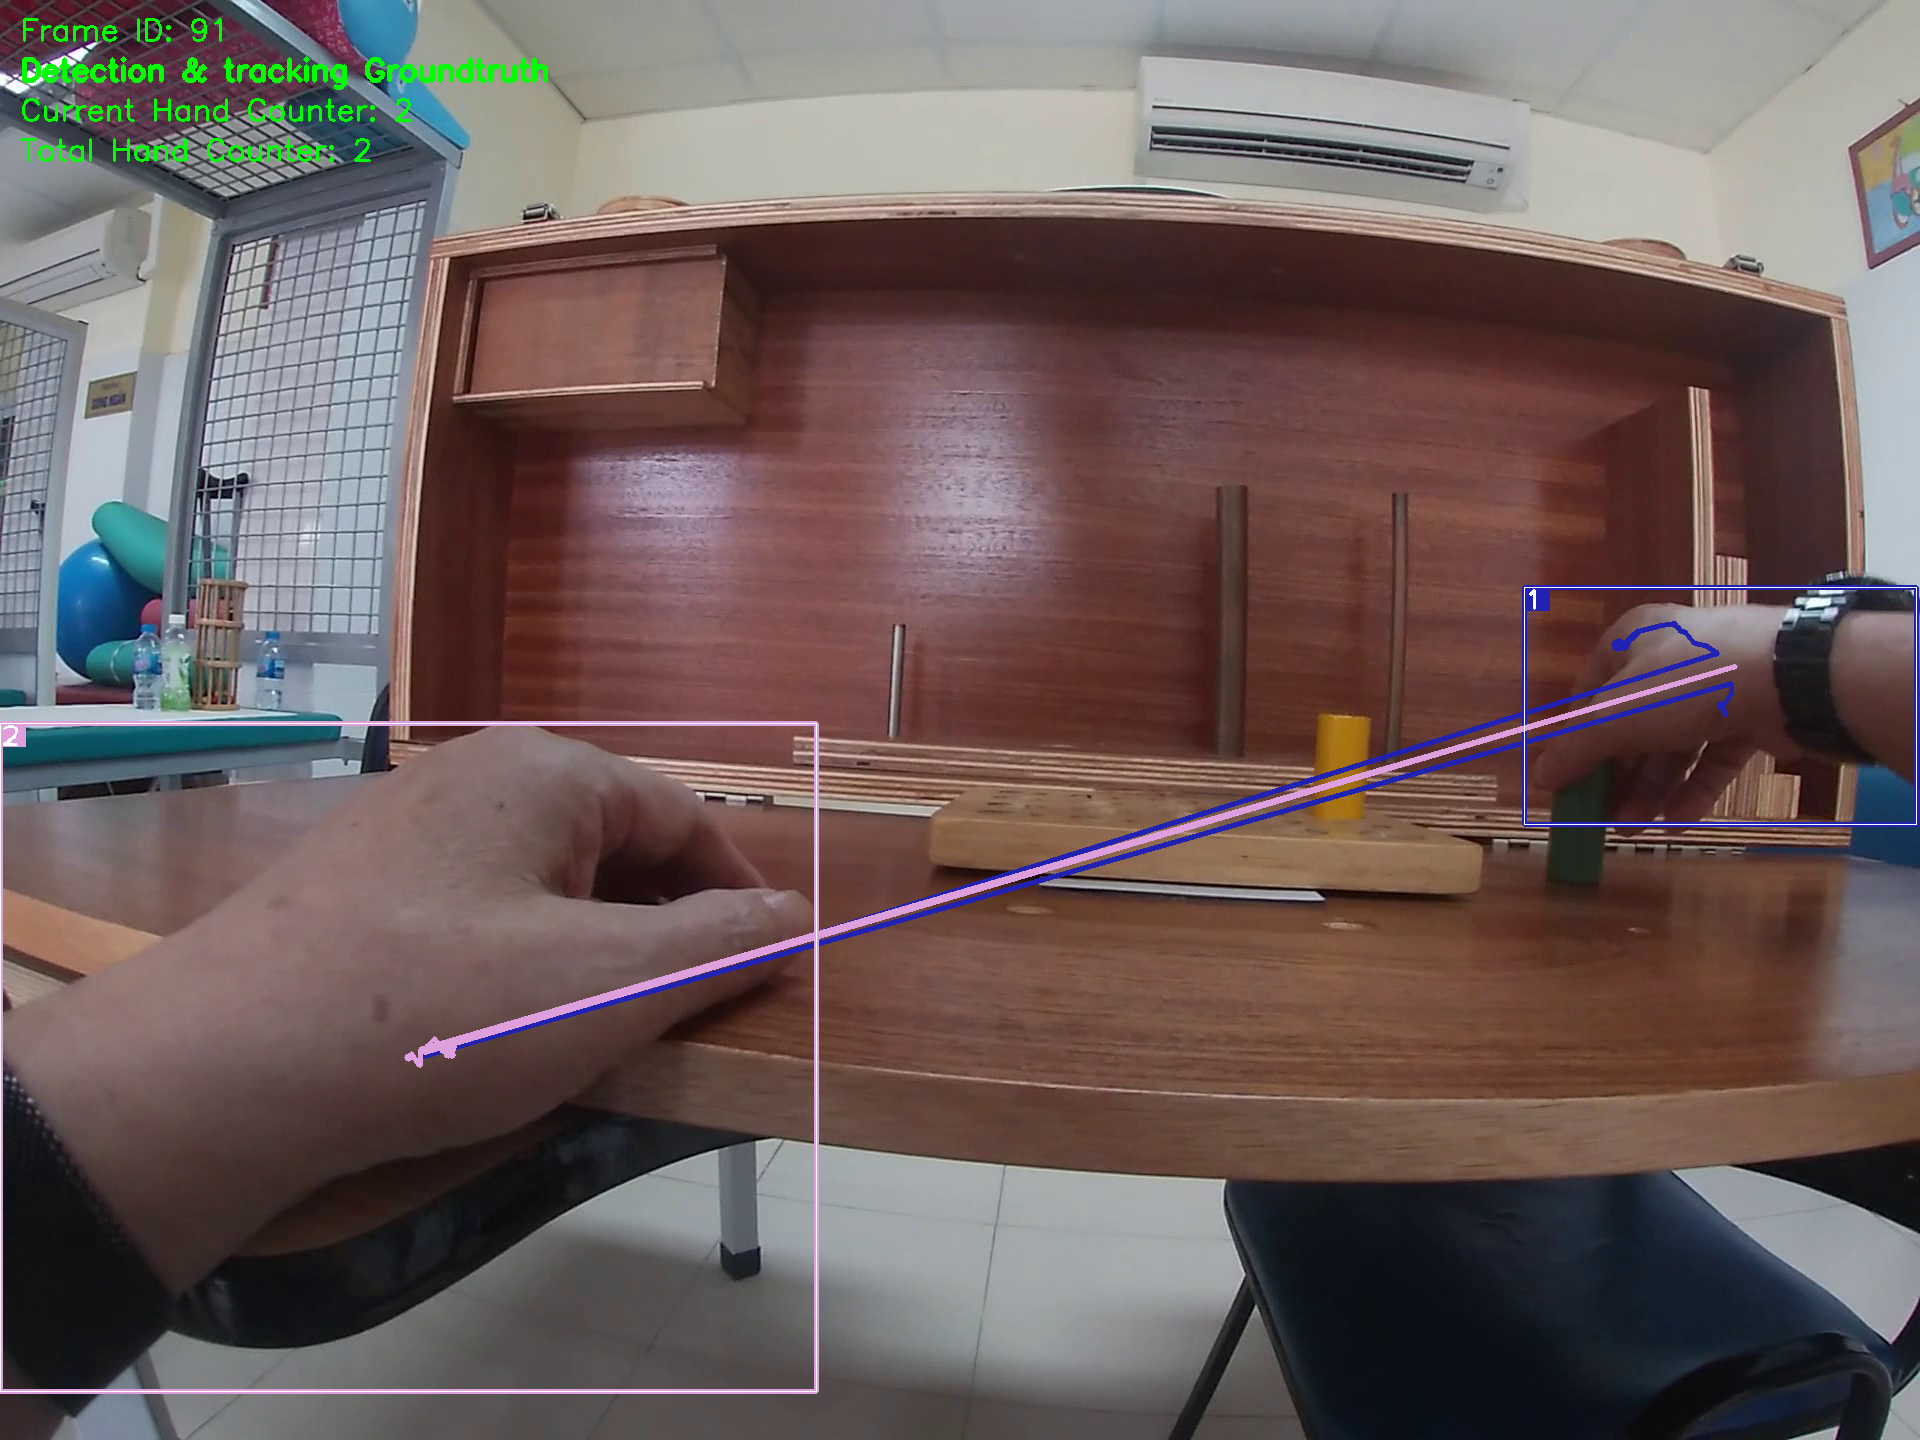
\includegraphics[width=.12\textwidth]{Figs/trajectory/91.png}\hfill	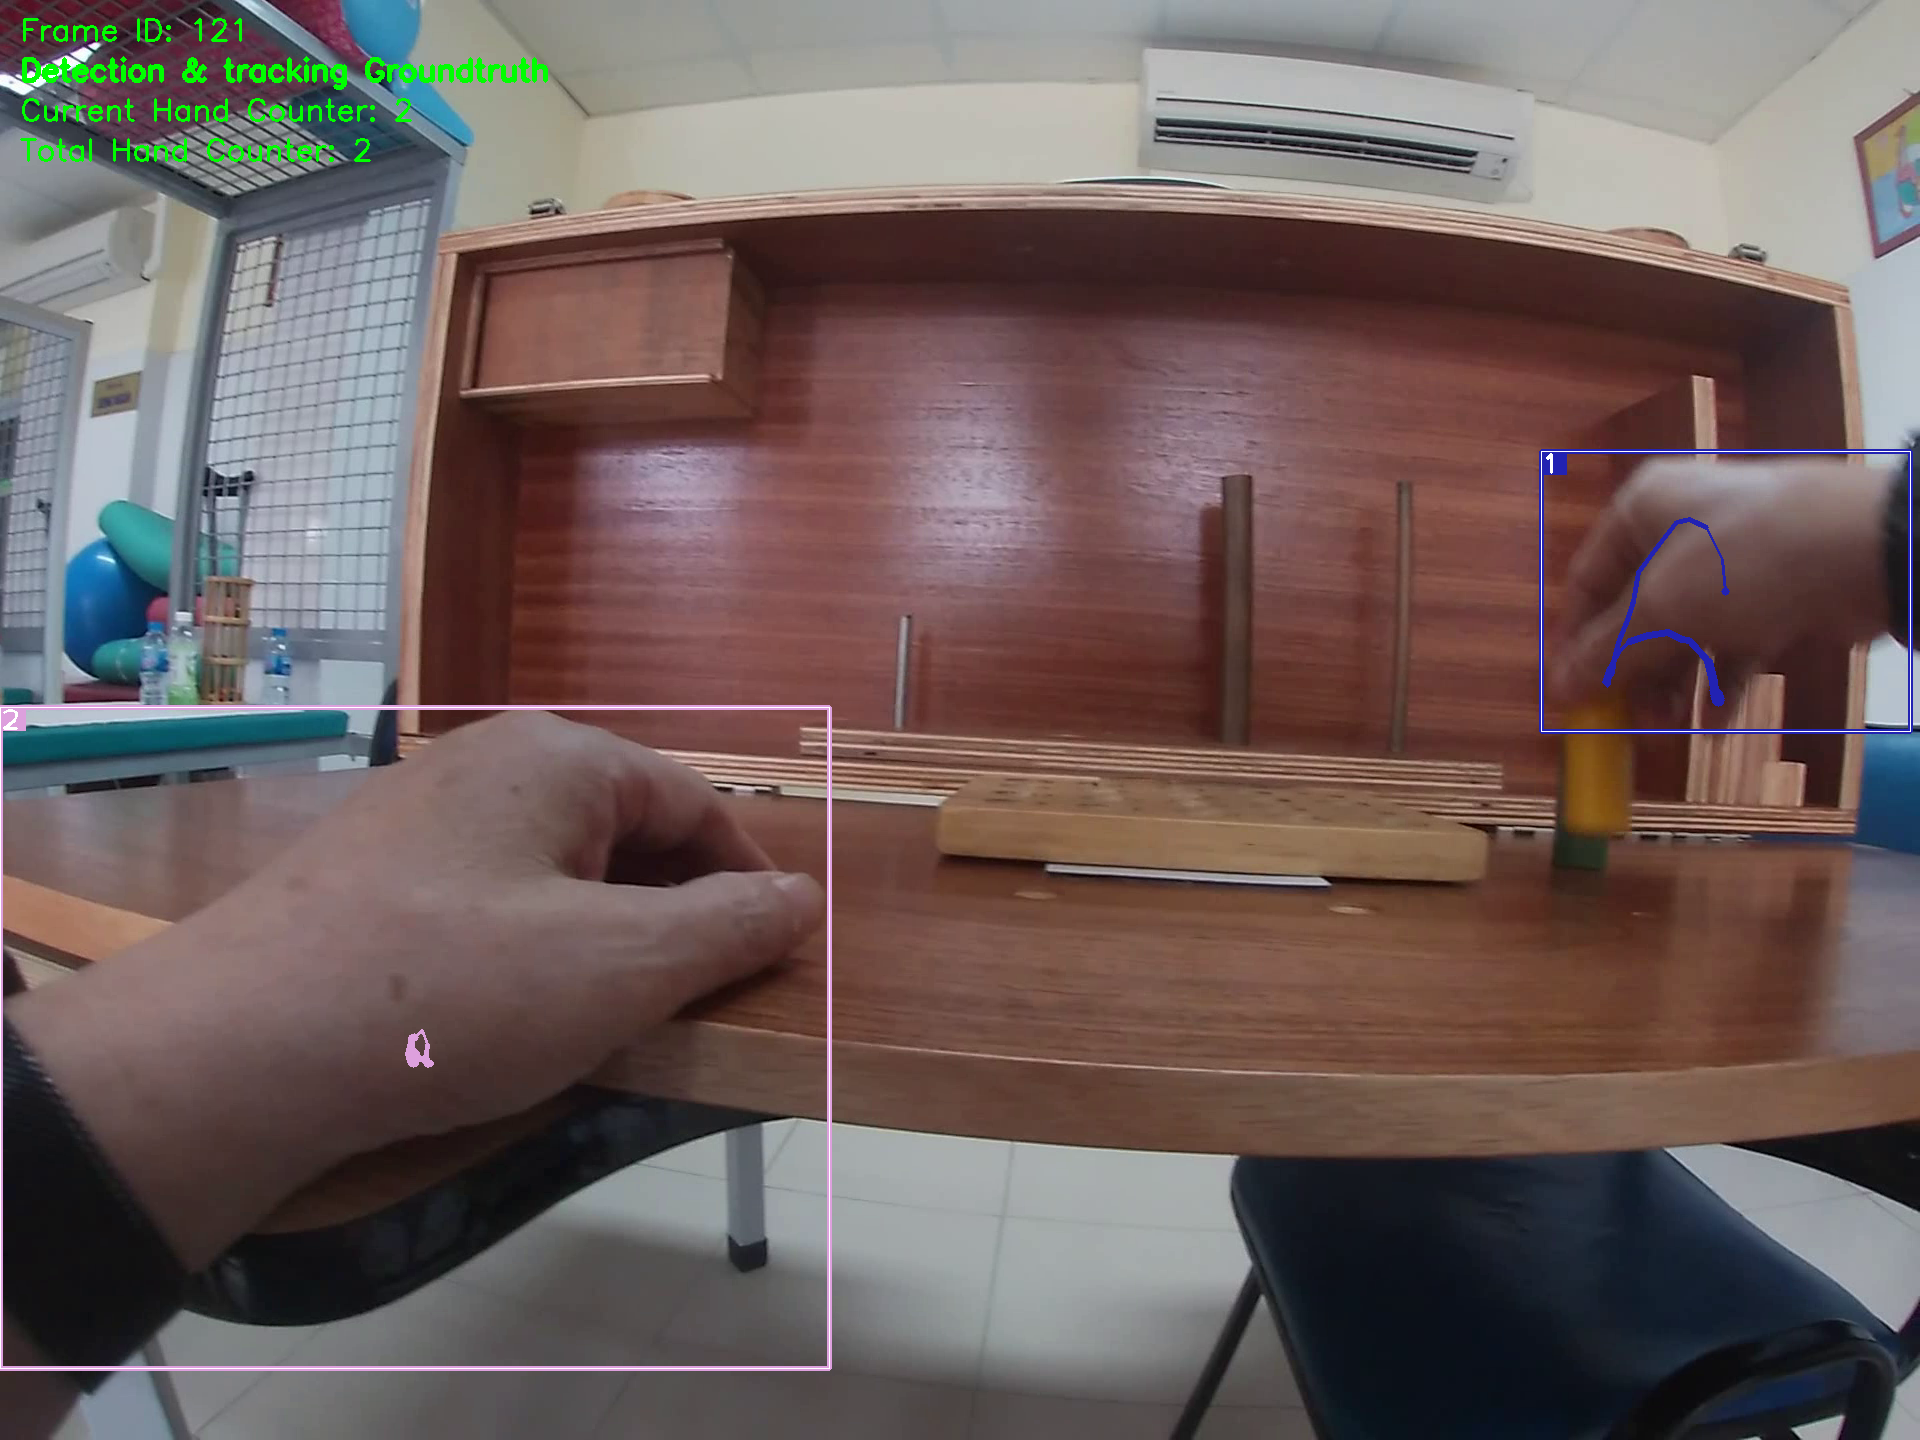
\includegraphics[width=.12\textwidth]{Figs/trajectory/121.png}\hfill
	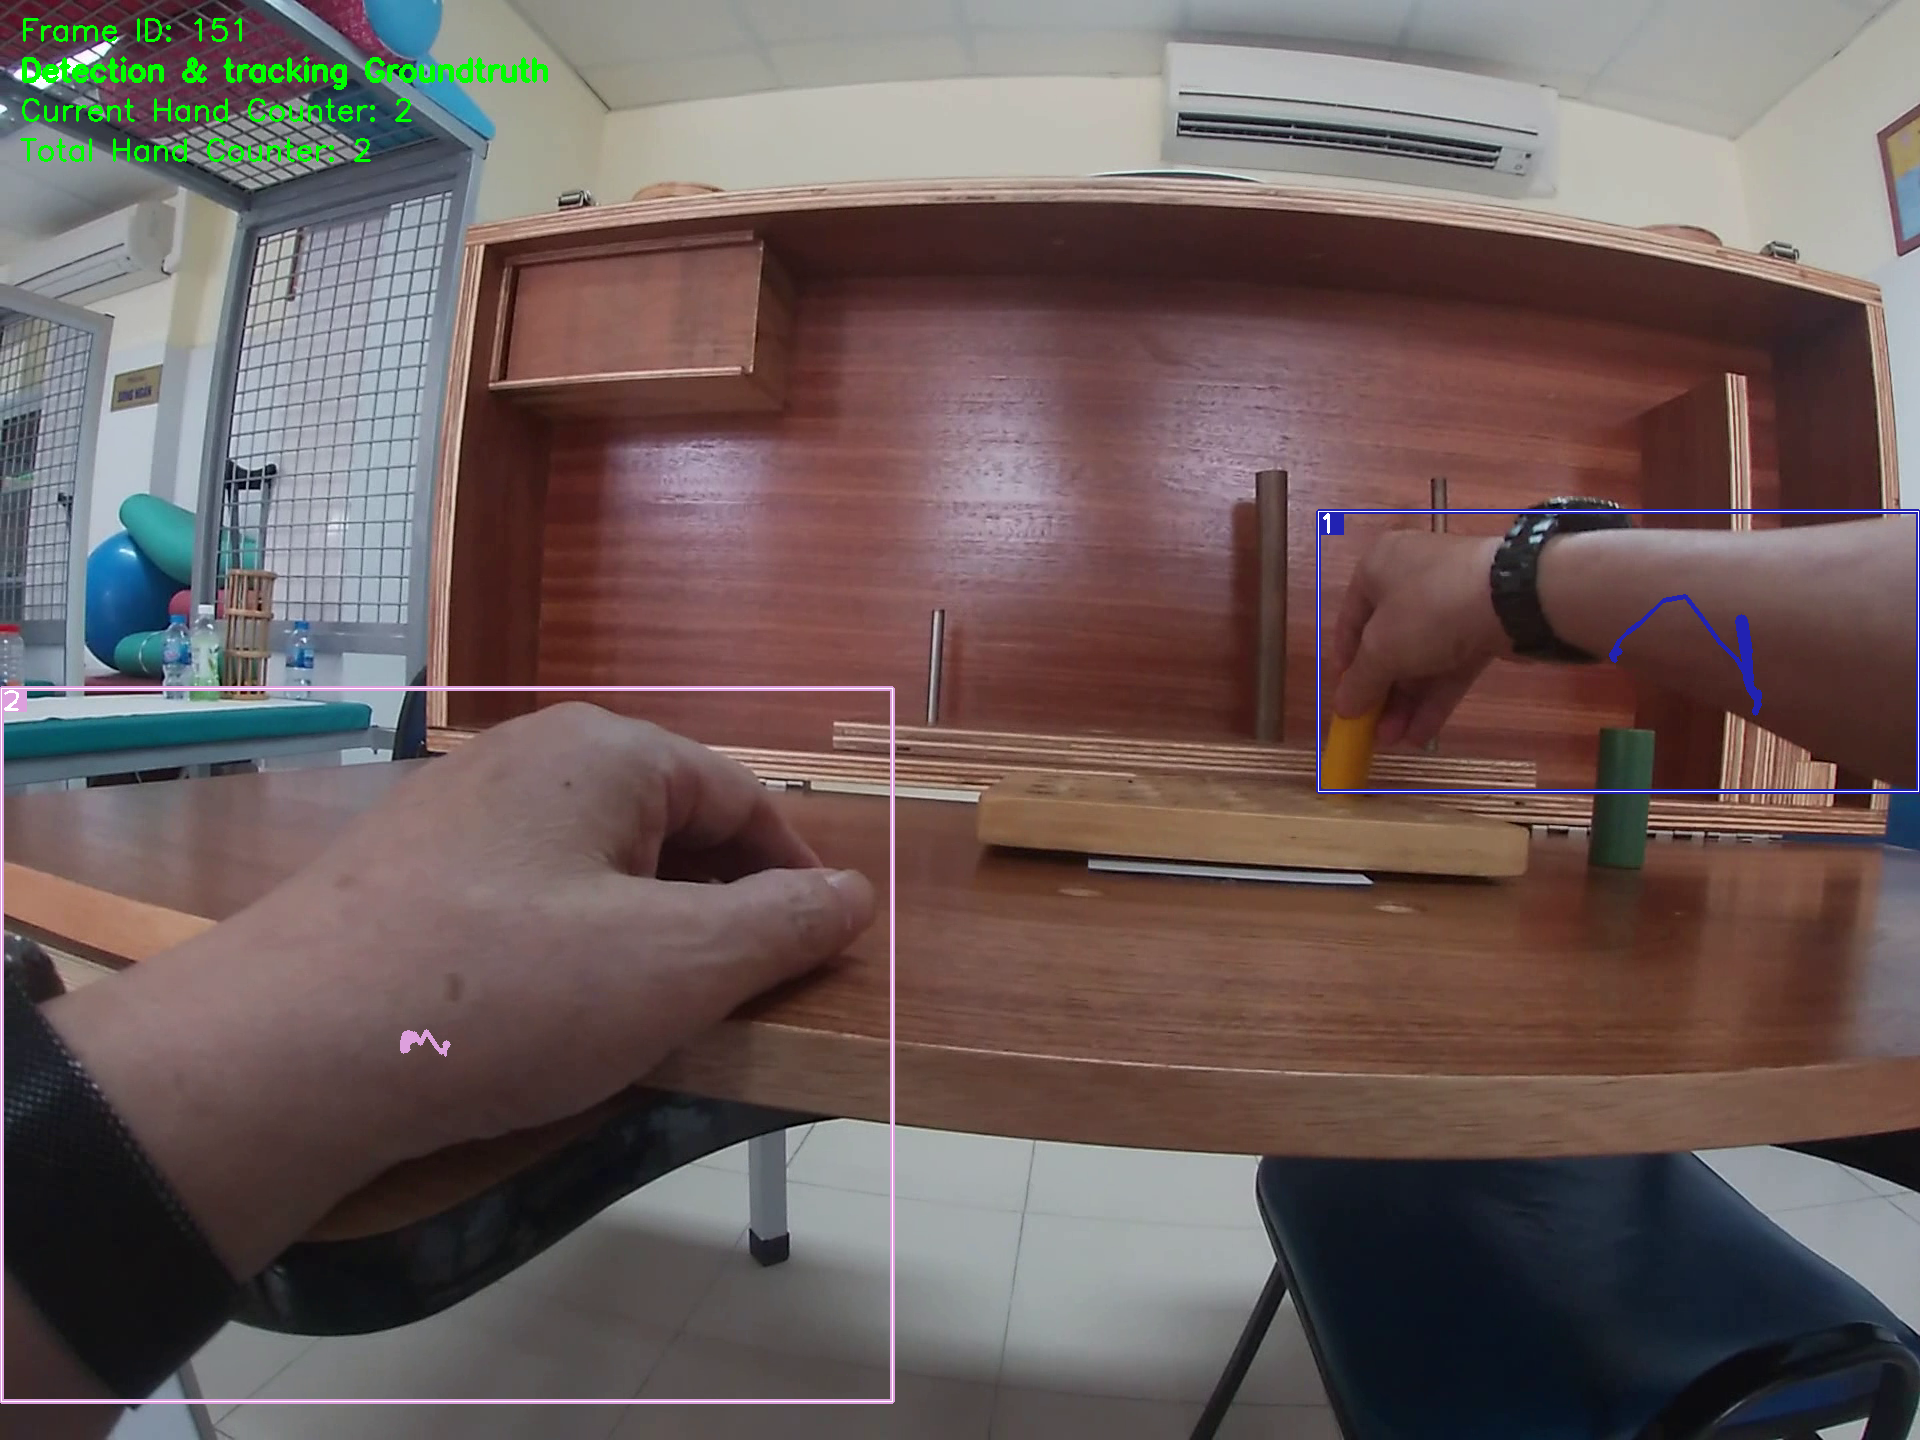
\includegraphics[width=.12\textwidth]{Figs/trajectory/151.png}\hfill
	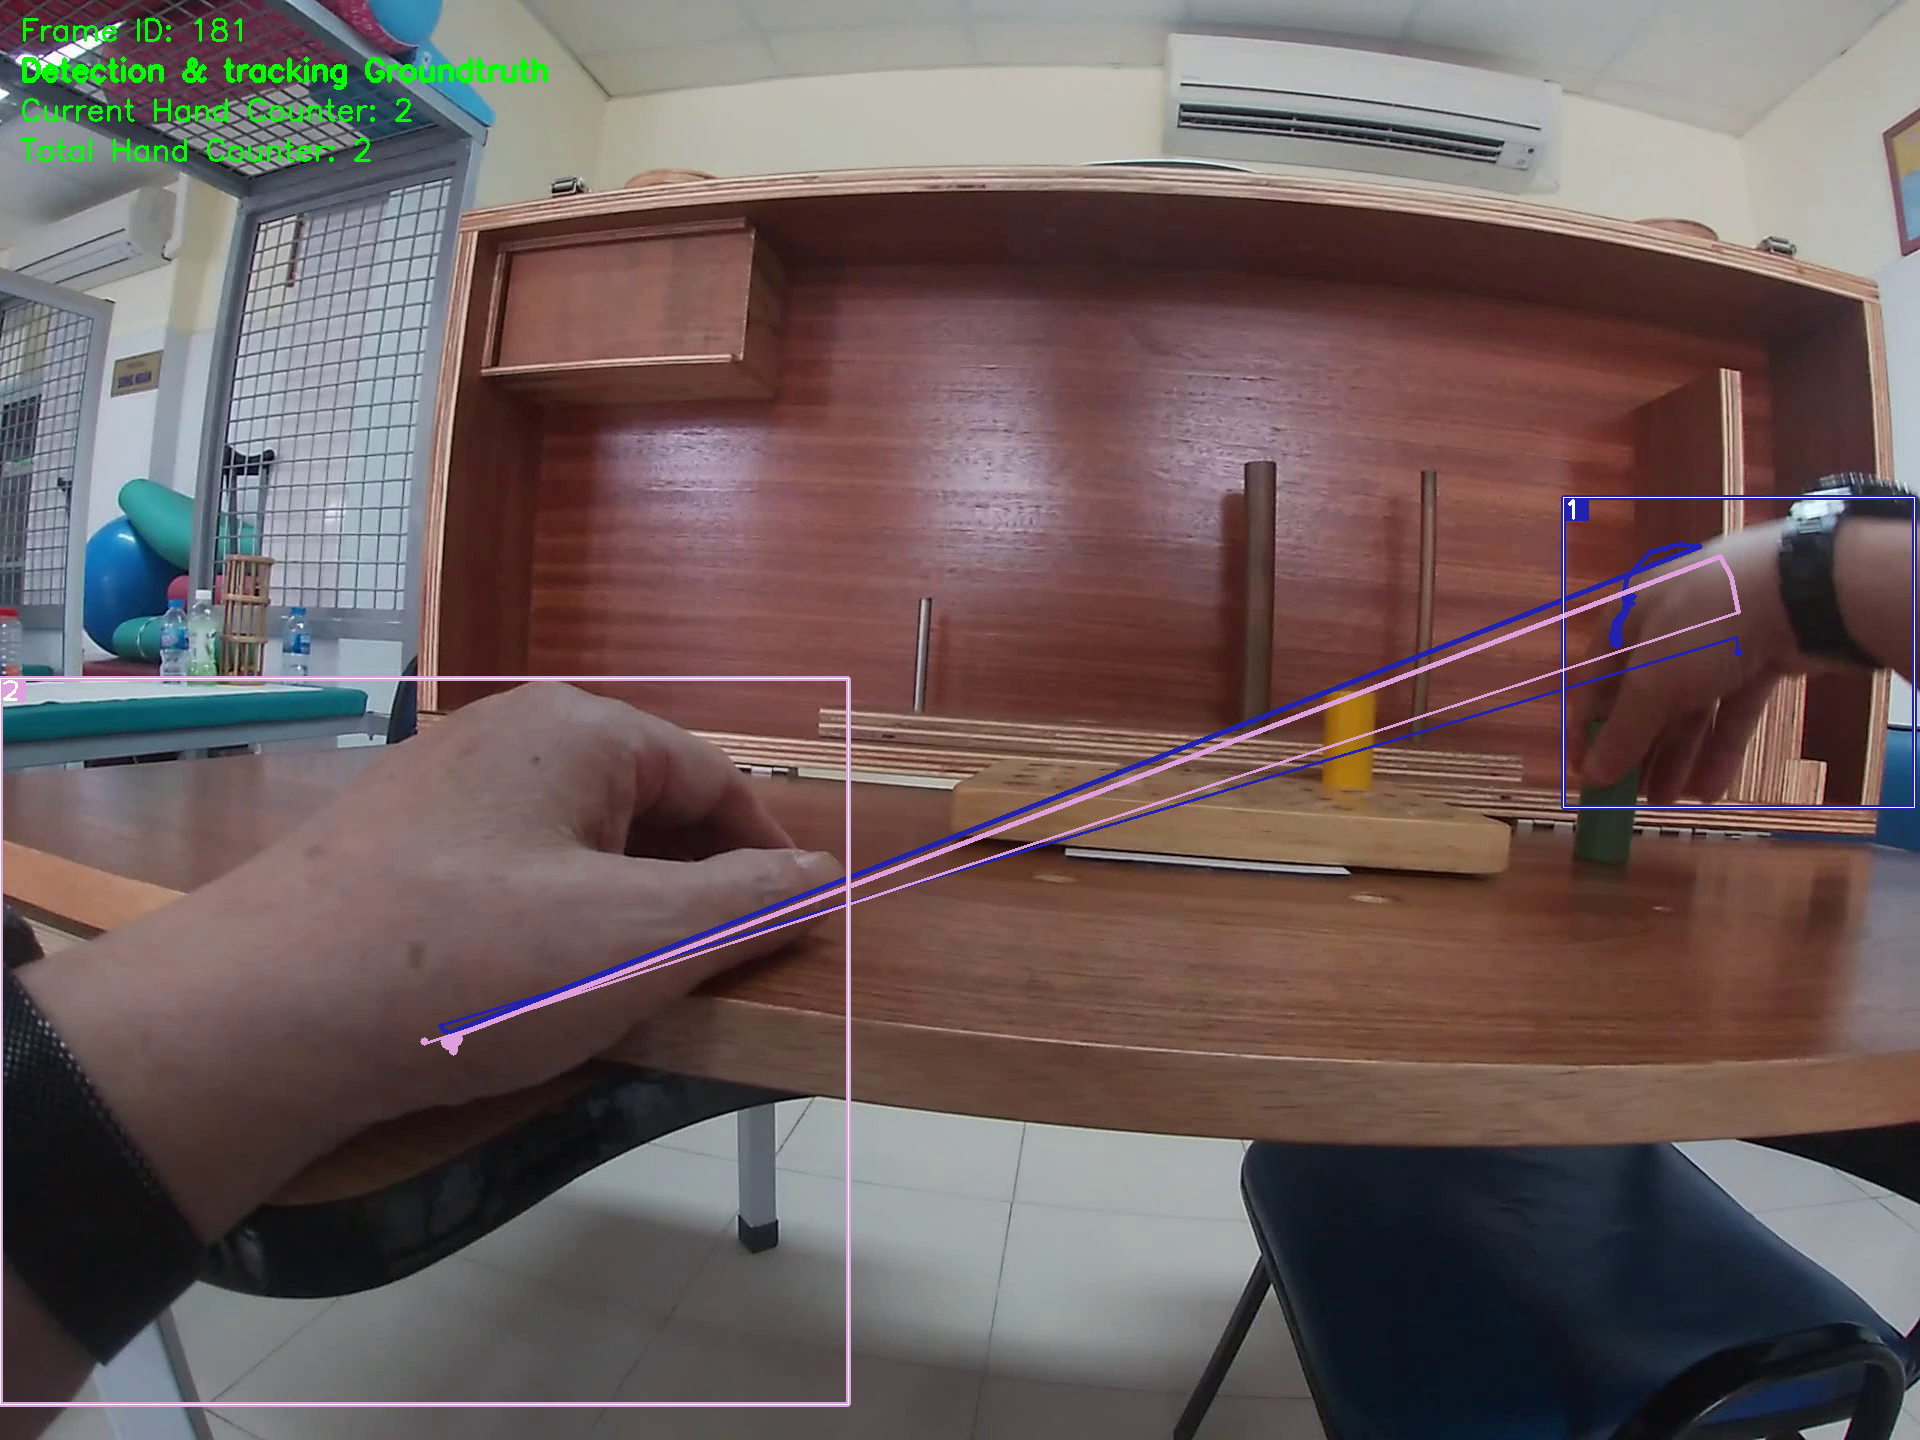
\includegraphics[width=.12\textwidth]{Figs/trajectory/181.png}\hfill
	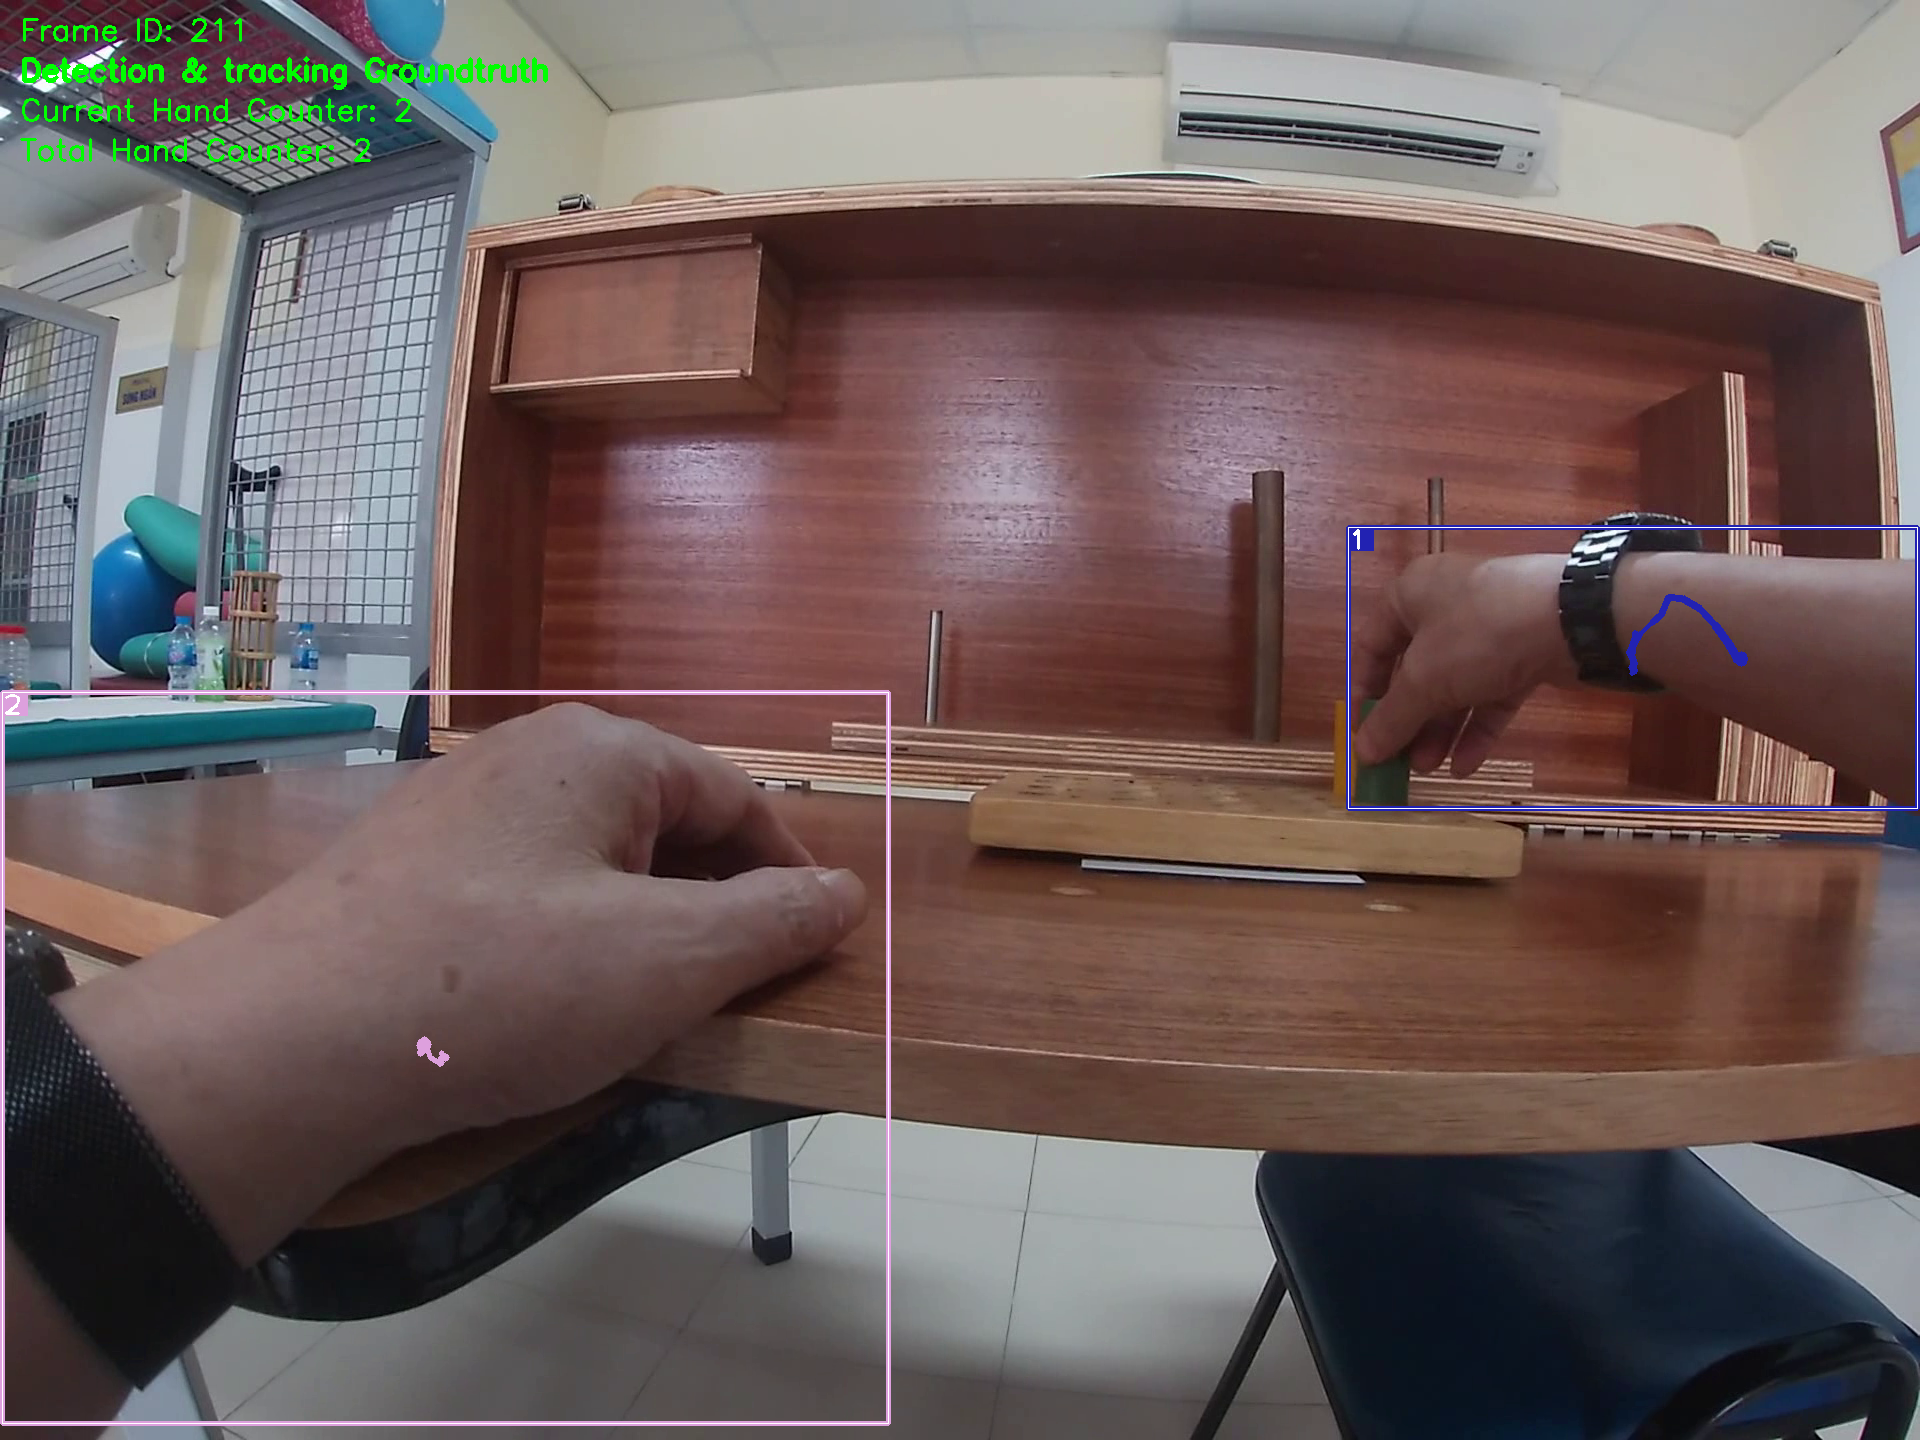
\includegraphics[width=.12\textwidth]{Figs/trajectory/211.png}\hfill	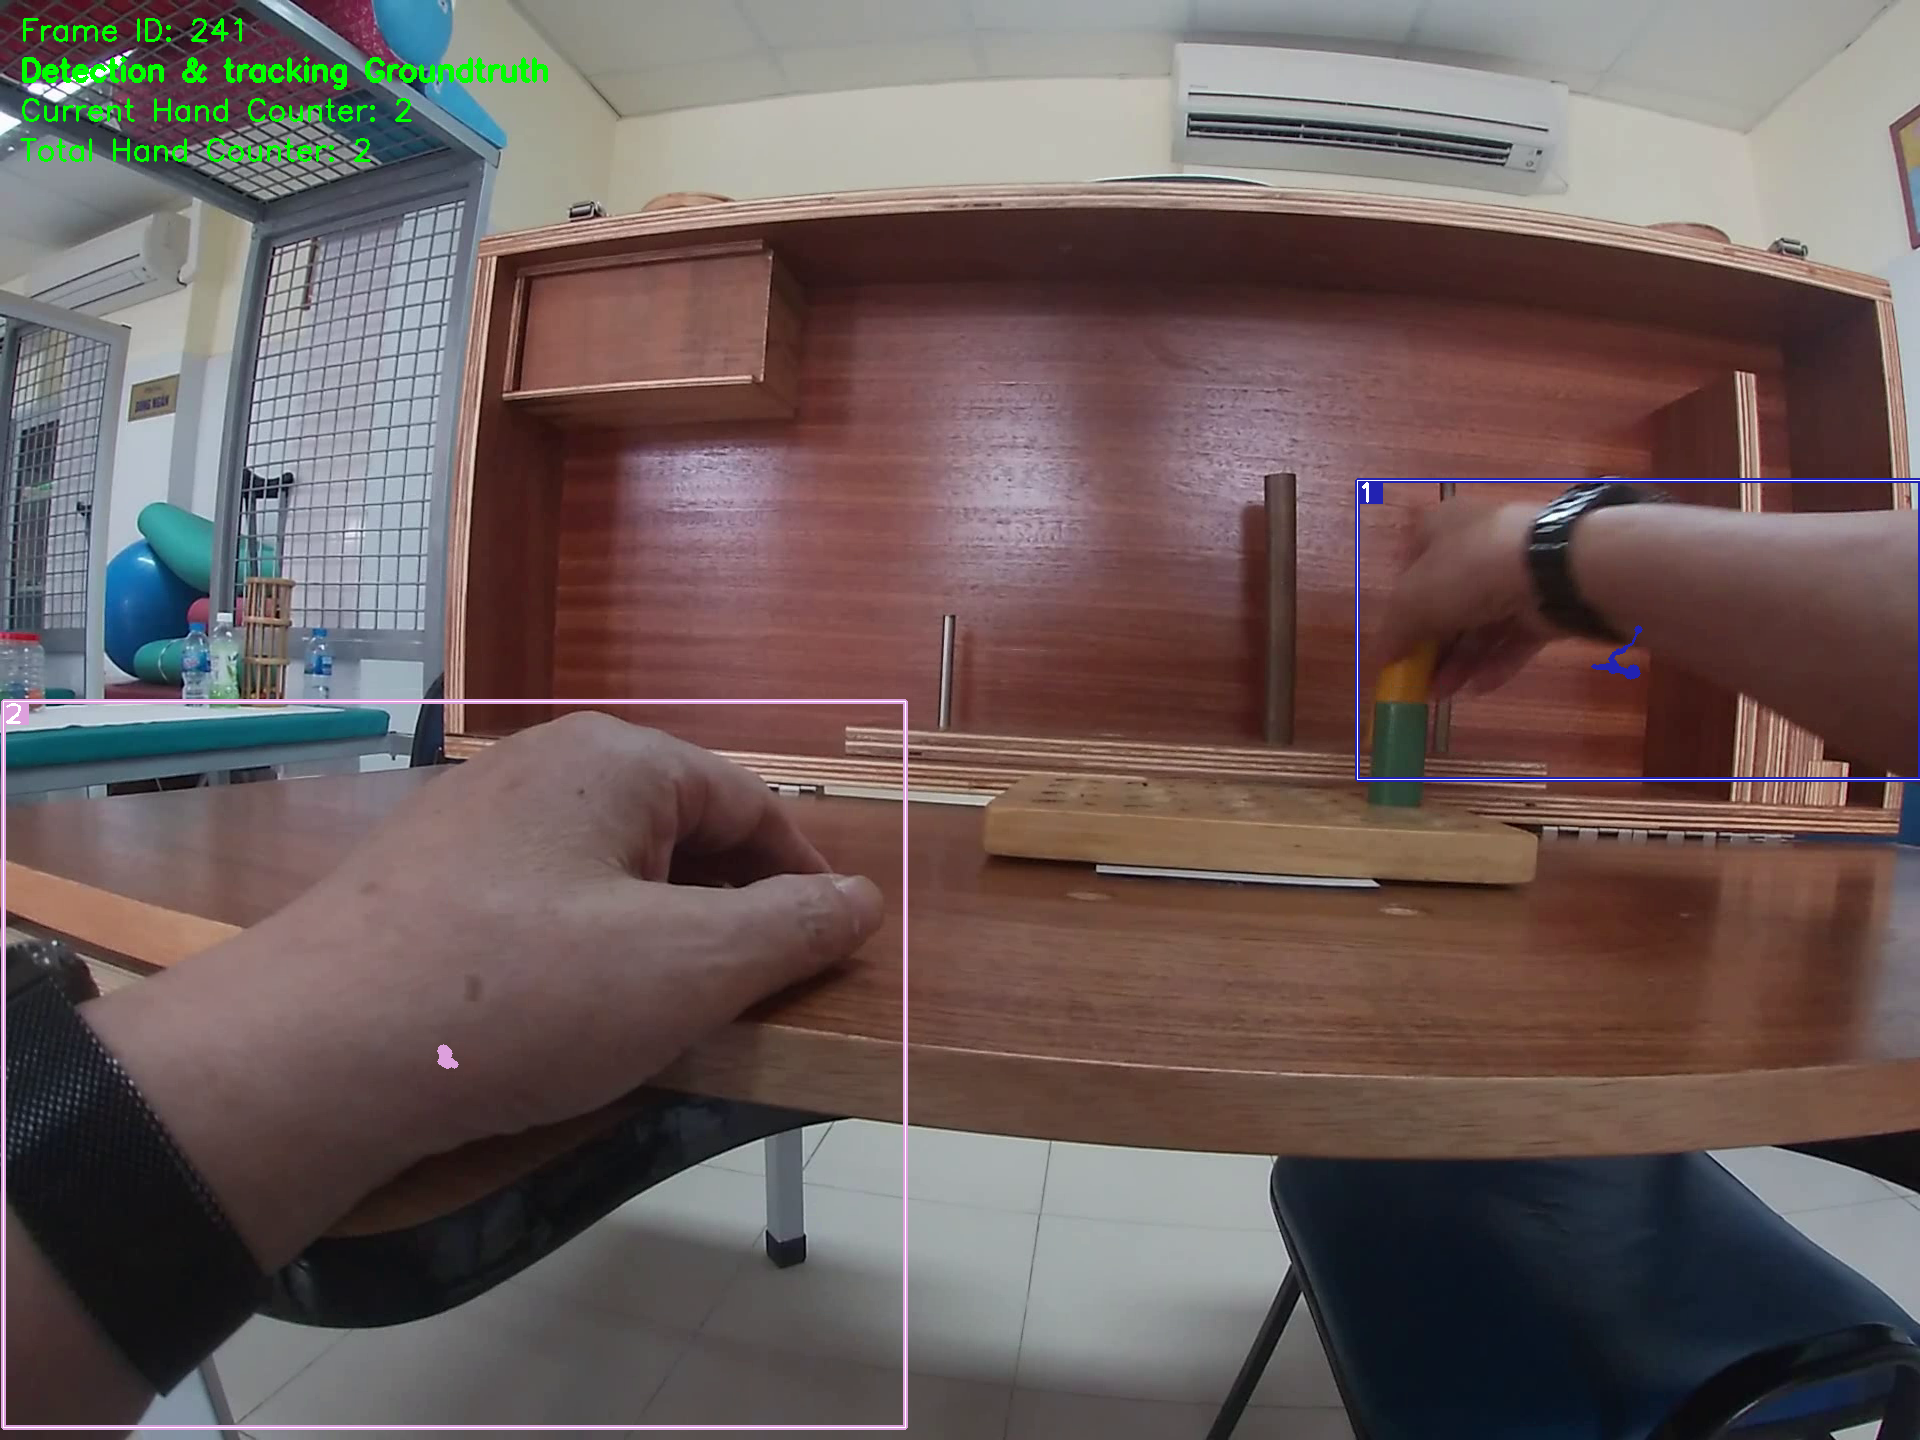
\includegraphics[width=.12\textwidth]{Figs/trajectory/241.png}\hfill
	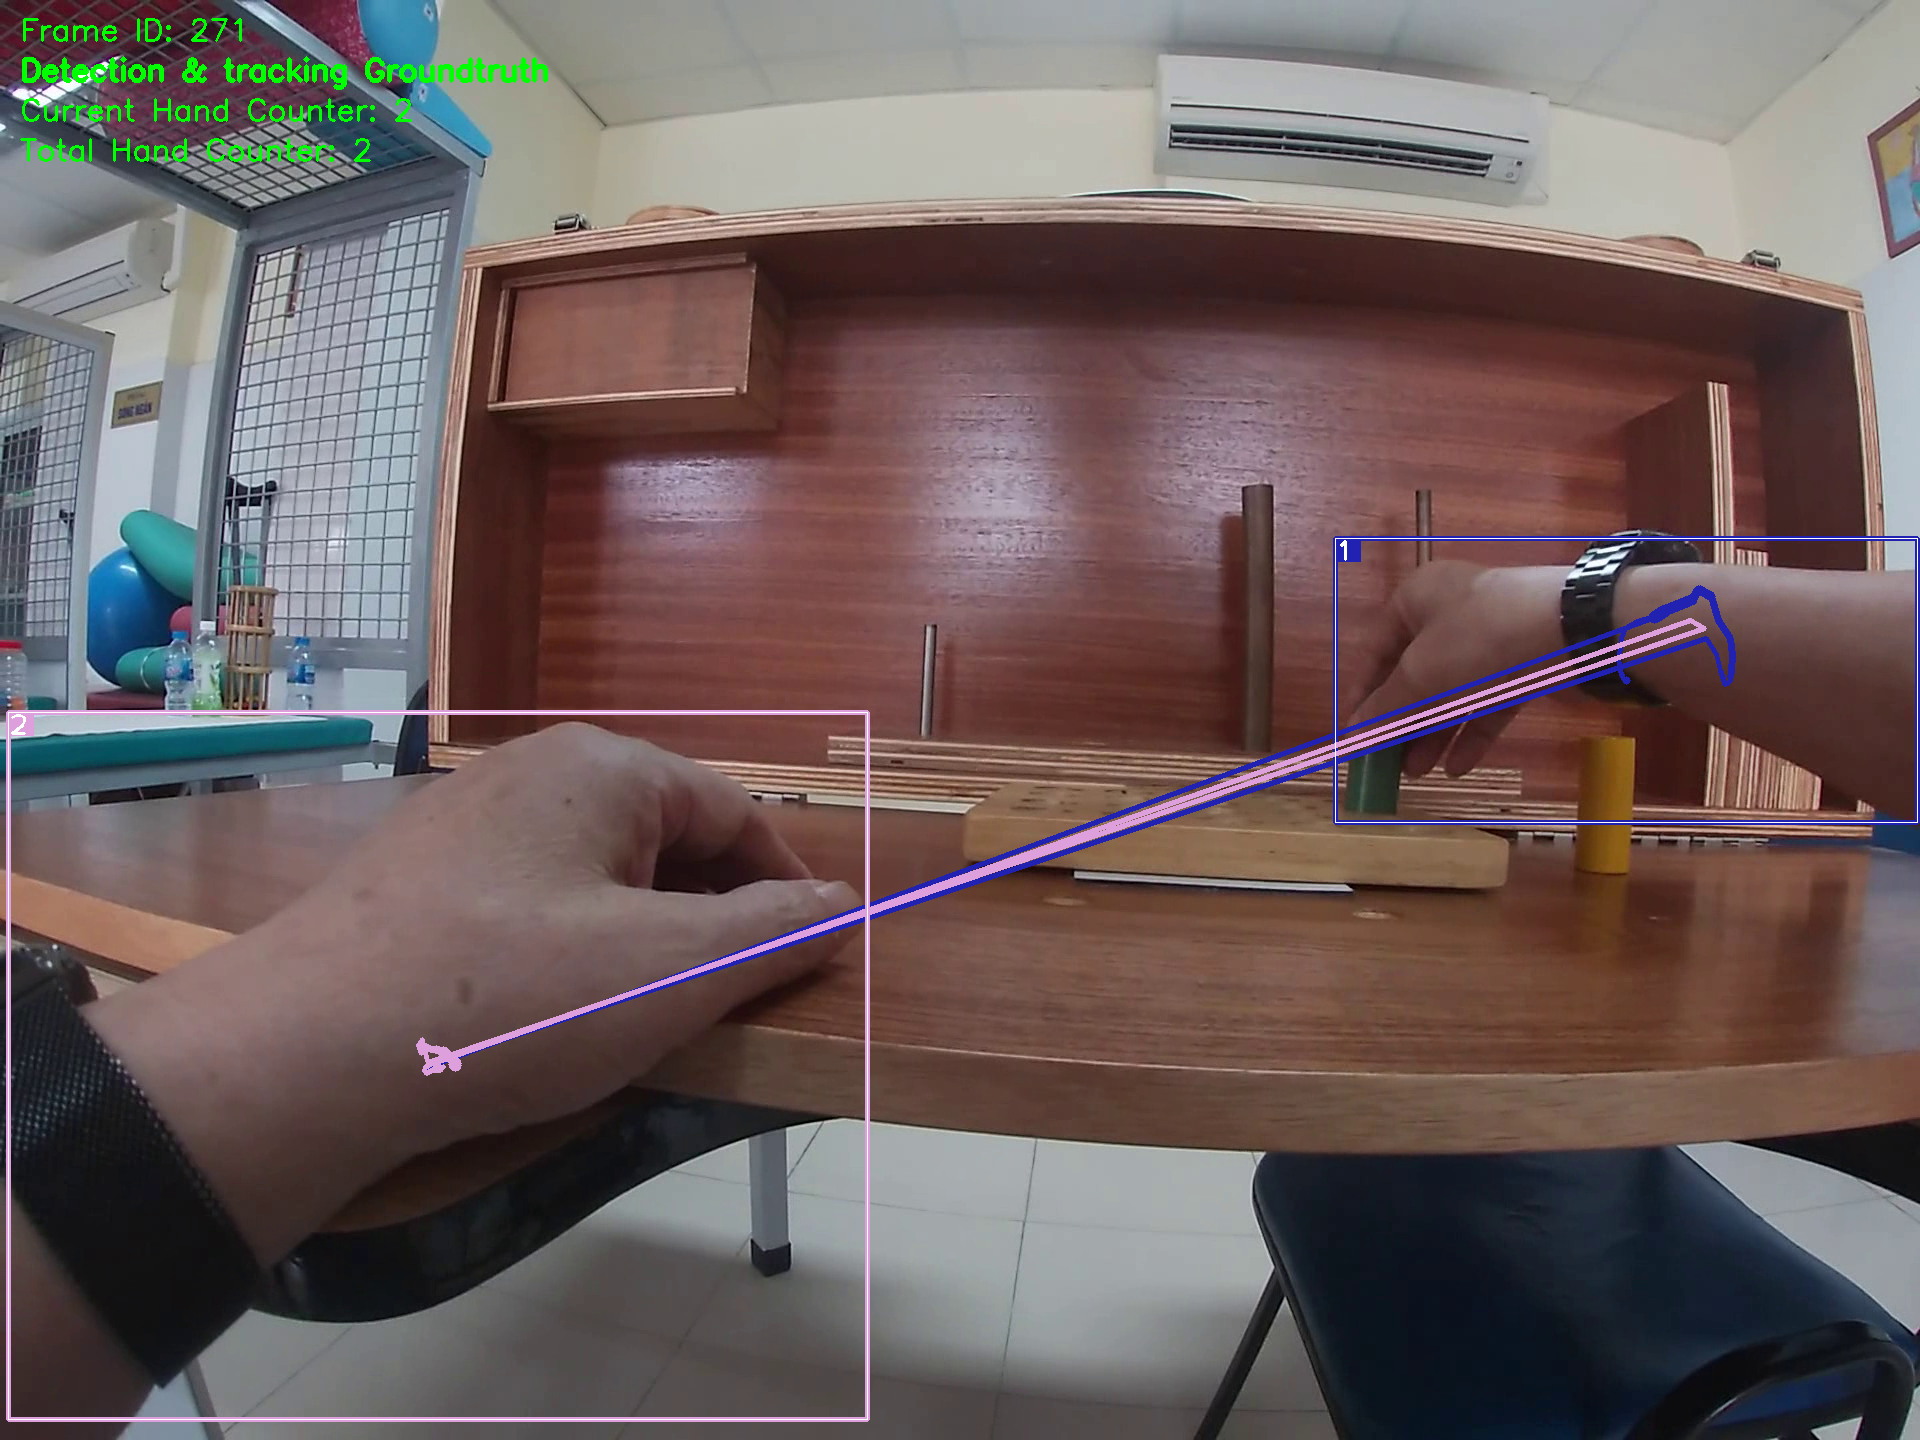
\includegraphics[width=.12\textwidth]{Figs/trajectory/271.png}\hfill	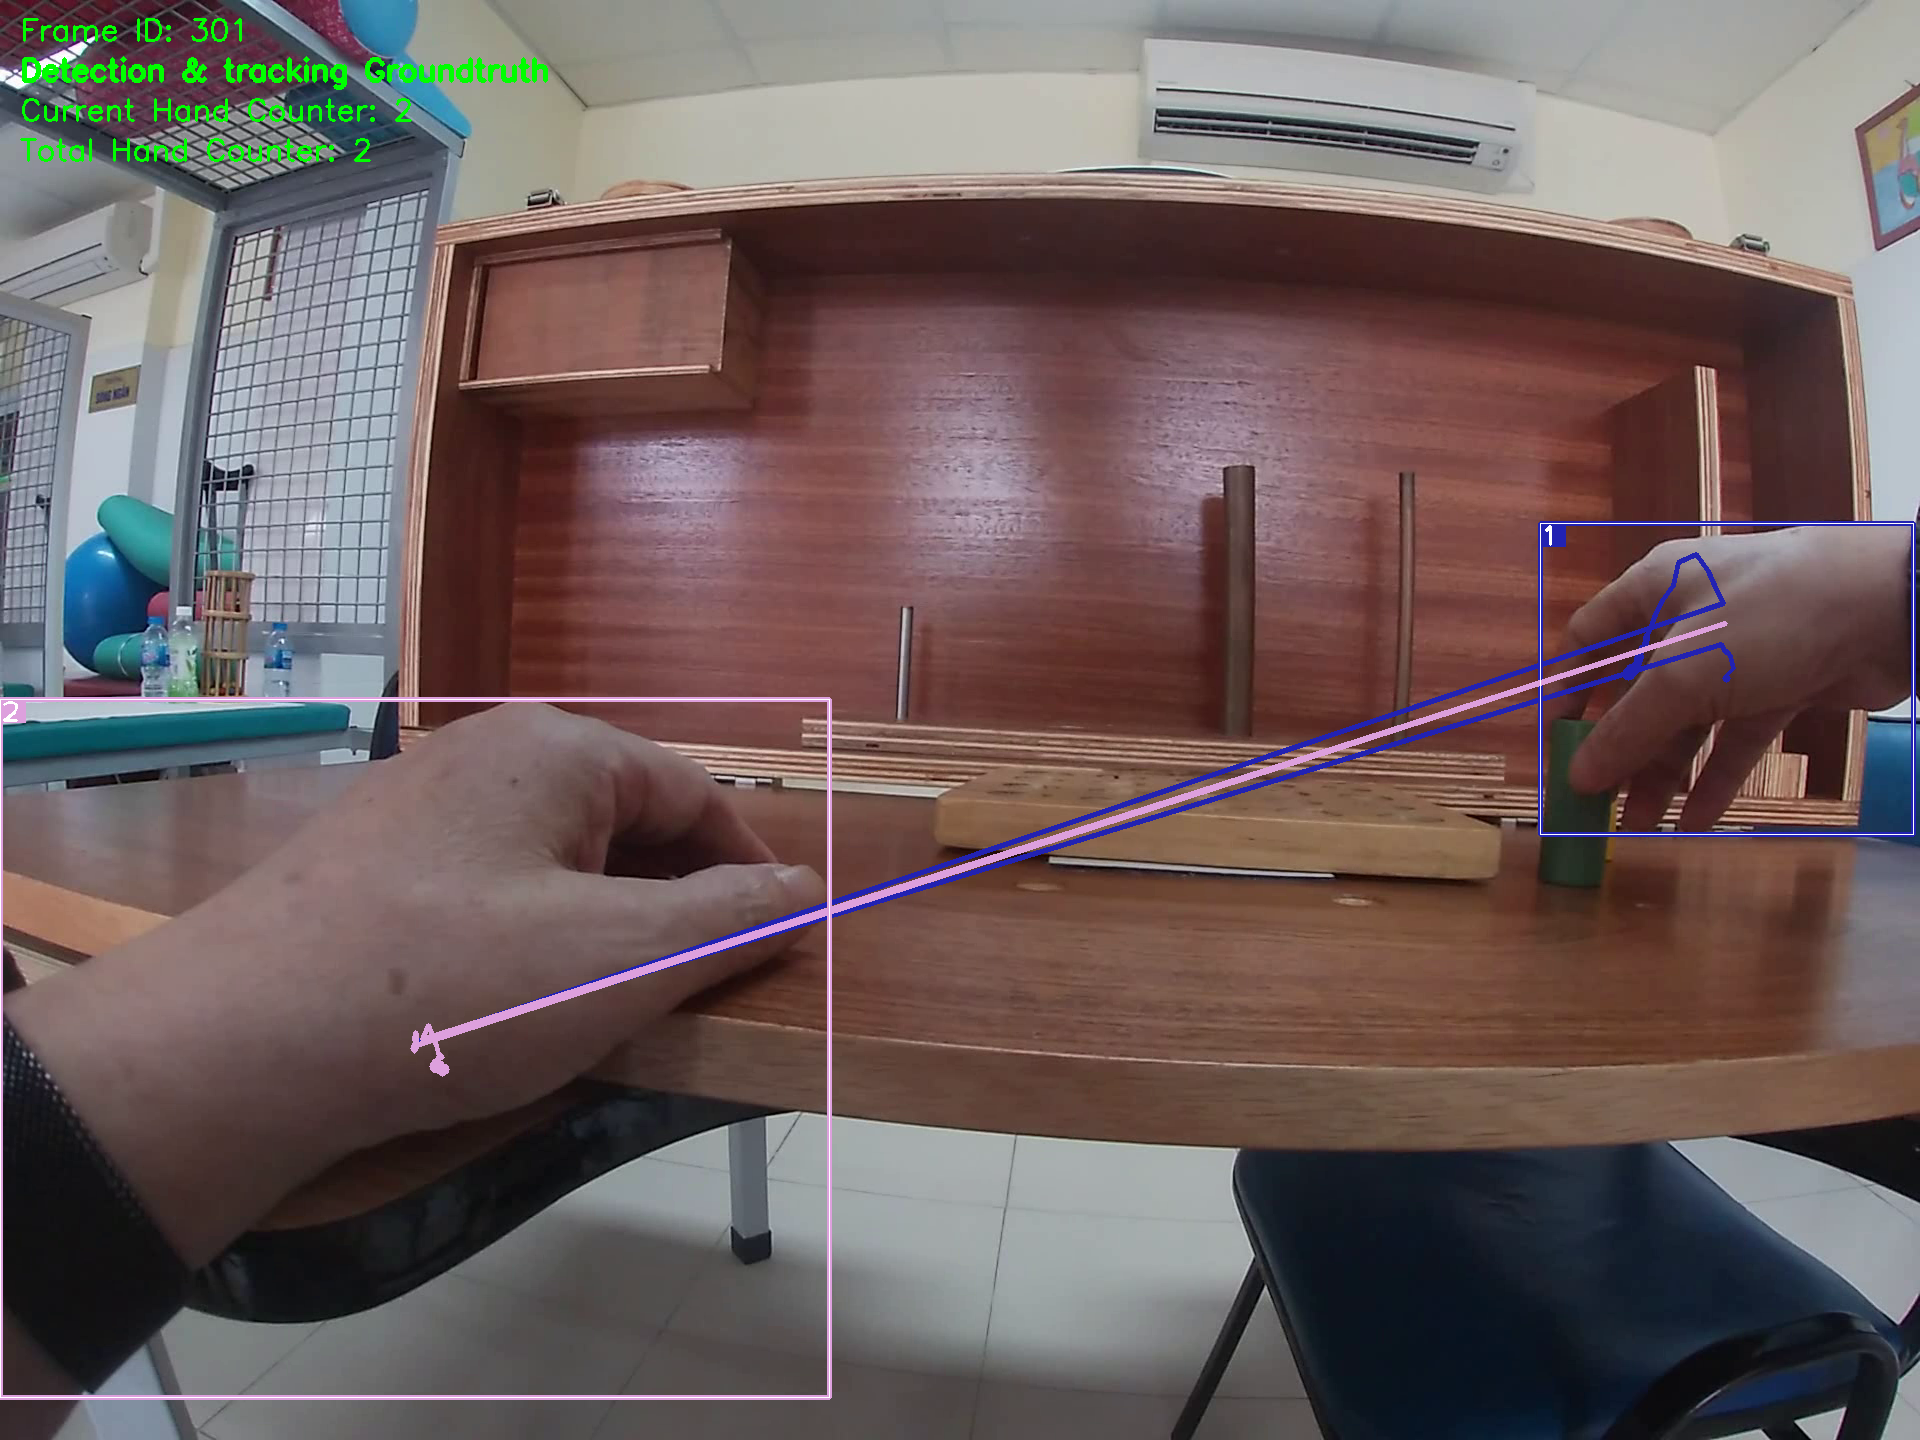
\includegraphics[width=.12\textwidth]{Figs/trajectory/301.png}\hfill
	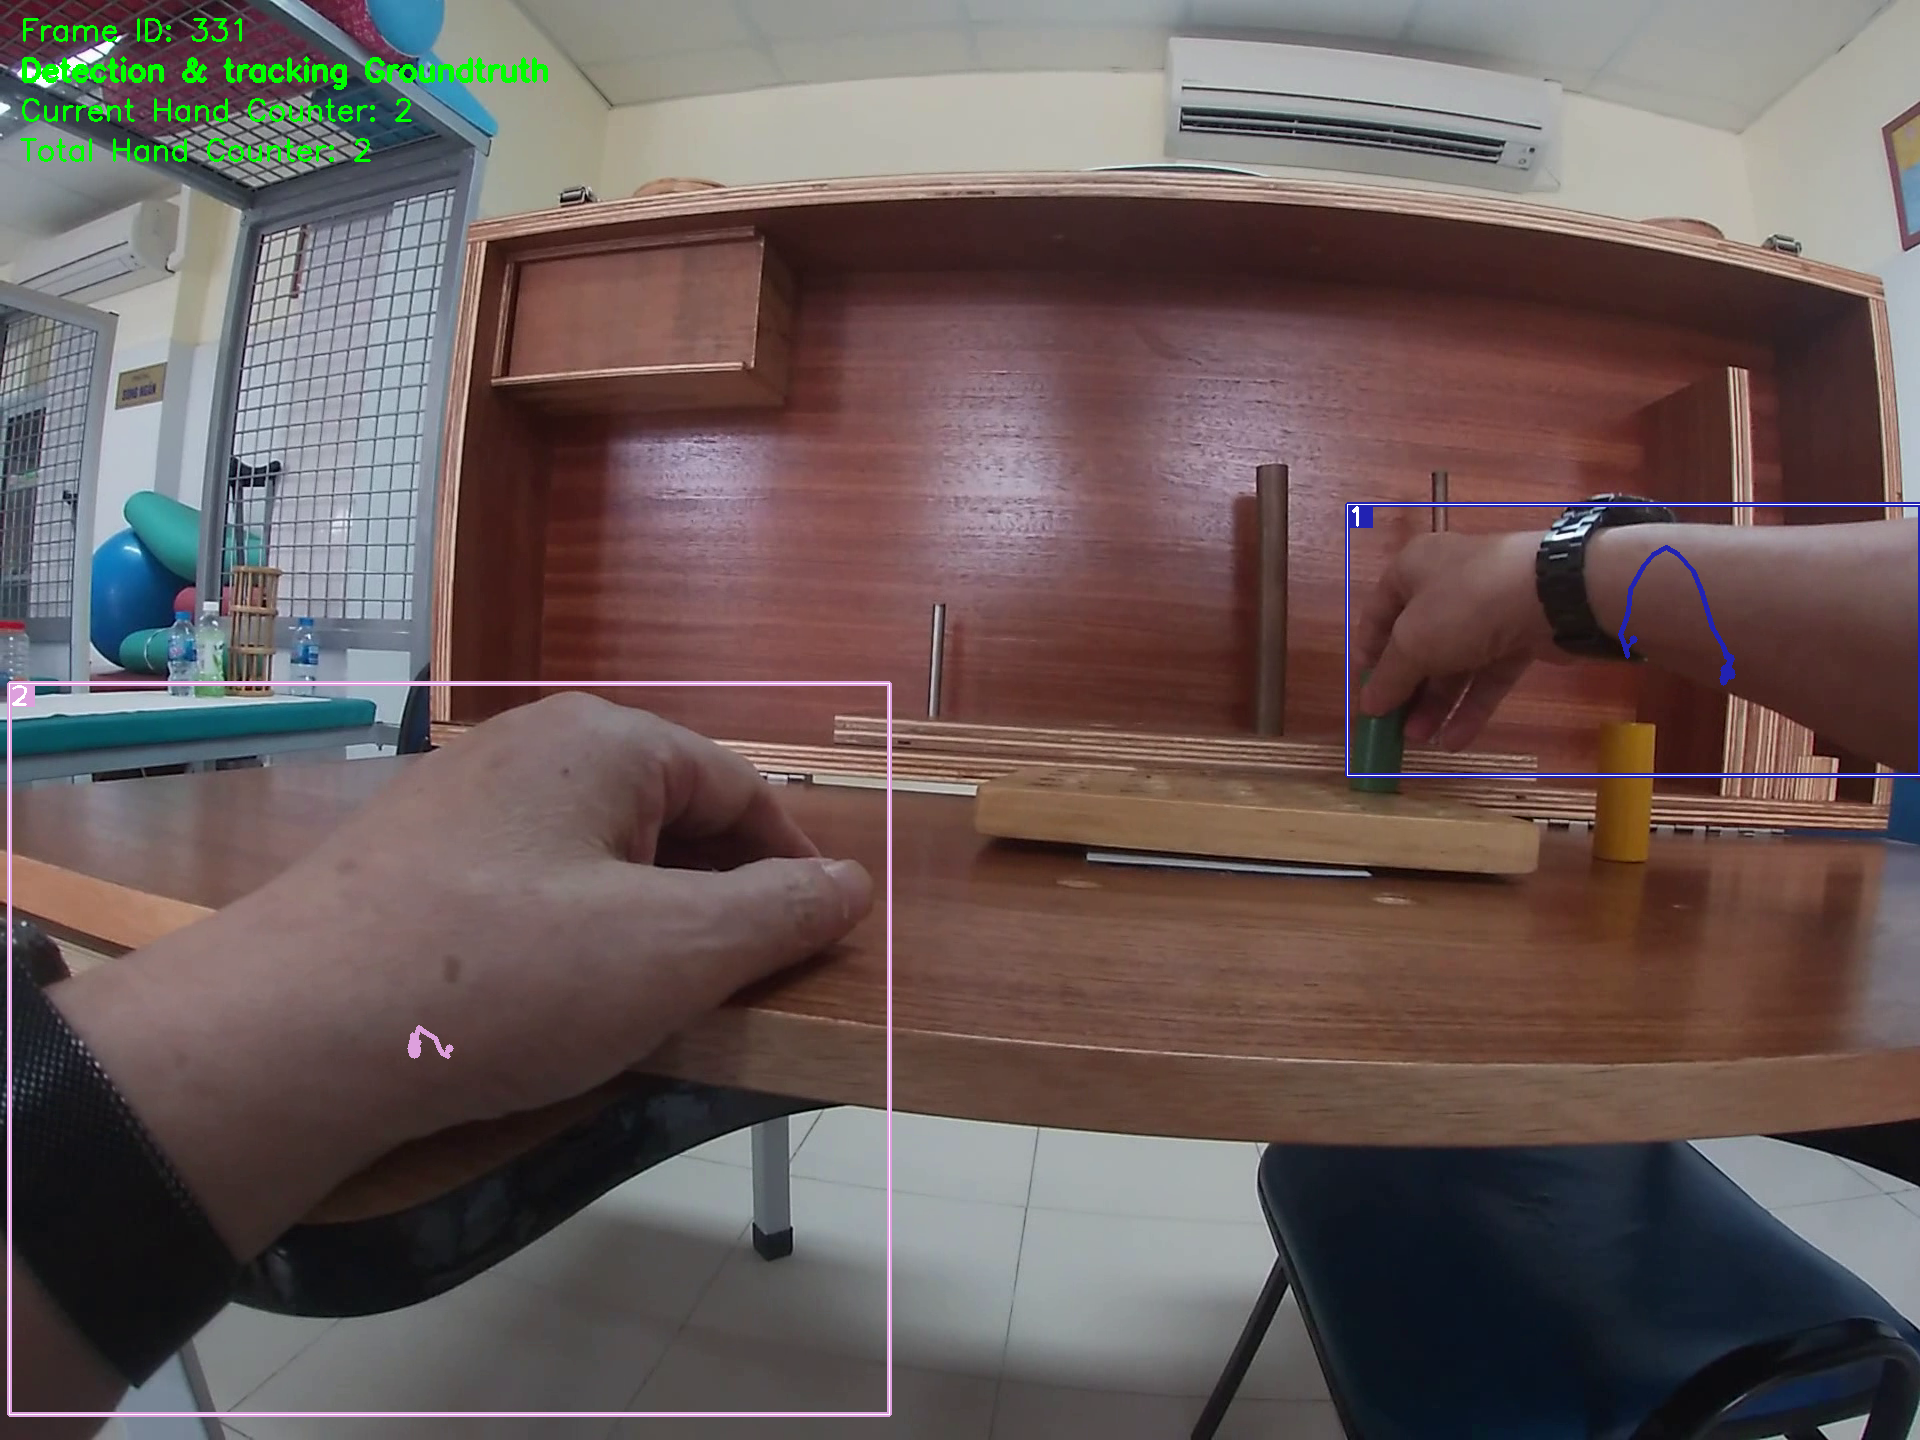
\includegraphics[width=.12\textwidth]{Figs/trajectory/331.png}\hfill
	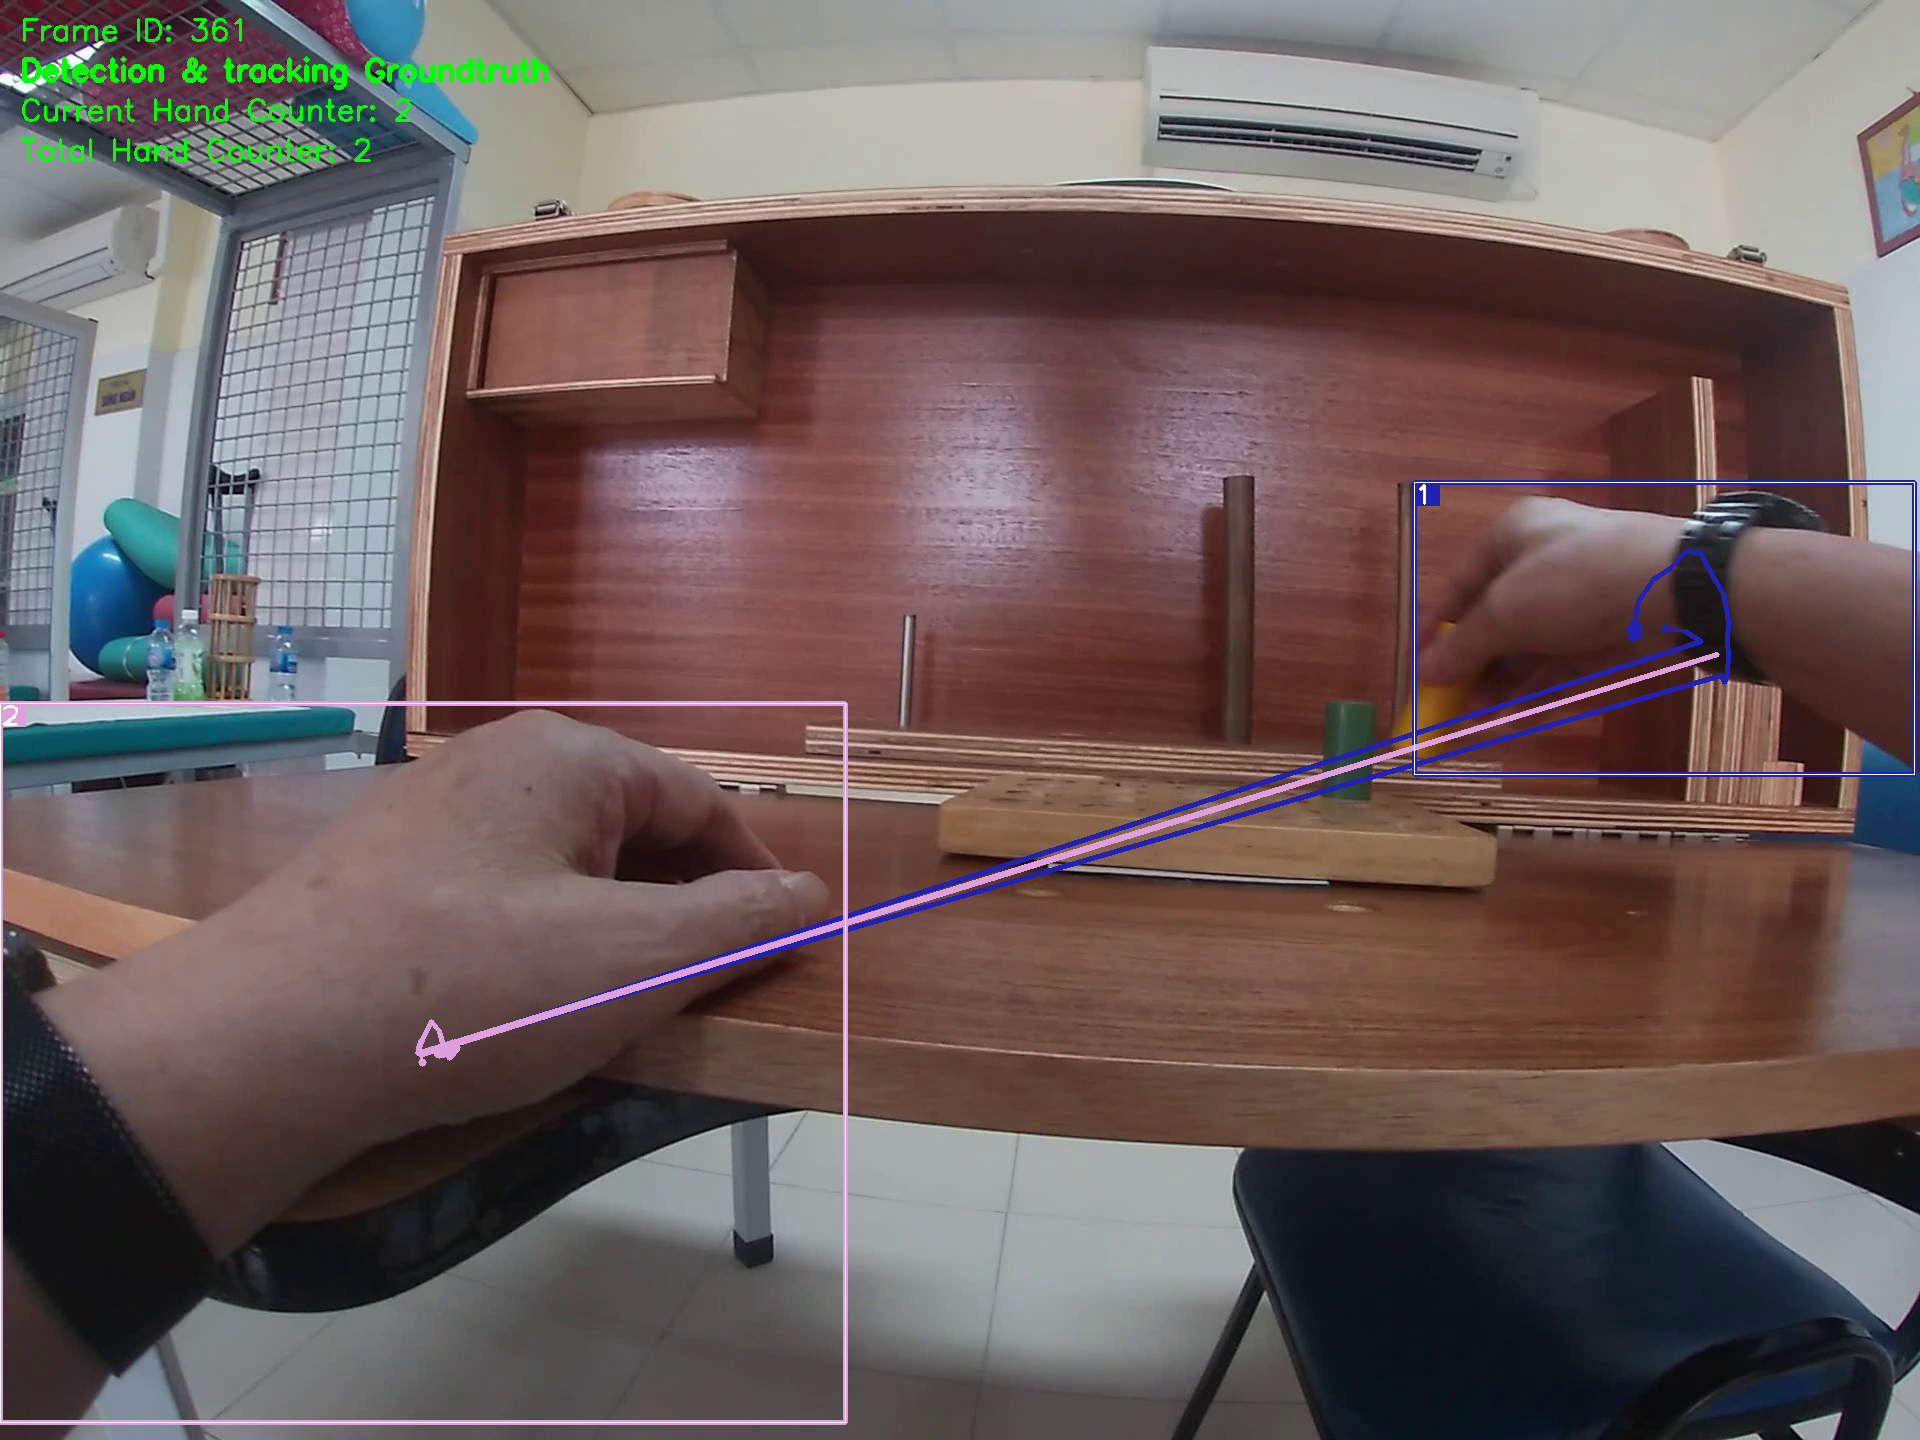
\includegraphics[width=.12\textwidth]{Figs/trajectory/361.png}\hfill
	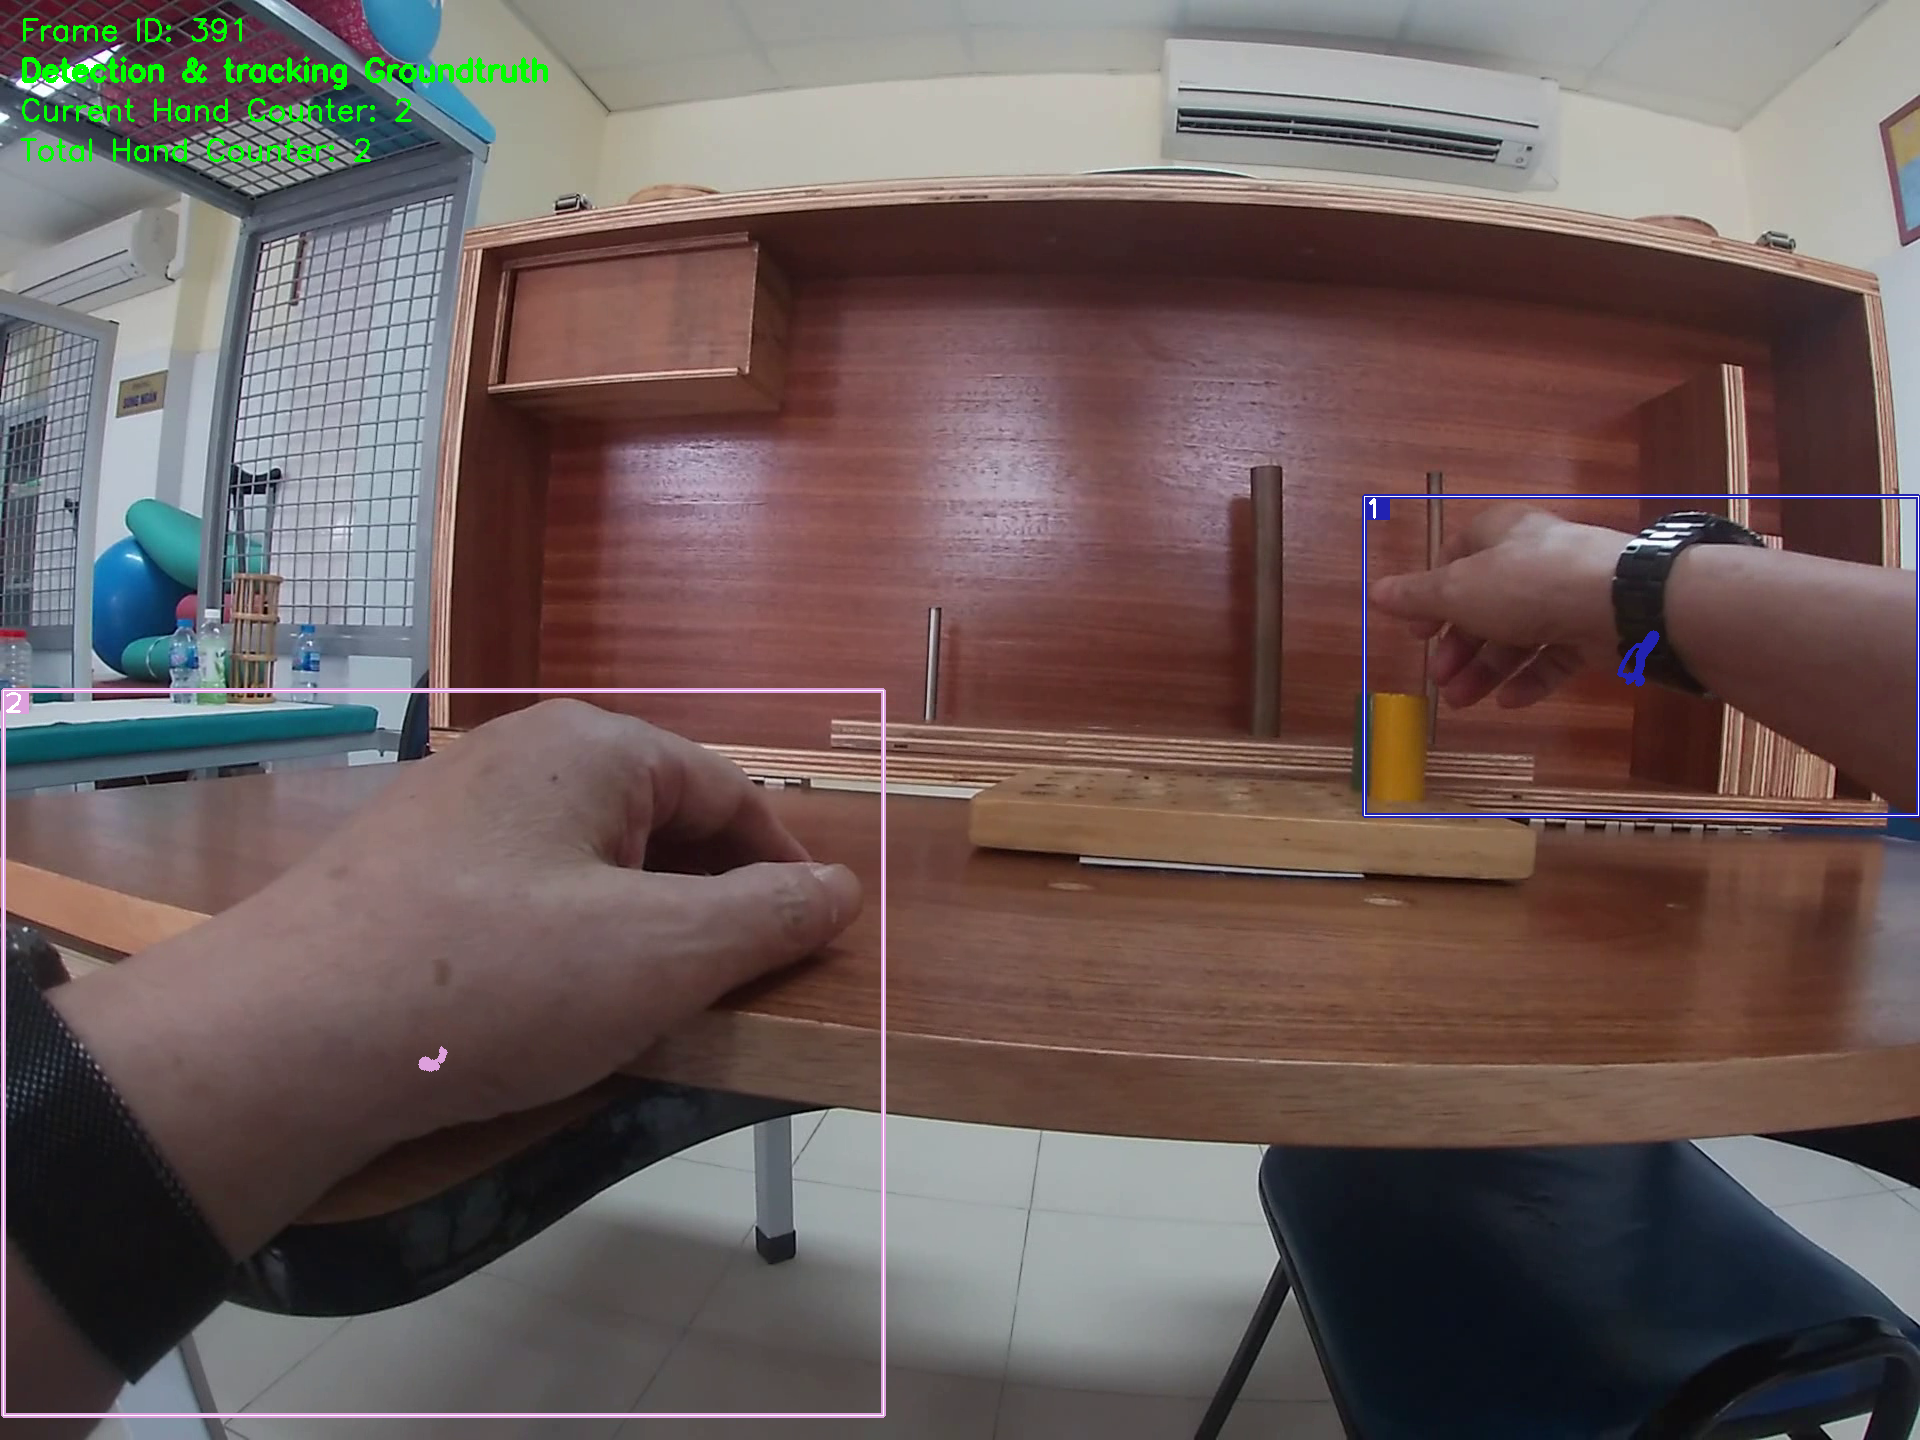
\includegraphics[width=.12\textwidth]{Figs/trajectory/391.png}\hfill	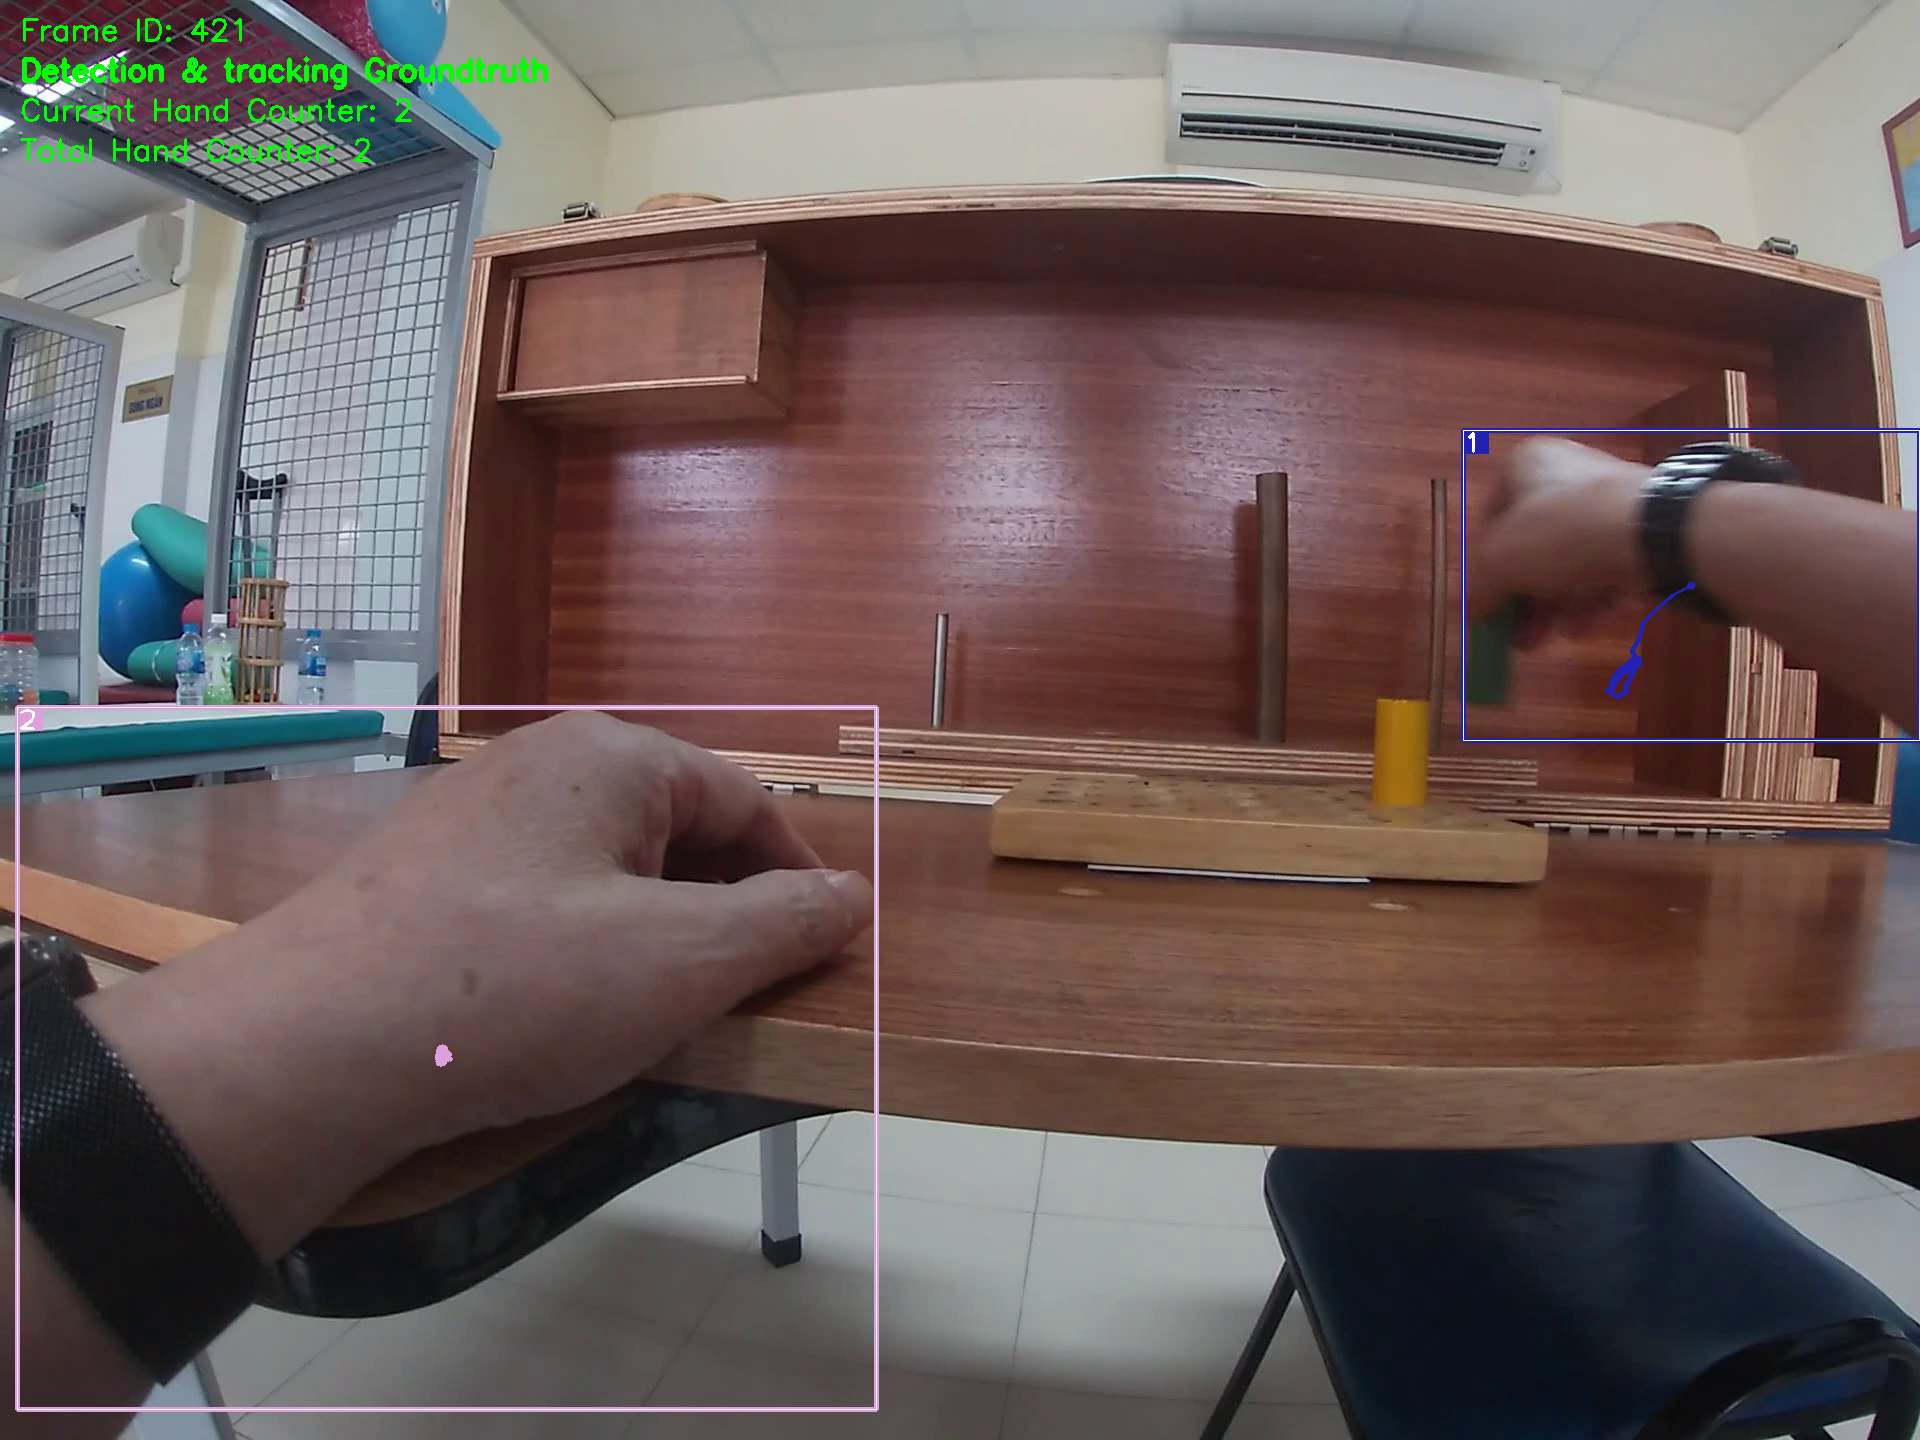
\includegraphics[width=.12\textwidth]{Figs/trajectory/421.png}\hfill
	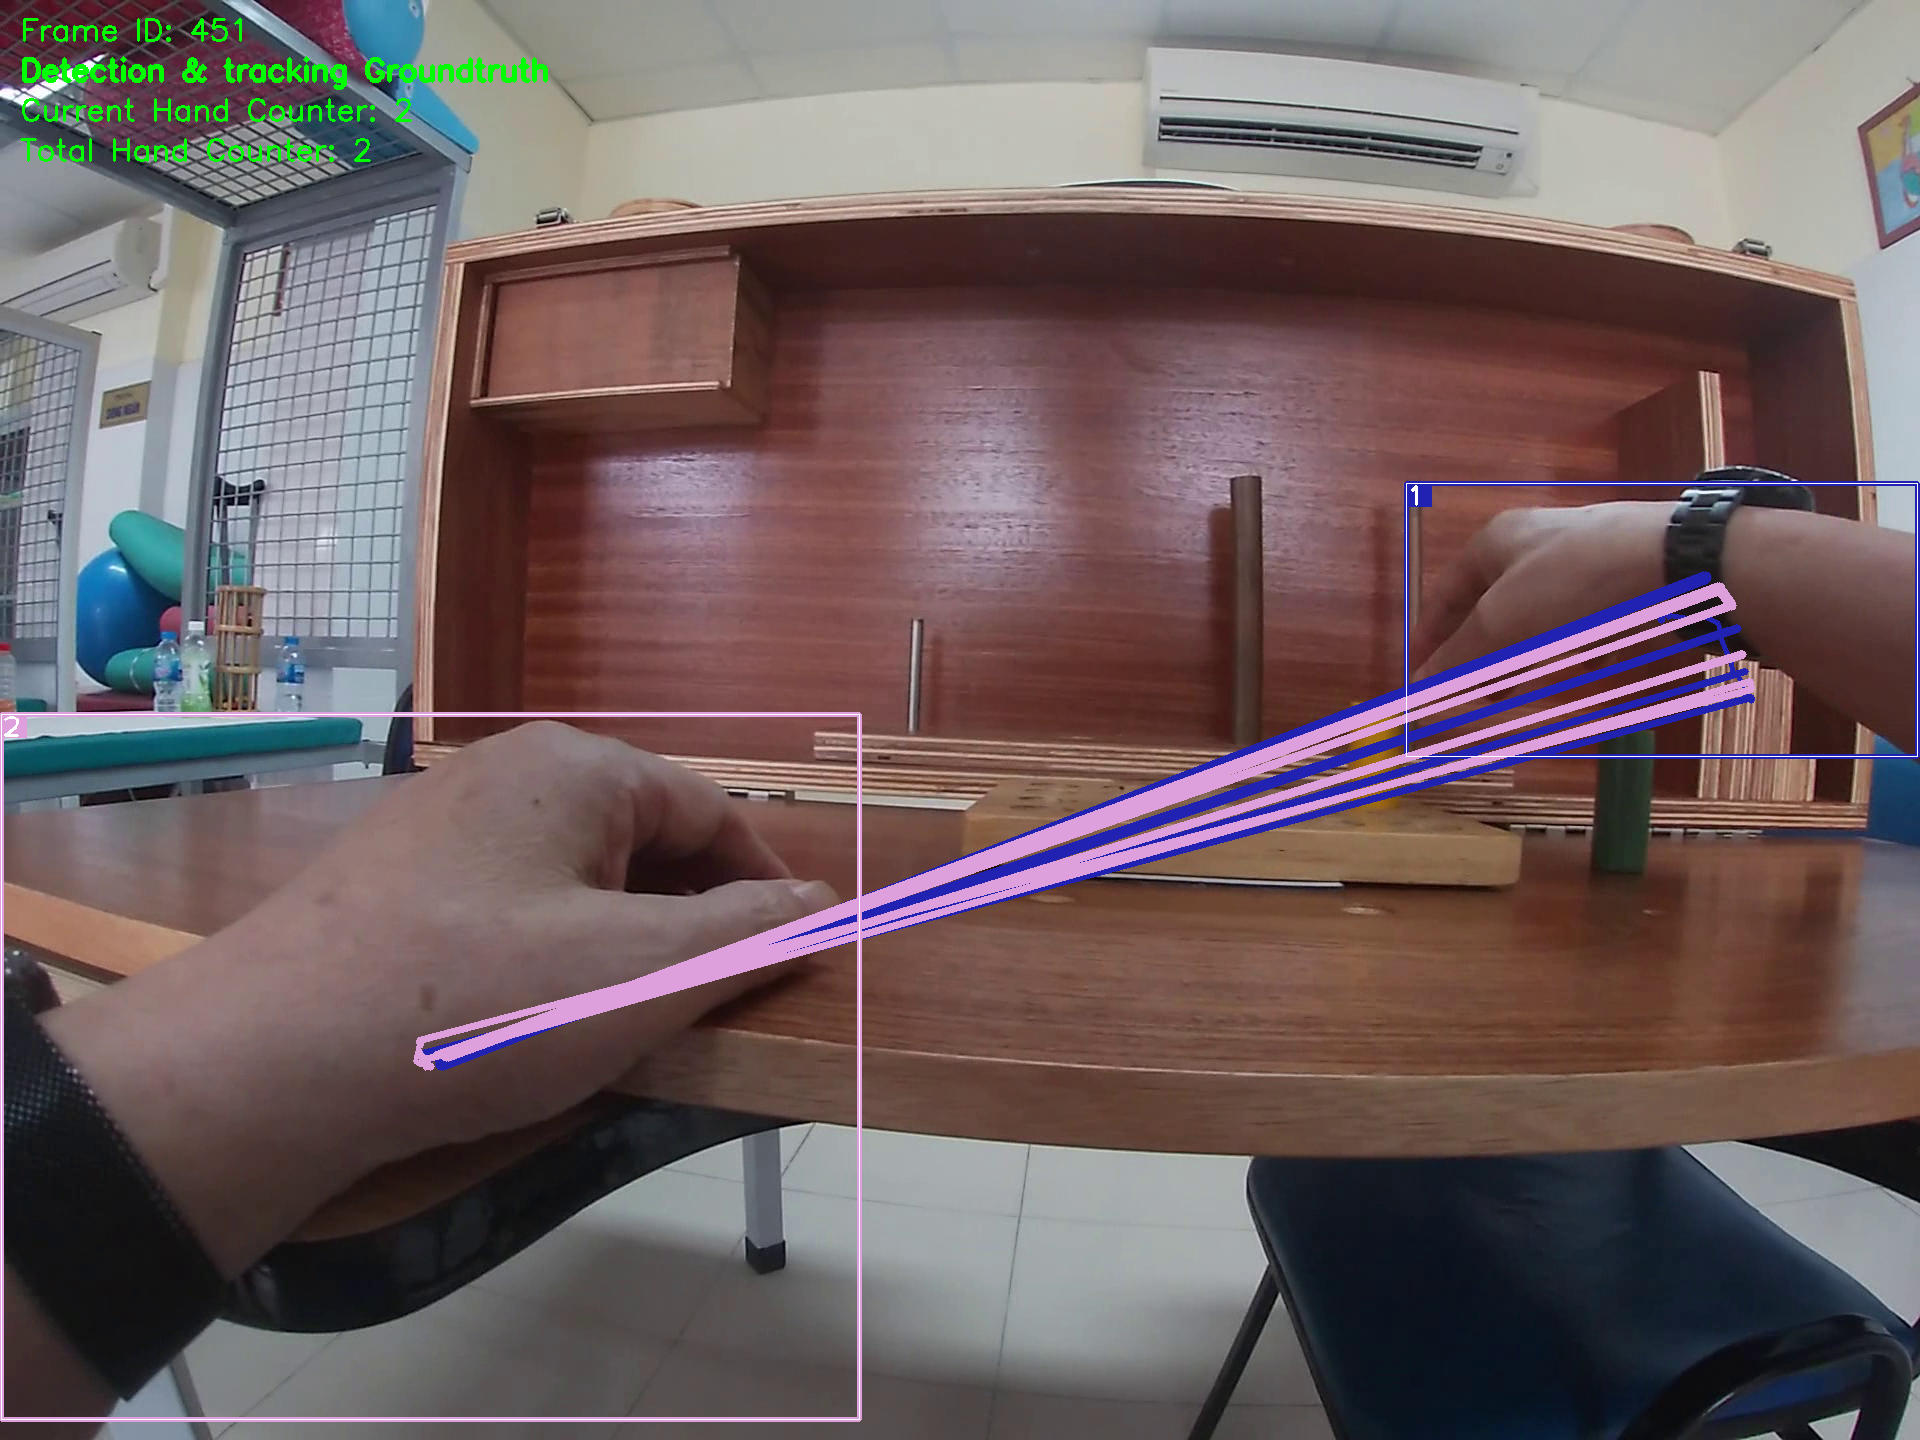
\includegraphics[width=.12\textwidth]{Figs/trajectory/451.png}\hfill
	\caption{Visualization of groundtruth tracklets of patient’s hands practicing with cylinders. Frames extracted from GH010358\_8\_8000\_8547, ordered from left to right, up to down: 1, 31, 61, 91, 121, 151, 181, 211, 241, 271, 301, 311, 361, 391, 421, 451.}
	\label{fig:micand32Trajectory}
\end{figure*}
\begin{figure*}[ht!]
	\centering
	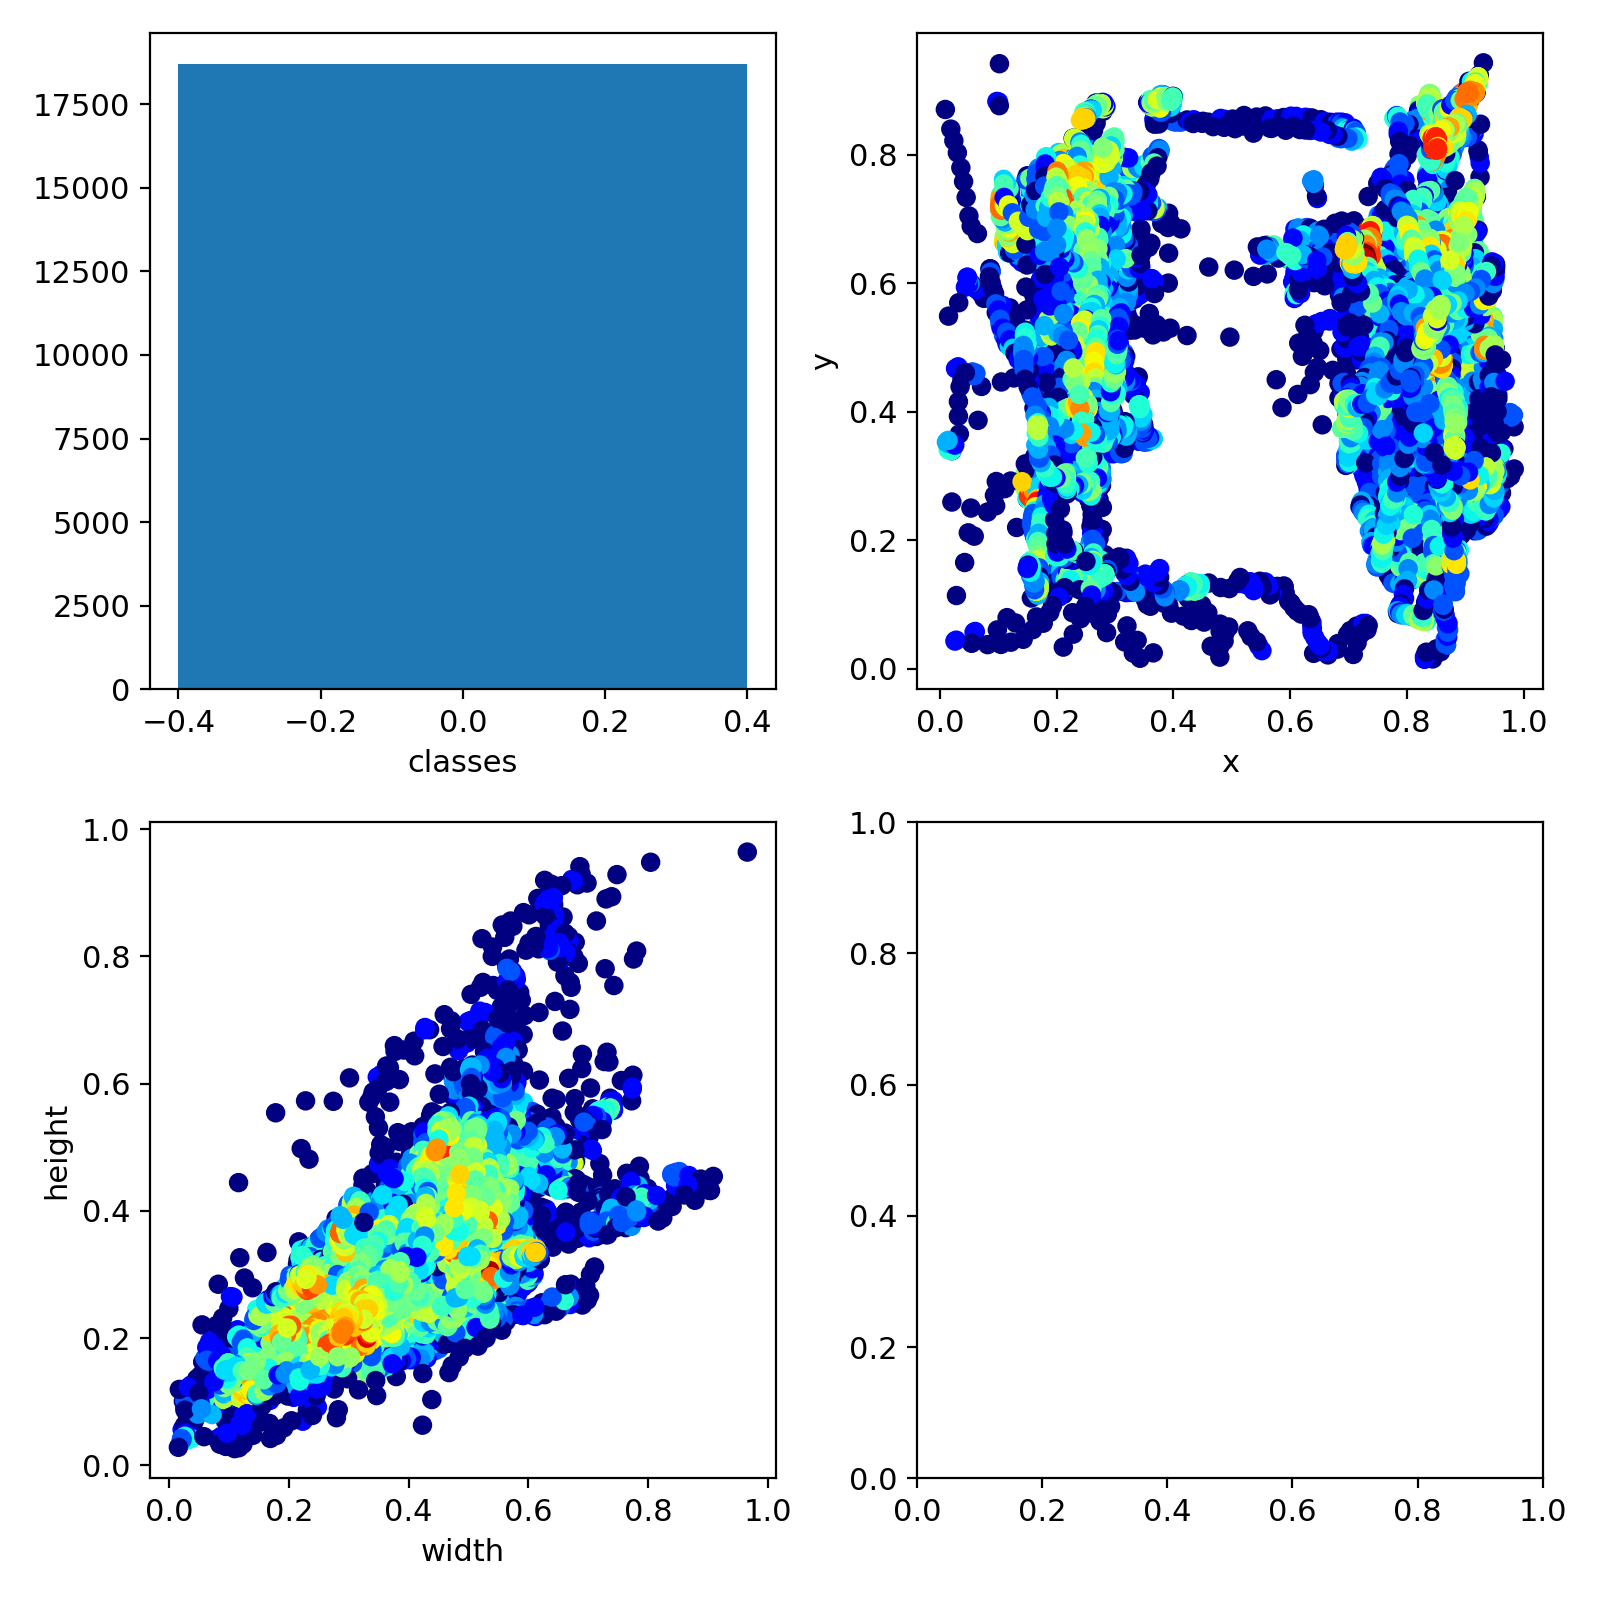
\includegraphics[width=0.48\textwidth]{Figs/yolov5/labels.png}
	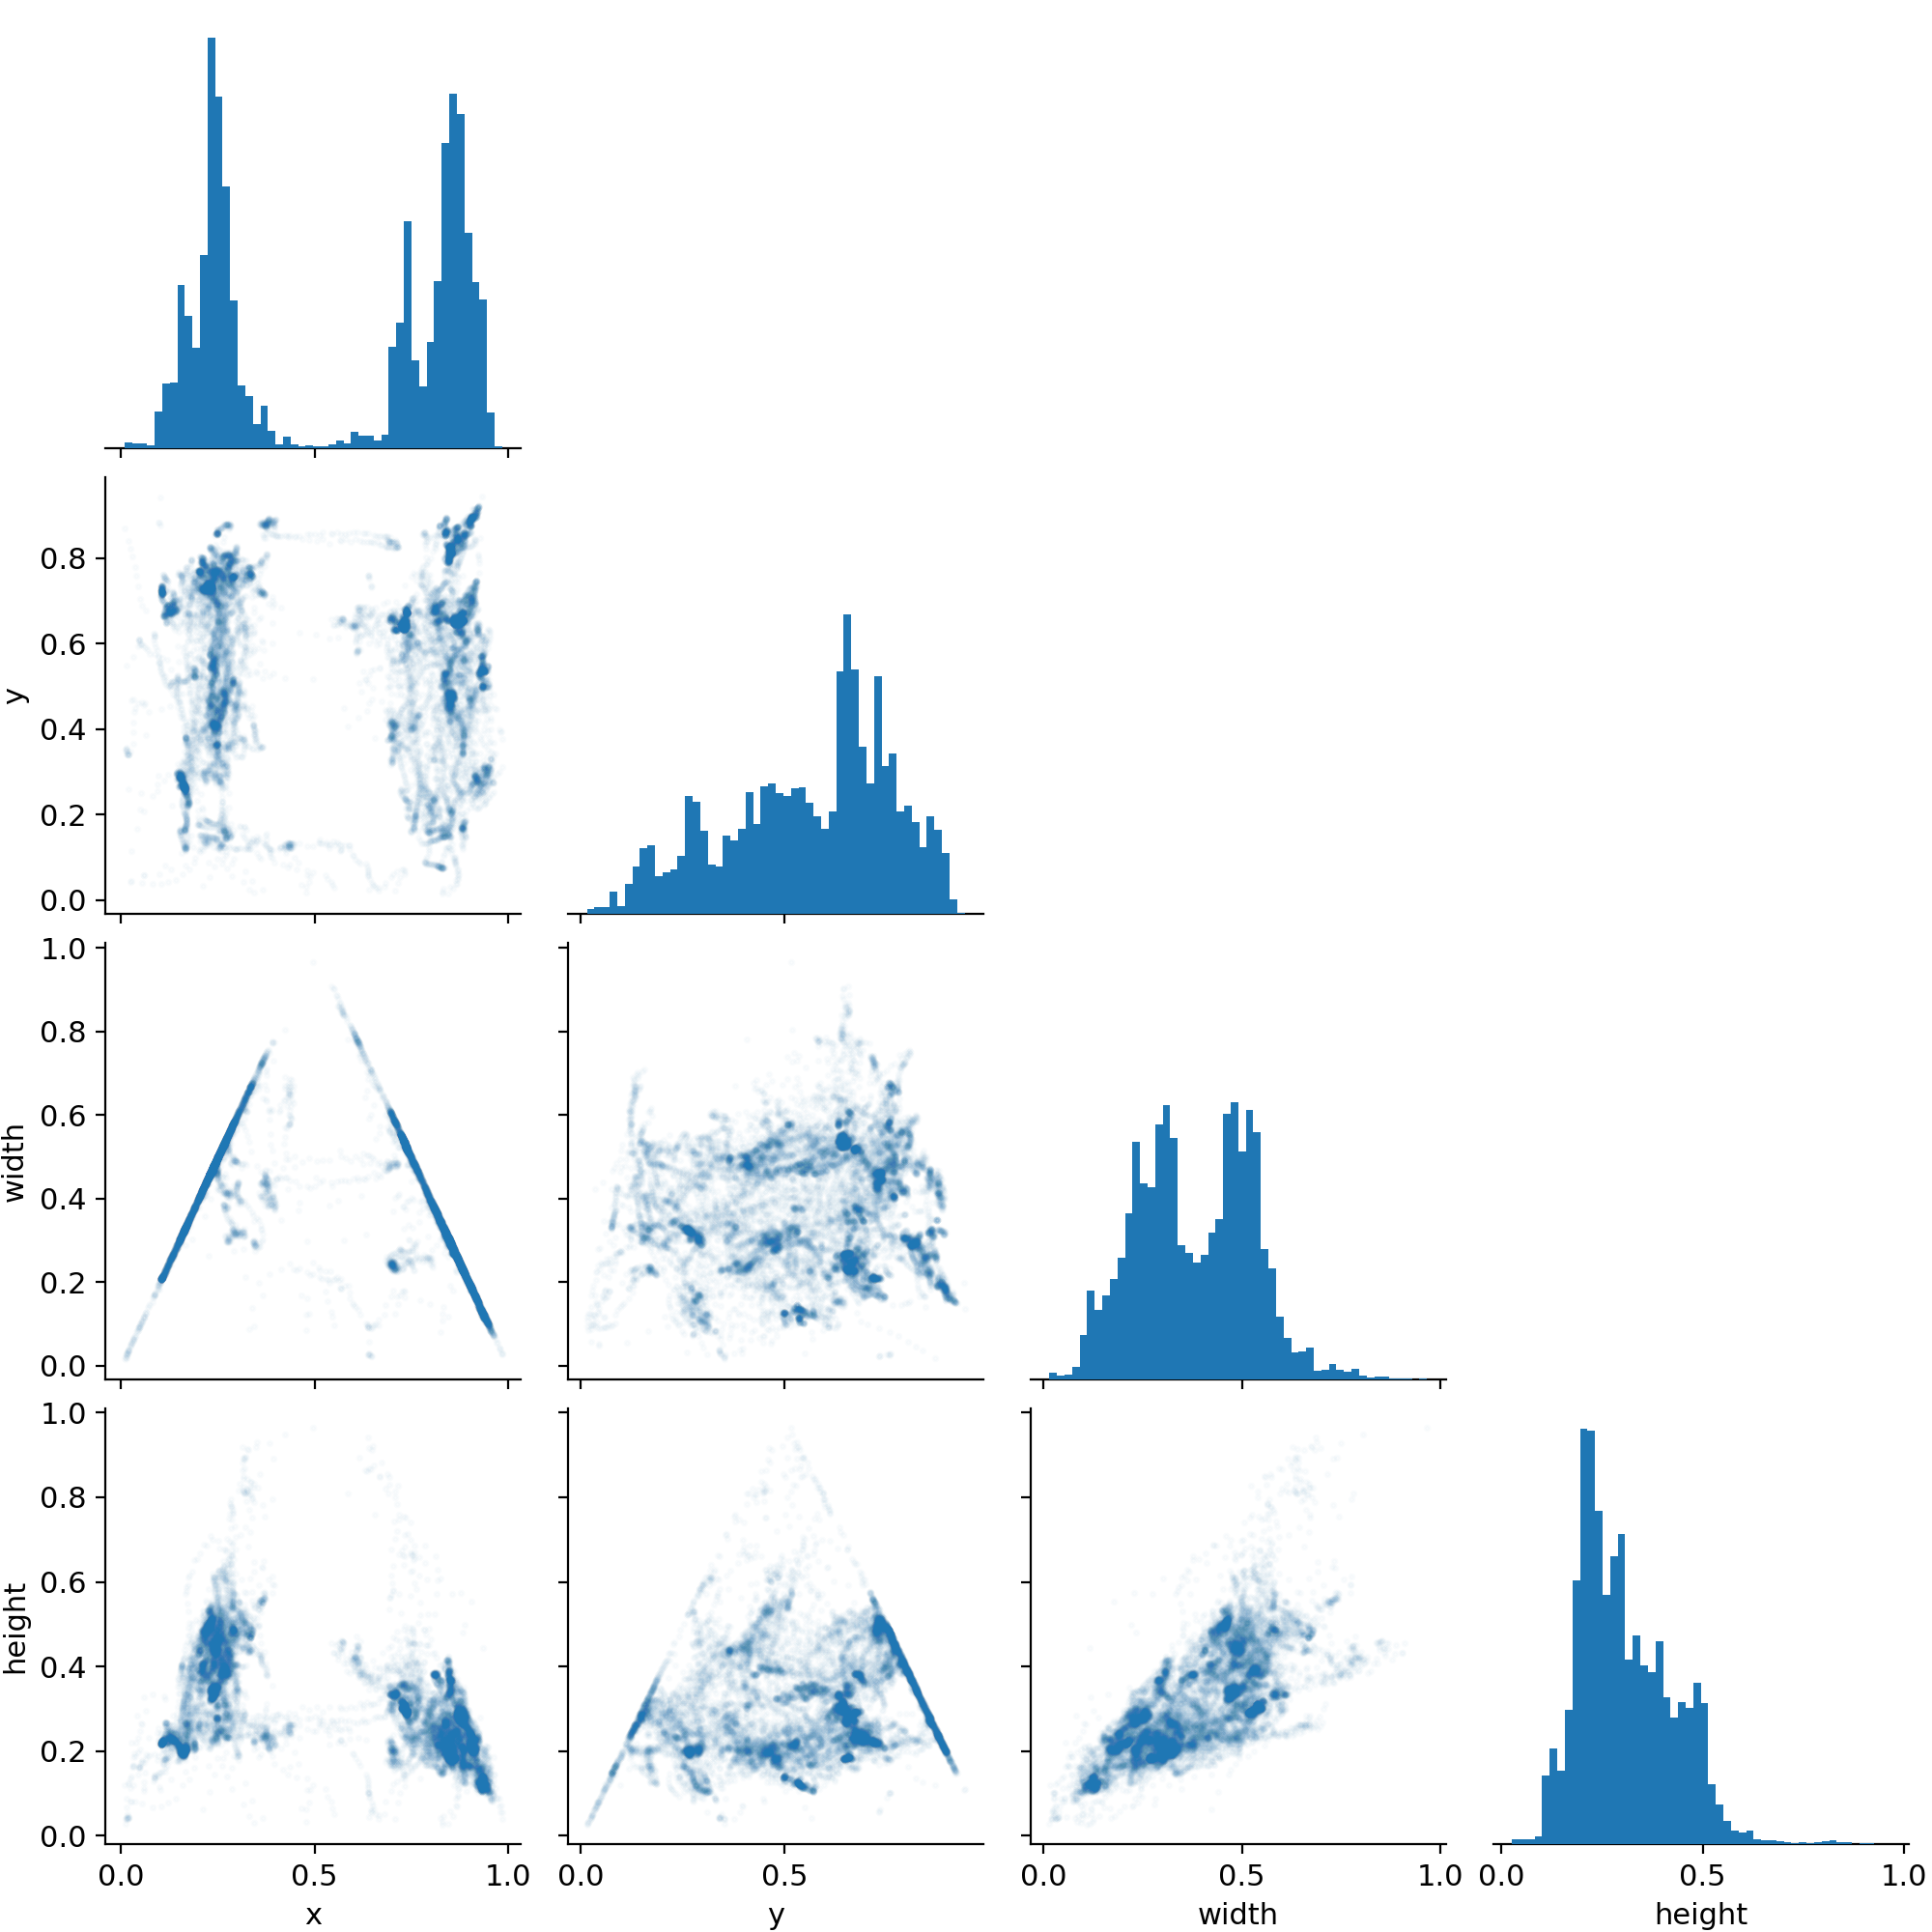
\includegraphics[width=0.48\textwidth]{Figs/yolov5/labels_correlogram.png}
	\caption{Micand32 dataset. Left: labels statistical visualization. Right: labels correlogram.}
	\label{fig:micand32_visualization}
\end{figure*}
Figure \ref{fig:EHTA} shows the working flowchart of EHTA. Initially, annotator selected 1 model from model zoo that was pre-trained on COCO, GTEA family and EgoHands datasets, for example, this thesis used FasterRCNNR50FPN3x. Input is a set of frames in 1 sequence. For each frame, reference the model on the frame to predict the position of the hands and get the detection of bounding box and confidence score. Next, use the VIA tool to display the prediction in frames, observe and make comments to write code. From observation and experience with the dataset, writing code to automatically editing the labels for the hand’s position and identification. Then shows the automatically assigned label portion. If the label is not correct, manually correct the bounding box position, add or remove the bounding box, or correct the incorrect ID. Finally, save ground-truth according to MOT Challenge standards for training, testing and evaluation in txt format. At the same time, save ground-truth video for debugging.
\begin{figure}
	\centerline{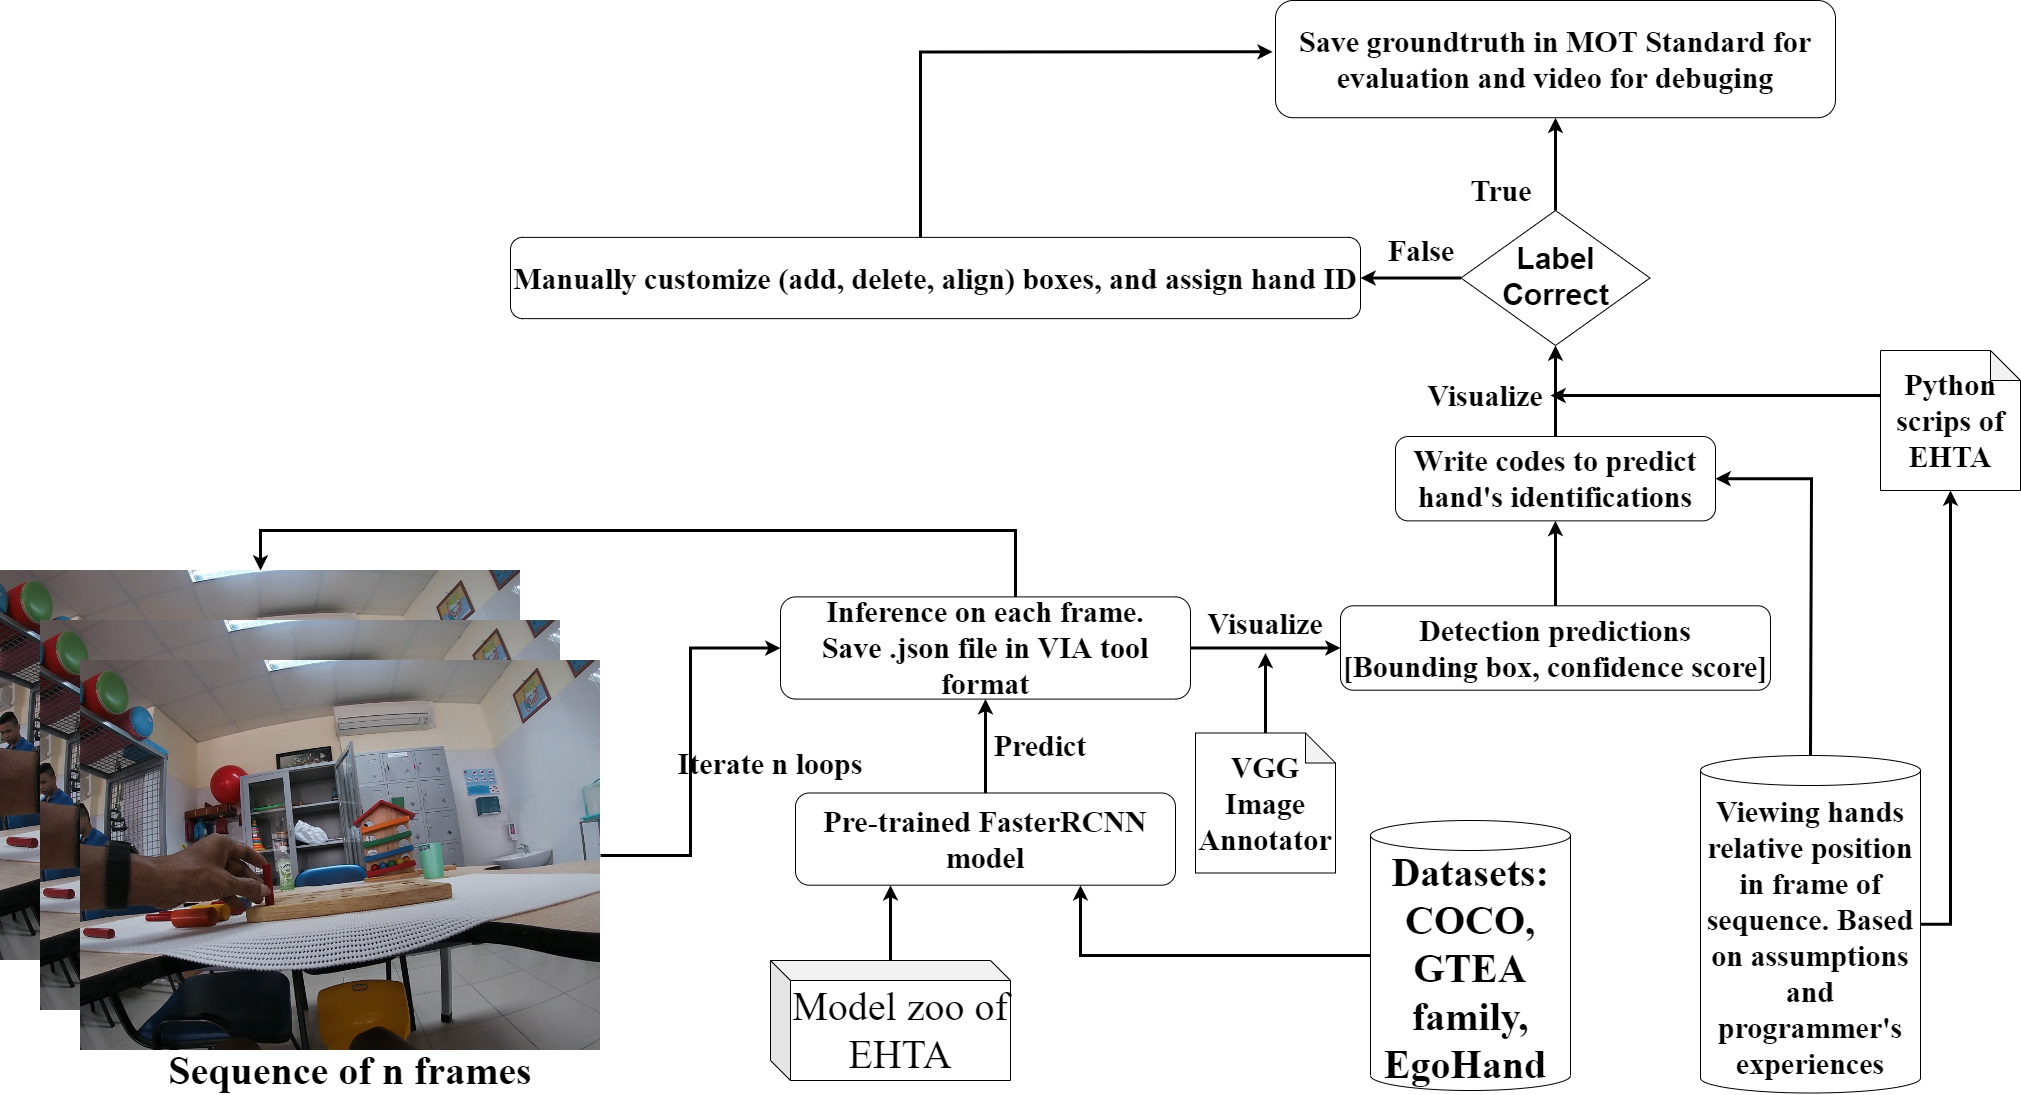
\includegraphics[width=1\linewidth]{Figs/EHTAflowchartPage2.png}}
	\caption{The workflow of EHTA.}
	\label{fig:EHTA}
\end{figure}
Annotation time for 1 image with manually and semi-automatically by EHTA is respectively 5 seconds and 1 second. By using EHTA, the subjectivity of human perception and loss of time are reduced as well as consistency and coordination among different individuals' annotations are accomplished.
%% This is an example first chapter.  You should put chapter/appendix that you
%% write into a separate file, and add a line \include{yourfilename} to
%% main.tex, where `yourfilename.tex' is the name of the chapter/appendix file.
%% You can process specific files by typing their names in at the 
%% \files=
%% prompt when you run the file main.tex through LaTeX.
\chapter{Proposed Framework}\label{chap:framework}

\section{Proposed framework: tracking by detection}
\begin{figure}[htbp]
	\centerline{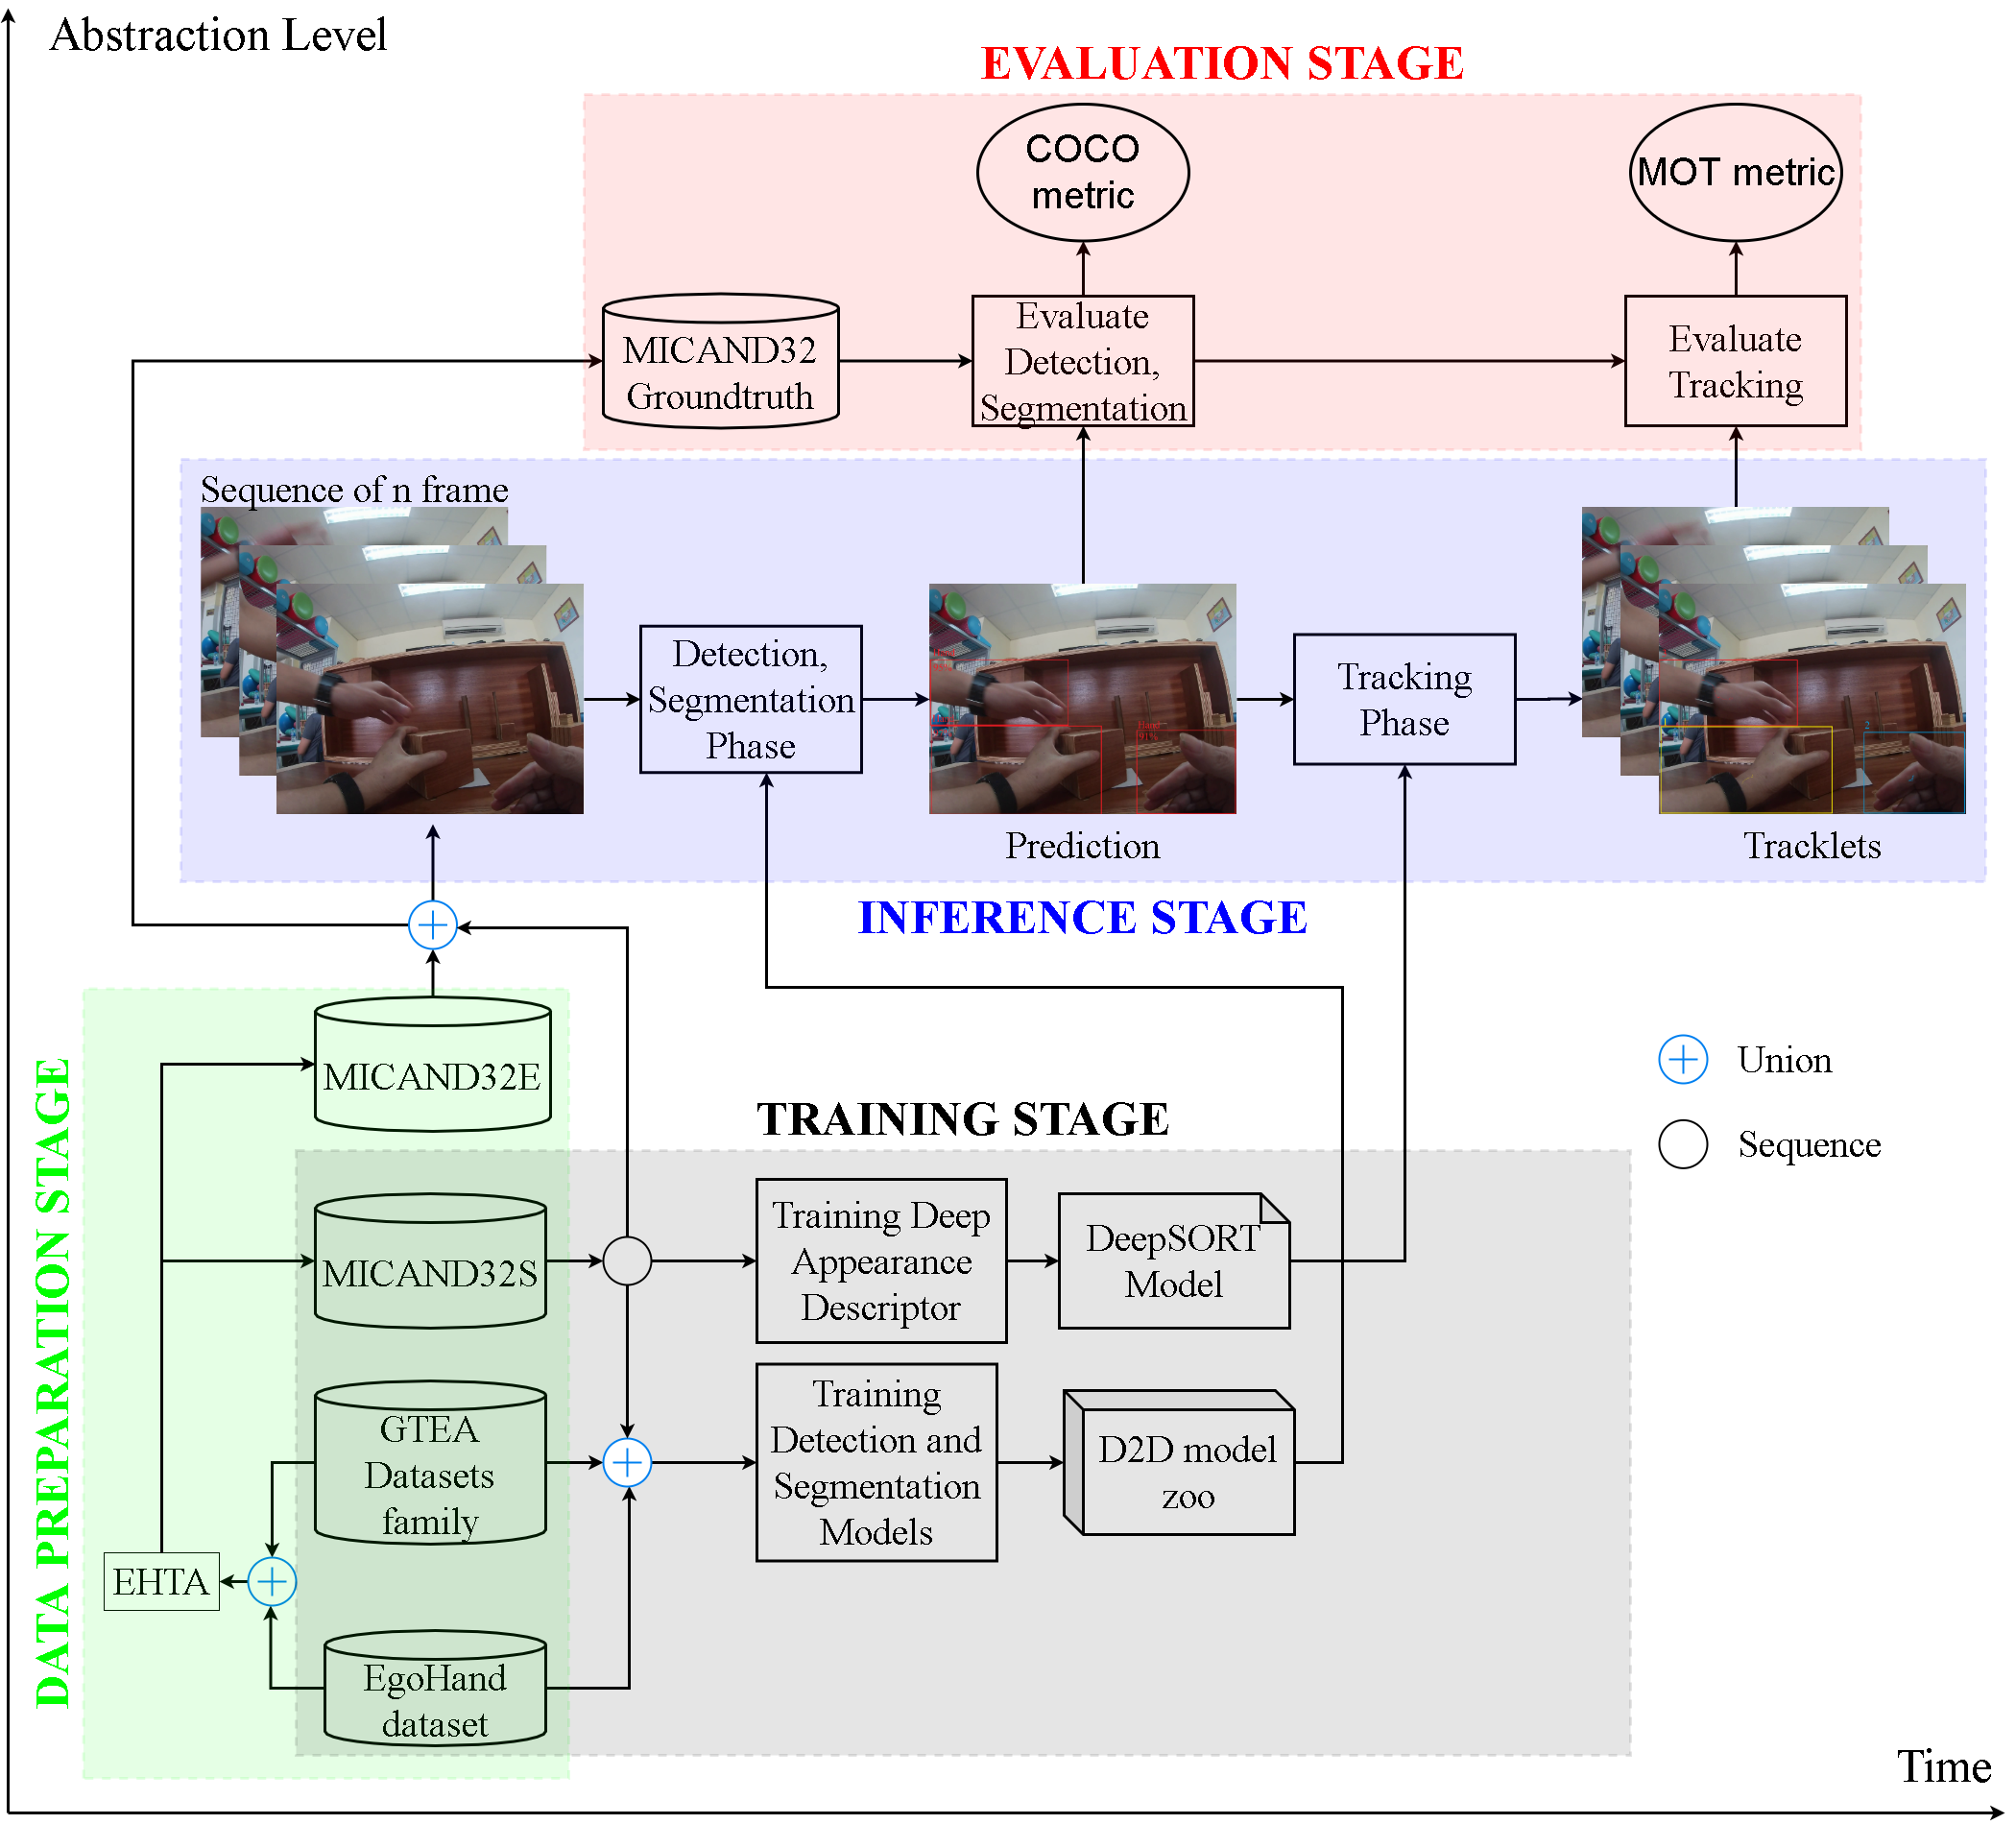
\includegraphics[width=1\linewidth]{Figs/proposedFramework.png}}
	\caption{Overview of proposed framework: D2D. The x-axis represents the time flow of the 4 stages. The y-axis regards the increasing degree of abstraction level of the stages.}
	\label{fig:framework}
\end{figure}
The framework proposed in this thesis consists of 4 stages: \begin{enumerate*}
	\item data preparation stage,
	\item training stage,
	\item inference stage,
	\item evaluation stage
\end{enumerate*}. Initializing with data preparation stage, the GTEA family and EgoHands datasets is collected and is pre-processed in order to keep only suitable and related ground-truth samples. These 2 datasets are used to construct EHTA model zoo by training hand detection and segmentation models from the first-person view. The annotators use semi-automatic EHTA tool to create the new dataset Micand32 descripted in chapter \ref{chap:method}, sub-section \ref{subsec:micand32}. Next is the models training stage. Three datasets including Micand32S, GTEA family and EgoHands datasets is used as fuel to train the hand detection and segmentation from egocentric vision, family of RCNN models and family of YOLO models. At the same time, a deep appearance descriptor is trained on distinct hand groups ground-truth in Micand32S. While the original DeepSORT's descriptor is made in people tracking context, the descriptor trained in the thesis is made well suited for deep metric learning in this egocentric hand context. Detail training techniques are reported in section \ref{sec:trainingstage}. Following the training stage is the inference stage in which all the videos in Micand32 datasets is tested. For each sequence of n frames, each frame in turn is fed respectively into the detection and segmentation phase to get the prediction which locate the hand’s bounding boxes, masks and their confidence scores. This phase requires user to select detection or segmentation algorithm from pre-trained D2D model zoo. Frames with detections are then fed into tracking phase. This phase also requires user to choose tracking algorithm SORT or DeepSORT. The tracking phase indicates the identifications of egocentric hands with their trajectories in the whole video. Section \ref{sec:inferstage} explains in detail the inference procedure. Finally, the evaluation stage encounters. Detection bounding boxes and segmentation masks is be evaluated by comparing with Micand32’s ground-truth. This result is measured in COCO format. The hand’s tracklets is evaluated and reported in MOT Challenge format. Detail evaluation criteria is described in section \ref{sec:evacri}. 
\section{Training stage} \label{sec:trainingstage}
\begin{figure}[htbp]
	\centerline{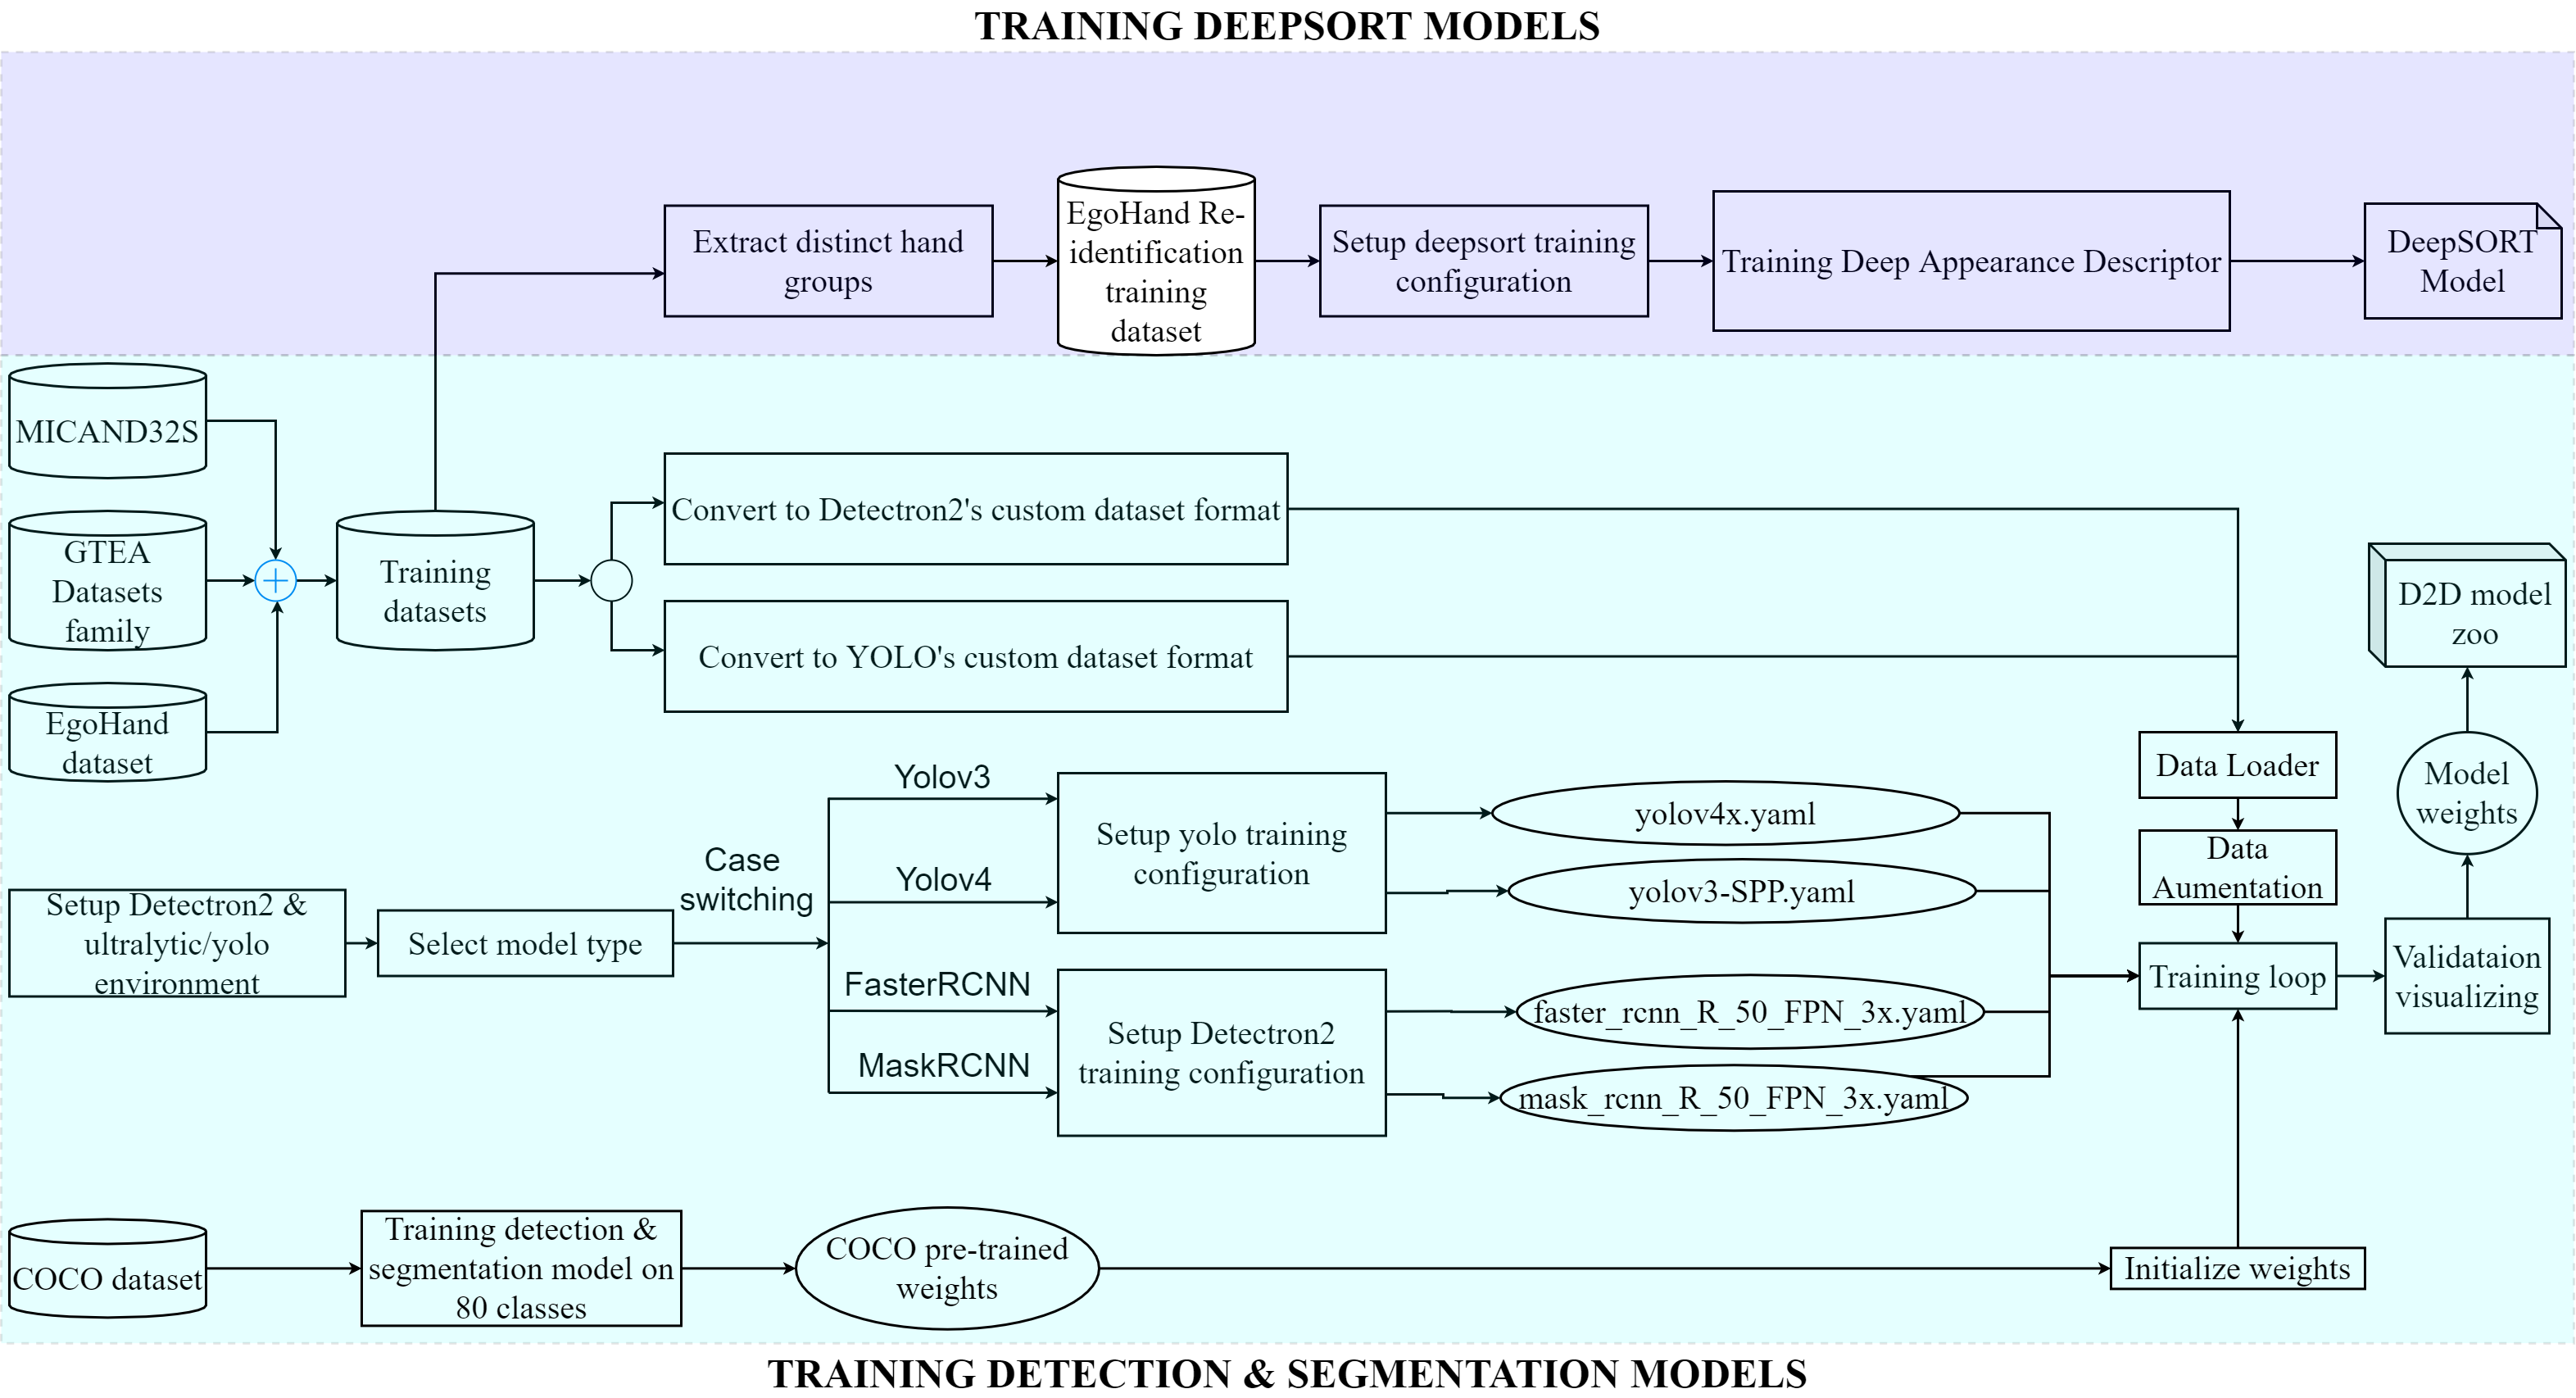
\includegraphics[width=1\linewidth]{Figs/trainingStage.png}}
	\caption{Workflow of the training stage.}
	\label{fig:trainingstage}
\end{figure}
The training stage shown in \ref{fig:trainingstage} consist of parts: \begin{enumerate*}
	\item training detection and segmentation models,
	\item training DeepSORT model
\end{enumerate*}. Input of both parts are the combination of 3 datasets: Miand32S, GTEA family and EgoHands dataset. The first part will generate D2D model zoo which consists 4 types of models, 2 from yolo family and 2 from RCNN family. The second part trains a CNN for deep appearance descriptor for cosine metric learning \cite{DBLP:journals/corr/abs-1812-00442} in DeepSORT. Detail implementation is explained as follow.
\subsection{Training detection and segmentation models}
Initially I setup programming environment which consists 2 frameworks: Detectron2 \cite{wu2019detectron2} for RCNN model family and Ultralytics \cite{ultralytics} for YOLO model family.

Detectron2 is a complete rewrite of the previous version Detectron, and it originates from maskrcnn-benchmark. The platform is now implemented in and powered by the PyTorch deep learning framework. Through a new modular design, Detronron2 is flexible and scalable, and can provide fast training on a single or multiple GPU servers. Detectron2 includes high-quality implementations of state-of-the-art object detection algorithms, including DensePose, panoptic feature pyramid networks, and numerous variants of the pioneering Mask R-CNN model family also developed by FAIR. Its scalable design makes it easy to implement cutting-edge research projects without having to spend the entire code base. The requirements of installing Detectron2 includes: Linux with Python 3.6+, Pytorch 1.4+ and torchvision that matches the PyTorch installation, OpenCV need by demo and visualization. In this thesis, I build Detectron2 from source. The compilers gcc and g++ version 5+ are required, and ninja is recommended for faster build. After having these prerequisites, I clone the Detectron2 repositories and install it via pip from the local clone.

The Ultralytics open-source research into future object detection methods is represented via this repository \cite{ultralytics}. The requirements of install Ultralytics is Python 3.8 or later with all dependencies includes Cython, matplotlib, numpy, OpenCV, pillow, PyYAML, scipy, tensorboard, tqdm, pycocotools, scikit-learn, seaborn, coremltools and onnx. I build Ultralytics from source by cloning their github repository and install via pip.

After installing programming environments, users have to select the model type to train. There are 4 main models integrated in this thesis's framework, the RCNN family consists FasterRCNN and MaskRCNN, while the YOLO family consists Yolov3 and Yolov4. Depending on case of model selection, D2D switches to appropriate branch of setting up training configurations. For the RCNN family, Detectron2 supports different backbone network architectures such as ResNET \{50, 101, 152 \}|, FPN, VGG16, etc. In this thesis, I choose the standard configs, FasterRCNN\_R\_50\_FPN\_3x and MaskRCNN\_R\_50\_FPN\_3x with backbone Resnet 50 layers, feature pyramid network 3x architecture. The config file is saved in a ".yaml" format file. Table \ref{tab:fastConfig} represents a typical configuration for FasterRCNN\_R\_50\_FPN\_3x.

\begin{table}[]
	\label{tab:fastConfig}
	\begin{tabular}{|l|l|}
		\hline
		Key            & Value                                           \\ \hline
		\_BASE\_:      & "../Base-RCNN-FPN.yaml"                         \\ \hline
		MODEL:         &                                                 \\ \hline
		WEIGHTS:       & "detectron2://ImageNetPretrained/MSRA/R-50.pkl" \\ \hline
		MASK\_ON       & False                                           \\ \hline
		RESNETS:       &                                                 \\ \hline
		DEPTH:         & 50                                              \\ \hline
		OUT\_FEATURES: & {[}"res2", "res3", "res4",   "res5"{]}          \\ \hline
		FPN:           &                                                 \\ \hline
		IN\_FEATURES:  & {[}"res2", "res3", "res4",   "res5"{]}          \\ \hline
		SOLVER:        & \multirow{2}{*}{(210000, 250000)}               \\ \cline{1-1}
		STEPS:         &                                                 \\ \hline
		MAX\_ITER:     & 270000                                          \\ \hline
		ROI\_HEADS:    & \multirow{2}{*}{"StandardROIHeads"}             \\ \cline{1-1}
		NAME:          &                                                 \\ \hline
		IN\_FEATURES:  & {[}"p2", "p3", "p4",   "p5"{]}                  \\ \hline
	\end{tabular}
	\caption{FasterRCNN\_R\_50\_FPN3x training configuration file. Detail information field is explained at the Detectron2's application programming interface (API) documentation. The main difference of FasterRCNN and MaskRCNN in term of configuration is MaskRCNN's option MASK\_ON value.}
\end{table}
For the YOLO family, Ultralytics supports different model checkpoints type, and in this thesis, I choose the standard YOLOv3-SPP and YOLOv4x. Training configuration is also saved in a “.yaml” format file. Table \ref{tab:yoloConfig} represents a typical configuration for Yolov4x.
\begin{table}[]
	\label{tab:yoloConfig}
	\begin{tabular}{|l|l|}
		\hline
		Key              & Value                                                                                                                                                                                                                                                                                                                                                                                                                                                                                                                                                                                                                                                                                                                                                                                                                                                                                                                                                                           \\ \hline
		nc:              & 1 \# number of classes                                                                                                                                                                                                                                                                                                                                                                                                                                                                                                                                                                                                                                                                                                                                                                                                                                                                                                                                                          \\ \hline
		depth\_multiple: & 0.33 \# model depth multiple                                                                                                                                                                                                                                                                                                                                                                                                                                                                                                                                                                                                                                                                                                                                                                                                                                                                                                                                                    \\ \hline
		width\_multiple: & 0.50 \# layer channel multiple                                                                                                                                                                                                                                                                                                                                                                                                                                                                                                                                                                                                                                                                                                                                                                                                                                                                                                                                                  \\ \hline
		anchors:         & \begin{tabular}[c]{@{}l@{}}- {[}10,13, 16,30, 33,23{]}  \# P3/8\\ - {[}30,61, 62,45, 59,119{]}  \# P4/16\\ - {[}116,90, 156,198, 373,326{]}  \# P5/32\end{tabular}                                                                                                                                                                                                                                                                                                                                                                                                                                                                                                                                                                                                                                                                                                                                                                                                              \\ \hline
		backbone:        & \begin{tabular}[c]{@{}l@{}}\# {[}from, number, module, args{]}\\   {[}{[}-1, 1, Focus, {[}64, 3{]}{]},  \# 0-P1/2\\    {[}-1, 1, Conv, {[}128, 3, 2{]}{]},  \# 1-P2/4\\    {[}-1, 3, BottleneckCSP, {[}128{]}{]},\\    {[}-1, 1, Conv, {[}256, 3, 2{]}{]},  \# 3-P3/8\\    {[}-1, 9, BottleneckCSP, {[}256{]}{]},\\    {[}-1, 1, Conv, {[}512, 3, 2{]}{]},  \# 5-P4/16\\    {[}-1, 9, BottleneckCSP, {[}512{]}{]},\\    {[}-1, 1, Conv, {[}1024, 3, 2{]}{]},  \# 7-P5/32\\    {[}-1, 1, SPP, {[}1024, {[}5, 9, 13{]}{]}{]},\\    {[}-1, 3, BottleneckCSP, {[}1024, False{]}{]},  \# 9\\   {]}\end{tabular}                                                                                                                                                                                                                                                                                                                                                                      \\ \hline
		head:            & \begin{tabular}[c]{@{}l@{}}{[}{[}-1, 1, Conv, {[}512, 1, 1{]}{]},\\    {[}-1, 1, nn.Upsample, {[}None, 2, 'nearest'{]}{]},\\    {[}{[}-1, 6{]}, 1, Concat, {[}1{]}{]},  \# cat backbone P4\\    {[}-1, 3, BottleneckCSP, {[}512, False{]}{]},  \# 13\\  \\    {[}-1, 1, Conv, {[}256, 1, 1{]}{]},\\    {[}-1, 1, nn.Upsample, {[}None, 2, 'nearest'{]}{]},\\    {[}{[}-1, 4{]}, 1, Concat, {[}1{]}{]},  \# cat backbone P3\\    {[}-1, 3, BottleneckCSP, {[}256, False{]}{]},  \# 17 (P3/8-small)\\  \\    {[}-1, 1, Conv, {[}256, 3, 2{]}{]},\\    {[}{[}-1, 14{]}, 1, Concat, {[}1{]}{]},  \# cat head P4\\    {[}-1, 3, BottleneckCSP, {[}512, False{]}{]},  \# 20  (P4/16-medium)\\  \\    {[}-1, 1, Conv, {[}512, 3, 2{]}{]},\\    {[}{[}-1, 10{]}, 1, Concat, {[}1{]}{]},  \# cat head P5\\    {[}-1, 3, BottleneckCSP, {[}1024, False{]}{]},  \# 23  (P5/32-large)\\  \\    {[}{[}17, 20, 23{]}, 1, Detect, {[}nc, anchors{]}{]},  \# Detect(P3, P4, P5){]}\end{tabular} \\ \hline
	\end{tabular}
	\caption{YOLOv4x training configuration file. Detail information field is explained at Ultralytic API.}
\end{table}
It should be noted that in this thesis the number of classes for training is 1 class “hand”. The initial weights is pre-trained on COCO dataset with 80 classes. The GTEA datasets family, EgoHands dataset and Micand32S datasets is repored in chapter \ref{chap:method}, section \ref{subsec:micand32}, all of them are merged into 1 training dataset. To let detectron2 know how to obtain a custom dataset, I implement a function that returns the items in training datasets. The standard representation for a dataset is combination of multiple dictionaries, each dictionary contains information about one image. The dictionary may have the following fields:
\begin{table}[]
	\begin{tabular}{|l|l|}
		\hline
		Field         & Meaning                                                                                                                                                                                                                                         \\ \hline
		file\_name    & \begin{tabular}[c]{@{}l@{}}the full path to the image file. Rotation or flipping may   be applied if the\\ image has EXIF metadata.\end{tabular}                                                                                                \\ \hline
		height, width & integer.   The shape of the image.                                                                                                                                                                                                              \\ \hline
		image\_id     & \begin{tabular}[c]{@{}l@{}}(str   or int): a unique id that identifies this image. Required by many\\ evaluators  to identify the images, but a dataset may use it for different\\ purposes.\end{tabular}                                       \\ \hline
		annotations   & \begin{tabular}[c]{@{}l@{}}(list{[}dict{]}): Required by instance detection, segmentation or keypoint\\ detection tasks. Each dict corresponds to annotations of one instance in\\ this image.\end{tabular}                                     \\ \hline
		bbox          & \begin{tabular}[c]{@{}l@{}}(list{[}float{]},   required): list of 4 numbers representing the bounding box of\\ the instance.\end{tabular}                                                                                                       \\ \hline
		bbox\_mode    & \begin{tabular}[c]{@{}l@{}}(int, required): the format of bbox. It must be a member\\  of structures.BoxMode. Currently supports: \\ BoxMode.XYXY\_ABS, BoxMode.XYWH\_ABS.\end{tabular}                                                         \\ \hline
		category\_id  & \begin{tabular}[c]{@{}l@{}}(int,   required): an integer in the range {[}0, num\_categories-1{]} representing\\ the category label. The value num\_categories is reserved to represent the\\ “background” category, if applicable.\end{tabular} \\ \hline
		segmentation  & (list{[}list{[}float{]}{]}   or dict): the segmentation mask of the instance.                                                                                                                                                                   \\ \hline
	\end{tabular}
	\caption{Detectron2’s custom dataset format.}
\end{table}
Ultralytics also requires exporting custom dataset labels to YOLO format, with one “*.txt” file per image. The “*.txt” file specifications are: (1) one row per object; (2) each row is “class x\_center y\_center width height” format; (3) box coordinates must be in normalized xywh format (from 0 - 1). If boxes are in pixels, divide x\_center and width by image width, and y\_center and height by image height; (4) class numbers are zero-indexed. Each image's label file should be locatable by simply replacing “/images/*.jpg” with “/labels/*.txt” in its pathname.
\begin{figure}
	\centerline{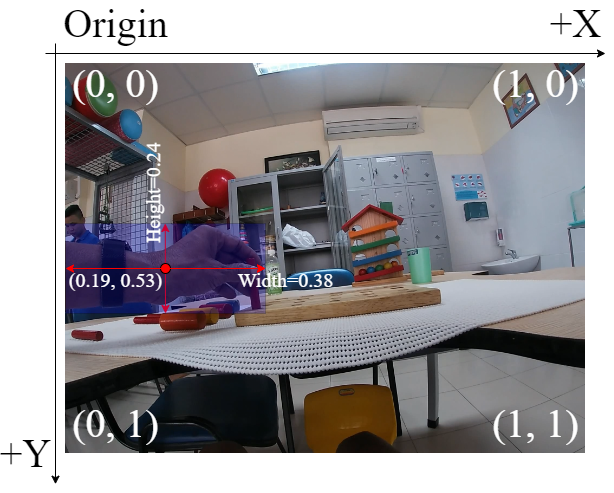
\includegraphics[width=1\linewidth]{Figs/yoloformat.png}}
	\caption{Illustration of YOLO’s data format.}
	\label{fig:yoloformat}
\end{figure}
Data loader is the component that provides data to models. A dataloader usually takes raw information from datasets, and process them into a format needed by the model in training loop. Augmentation is an important part of training. Detectron2’s data augmentation system aims at addressing the following goals: (1) allow augmenting multiple data types together (e.g., images together with their bounding boxes and masks); (2) allow applying a sequence of statically-declared augmentation. For Ultralytics, a Mosaic Dataloader is used for training. The data augmentations used are horizontal and vertical flip, resize, Gauss noise, random brightness contract, crop, median blur, color distortion, gamma, converting color space; some of them are illustrated in \ref{fig:augmentation}.
\begin{figure}
	\centerline{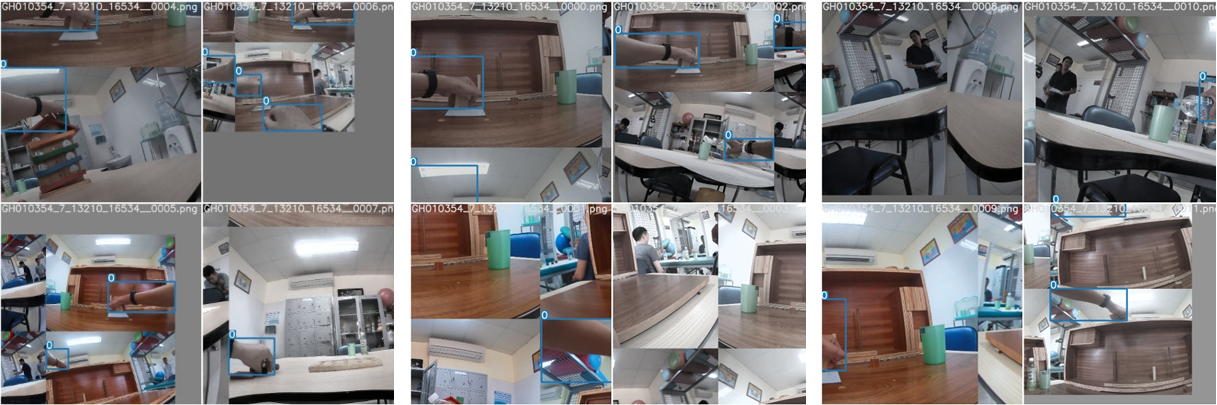
\includegraphics[width=1\linewidth]{Figs/augmentation.png}}
	\caption{Pictorial of data augmentations.}
	\label{fig:augmentation}
\end{figure}
With the benefits of transfer learning techniques discussed in \cite{DBLP:journals/corr/abs-1808-01974}, in this thesis, I start from the pre-trained weights on 80 classes in COCO datasets and fine-tune it for the particular “hand” classes. Training loop runs with defined configurations and augmented data. Table \ref{tab:traintime} reports the training time in this thesis.
\begin{table}[]
	\label{tab:traintime}
	\begin{tabular}{|l|l|}
		\hline
		Model                      & Training   time (hours) \\ \hline
		FasterRCNN\_R\_50\_FPN\_3x & 46                      \\ \hline
		MaskRCNN\_R\_50\_FPN\_3x   & 50                      \\ \hline
		Yolov3\_SPP                & 36                      \\ \hline
		Yolov4x                    & 40                      \\ \hline
	\end{tabular}
	\caption{Training time for detection and segmentation models.}
\end{table}
The visualization of training steps is available via Tensorboard during training time as in \ref{fig:tensorboard}.
\begin{figure}
	\centerline{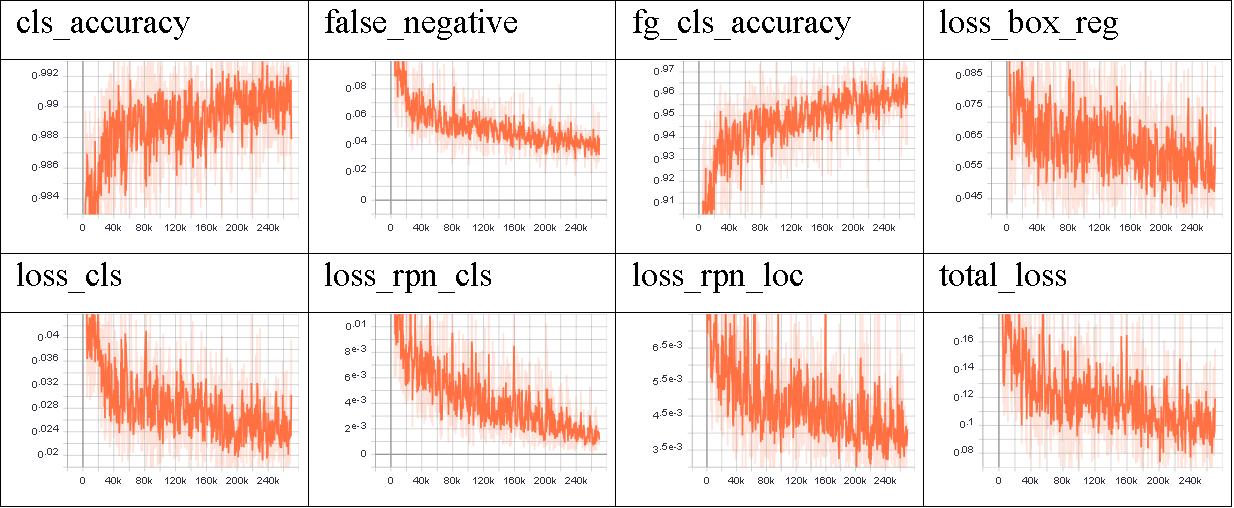
\includegraphics[width=1\linewidth]{Figs/tensorboard.png}}
	\caption{FasterRCNN\_R\_50\_FPN\_3x losses visualization during training time.}
	\label{fig:tensorboard}
\end{figure}
\\After training, the framework generates the D2D model zoo which contains 4 model with corresponding weights save in “.h” data format and will be used in the inference stage.
\subsection{Training Deep Appearance Descriptor for DeepSORT}
The original DeepSORT is used for person tracking task – a familiar issue in which a given query image is used to look at a huge gallery of images that have been gathered at distinct moments, lighting environments, actions performing that may contain the same individual. To customize it on egocentric hand tracking mission, it firstly requires an egocentric hand re-identification dataset to train the appropriate appearance descriptor. As the best of my knowledge, there are very few public egocentric hand re-identification datasets available \cite{9064606}. From the analysis of 3 datasets described in chapter \ref{chap:method}, section \ref{sec:datasets}, I build a new egocentric hand re-identification dataset from the identity information annotations. Images of hands are extracted and cropped from these 3 datasets using the bounding box information and also resized to the same size (100, 100) as recommendation in  \cite{DBLP:journals/corr/abs-1812-00442}. As a result, there are in total 40 identities (26 subject from GTEA + 4 subject from EgoHands + 10 subject from Micand32S = 40 subjects) and 29324 images in this egocentric hand re-identification dataset. The sample of the images used in this dataset is shown in \ref{fig:reid}.
\begin{figure}
	\centerline{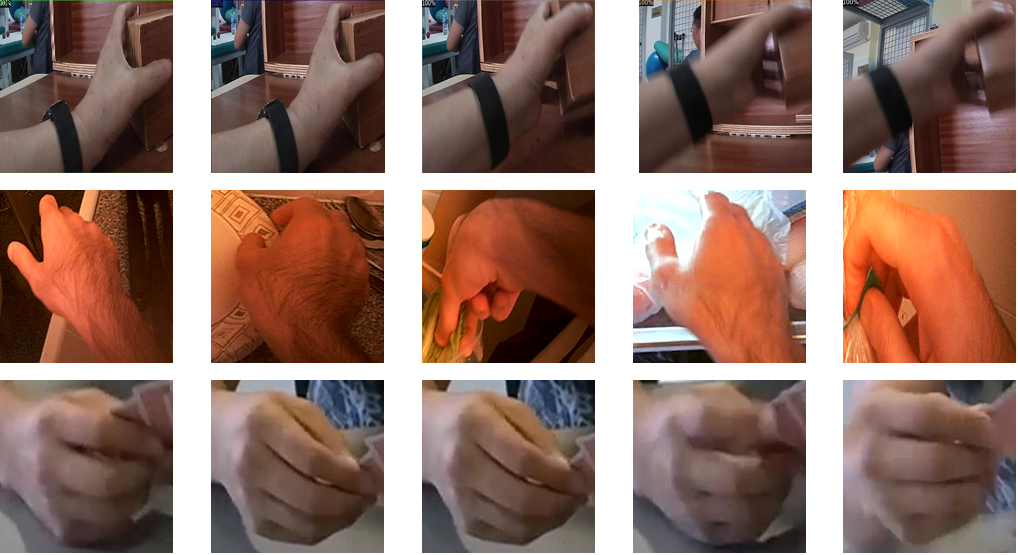
\includegraphics[width=1\linewidth]{Figs/reid.png}}
	\caption{Images from the self-generated egocentric hand re-identification dataset. Images in the same row has the same identity.}
	\label{fig:reid}
\end{figure}
Having obtained the egocentric hand re-identification dataset, I train the CNN to get the appearance descriptor. The train and test sets were slit into 80\% and 20\% respectively and both were structed by place all the images of one identity into a specific numbered folder for both train and test sets. I setup the training configuration as in Table \ref{tab:des}. The programming environment in which the training process performed is python 3 with PyTorch framework, numpy, scipy, sklearn, pillow, vizer and edict package.
\begin{table}	
	\label{tab:des}
	\begin{tabular}{|l|l|}
		
		\hline 
		Field & Value\\ 
		\hline 
		Batch size & 64 \\
		\hline
		No. of epochs & 40 \\
		\hline
		Learning rate & 0.1 \\
		\hline
		Momentum & 0.9 \\
		\hline
		Weight decay & 5e-4\\ 
		\hline
		Learning decay & 0.1 after every 10 epochs\\
		\hline
	\end{tabular} 
\caption{Main training configuration of DeepSORT’s appearance descriptor.}
\end{table}
The training chart obtained is shown in \ref{fig:descriptor}. It tooks 40 hours to train this CNN.
\begin{figure}[htbp]
	\centerline{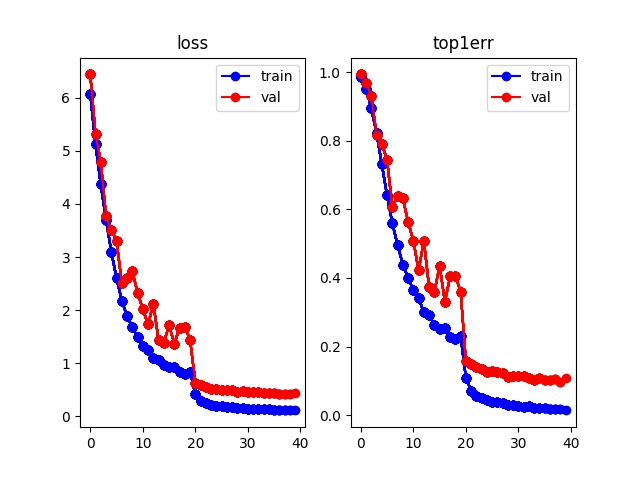
\includegraphics[]{Figs/descriptor.jpg}}
	\caption{Workflow of inference stage.}
	\label{fig:descriptor}
\end{figure}
\section{Inference stage}\label{sec:inferstage}
\begin{figure}[htbp]
	\centerline{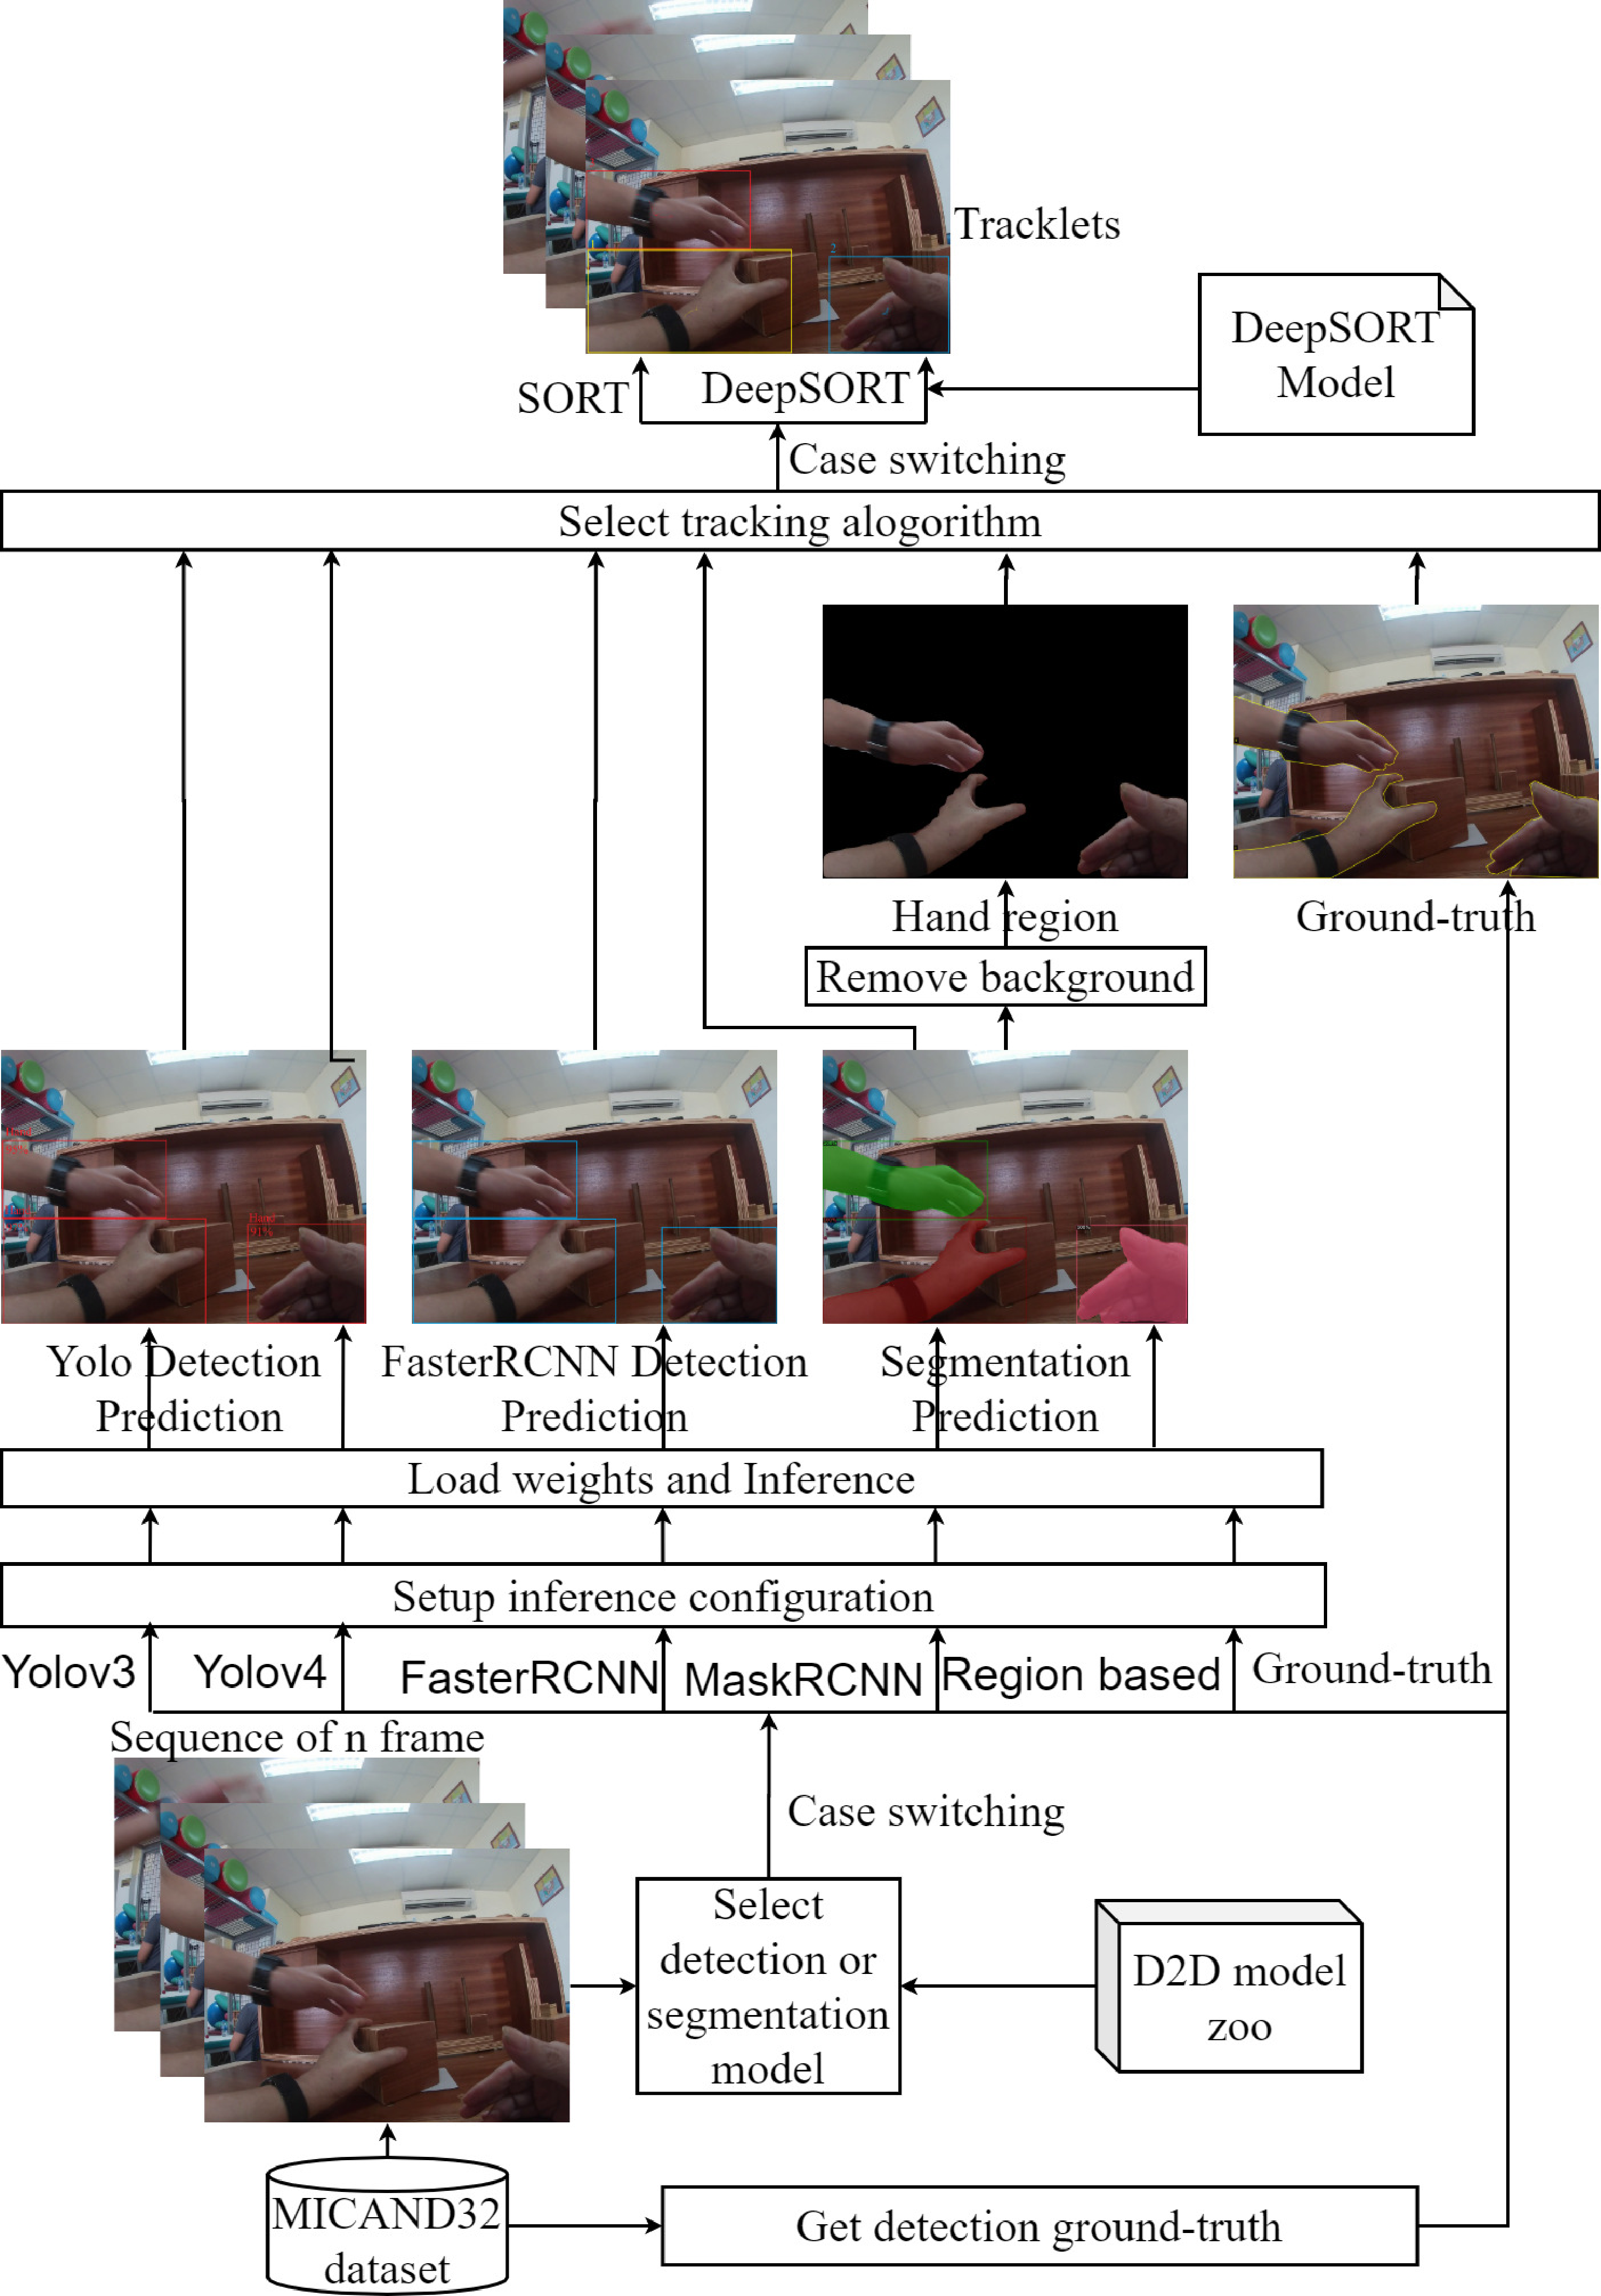
\includegraphics[width=\textwidth]{Figs/inferenceStage.eps}}
	\caption{Workflow of inference stage.}
	\label{fig:inferenceStage}
\end{figure}
In inference stage \ref{fig:inferenceStage}, each of 32 videos from Micand32 dataset will be tested in turn. Initially Each frame is fed into the detection phase in chronological order. Next, users select a detection or segmentation model from the D2D model zoo which was already trained in training stage. In order to analyze the affection of the detection phase on tracking phase, the detection ground-truth of Micand32 is also available for user to select in this step. As a consequence, 6 options are available: Yolov3\_spp, Yolov4x, FasterRCNNR50FPN3x, MaskRCNNR50FPN3x, MaskRCNNR50FPN3x with region based and detection ground-truth. Depending on the chosen model type, the D2D framework will setup inference configurations. For example, the default confidence threshold in this thesis is 50\%. Appropriate pre-trained weights will be loaded from the D2D model zoo in “.h” format and the inference process will begin. For detection models which includes yolo model family and FasterRCNNR50FPN3x, each prediction on image is represented in the following format: \(pred^i = [x_0^i, y_0^i, x_1^i, y_1^i, c^i]\) where \(pred^i\) is the i-th prediction with \((x_0^i, y_0^i),  (x_1^i, y_1^i)\), is respectively the top-left and bottom-right vertex coordinate of the i-th bounding box and ci is the current confident score of this bounding box. For MaskRCNNR50FPN3x, each prediction will consist one more field: \(pred^i = [x_0^i, y_0^i, x_1^i, y_1^i, pol^i, c^i]\) where the \(pol^i\) is the polygon of the mask in RLE format. For MaskRCNNR50FPN3x with region-based option, after obtaining the mask predictions, the framework will execute background subtraction in order to keep only hand region. This is intended to make the deep appearance descriptor in DeepSORT focus more on the hand region. In the following step, users will select the tracking algorithm, include: SORT or DeepSORT. For SORT, detection will be processed in Kalman filter and then associated by the Hungarian algorithm as explained in chapter 2, section 2.3. For DeepSORT, the deep appearance descriptor will be loaded from the pre-trained CNN in the training stage. Tracklets for the whole sequences will be compared with the tracking ground-truth in evaluation stage in order to analyze the effective of the algorithms.
\section{Evaluation stage}
Detail evaluation criteria and measurement metrics is reported in chapter \ref{chap:exp}, section \ref{sec:evacri}. The evaluation stage includes 2 parts: (1) evaluate detection and segmentation results; (2) evaluate tracking results. For detection and segmentation result, this thesis adopts the evaluation API from Detectron2 repository and the py-cocotools package. For tracking result, performance is measured according to the framework presented in \cite{DBLP:journals/corr/MilanL0RS16}. The authors provide evaluation scripts for official development kit of MOT Challenge. MOT16 was chosen since it is a compilation of other many metrics developed in an attempt to standardize evaluation of multiple object tracking. This devkit requires Python 3.7+, Matlab R2020a, matlab python engine, pandas and pytz. Tracking result will be saved in simple comma-separated value (CSV) files. Each line represents one object instance and contains 9 values as show in Table 3 6. 
\begin{table}	
	\label{tab:des}
	\begin{tabular}{|l|l|p{9cm}|}
		
		\hline 
		Position & Name & Description\\ 
		\hline 
		1 & Frame number & Indicate at which frame the object is present\\
		\hline
		2 & Identity number & Each hand trajectory is identified by a unique ID\\
		\hline
		3 & Bounding box left & Coordinate of the top-left corner of the pedestrian bounding box\\
		\hline 
		4 & Bounding box top & Coordinate of the top-left corner of the pedestrian bounding box\\
		\hline
		5 & Bounding box width & Width in pixels of the hand bounding box\\
		\hline
		6 & Bounding box height & Height in pixels of the hand bounding box\\
		\hline 
		7 & Confidence score & It acts as a flag whether the entry is to be considered (1) or ignored (0)\\
		\hline
		8 & Class & Indicates the type of object annotated. In this thesis, always (1)\\
		\hline
		9 & Visibility & Visibility ratio, a number between 0 and 1 that says how much of the hand is visible. Can be due to occlusion and due to image border cropping.\\
		\hline
	\end{tabular} 
	\caption{Data format for both the inference result and ground-truth annotation of tracking \cite{DBLP:journals/corr/MilanL0RS16}.}
\end{table}
An example of such an annotation file is:
\begin{itemize}
	\item 1, 1, 1672, 763, 248, 245, 1, 1 ,1
	\item 1, 2, 1253, 426, 156, 200, 1, 1 ,1
	\item 2, 1, 1668, 774, 252, 234, 1, 1, 1
\end{itemize}
In this case, there are 2 hand in the first frame of the sequence, with identity tags 1, 2 and 1 hand in the second frame with identity tags 1.
%% This is an example first chapter.  You should put chapter/appendix that you
%% write into a separate file, and add a line \include{yourfilename} to
%% main.tex, where `yourfilename.tex' is the name of the chapter/appendix file.
%% You can process specific files by typing their names in at the 
%% \files=
%% prompt when you run the file main.tex through LaTeX.
\chapter{Experiments}\label{chap:exp}

\section{Evaluation criteria} \label{sec:evacri}
\subsection{Object detection evaluation metrics}
Average Precision is a standard and popular metric in measuring the performance of the object detection and segmentation algorithms. The Precision (Prcn) and Recall (Rcll) are defined as follow:
\begin{equation}
	Prcn = \frac{TP}{TP+FP}
\end{equation}
\begin{equation}
	Rcll = \frac{TP}{TP+FN}
\end{equation}
where, TP, FP, and FN are number of True Positive, False Positive, and False Negative, respectively. A predicted bounding box is considered a TP if its intersection over union (IoU), or Jaccard Index, with a ground truth box is larger than 0.5. Equation \ref{eq:IoU} shows how the IoU between a predicted box P and a ground truth box G is calculated.
\begin{equation}
	\label{eq:IoU}
	IoU(P,G) = \frac{|P\cap G|}{| P \cup G |}
\end{equation}
F1 score is a metric that combines recall and precision into a single score by calculating the harmonic mean of precision and recall:
\begin{equation}
	F1 = \frac{2TP}{2TP+FP+FN}
\end{equation}
Latest research papers tend to give results in the COCO dataset format. In COCO mAP, a 101-point interpolated AP definition is used in the calculation. For COCO, AP is the average over multiple IoU. AP@[. 5: .95] corresponds to the average AP for IoU from 0.5 to 0.95 with a step size of 0.05. The following are some other metrics collected for the COCO dataset:
\subsection{Object tracking evaluation metrics}
Performance is measured according to the framework presented in MOT16 \cite{DBLP:journals/corr/MilanL0RS16} and in the same manner as performance is measure in the MOTChallange. The authors of \cite{DBLP:journals/corr/MilanL0RS16} provide publicly available code for evaluation, this code is used to calculate the different performance metrics. MOT16 was chosen since it is a compilation of other many metrics developed in an attempt to standardize evaluation of multiple object tracking. MOT16 contains a wide array of metrics for evaluation of multiple object tracking, some which are quite similar to each other. Hence, metrics that were considered to similar to other have not been included in this thesis.
\begin{itemize}
	\item Identification Recall (IDR) and Identification Precision (IDP): IDR and IDP are similar to the metrics Recall and Precision for object detection. The metrics will however differ since objects are considered tracked only if they can be assigned an identity, which will not be the case for all detected objects. Another difference is that inconsistencies in identity assignments will lower the IDTP score. For each ground truth identity, the predicted identity most similar to it is found. Any other identity assigned to the ground truth identity is then considered a mismatch (IDFP) and will be counted as a false positive instead of a true positive.
	\begin{equation}
		IDR = \frac{IDTP}{IDTP+IDFP}
	\end{equation}
	\begin{equation}
		IDP = \frac{IDTP}{IDTP+IDFN}
	\end{equation}
where, IDTP is the sum of TP in detection and the number of correctly labeled objects in the tracking; IDFP/IDFN is the sum of FP/FN in detection and the number of correctly predicted objects for positive class in detection but incorrectly labeled in tracking.
	\item IDF1-score(IDF1): Similar to F1 score for object detection, IDF1 combines both IDR and IDP into a single score to facilitate comparisons of different trackers. The higher IDF1 is, the better tracker is.
	\begin{equation}
		IDF1 = \frac{2IDTP}{2IDTP+IDFP+IDFN}
	\end{equation}
	\item Mostly Tracked (MT): The number of ground truth identities that are tracked for 80\% or more of their existence.
	\item Partly Tracked (PT): The number of ground truth identities that are tracked between 20\% and 80\% of their existence.
	\item Mostly Lost (ML): The number of ground truth identities that are tracked for less than 20\% of their existence.
	\item Identity Switches (IDs): The number of identity switches. An identity switch is counted every time an already tracked ground truth identity is assigned a new tracking identity.
	\item Track Fragmentations (FM): The number of track fragmentations. A track fragmentation is counted every time a tracked ground truth identity is lost and then found again in a later frame.
	\item Multiple Object Tracking Accuracy (MOTA): MOTA combines false negatives, false positives and identity switches into a single score in order to express overall performance with a single value. This is the most important metric for object tracking evaluation and it is defined as:
	\begin{equation}
		MOTA = 1 - \frac{\sum _t (IDFN_t+IDFP_t+IDS_t)}{\sum _t GT_t}
	\end{equation}
where, t is the index of frame, GT is the number of observed objects in the real-world. It is worth to note that MOTA would be a negative value if there are many errors in the tracking process and the number of these errors is larger than that of observed objects.
	\item Multiple Object Tracking Precision(MOTP): MOTP measures how well correctly predicted bounding boxes TP fit their respective ground truth boxes GT. This is done by calculating the average overlap between true positives and their corresponding ground truth object.
	\begin{equation}
		MOTP = \frac{\sum _t d_{t,i}}{\sum _t c_t}
	\end{equation}
where, \(c_t\) denotes the number of matches found in the frame t and \(d_{t,i}\) is the sum of distances between all true positive and their corresponding ground truth i. This metric indicate the ability of the tracking in estimating precise object positions.
\end{itemize}
\section{Experimental results}
The following sub-sections will present result for different object detection and tracking algorithms tested in this thesis. All experiments are conducted on 32 videos of Micand32 datasets. The average inference speed is measured on a Workstation super-micro with Intel® Xeon®, CPU E5-2620 v2@2.1GHz, 6 cores, 12 threads, RAM 12GB, GPU GTX 1080.
\subsection{Egocentric hand detection and segmentation result}\label{subsec:det_res}
This subsection presents results for the different object detection algorithms consider in this thesis. The algorithms to be evaluated are: Yolov3\_spp, Yolov4x, FasterRCNN\_R\_50\_FPN\_3x, MaskRCNN\_R\_50\_FPN\_3x. Detection evaluation is show in Table \ref{tab:detres_ap}, Table \ref{tab:detres_ar} and Table \ref{tab:detres_sp}.
\begin{table}[]
	\centering
	\label{tab:detres_ap}
	\caption{Object detection and segmentation Average Precision following the COCO standard.}
	\begin{tabular}{|c|c|c|c|c|c|c|}
		\hline
		Algorithm                  & AP            & AP50          & AP75          & \(AP^{small}\) & \(AP^{medium}\)      & \(AP^{large}\)       \\ \hline
		Yolov3                & 89.2          & 92.4          & 92.1          & 1.1     & 66.4          & 54.1          \\ \hline
		Yolov4x                    & 93.1          & 95.6          & 94.6          & 3.2     & 72.5          & 42.9          \\ \hline
		FasterRCNN & \textbf{96.2} & 97.9          & \textbf{97.9} & 0.9     & \textbf{75.8} & 6.3           \\ \hline
		MaskRCNN  & 92.1          & \textbf{98.9} & 97.9          & 0.0     & 32.4          & \textbf{92.2} \\ \hline
	\end{tabular}
\end{table}
\begin{table}[]
	\centering
	\caption{Object detection and segmentation Average Recall following the COCO standard.}
	\label{tab:detres_ar}
	\resizebox{\textwidth}{!}{%
		\begin{tabular}{|c|c|c|c|c|c|c|}
			\hline
			Algorithm                  & \(AR^{max=1}\)      & \(AR^{max}=10\)      & \(AR^{max}=100\)     & \(AR^{small}\) & \(AR^{medium}\)      & \(AR^{large}\)       \\ \hline
			Yolov3                & 6.5          & 53.6          & 76.4          & 3.2     & 32.5          & 75.9          \\ \hline
			Yolov4x                    & 8.7          & 65.8          & 89.7          & 7.1     & 40.1          & 82.7          \\ \hline
			FasterRCNN & \textbf{9.6} & 76.8          & \textbf{97.6} & 10.0    & \textbf{77.8} & \textbf{97.6} \\ \hline
			MaskRCNN   & 9.2          & \textbf{73.9} & 94.6          & 0.0     & 50.8          & 94.7          \\ \hline
		\end{tabular}%
	}
\end{table}
\begin{table}[hbt!]
	\centering
	\caption{Object detection and segmentation average training and inference time, speed and machine requirements.}
	\label{tab:detres_sp}
	\resizebox{\textwidth}{!}{%
		\begin{tabular}{|c|c|c|c|c|c|}
			\hline
			\multirow{2}{*}{Algorithm} & \multicolumn{2}{l|}{Average time}         & \multirow{2}{*}{Speed (Hz)} & \multicolumn{2}{l|}{Memory requirement (MB)} \\ \cline{2-3} \cline{5-6} 
			& Training (hour) & Inference (millisecond) &                             & RAM                   & GPU                  \\ \hline
			Yolov3                & \textbf{36}     & 45                      & 22                          & \textbf{1989}         & 2260                 \\ \hline
			Yolov4x                    & 40              & \textbf{38}             & \textbf{25}                 & 2152                  & \textbf{2076}        \\ \hline
			FasterRCNN & 46              & 84                      & 12                          & 2351                  & 3297                 \\ \hline
			MaskRCNN   & 50              & \textbf{215}            & \textbf{5}                  & \textbf{2461}         & \textbf{3674}        \\ \hline
		\end{tabular}%
	}
\end{table}
\subsection{Egocentric hand tracking result}
Tracking results for SORT and DeepSORT with different object detection strategy are presented in this section. As described in section 3.4, the tests are performed in a tracking by detection system where tracking and detection algorithms are completely separated. Therefore, different results for combinations of tracking and detection algorithms are reported. Further, ground-truth detection are also test with SORT and DeepSORT. This is done so as to give an insight how much of the error is due to the object detection algorithm and how much of it is due to the tracking algorithm. Tracking performance with ground-truth detection should only have errors introduced by the tracking algorithms and can thereby give an upper limit for how much better the tracking by detection system can become by changing object detection algorithm. Thus, this frameworks consists of 6 detction and segmentation algorithms, they are: Yolov3\_SPP, Yolov4x, Faster\_RCNN\_R\_50\_FPN\_3x, Mask\_RCNN\_R50\_FPN\_3x, Mask\_RCNN\_R50\_FPN\_3x with region based and detection ground-truth. Their combination with 2 tracking algorithms, SORT and DeepSORT, we obtain a total of 12 options for the pipeline. However, the combination of MaskRCNN with region based and SORT scheme is identical to the combination of Mask and SORT scheme because in theory, the SORT algorithm does not use visual information fields. To conclude, we have 11 approaches conventionally defined as in the Table \ref{tab:notation} for brief presentation.
\begin{table}[]
	\centering
	\label{tab:notation}
	\caption{Notation of the 11 approaches mentioned and used in the experiments.}
	\begin{tabular}{|l|l|c|l|}
		\hline
		No & Detector              & Tracker                                        & Notation \\ \hline
		1  & Yolov3                & \multirow{5}{*}{SORT}                          & Y3S      \\ \cline{1-2} \cline{4-4} 
		2  & Yolov4                &                                                & Y4S      \\ \cline{1-2} \cline{4-4} 
		3  & FasterRCNN            &                                                & FS       \\ \cline{1-2} \cline{4-4} 
		4  & MaskRCNN              &                                                & MS       \\ \cline{1-2} \cline{4-4} 
		5  & Groundtruth           &                                                & GS       \\ \hline
		6  & Yolov3                & \multicolumn{1}{c|}{\multirow{6}{*}{DeepSORT}} & Y3DS     \\ \cline{1-2} \cline{4-4} 
		7  & Yolov4                & \multicolumn{1}{c|}{}                          & Y4DS     \\ \cline{1-2} \cline{4-4} 
		8  & FasterRCNN            & \multicolumn{1}{c|}{}                          & FS       \\ \cline{1-2} \cline{4-4} 
		9  & MaskRCNN              & \multicolumn{1}{c|}{}                          & MS       \\ \cline{1-2} \cline{4-4} 
		10 & MaskRCNN+Region based & \multicolumn{1}{c|}{}                          & RDS      \\ \cline{1-2} \cline{4-4} 
		11 & Groundtruth           & \multicolumn{1}{c|}{}                          & GDS      \\ \hline
	\end{tabular}
	\vspace{-0.7cm}
\end{table}
\\In this thesis, I conduct the experiments to evaluate the performance of these approaches on the custom dataset Micand32 which contains 2 sub-datasets: Micand32S and Micand32E. The properties of this dataset is reported in chapter \ref{chap:method}, sub-section \ref{subsec:micand32}.
\subsubsection{Short-term tracking on a standard dataset: Micand32S}
The Mican32S sub-datasets contains 26 sequences containing in total 3162 frames as per the MOT16 Challenge rules and recommendations, each containing from 100 to 300 images. These recordings are chosen so every video has an excursion span of precisely one patient’s activity, for instance opening the cap of the water bottle, getting the circle, playing with the ball, turning left of right, etc. Simultaneously, every video generally contains just 1 or 2 active hands. This sub-dataset can be characterized into short-term tracking datasets. The desire set for the framework proposed in this theory is to recognize, segment, and track this entire fundamental excursion of the hand. Since the quantity of recordings is up to 26 recordings, in this part I will list the overall evaluation for each approach on the whole 26 recordings, which is a weighted average of the quantity of frames per video. Besides, I likewise measure a case of 26 recordings running on 1 approach to see the impact of the sort of activity on the presentation of the framework. Note that the hand in the 26 recordings is utilized to train the deep appearance descriptor for DeepSORT as referenced in chapter \ref{chap:framework}, sub-section \ref{subsec:train_deep}. Table \ref{tab:short_overall} reports short-term tracking overall result on Micand32S following the MOT16 evaluation protocol.
\begin{table}[]
	\caption{Short-term tracking \textbf{overall} result on Micand32S following the MOT16 evaluation protocol.}
	\label{tab:short_overall}
	\centering
	\resizebox{\textwidth}{!}{%
		\begin{tabular}{|l|l|l|l|l|l|l|l|l|l|l|l|l|l|l|l|}
			\hline
			Method & \begin{tabular}[c]{@{}l@{}}IDF1\\ (\%)$\uparrow$­\end{tabular} & 
			\begin{tabular}[c]{@{}l@{}}IDP\\ (\%)$\uparrow$­\end{tabular} & 
			\begin{tabular}[c]{@{}l@{}}IDR\\ (\%)$\uparrow$­\end{tabular} & 
			\begin{tabular}[c]{@{}l@{}}Rcll\\$\uparrow$    ­\end{tabular} & 
			\begin{tabular}[c]{@{}l@{}}Prcn\\$\uparrow$    ­\end{tabular} & 
			\begin{tabular}[c]{@{}l@{}}GT\\$\uparrow$      ­\end{tabular} & 
			\begin{tabular}[c]{@{}l@{}}MT\\$\uparrow$      ­\end{tabular} & 
			\begin{tabular}[c]{@{}l@{}}PT\\$\uparrow$      ­\end{tabular} &
			\begin{tabular}[c]{@{}l@{}}ML\\$\downarrow$     \end{tabular} &
			\begin{tabular}[c]{@{}l@{}}FP\\$\downarrow$     \end{tabular} &        
			\begin{tabular}[c]{@{}l@{}}FN\\$\downarrow$     \end{tabular} &         
			\begin{tabular}[c]{@{}l@{}}IDs\\$\downarrow$     \end{tabular} &        
			\begin{tabular}[c]{@{}l@{}}FM\\$\downarrow$     \end{tabular} &         
			\begin{tabular}[c]{@{}l@{}}\textbf{MOTA}\\ (\%)$\uparrow$­\end{tabular} &
			\begin{tabular}[c]{@{}l@{}}MOTP\\ $\downarrow$­\end{tabular}            \\ \hline
			Y3S    & 97.0                                                 & 99.6                                                & 94.6                                                & 94.8                                                   & 99.8                                                   & 35                                                   & 33          & \textbf{1}                                           & 1          & 6          & 207        & 1          & 1          & 94.6                                                 & 0.087          \\ \hline
			Y4S    & 98.6                                                 & 99.4                                                & 97.7                                                & 97.8                                                   & 99.4                                                   & 35                                                   & \textbf{34} & \textbf{1}                                           & \textbf{0} & 23         & 89         & \textbf{0} & 5          & 97.2                                                 & 0.108          \\ \hline
			FS     & 97.1                                                 & 99.7                                                & 94.6                                                & 94.8                                                   & 99.9                                                   & 35                                                   & 33          & \textbf{1}                                           & 1          & 4          & 206        & 1          & 1          & 94.7                                                 & 0.087          \\ \hline
			MS     & 98.8                                                 & 99.7                                                & 98.0                                                & 98.2                                                   & 99.9                                                   & 35                                                   & 34          & \textbf{1}                                           & \textbf{0} & 3          & 73         & 1          & 1          & 98.1                                                 & 0.072          \\ \hline
			GS     & \textbf{99.9}                                        & 99.9                                                & \textbf{99.9}                                       & \textbf{99.9}                                          & \textbf{100.0}                                         & 35                                                   & \textbf{34} & \textbf{1}                                           & \textbf{0} & 1          & 4          & \textbf{0} & \textbf{0} & \textbf{99.9}                                        & 0.089          \\ \hline
			Y3DS   & 97.1                                                 & 99.6                                                & 94.7                                                & 94.9                                                   & 99.8                                                   & 35                                                   & 33          & \textbf{1}                                           & 1          & 7          & 203        & 1          & 2          & 94.7                                                 & 0.088          \\ \hline
			Y4DS   & 98.8                                                 & 99.6                                                & 97.9                                                & 98.1                                                   & 99.8                                                   & 35                                                   & \textbf{34} & \textbf{1}                                           & \textbf{0} & 7          & 74         & 1          & 2          & 97.9                                                 & 0.106          \\ \hline
			FDS    & 98.2                                                 & 99.9                                                & 96.5                                                & 96.5                                                   & \textbf{100.0}                                         & 35                                                   & 33          & \textbf{1}                                           & 1          & 1          & 140        & \textbf{0} & \textbf{0} & 96.5                                                 & 0.077          \\ \hline
			MDS    & 98.2                                                 & 99.9                                                & 96.5                                                & 96.5                                                   & \textbf{100.0}                                         & 35                                                   & 33          & \textbf{1}                                           & 1          & 1          & 140        & \textbf{0} & \textbf{0} & 96.5                                                 & 0.076          \\ \hline
			RDS    & 99.3                                                 & 99.3                                                & 99.3                                                & 99.3                                                   & 99.4                                                   & 35                                                   & \textbf{34} & \textbf{1}                                           & \textbf{0} & 25         & 27         & \textbf{0} & 6          & 98.7                                                 & 0.089          \\ \hline
			GDS    & \textbf{99.9}                                        & \textbf{100}                                        & 99.8                                                & 99.8                                                   & \textbf{100.0}                                         & 35                                                   & \textbf{34} & \textbf{1}                                           & \textbf{0} & \textbf{0} & \textbf{0} & \textbf{0} & 1          & 99.8                                                 & \textbf{0.062} \\ \hline
		\end{tabular}%
	}
\end{table}
The GDS presents an almost perfect performance on Micand32S, detailed metrics of this method is revealed in Figure \ref{fig:GDS_short}. Of all ground-truth-free approaches, the Y4DS approach reaches a remarkable result shown in Figure \ref{fig:y4ds_short}.
\subsubsection{Long-term tracking on a realistic dataset: Micand32E}
In this part, I will validate the effectiveness of the 11 approaches on the Micand32E dataset. As referenced in chapter \ref{chap:method}, sub-section \ref{subsec:micand32}, the Micand32E contains 6 sequences, the sequence length of each is in range of 1000 frames and 2000 frames, and total the volume of this sub-dataset is 7857 frames. Also, this sub-dataset fully contains 4 types of patient’s action: (5) practice with a ball, (6) practice with water bottles, (7) practice with wooden blocks, (8) practice with cylinders. This sub-dataset is very realistic, interesting and quite challenging because it is specifically selected with careful observations  by developers in the NAFOSTED’s project who are experienced in computer vision problems.
Table \ref{tab:long_overall} presents the overall tracking results referenced on Micand32E of the 11 approaches.
% Please add the following required packages to your document preamble:
% \usepackage{graphicx}
% Please add the following required packages to your document preamble:
% \usepackage{graphicx}
\begin{table}[]
	\caption{Long-term tracking \textbf{overrall} results on Micand32E following the MOT16 protocol.}
	\label{tab:long_overall}
	\centering
	\resizebox{\textwidth}{!}{%
		\begin{tabular}{|l|l|l|l|l|l|l|l|l|l|l|l|l|l|l|l|}
			\hline
			Method & \begin{tabular}[c]{@{}l@{}}IDF1\\ (\%)$\uparrow$­\end{tabular} & 
			\begin{tabular}[c]{@{}l@{}}IDP\\ (\%)$\uparrow$­\end{tabular} & 
			\begin{tabular}[c]{@{}l@{}}IDR\\ (\%)$\uparrow$­\end{tabular} & 
			\begin{tabular}[c]{@{}l@{}}Rcll\\$\uparrow$    ­\end{tabular} & 
			\begin{tabular}[c]{@{}l@{}}Prcn\\$\uparrow$    ­\end{tabular} & 
			\begin{tabular}[c]{@{}l@{}}GT\\$\uparrow$      ­\end{tabular} & 
			\begin{tabular}[c]{@{}l@{}}MT\\$\uparrow$      ­\end{tabular} & 
			\begin{tabular}[c]{@{}l@{}}PT\\$\uparrow$      ­\end{tabular} &
			\begin{tabular}[c]{@{}l@{}}ML\\$\downarrow$     \end{tabular} &
			\begin{tabular}[c]{@{}l@{}}FP\\$\downarrow$     \end{tabular} &        
			\begin{tabular}[c]{@{}l@{}}FN\\$\downarrow$     \end{tabular} &         
			\begin{tabular}[c]{@{}l@{}}IDs\\$\downarrow$     \end{tabular} &        
			\begin{tabular}[c]{@{}l@{}}FM\\$\downarrow$     \end{tabular} &         
			\begin{tabular}[c]{@{}l@{}}\textbf{MOTA}\\ (\%)$\uparrow$­\end{tabular} &
			\begin{tabular}[c]{@{}l@{}}MOTP\\ $\downarrow$­\end{tabular}            \\ \hline 
			Y3S    & 51.4          & 59.4          & 45.2          & 75.3                                                   & 99.4                                                   & 24   & 7                                                    & 8                                                    & 9                                                    & 68                                                   & 3630                                                 & 123                                                   & 174                                                  & 74.1          & 0.133          \\ \hline
			Y4S    & 56.7          & 60.7          & 53.0          & 86.4                                                   & 99.4                                                   & 24   & 9                                                    & \textbf{11}                                          & 4                                                    & 81                                                   & 1996                                                 & 134                                                   & 159                                                  & 85.0          & 0.127          \\ \hline
			FS     & 74.5          & 73.9          & 74.8          & 97.9                                                   & 97.1                                                   & 24   & 17                                                   & 7                                                    & \textbf{0}                                           & 426                                                  & 306                                                  & 115                                                   & 91                                                   & 94.2          & 0.082          \\ \hline
			MS     & 74.5          & 73.9          & 74.8          & 97.9                                                   & 97.2                                                   & 24   & 17                                                   & 7                                                    & \textbf{0}                                           & 420                                                  & 304                                                  & 114                                                   & 90                                                   & 94.3          & 0.082          \\ \hline
			GS     & 89.1          & 89.3          & 88.7          & 98.5                                                   & 99.6                                                   & 24   & 21                                                   & 3                                                    & \textbf{0}                                           & 62                                                   & 220                                                  & 91                                                    & 50                                                   & 97.5          & 0.059          \\ \hline
			Y3DS   & 58.7          & 66.0          & 52.6          & 78.4                                                   & 98.7                                                   & 24   & 9                                                    & 7                                                    & 8                                                    & 149                                                  & 3176                                                 & 123                                                   & 202                                                  & 76.6          & 0.151          \\ \hline
			Y4DS   & 65.0          & 68.1          & 61.9          & 89.3                                                   & 98.5                                                   & 24   & 11                                                   & 9                                                    & 4                                                    & 194                                                  & 1581                                                 & 122                                                   & 192                                                  & 87.1          & 0.142          \\ \hline
			FDS    & 79.4          & 79.0          & 79.5          & 98.1                                                   & 97.8                                                   & 24   & 17                                                   & 7                                                    & \textbf{0}                                           & 320                                                  & 282                                                  & 117                                                   & 75                                                   & 95.1          & 0.060          \\ \hline
			MDS    & 83.5          & 83.5          & 83.3          & 98.1                                                   & 98.7                                                   & 24   & 18                                                   & 5                                                    & 1                                                    & 184                                                  & 275                                                  & 95                                                    & 61                                                   & 96.2          & 0.054          \\ \hline
			RDS    & \textbf{89.6} & \textbf{89.5} & \textbf{89.5} & 98.2                                                   & 98.6                                                   & 24   & 16                                                   & 8                                                    & \textbf{0}                                           & 212                                                  & 258                                                  & 79                                                    & 74                                                   & 96.3          & 0.072          \\ \hline
			GDS    & 88.5          & 88.5          & 88.1          & \textbf{99.1}                                          & \textbf{99.9}                                          & 24   & \textbf{23}                                          & 1                                                    & \textbf{0}                                           & \textbf{12}                                          & \textbf{135}                                         & 82                                                    & \textbf{43}                                          & \textbf{98.4} & \textbf{0.052} \\ \hline
		\end{tabular}%
	}
%\vspace{-1cm}
\end{table}
To analyze the complexity and the difficulty of the four types of action, I analyzed the results of the tracking algorithm that achieves highest MOTA, the GDS, across these four action types. This result is shown in the Table \ref{tab:long_gds}.
\begin{table}[]
	\caption{GDS \textbf{detail} results on Micand32E.}
	\label{tab:long_gds}
	\centering
	\resizebox{\textwidth}{!}{%
		\begin{tabular}{|l|l|l|l|l|l|l|l|l|l|l|l|l|l|l|l|}
			\hline
			Method & \begin{tabular}[c]{@{}l@{}}IDF1\\ (\%)$\uparrow$­\end{tabular} & 
			\begin{tabular}[c]{@{}l@{}}IDP\\ (\%)$\uparrow$­\end{tabular} & 
			\begin{tabular}[c]{@{}l@{}}IDR\\ (\%)$\uparrow$­\end{tabular} & 
			\begin{tabular}[c]{@{}l@{}}Rcll\\$\uparrow$    ­\end{tabular} & 
			\begin{tabular}[c]{@{}l@{}}Prcn\\$\uparrow$    ­\end{tabular} & 
			\begin{tabular}[c]{@{}l@{}}GT\\$\uparrow$      ­\end{tabular} & 
			\begin{tabular}[c]{@{}l@{}}MT\\$\uparrow$      ­\end{tabular} & 
			\begin{tabular}[c]{@{}l@{}}PT\\$\uparrow$      ­\end{tabular} &
			\begin{tabular}[c]{@{}l@{}}ML\\$\downarrow$     \end{tabular} &
			\begin{tabular}[c]{@{}l@{}}FP\\$\downarrow$     \end{tabular} &        
			\begin{tabular}[c]{@{}l@{}}FN\\$\downarrow$     \end{tabular} &         
			\begin{tabular}[c]{@{}l@{}}IDs\\$\downarrow$     \end{tabular} &        
			\begin{tabular}[c]{@{}l@{}}FM\\$\downarrow$     \end{tabular} &         
			\begin{tabular}[c]{@{}l@{}}\textbf{MOTA}\\ (\%)$\uparrow$­\end{tabular} &
			\begin{tabular}[c]{@{}l@{}}MOTP\\ $\downarrow$­\end{tabular}            \\ \hline 
			GH010354\_5\_17718\_19366 & 64.1          & 64.8          & 63.5          & 97.7                                                   & 99.6                                                   & 3          & 3                                                    & 0                                                    & \textbf{0}                                           & 7          & 41         & 5                                                     & 7                                                    & 97.0          & 0.096          \\ \hline
			GH010373\_5\_1284\_2724   & 89.1          & 89.1          & 88.7          & 98.8                                                   & 99.9                                                   & \textbf{6} & \textbf{6}                                           & 0                                                    & \textbf{0}                                           & 4          & 40         & 19                                                    & 14                                                   & 98.1          & 0.051          \\ \hline
			GH010358\_6\_10208\_11900 & 81.4          & 81.3          & 81.1          & 99.3                                                   & \textbf{100.0}                                         & 4          & 4                                                    & 0                                                    & \textbf{0}                                           & \textbf{0} & 24         & 8                                                     & 13                                                   & 99.0          & \textbf{0.038} \\ \hline
			GH010373\_6\_3150\_4744   & \textbf{99.7} & \textbf{99.8} & \textbf{99.5} & \textbf{99.8}                                          & \textbf{100.0}                                         & 4          & 4                                                    & 0                                                    & \textbf{0}                                           & \textbf{0} & 8          & \textbf{1}                                            & 1                                                    & \textbf{99.7} & 0.048          \\ \hline
			GH010358\_7\_2490\_3390   & 97.6          & 97.4          & 97.2          & 99.0                                                   & 99.9                                                   & 4          & 3                                                    & \textbf{1}                                           & \textbf{0}                                           & 1          & 19         & 9                                                     & 8                                                    & 98.5          & 0.050          \\ \hline
			GH010358\_8\_8000\_8547   & 97.2          & 97.3          & 97.0          & 99.7                                                   & \textbf{100.0}                                         & 3          & 3                                                    & 0                                                    & \textbf{0}                                           & \textbf{0} & \textbf{3} & 40                                                    & \textbf{0}                                           & 96.1          & 0.048          \\ \hline
			Overall                   & 88.5          & 88.5          & 88.1          & 99.1                                                   & 99.9                                                   & 24         & 23                                                   & 1                                                    & 0                                                    & 12         & 135        & 82                                                    & 43                                                   & 98.4          & 0.052          \\ \hline
		\end{tabular}%
	}
\end{table}
%\raggedbottom
Especially, the approach proposed by the author of this thesis performs an impressive result as in the Table \ref{tab:long_rds}.
\begin{table}[]
	\caption{RDS \textbf{detail} results on Micand32E.}
	\label{tab:long_rds}
	\centering
	\resizebox{\textwidth}{!}{%
		\begin{tabular}{|l|l|l|l|l|l|l|l|l|l|l|l|l|l|l|l|}
			\hline
			Method & \begin{tabular}[c]{@{}l@{}}IDF1\\ (\%)$\uparrow$­\end{tabular} & 
			\begin{tabular}[c]{@{}l@{}}IDP\\ (\%)$\uparrow$­\end{tabular} & 
			\begin{tabular}[c]{@{}l@{}}IDR\\ (\%)$\uparrow$­\end{tabular} & 
			\begin{tabular}[c]{@{}l@{}}Rcll\\$\uparrow$    ­\end{tabular} & 
			\begin{tabular}[c]{@{}l@{}}Prcn\\$\uparrow$    ­\end{tabular} & 
			\begin{tabular}[c]{@{}l@{}}GT\\$\uparrow$      ­\end{tabular} & 
			\begin{tabular}[c]{@{}l@{}}MT\\$\uparrow$      ­\end{tabular} & 
			\begin{tabular}[c]{@{}l@{}}PT\\$\uparrow$      ­\end{tabular} &
			\begin{tabular}[c]{@{}l@{}}ML\\$\downarrow$     \end{tabular} &
			\begin{tabular}[c]{@{}l@{}}FP\\$\downarrow$     \end{tabular} &        
			\begin{tabular}[c]{@{}l@{}}FN\\$\downarrow$     \end{tabular} &         
			\begin{tabular}[c]{@{}l@{}}IDs\\$\downarrow$     \end{tabular} &        
			\begin{tabular}[c]{@{}l@{}}FM\\$\downarrow$     \end{tabular} &         
			\begin{tabular}[c]{@{}l@{}}\textbf{MOTA}\\ (\%)$\uparrow$­\end{tabular} &
			\begin{tabular}[c]{@{}l@{}}MOTP\\ $\downarrow$­\end{tabular}            \\ \hline 
			GH010354\_5\_17718\_19366 & 63.1       & 63.1      & 63.1      & 95.4                                                   & 95.5                                                   & 3    & 1                                                    & 2                                                    & 0                                                    & 79   & 80   & 0                                                     & 10                                                   & 90.7       & 0.112  \\ \hline
			GH010373\_5\_1284\_2724   & 79.4       & 79.2      & 79.2      & 97.5                                                   & 98.2                                                   & 6    & 4                                                    & 2                                                    & 0                                                    & 60   & 82   & 18                                                    & 27                                                   & 95.2       & 0.072  \\ \hline
			GH010358\_6\_10208\_11900 & 97.0       & 96.4      & 97.2      & 98.6                                                   & 98.3                                                   & 4    & 3                                                    & 1                                                    & 0                                                    & 9    & 32   & 9                                                     & 12                                                   & 97.4       & 0.063  \\ \hline
			GH010373\_6\_3150\_4744   & 99.6       & 99.8      & 99.5      & 99.7                                                   & 100.0                                                  & 4    & 3                                                    & 1                                                    & 0                                                    & 1    & 10   & 1                                                     & 2                                                    & 99.6       & 0.069  \\ \hline
			GH010358\_7\_2490\_3390   & 97.5       & 97.4      & 96.9      & 98.3                                                   & 99.5                                                   & 4    & 3                                                    & 1                                                    & 0                                                    & 9    & 32   & 9                                                     & 12                                                   & 97.4       & 0.063  \\ \hline
			GH010358\_8\_8000\_8547   & 96.8       & 96.8      & 96.8      & 99.5                                                   & 99.5                                                   & 3    & 2                                                    & 1                                                    & 0                                                    & 5    & 6    & 40                                                    & 1                                                    & 95.4       & 0.071  \\ \hline
			Overall                   & 89.6       & 89.5      & 89.5      & 89.5                                                   & 98.2                                                   & 24   & 16                                                   & 8                                                    & 0                                                    & 212  & 258  & 79                                                    & 74                                                   & 96.3       & 0.072  \\ \hline
		\end{tabular}%
	}
\end{table}
\section{Discussions}
\subsection{Object detection: tradeoff between accuracy and speed}
Concerning egocentric hand detection performance, from Table \ref{tab:detres_ap}, it’s evident that, on the Micand32 dataset, two-stage detectors, represented by the RCNN family models generally outperform the one-state detector, the YOLO family models. Concerning the average precision, the AP50 obtained by the MaskRCNN and FastrCNN are 98,9\% and 97,9\% respectively. This points that MaskRCNN performs an impressive segmentation result, while the FastRCNN additionally presents an awesome detection quality where the AP is pretty high, 96.2\%. Yolov4 performs a remarkable performance with 95,6\% AP50 and 72,5\% \(AP^{medium}\). Yolov3 adapts well in predicting large hands, it obtains 54,1\% \(AP^{large}\), but is still worse than the MaskRCNN which acquires 92,2\% \(AP^{large}\).

In term of average recall, again, the FastRCNN performs the best performance with 97,6\% for both \(AR^{large}\) and \(AR^{max}=100\), this means that this models can detect almost large hands in the datasets.

Metrics in Table \ref{tab:detres_sp} is measured in order to evaluate the machine memory requirements and the processing rate of detection phase when inference models. As theory researched in chapter \ref{chap:method}, the one-stage detectors represented by Yolo family models completely outperforms the two-stage detectors. Yolov4 performs a real-time speed, 25 frames per second on a normal machine which requires only 2Gb RAM and 2GB GPU memory in an inference stage. Processing rate is slightly reduced in case of Yolov3spp with 22 frames per second. The MaskRCNN takes up to 215 milliseconds computing time for each images, and thus the speed is only 5 frames per second and it’s not adaptable for real-time processing application, and also, it requires a huge memory, 3,5GB GPU and 2,4GB CPU.
From this investigation result, three recommendations on the choice of egocentric hand detection and segmentation can be provided. First, the Yolov4x is suggested for the application that requires real-time processing and machine resources are restricted. Second, in case the accuracy is essential, the MaskRCNN should be employed. Third, the FastRCNN seems to get the balance trade-off between precision and speed in remaining cases.

\subsection{The superiority of DeepSORT over SORT}
To compare the effectiveness of the 2 tracking method, overall tracking evaluation on Micand32E reported in Table \ref{tab:long_overall} is very essential. On the same detection algorithm, DeepSORT generates a higher MOTA in almost cases, for example: Y3DS 76,6\%  while Y3S 74,1\%, MDS 96,2\% while MS 94,3\%. Figure \ref{fig:pgf_mota} and Figure \ref{fig:pgf_idf1} clearly demonstrates the dominance of DeepSORT over SORT. This result is expected because the DeepSORT tracking inherits the benefits of deep appearance descriptor trained on the egocentric hand re-identification dataset generated by this thesis which is mentioned in the background theory. Also, the identity switches IDs has significantly decreased between SORT and DeepSORT, 91 for GS and only 79 for GDS.
\begin{figure}
\resizebox{0.5\textwidth}{!}{%	
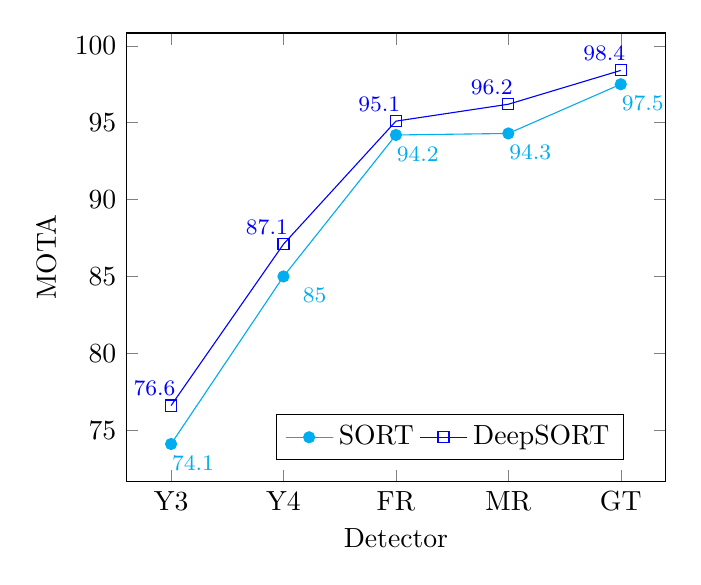
\begin{tikzpicture}
	\label{fig:pgf_mota}
	\begin{axis}[
		symbolic x coords={Y3,Y4,FR,MR,GT},
		xlabel=Detector,
		ylabel=MOTA,
		legend style={at={(0.6,0.15)},
			anchor=north,legend columns=-1},
		]
		\addplot [cyan,mark=*, nodes near coords,every node near coord/.append style={xshift=19pt,yshift=-7pt,anchor=east,font=\footnotesize},]
		coordinates {(Y3,74.1) (Y4,85)
			(FR,94.2) (MR,94.3) (GT,97.5)};
		\addplot [blue,mark=square,nodes near coords,every node near coord/.append style={xshift=-6pt, font=\footnotesize}]
		coordinates {(Y3,76.6) (Y4,87.1)
			(FR,95.1) (MR,96.2) (GT,98.4)};
		\legend{SORT,DeepSORT}
	\end{axis}
\end{tikzpicture}}
\resizebox{0.5\textwidth}{!}{%
	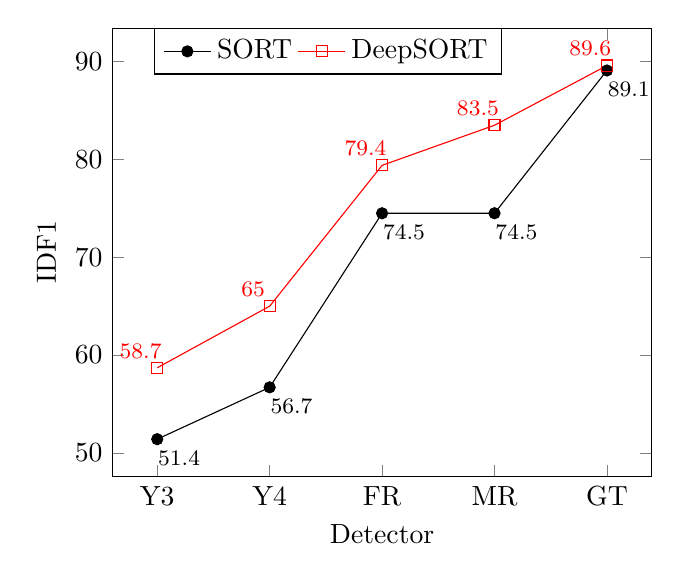
\begin{tikzpicture}
		\label{fig:pgf_idf1}
		\begin{axis}[
			symbolic x coords={Y3,Y4,FR,MR,GT},
			xlabel=Detector,
			ylabel=IDF1,
			legend style={at={(0.4,1.0)},
				anchor=north,legend columns=-1},
			]
			\addplot [mark=*, nodes near coords,every node near coord/.append style={xshift=19pt,yshift=-7pt,anchor=east,font=\footnotesize},]
			coordinates {(Y3,51.4) (Y4,56.7)
				(FR,74.5) (MR,74.5) (GT,89.1)};
			\addplot [red,mark=square,nodes near coords,every node near coord/.append style={xshift=-6pt, font=\footnotesize}]
			coordinates {(Y3,58.7) (Y4,65)
				(FR,79.4) (MR,83.5) (GT,89.6)};
			\legend{SORT,DeepSORT}
		\end{axis}
	\end{tikzpicture}
}
\caption{Overall MOTA and IDF1 metric on Micand32E.}
\end{figure}
\subsection{Impact of detection method over tracking result}
In the sub-section \ref{subsec:det_res}, the accuracy of the Yolo family models and RCNN family models are reported and we insists that in term of precision, the MaskRCNN and FastRCNN completely outperforms the Yolos. The impact of choosing detection tactic on the tracking performance is also shown clearly in Figure 4 1 and Figure 4 2. On the same tracking method, SORT, MOTA results of Yolov3, Yolov4, FasterRCNN, MaskRCNN and detection groundtruth are respectively 74,1\%, 85\%, 94,2\%, 94,3\% and 97,5\%. Also it’s remarkable that the number of FN decreases, 3176 for Y3DS, 1581 for Y4DS, 282 for FDS, 184 for MDS and 82 for GDS. After researching theory and evaluating experiments, it’s quit intuitive but reasonable to conclude that the better detection method is, the higher tracking quality is.
\subsection{Complexity of 4 types of patients's actions}
The diversity and complexity of 4 type of patient’s actions are analyzed via metrics in Table \ref{tab:long_gds}, the highest results achieved in this experiment. In term of MOTA metric, the GDS obtains best performance on the action type 6, with 2 sequences:  GH010373\_6\_3150\_4744 99,7\% and GH010358\_6\_10208\_11900 99\%. On the contrary, the MOTA for GH010358\_8\_8000\_5447 is 96,1\% with GDS.
On the other hand, the sequence’s volume also has impacts on the tracking qualities. All videos in Micand32S are short-term and the results of all the 11 approaches is almost perfect on this datasets. But in Micand32E, the sequences is long and then many weaknesses of tracking algorithms appear, it’s visible via the metrics like IDP and IDR. However, on both datasets, almost approaches can still track hands well, this is shown by metric GT and MT in Table \ref{tab:long_overall}.
\subsection{Challenging cases}
According to my personal coding experience through this thesis, multiple object tracking is quit difficult to debug errors. The evaluation process is not reversible, when the results are available, the metrics can be calculated, but by just looking at the metrics, it’s hard to know where the errors occur, we can only visualize the result through visible video to find the bug. In this way, I find some challenging cases in some sequences that make almost of 11 approaches yield tracking errors. Some typical cases are enumerated as follow:
\begin{itemize}
	\item When hands are occluded by other obstacles. Trackers lost information about these hands due to the detector naturally can't find those hands. In figure \ref{fig:occluded}, in the first, from frame \(200^{th}\) to \(250^{th}\), SORT are tracing the right hand with ID 1. In the second row, from frame \(256^{th}\) to frame \(261^{th}\), an experimental equipment - a "toy house", has significantly obscured the right hand part. This makes FasterRCNN can't recognize that hand (false positive), and therefore, SORT lost that hand's trajectory. Until frame \(267^{th}\), the hand goes out of the equipment and can be seen clearly. In the third row, FasterRCNN can predict again that right hand, but the shape of the hand seems to be too different for the first row, and of course, SORT initialize a new ID 7 for the hand. A remarkable point in this case is that, with the same condition, the left hand isn't overlapped by the "toy house", so both FaterRCNN and SORT worked perfectly, it keeps the ID 4 for the left hand through all the time.
	\item When a hand moves rapidly so that the cameras can’t catch, this make the motion blur phenomenon occur. As a result, detectors fail to predict the existence of the hand. For example, in figure \ref{fig:blur}, in the frame \(119^{th}\), the trackers are tracing the ID 1, but in the following frames from \(120^{th}\) to \(142^{th}\) Yolov3 can't predict the hand's existence (false positive), until the frame \(143^{th}\) it find that hand again but at this time the tracker can't retrieve the hand's identity, it initialize a new ID 2 for the hand.
	\item When the shape of the hand changes heavily. Intuitively, the deep appearance descriptor doesn't work in this case, it simply can't recognize that these different shapes belong to a same id. Consequently, a new ID is initialized and then ID switches occur. In figure \ref{fig:shape}, DeepSORT works stability in frames \(1582^{th}, 1592^{th}, 1602^{th}, 1612^{th}, 1622^{th}\) with the hand ID 5. But in frame \(1630^{th}\), the shape of the right hand changes heavily, DeepSORT initialize a new ID 7 for that hand. Figure \ref{fig:occluded} also proves this: the shape of the right hand in the first row and the third row is too different, and certainly, SORT assign 2 identities for just 1 hand.
	\item The ambiguous  definition of the "hand" causes difficulty. Detection model is training on both GTEA family ("hand" includes wrist, arm) and EgoHand ("hand" just includes hand) so the during inference stage, the detector may be quite tough. In figure \ref{fig:definition}, FasterRCNN and SORT keep the left hand awesomely through 283 frames for \(1123^{th}\) to \(1406^{th}\) with ID 22, presented in the first row. Suddenly, in frame \(1407^{th}\), FasterRCNN predicts this left hand including the wrist. This makes SORT assign a new ID 24 for that hand as show in the second row. This issue is reported and will be discussed in the future work in the section \ref{sec:futurework}.
	\item When the hands disappear from the camera’s view and return after a long time, this makes the tracker "forget" that instance.
\end{itemize}
\begin{figure*}[ht!]
	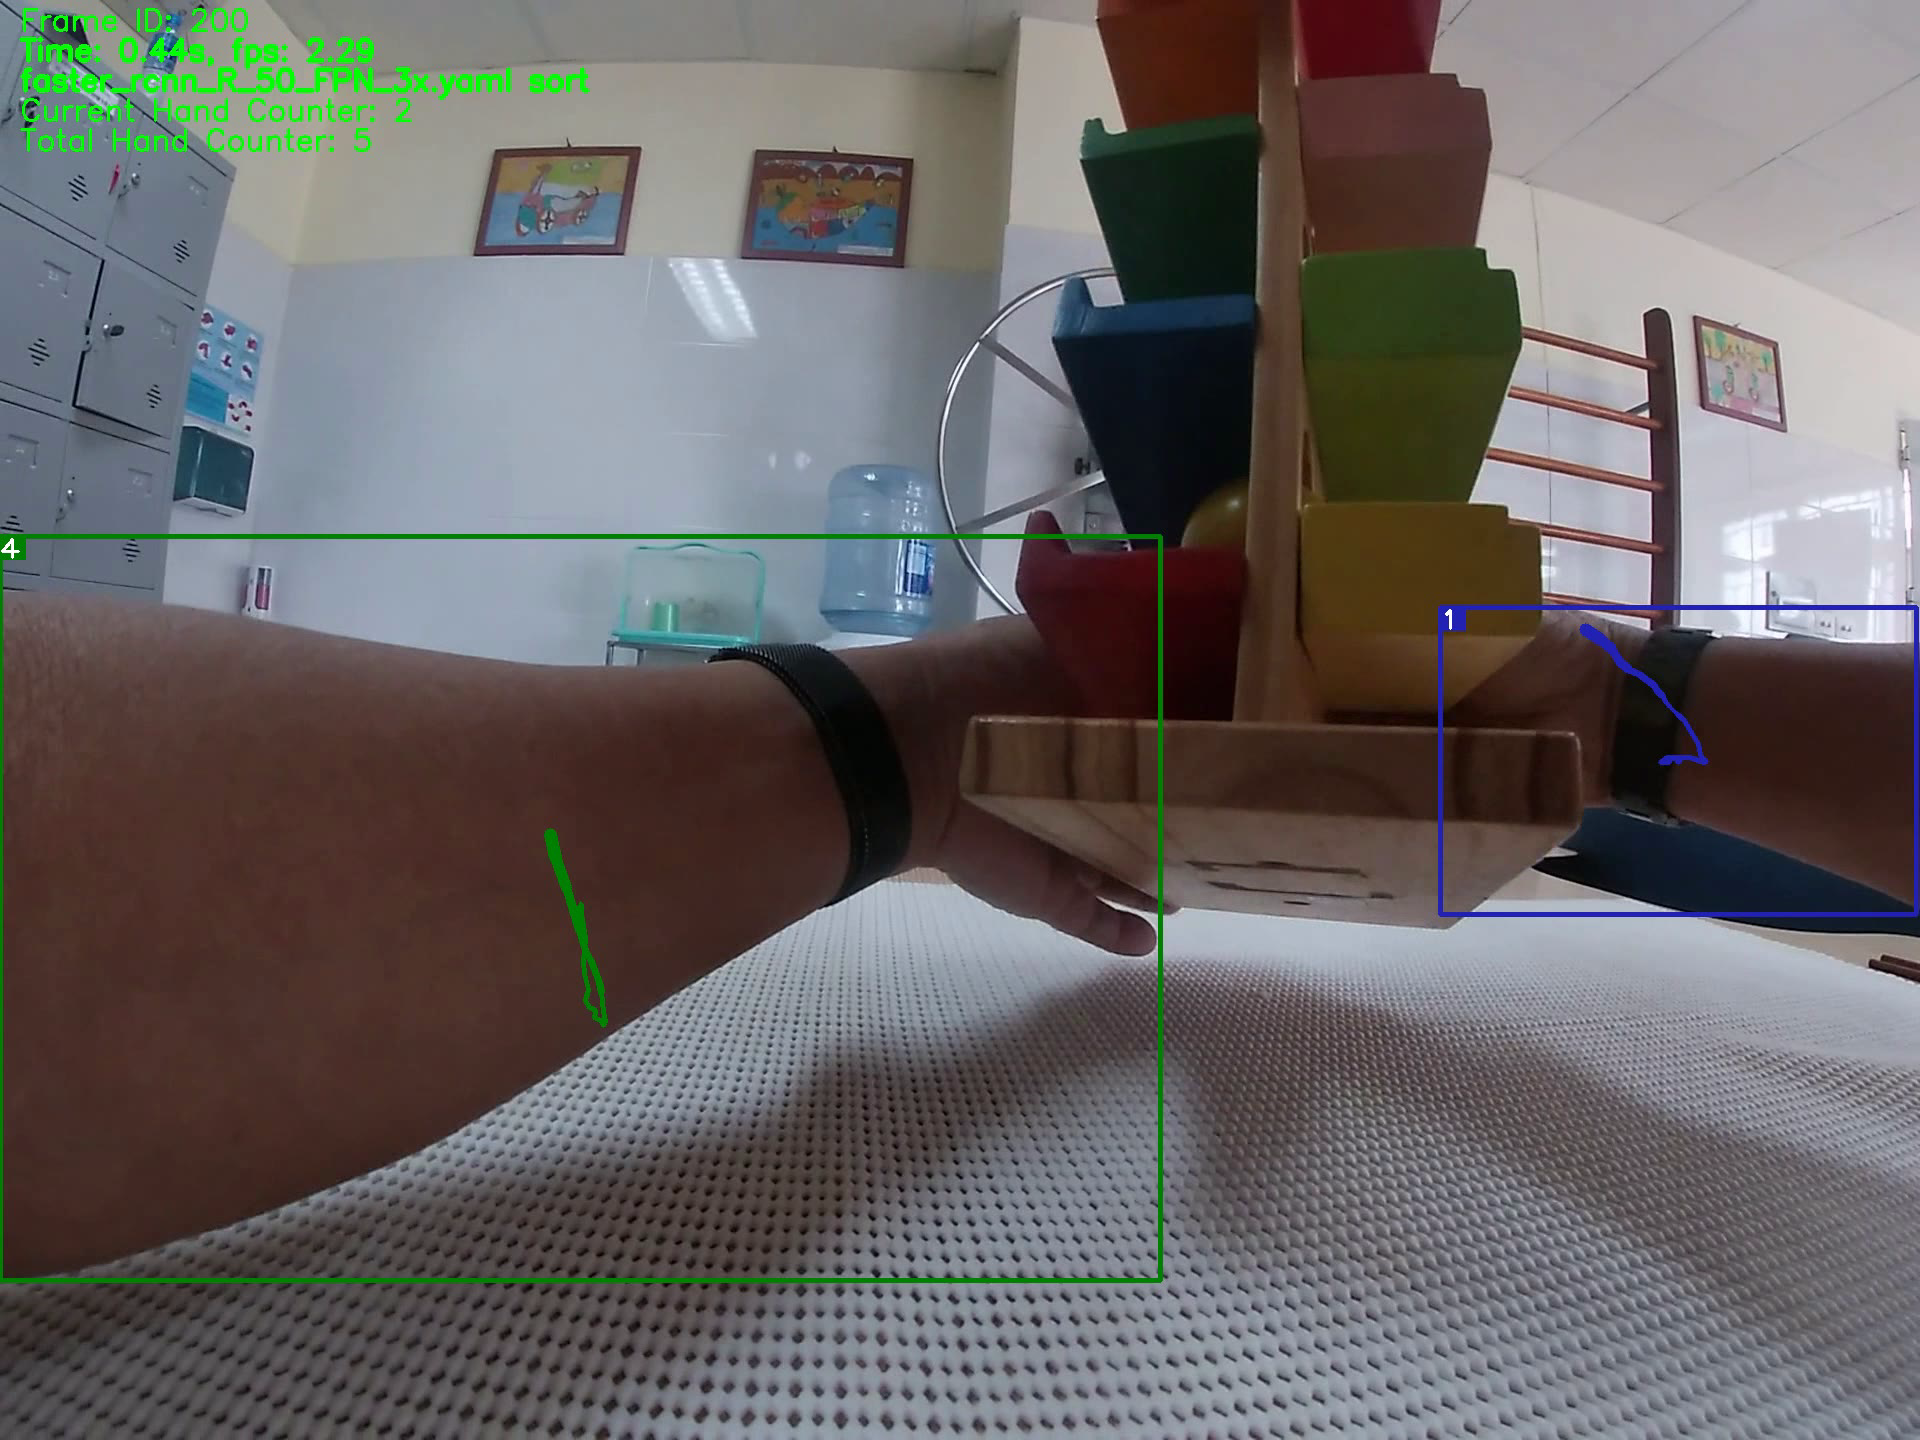
\includegraphics[width=.16\textwidth]{Figs/Occluded/200.png}
	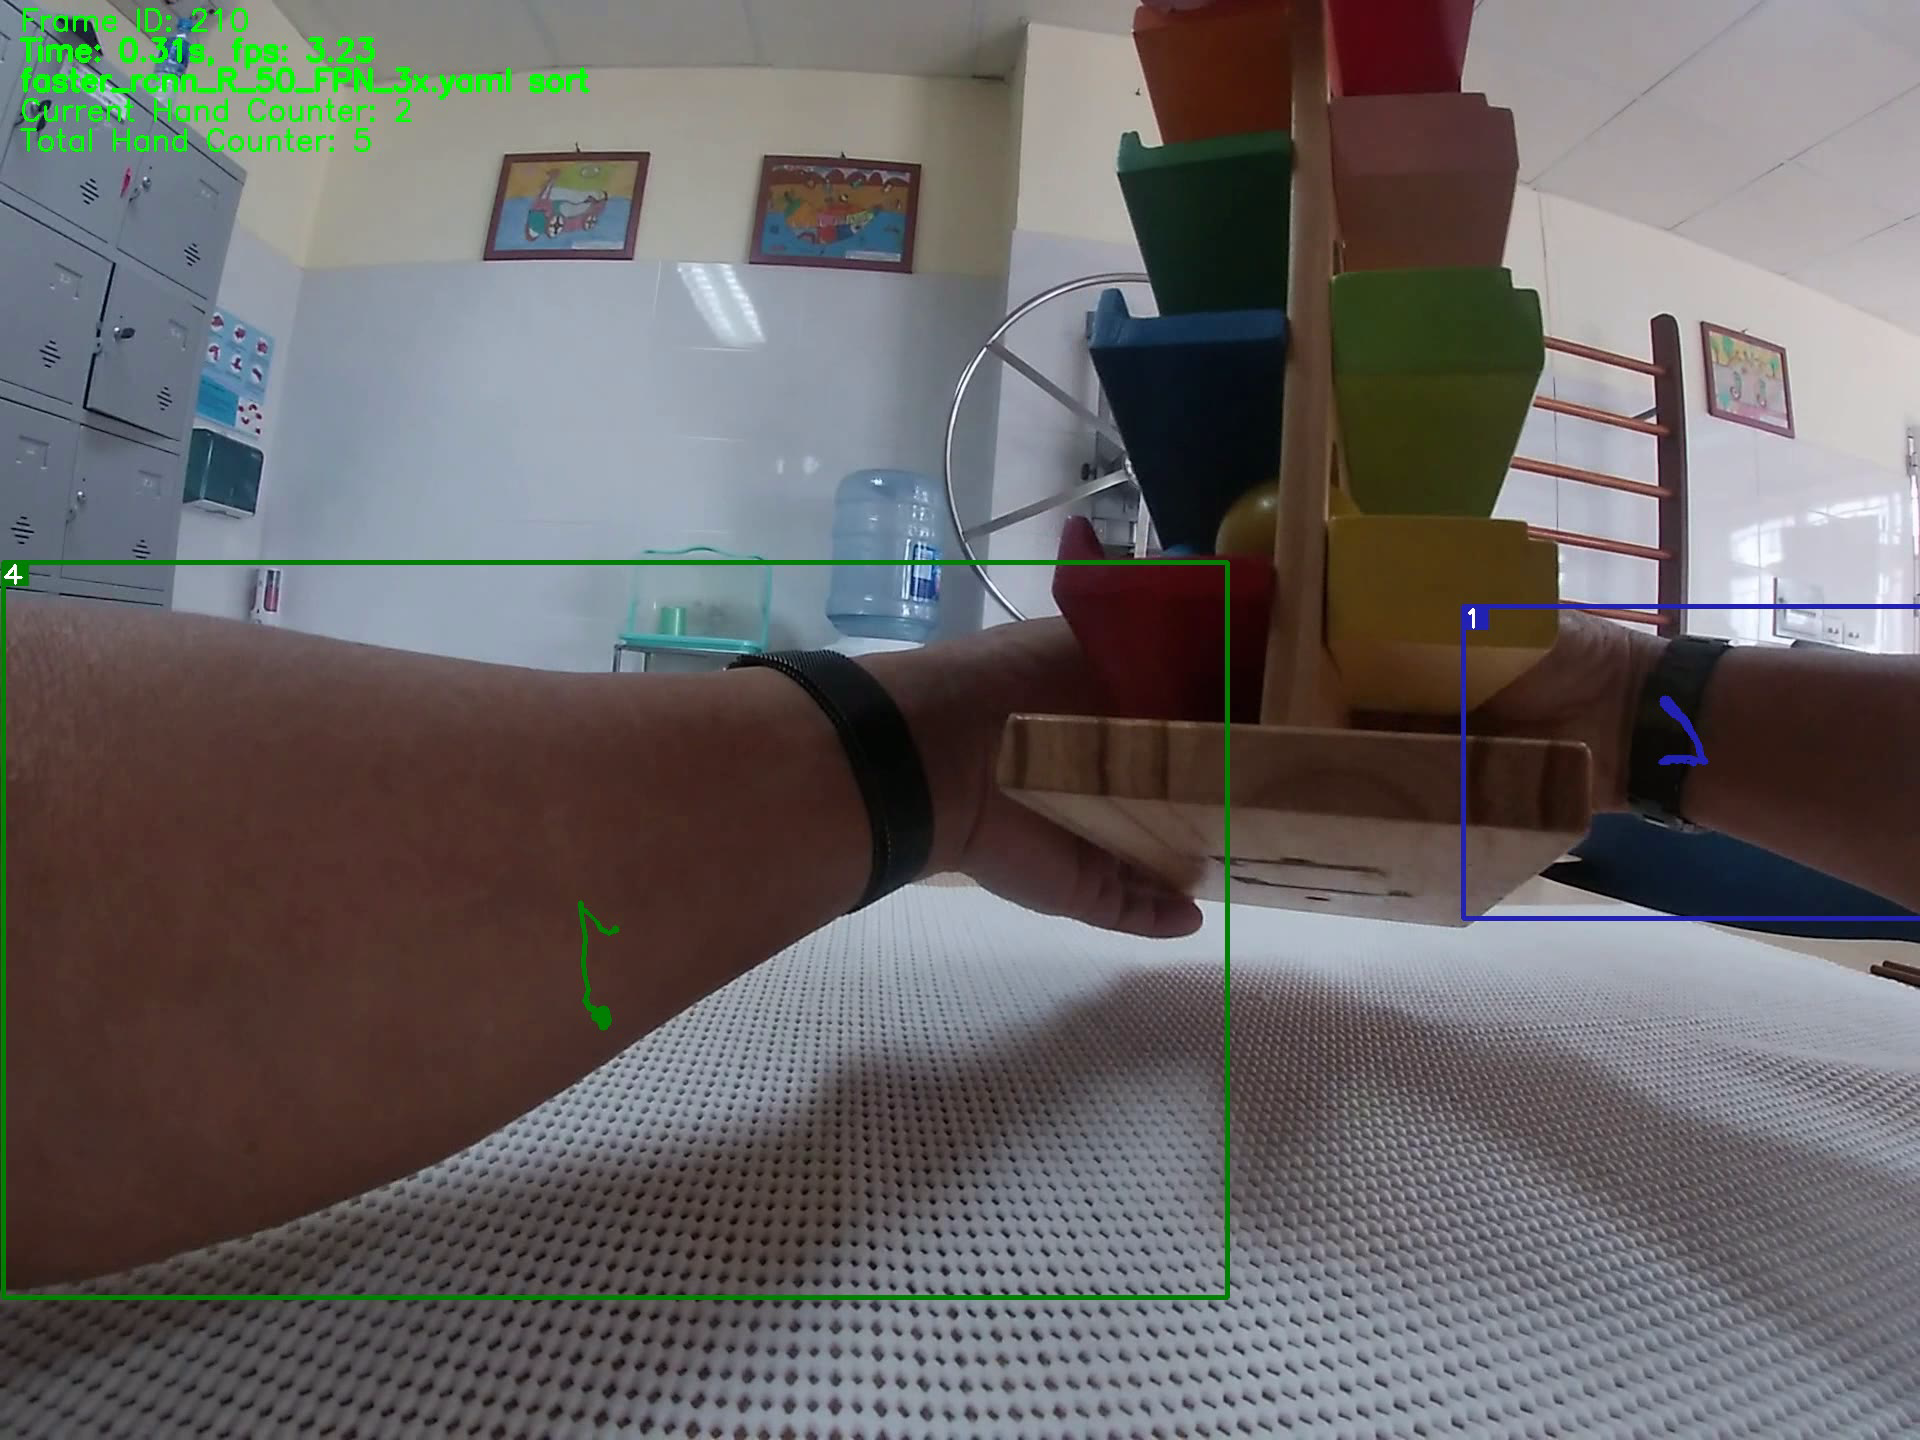
\includegraphics[width=.16\textwidth]{Figs/Occluded/210.png}	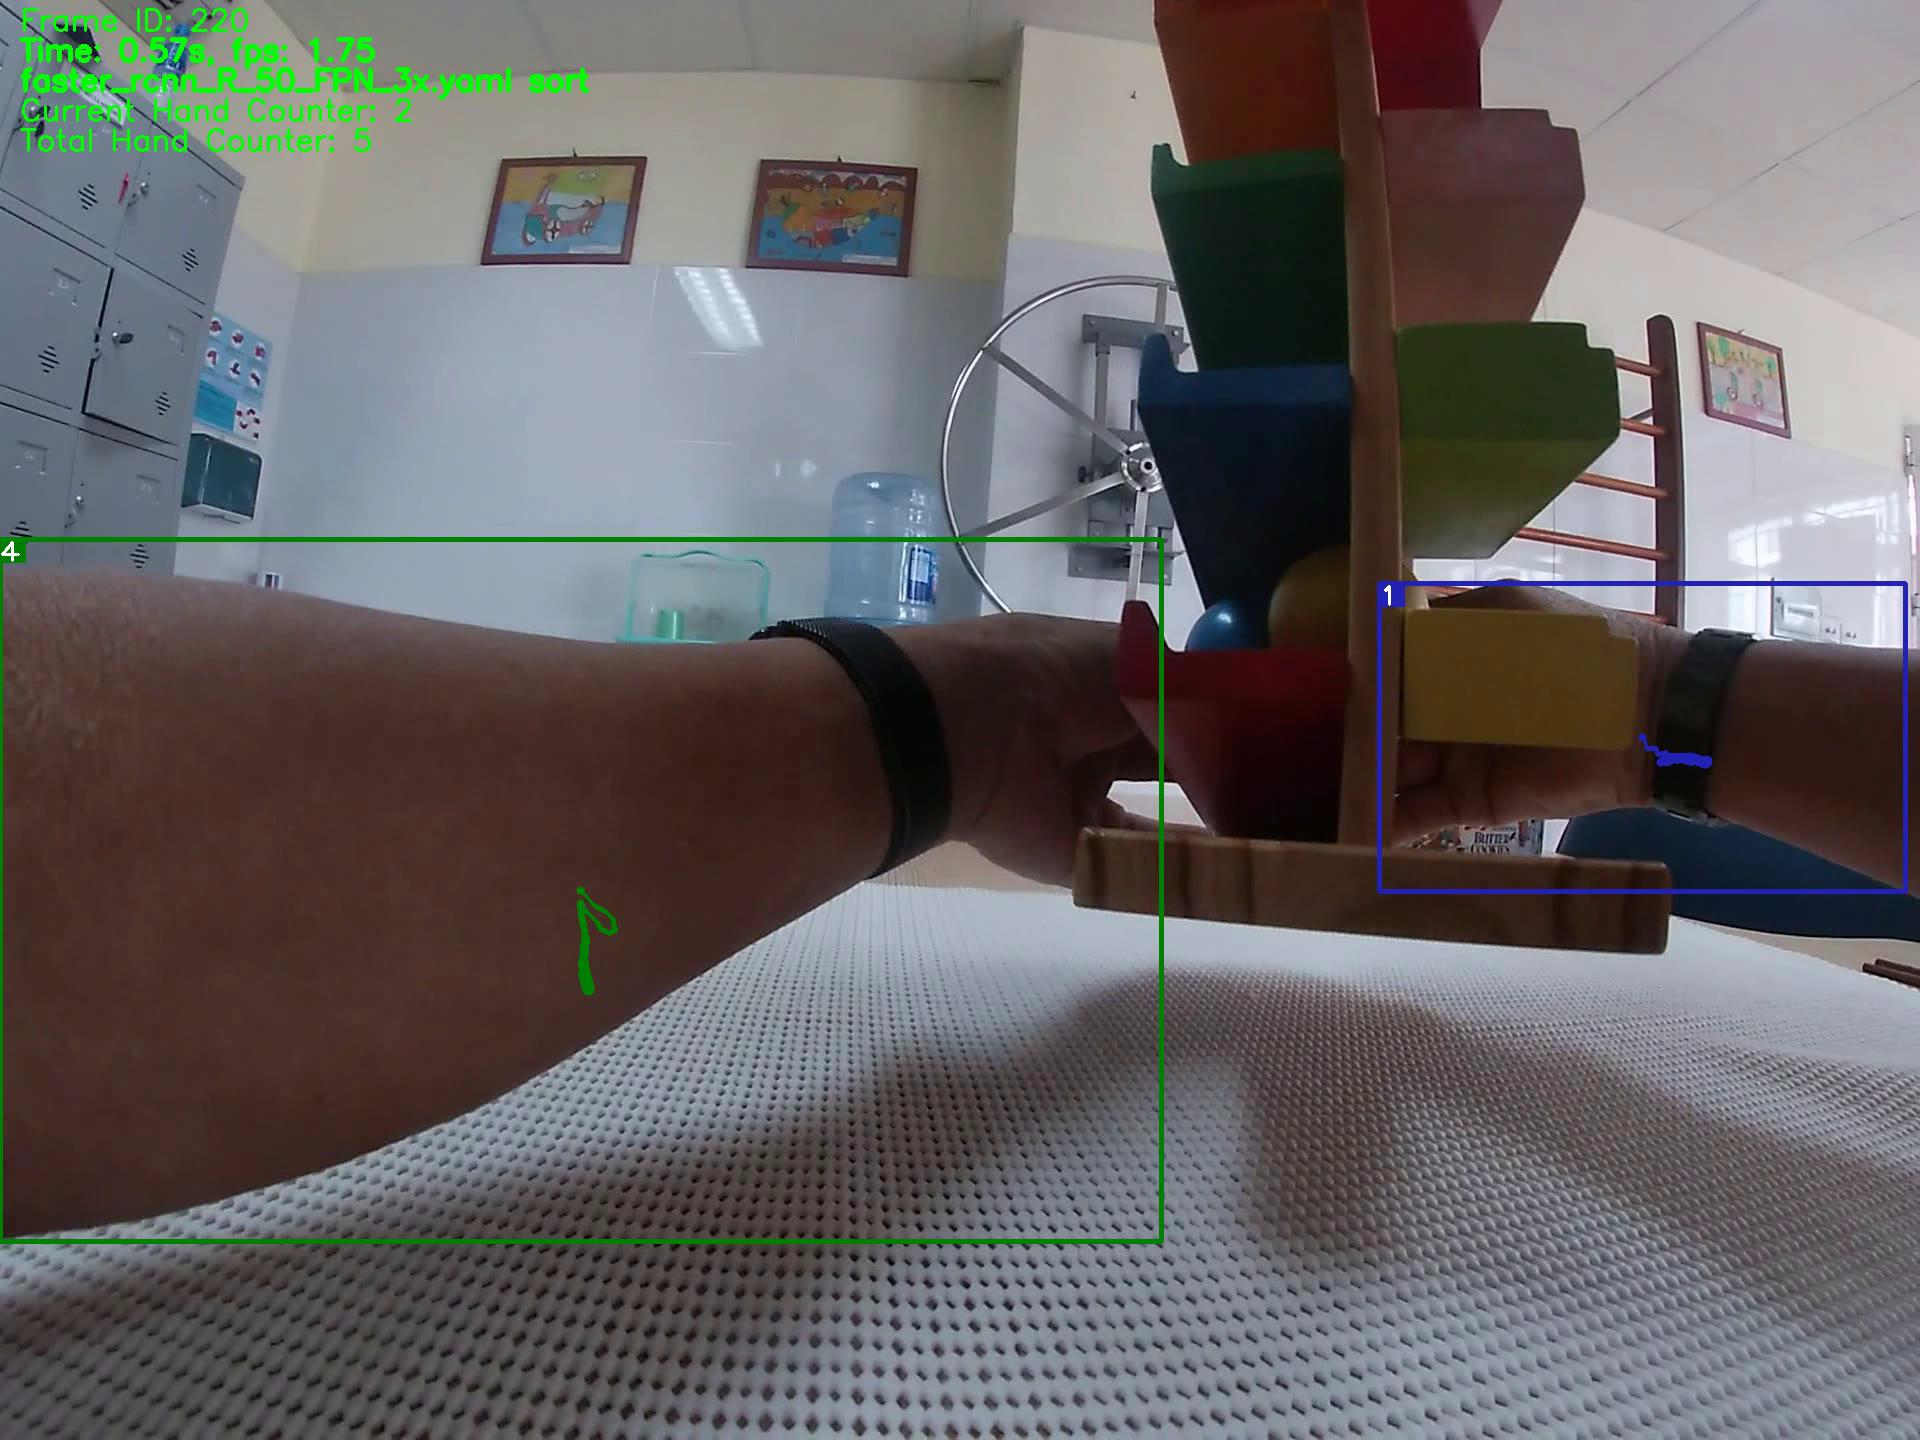
\includegraphics[width=.16\textwidth]{Figs/Occluded/220.png}
	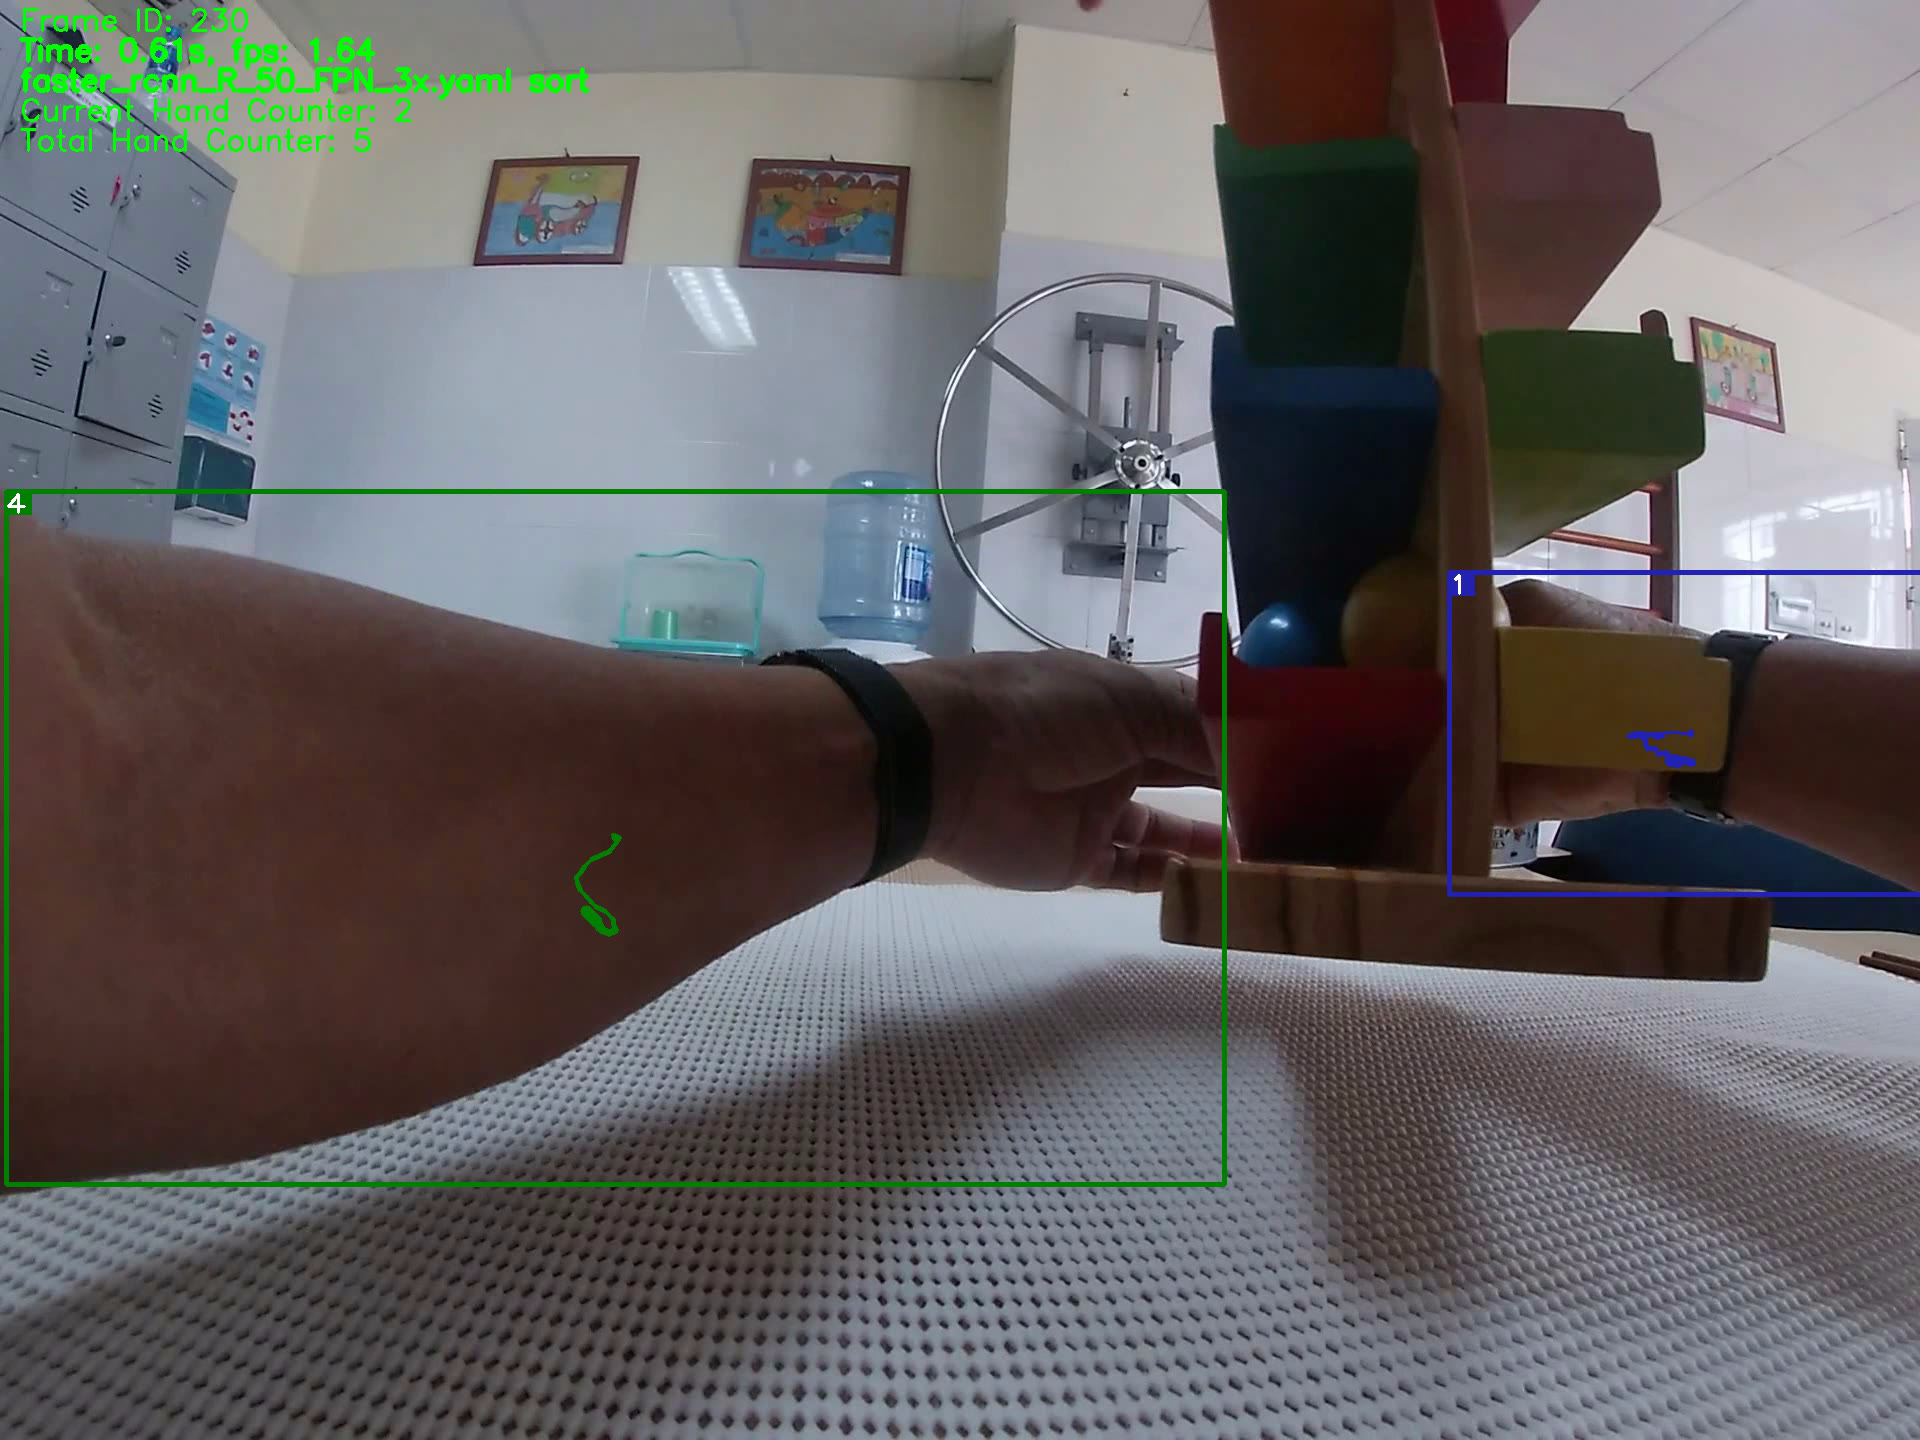
\includegraphics[width=.16\textwidth]{Figs/Occluded/230.png}	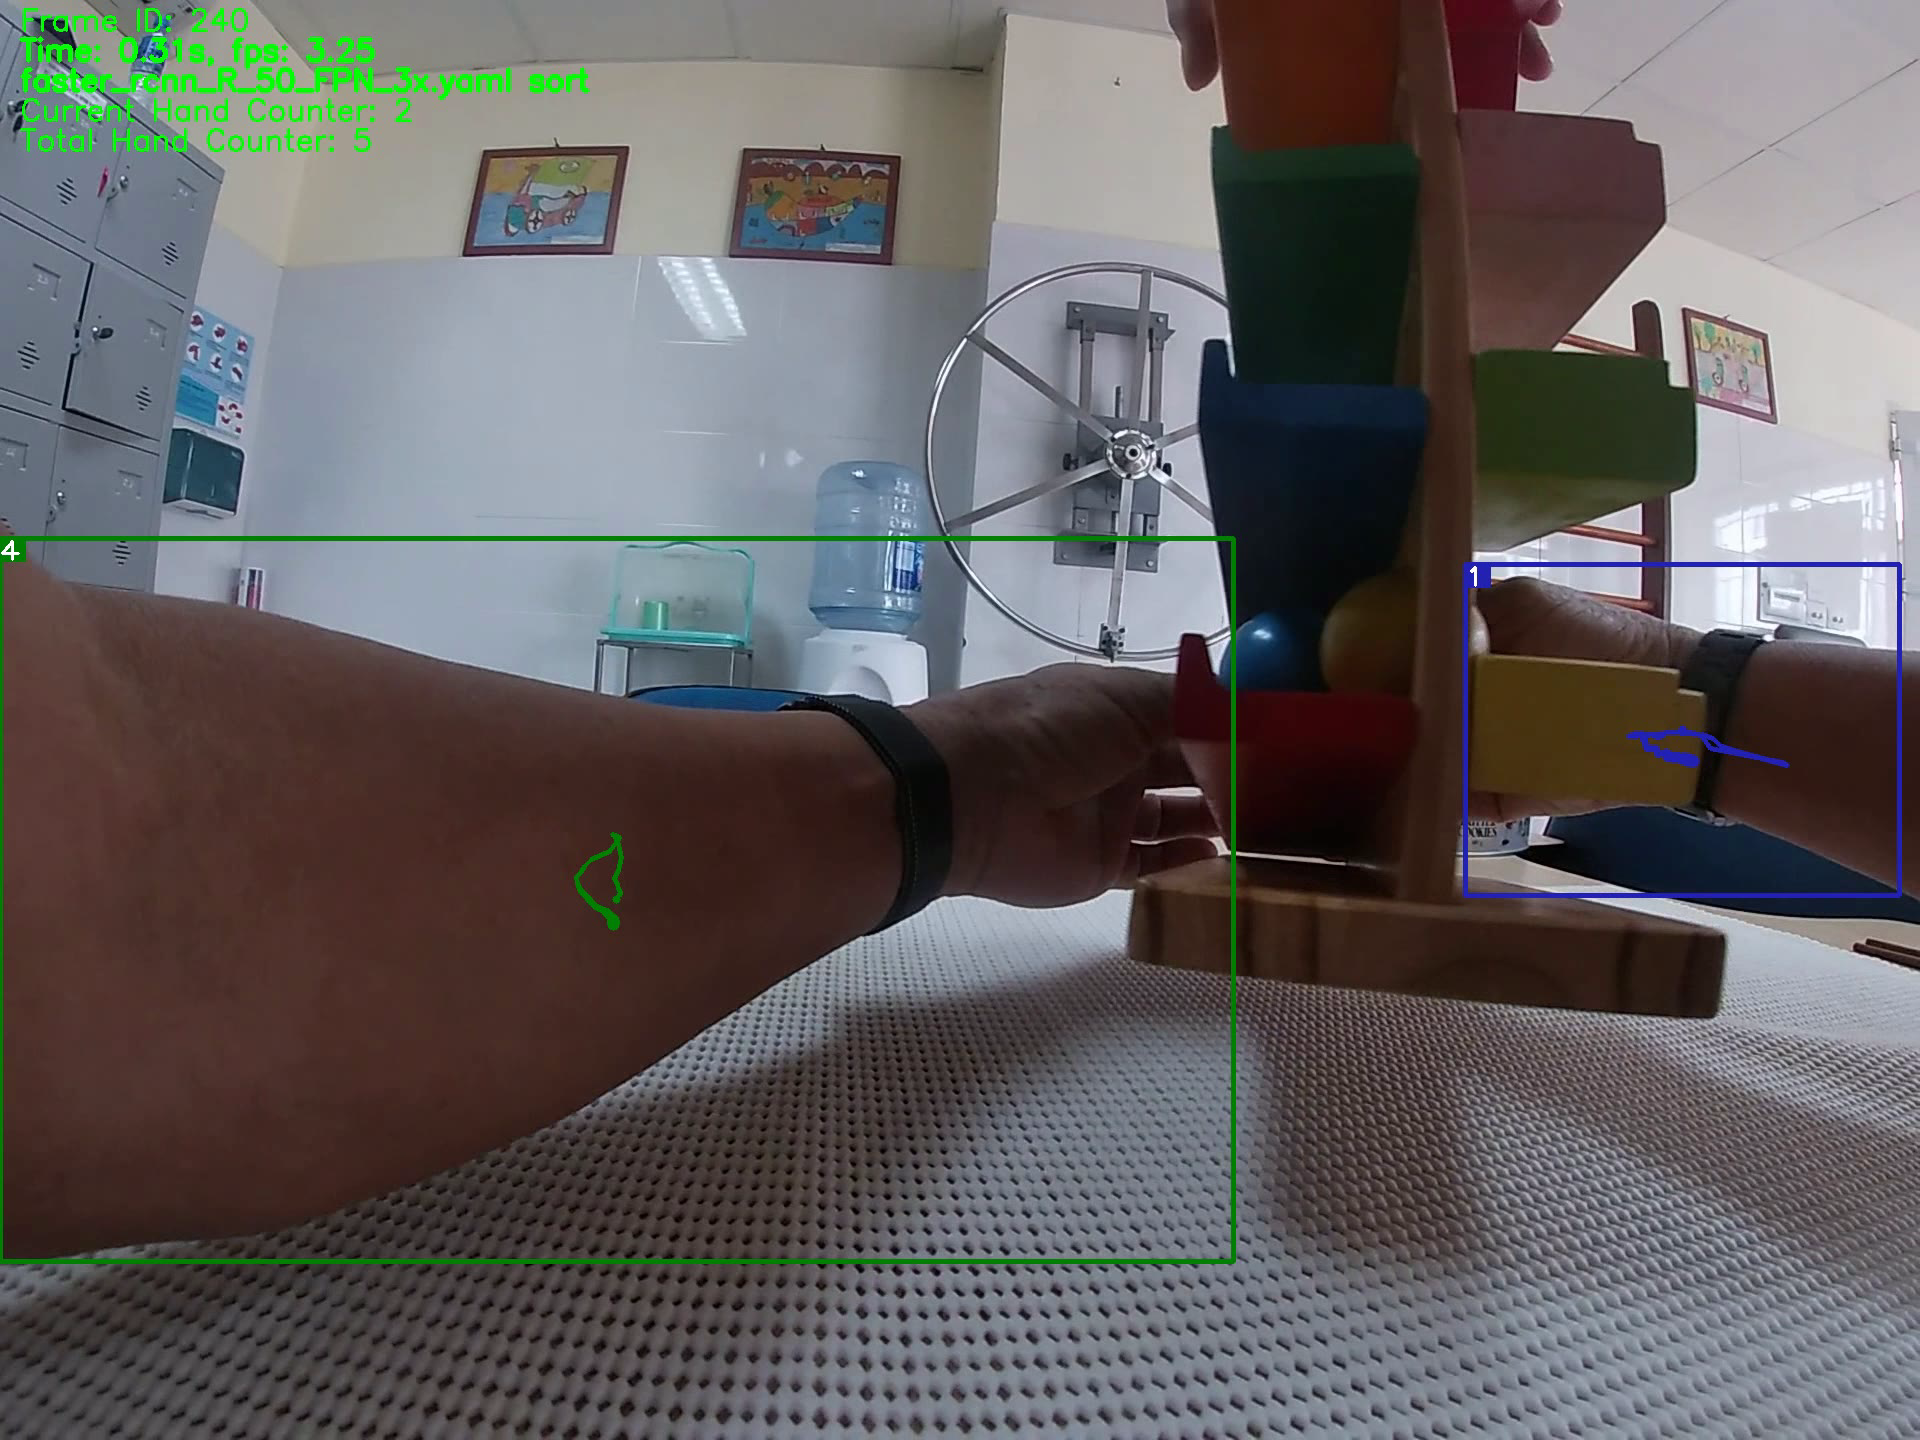
\includegraphics[width=.16\textwidth]{Figs/Occluded/240.png}
	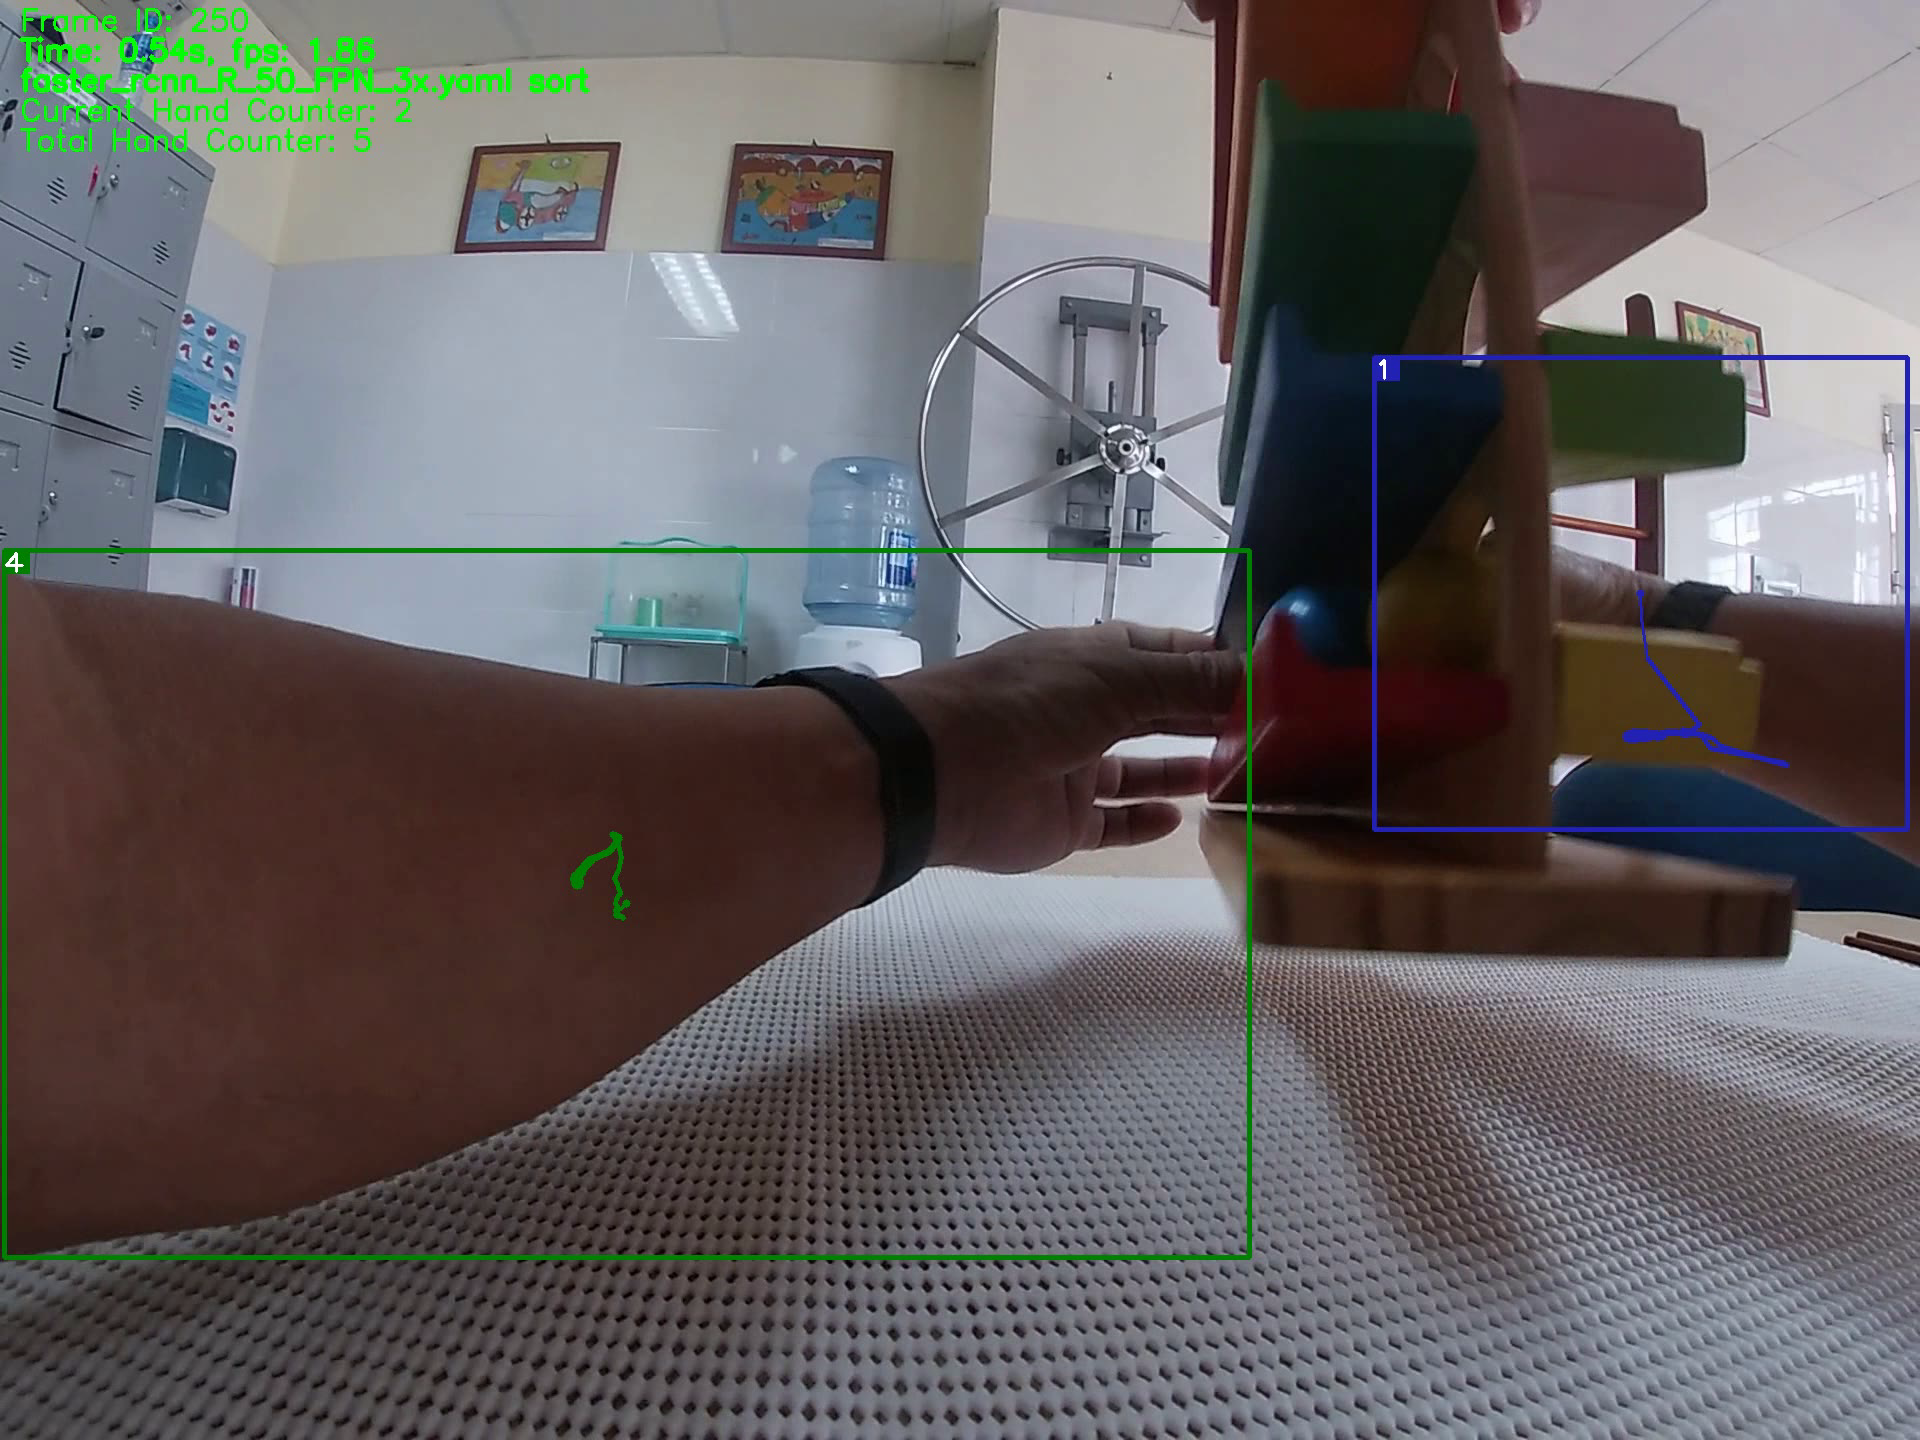
\includegraphics[width=.16\textwidth]{Figs/Occluded/250.png}
	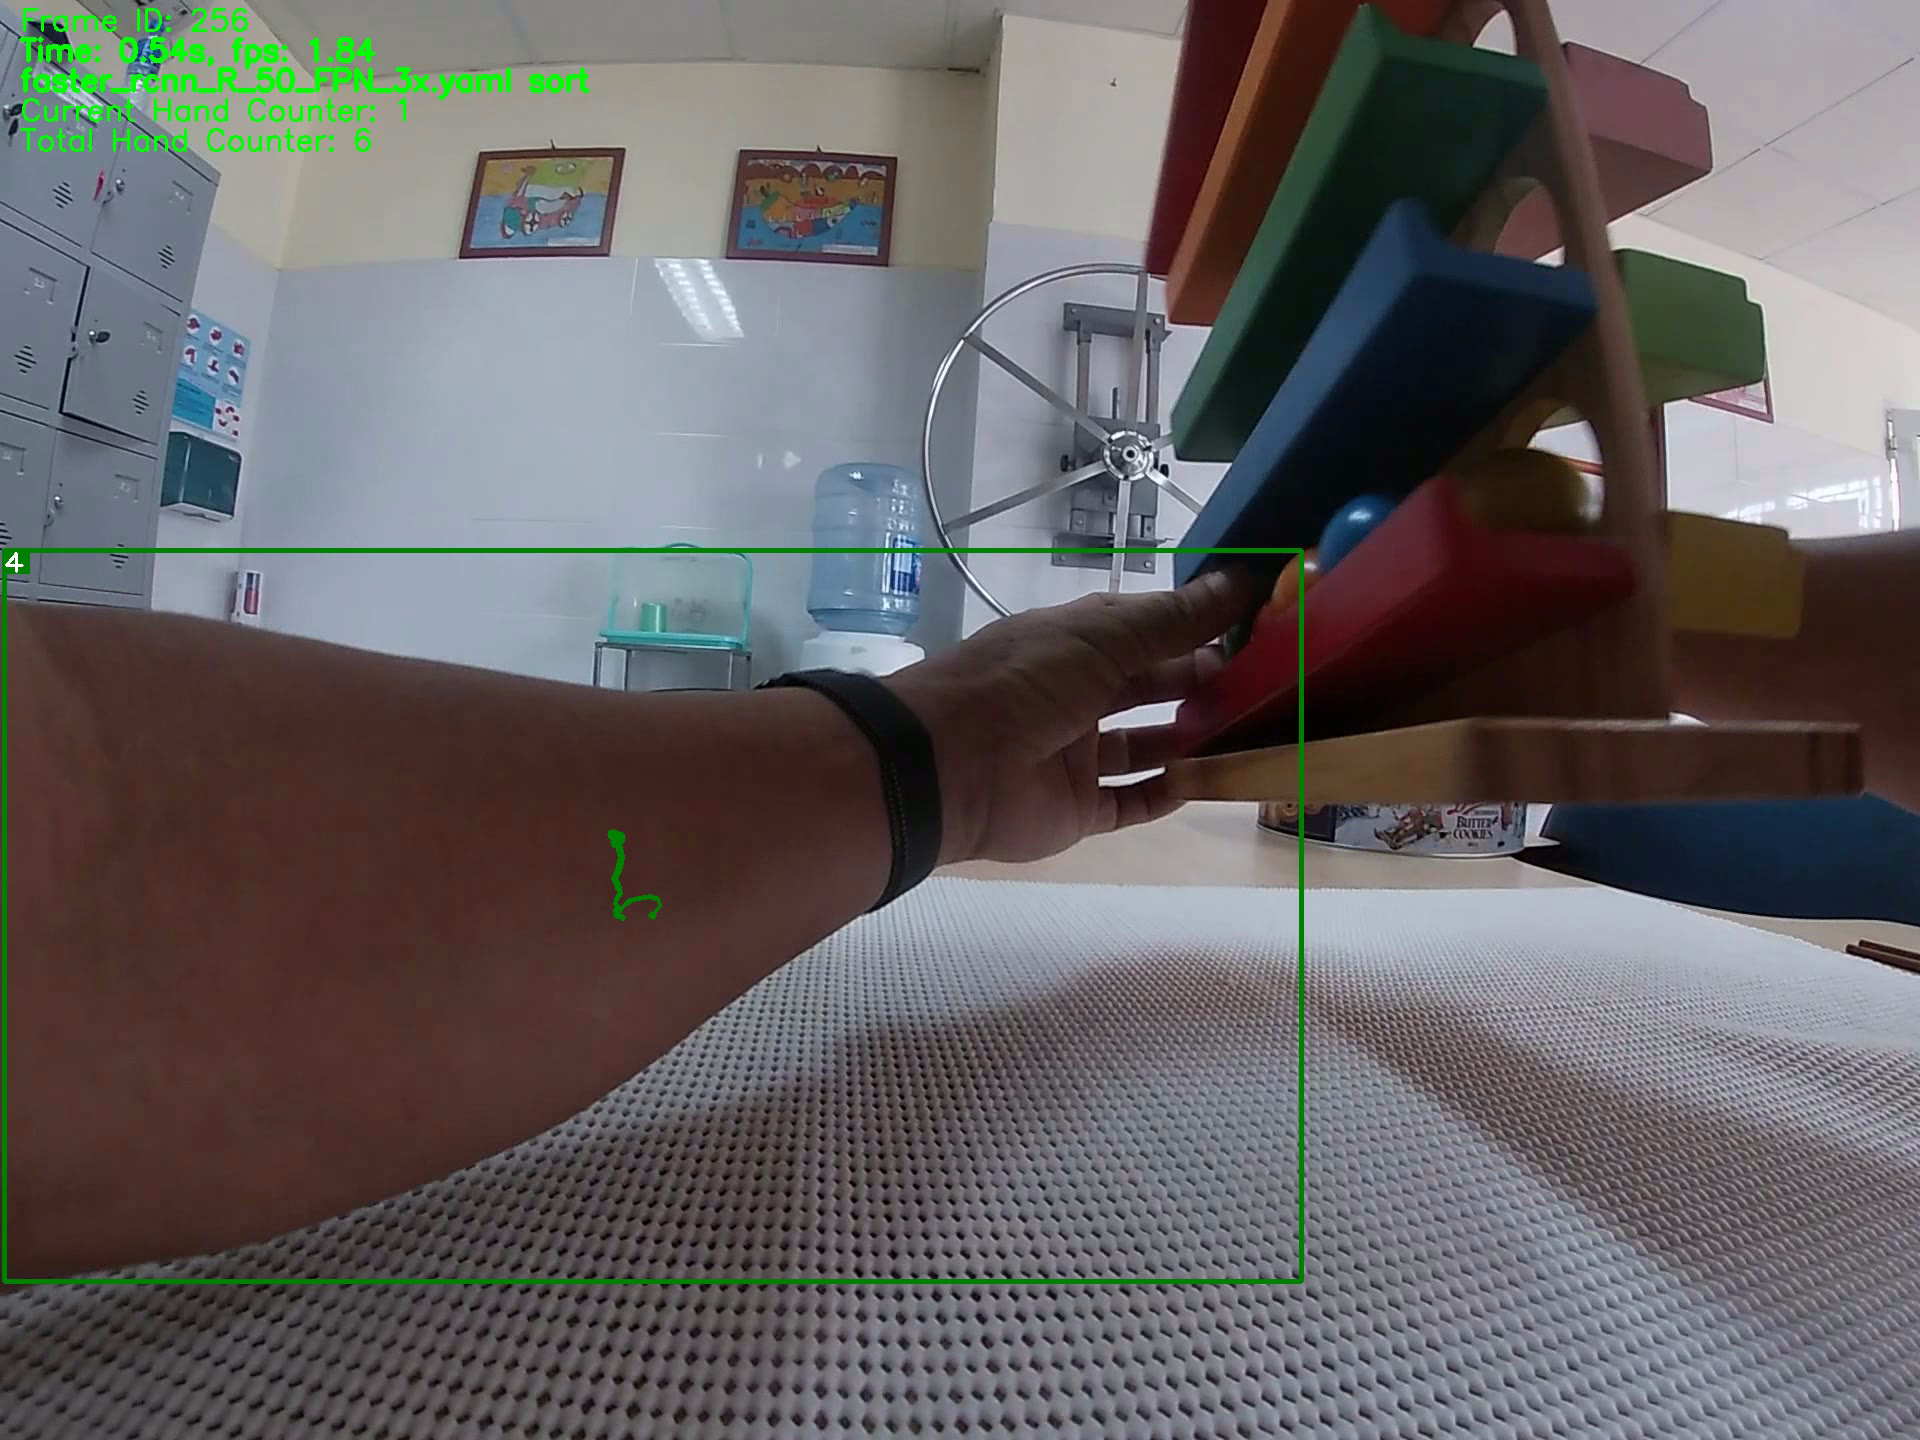
\includegraphics[width=.16\textwidth]{Figs/Occluded/256.png}
	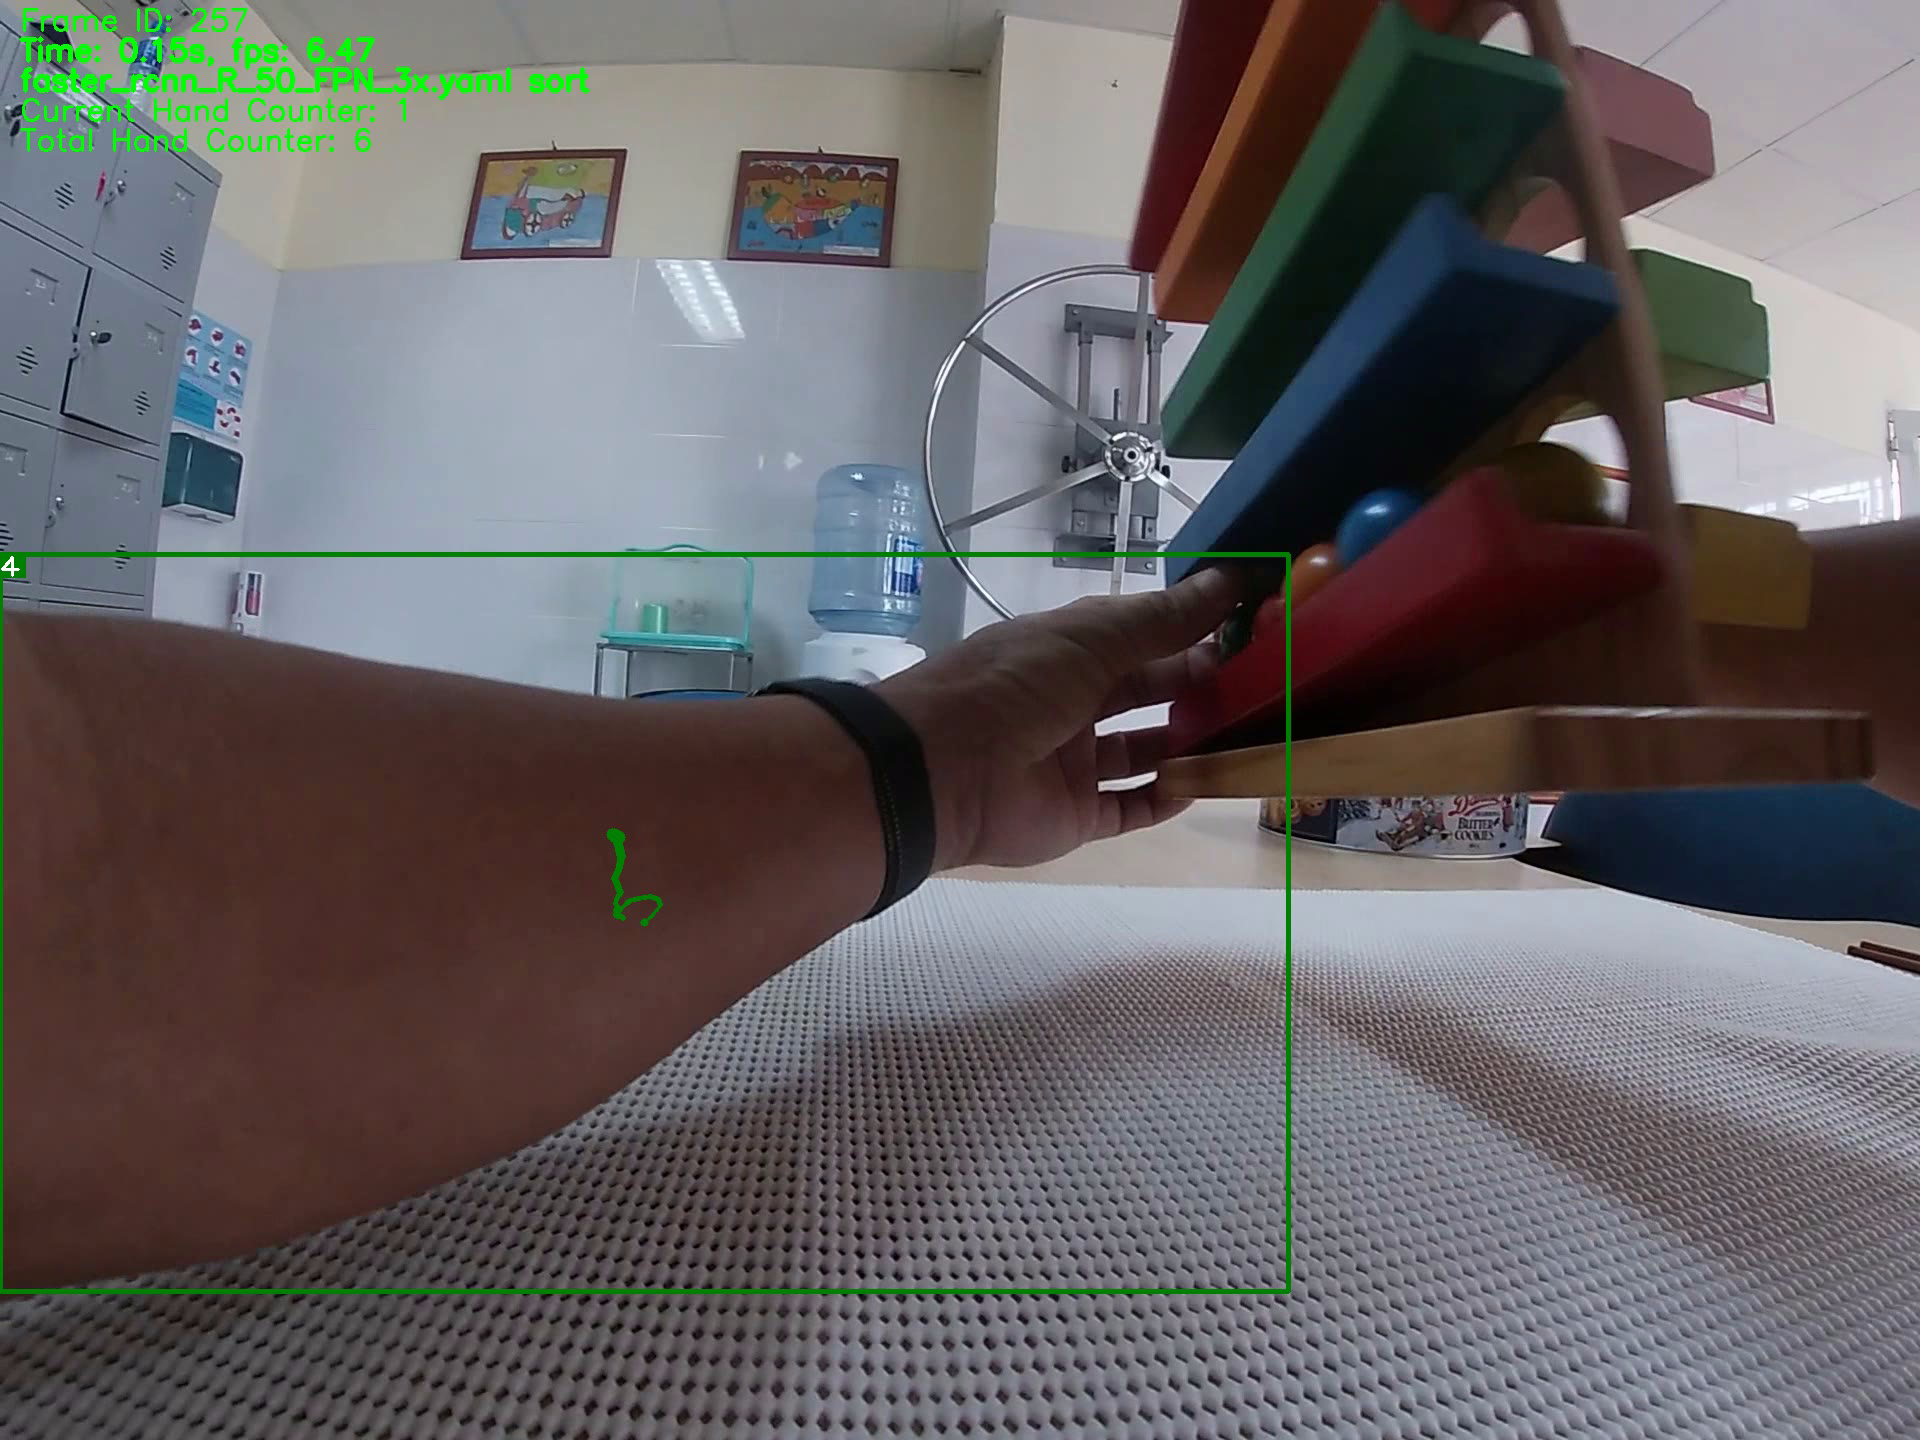
\includegraphics[width=.16\textwidth]{Figs/Occluded/257.png}	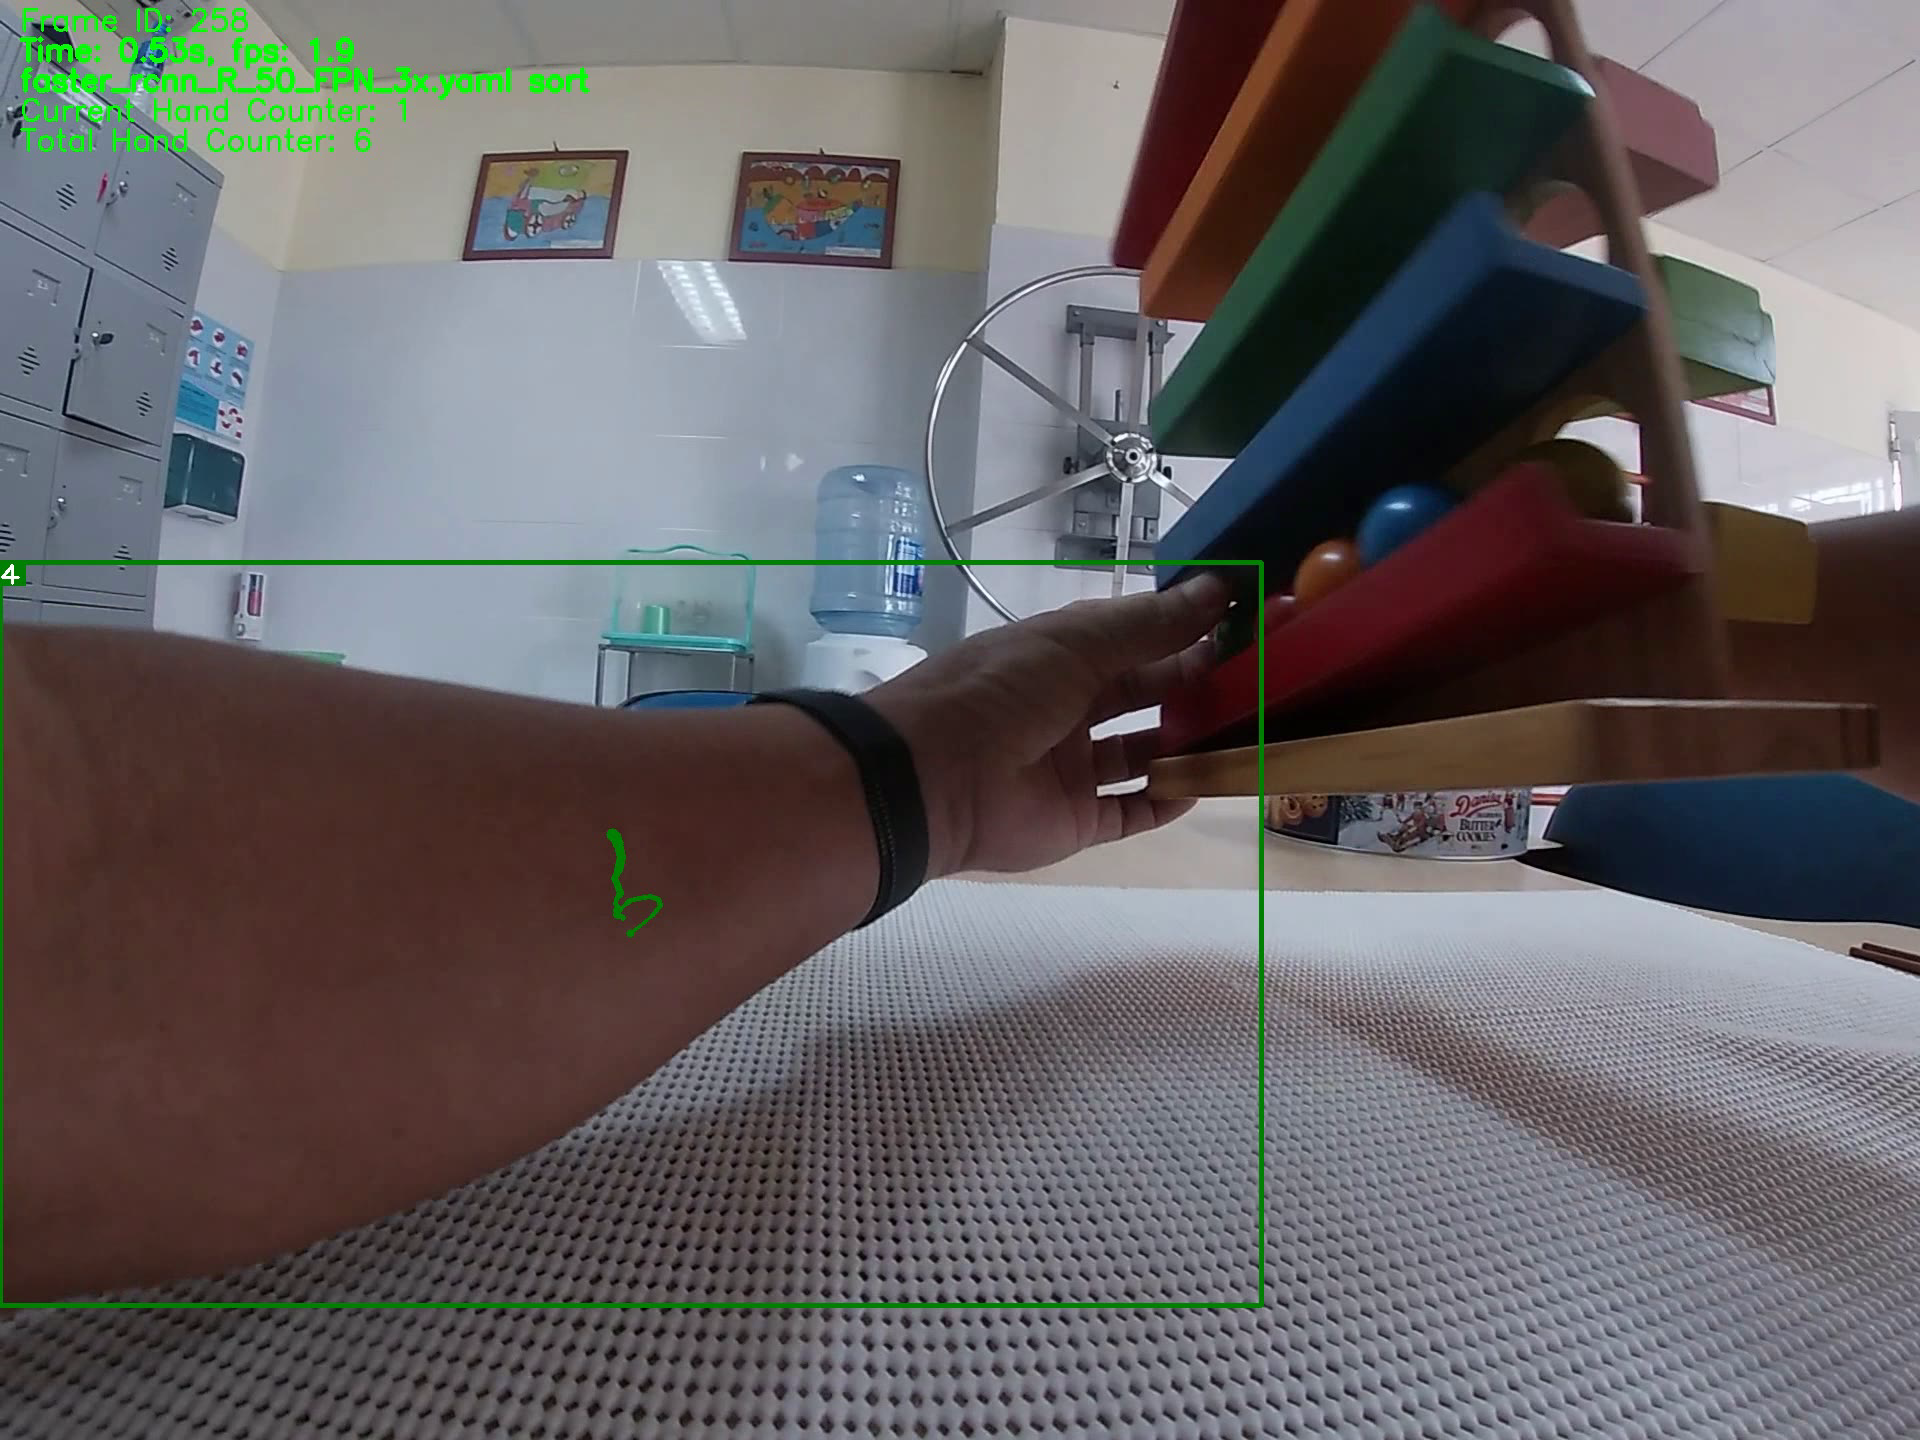
\includegraphics[width=.16\textwidth]{Figs/Occluded/258.png}
	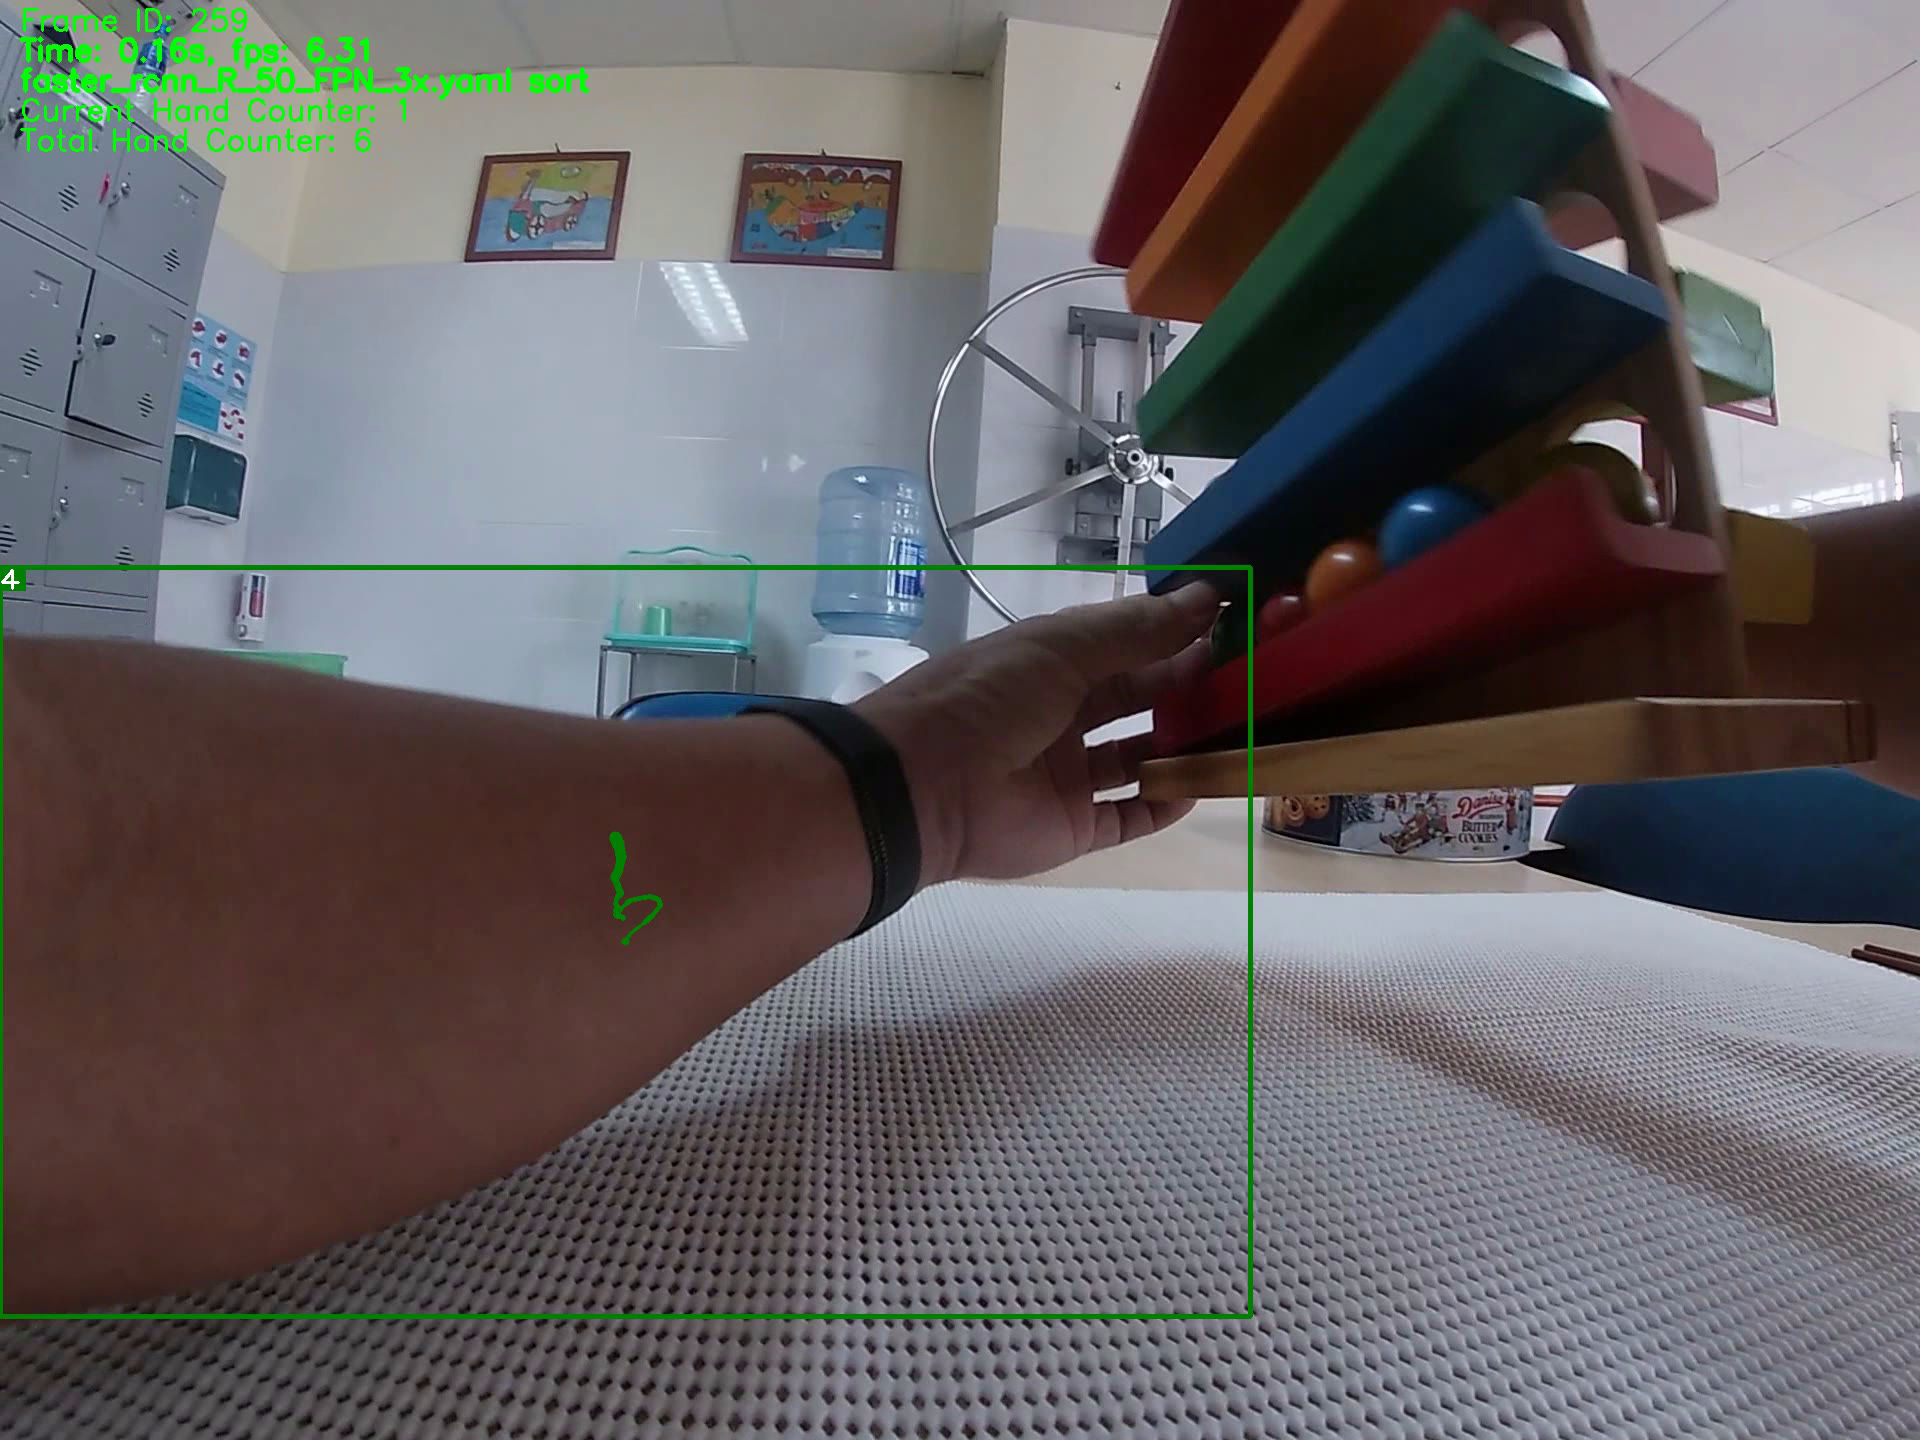
\includegraphics[width=.16\textwidth]{Figs/Occluded/259.png}	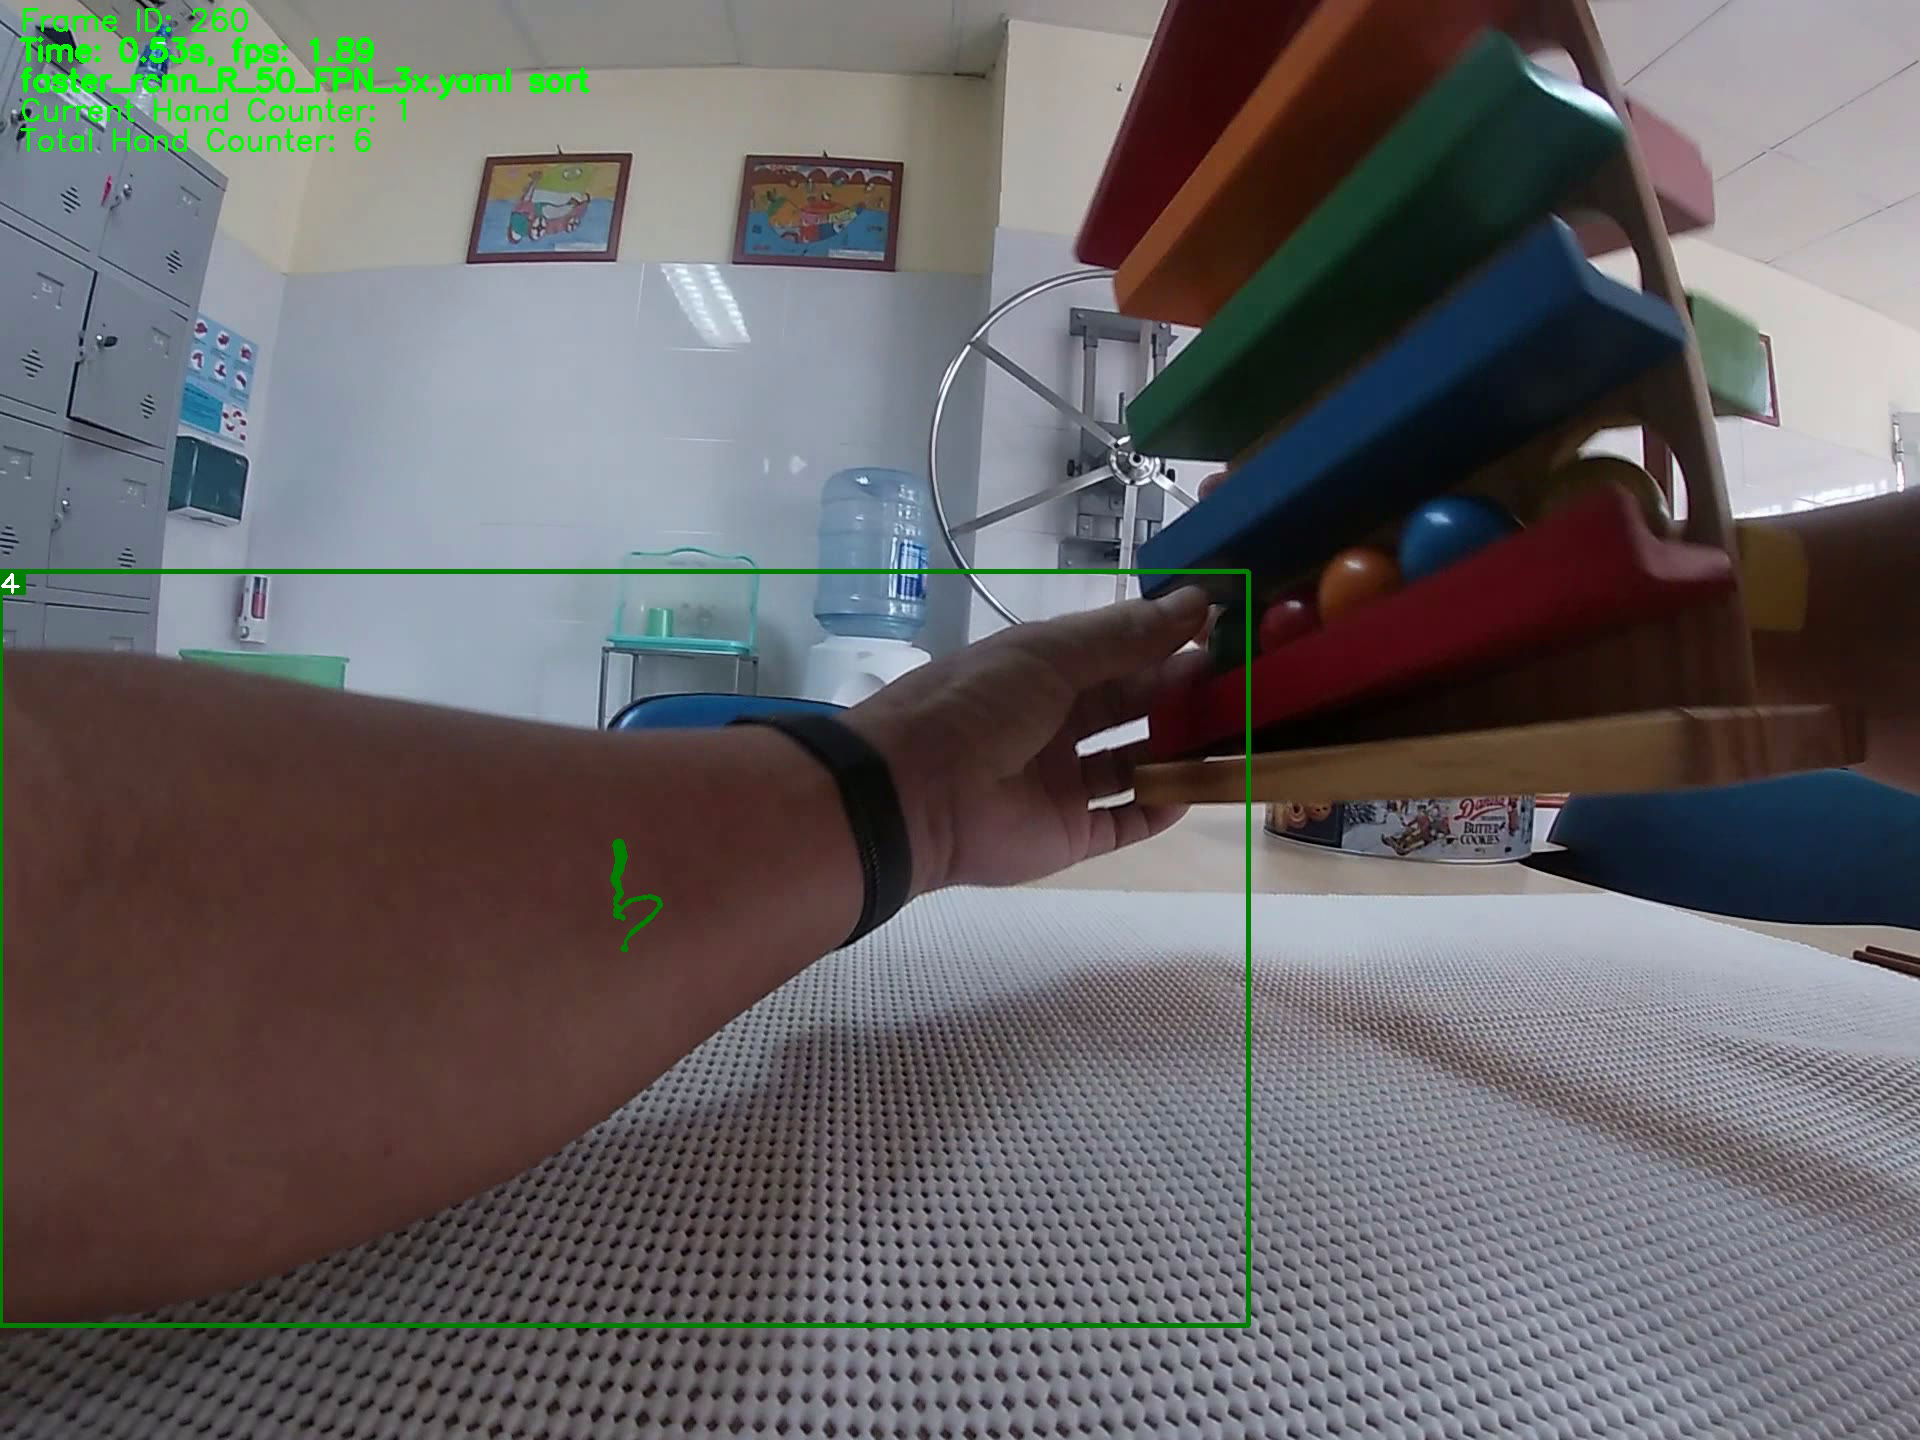
\includegraphics[width=.16\textwidth]{Figs/Occluded/260.png}
	\includegraphics[width=.16\textwidth]{Figs/Occluded/261.png}
	\includegraphics[width=.16\textwidth]{Figs/Occluded/267.png}
	\includegraphics[width=.16\textwidth]{Figs/Occluded/270.png}	\includegraphics[width=.16\textwidth]{Figs/Occluded/273.png}
	\includegraphics[width=.16\textwidth]{Figs/Occluded/276.png}	\includegraphics[width=.16\textwidth]{Figs/Occluded/279.png}
	\includegraphics[width=.16\textwidth]{Figs/Occluded/282.png}
	\caption{Illustration of hand occluded by an obstacle. Pay attention to the patient's right hand. Frames extracted from GH010373\_5\_1284\_2724 using FasterRCNN+SORT, ordered from left to right, up to down: (200, 210, 220, 230, 240, 250), (256, 257, 258, 259, 260, 261), (267, 270, 273, 276, 279, 282).}
	\label{fig:occluded}
\end{figure*}
\begin{figure*}[ht!]
	\includegraphics[width=.16\textwidth]{Figs/blur/119.png}
	\includegraphics[width=.16\textwidth]{Figs/blur/120.png}	\includegraphics[width=.16\textwidth]{Figs/blur/125.png}
	\includegraphics[width=.16\textwidth]{Figs/blur/131.png}	\includegraphics[width=.16\textwidth]{Figs/blur/137.png}
	\includegraphics[width=.16\textwidth]{Figs/blur/143.png}
	\caption{Motion blur phenomenon due to hand's rapid movement. Frames extracted from GH010354\_5\_17718\_19366 using Yolov3+SORT, ordered from left to right: 119, 125, 130, 131, 137 and 143.}
	\label{fig:blur}
\end{figure*}
\begin{figure*}[ht!]
	\includegraphics[width=.16\textwidth]{Figs/ShapeChange/1582.png}
	\includegraphics[width=.16\textwidth]{Figs/ShapeChange/1592.png}	\includegraphics[width=.16\textwidth]{Figs/ShapeChange/1602.png}
	\includegraphics[width=.16\textwidth]{Figs/ShapeChange/1612.png}	\includegraphics[width=.16\textwidth]{Figs/ShapeChange/1622.png}
	\includegraphics[width=.16\textwidth]{Figs/ShapeChange/1630.png}
	\caption{Shape changing illustration. Frames extracted from GH010358\_6\_10208\_11900 using MaskRCNN+DeepSORT, ordered from left to right: 1582, 1592, 1602, 1612, 1622 and 1630.}
	\label{fig:shape}
\end{figure*}
\begin{figure*}[ht!]
	\includegraphics[width=.16\textwidth]{Figs/definition/1123.png}
	\includegraphics[width=.16\textwidth]{Figs/definition/1173.png}	\includegraphics[width=.16\textwidth]{Figs/definition/1223.png}
	\includegraphics[width=.16\textwidth]{Figs/definition/1273.png}	\includegraphics[width=.16\textwidth]{Figs/definition/1323.png}
	\includegraphics[width=.16\textwidth]{Figs/definition/1406.png}
	\includegraphics[width=.16\textwidth]{Figs/definition/1407.png}
	\includegraphics[width=.16\textwidth]{Figs/definition/1408.png}	\includegraphics[width=.16\textwidth]{Figs/definition/1409.png}
	\includegraphics[width=.16\textwidth]{Figs/definition/1410.png}	\includegraphics[width=.16\textwidth]{Figs/definition/1411.png}
	\includegraphics[width=.16\textwidth]{Figs/definition/1412.png}
	\caption{The unclear "hand" definition illustration. Pay attention to the patient's left hand. Frames extracted from GH010373\_5\_1284\_2724 using FasterRCNN+SORT, ordered from left to right, up to down: (1123, 1173, 1223, 1273, 1323, 1406), (1407, 1408, 1409, 1410, 1411, 1412).}
	\label{fig:definition}
\end{figure*}
%% This is an example first chapter.  You should put chapter/appendix that you
%% write into a separate file, and add a line \include{yourfilename} to
%% main.tex, where `yourfilename.tex' is the name of the chapter/appendix file.
%% You can process specific files by typing their names in at the 
%% \files=
%% prompt when you run the file main.tex through LaTeX.
\chapter{Conclusion}\label{chap:conclusion}
\section{Conclusion}
\subsection{Accomplishment}
In this thesis, I attempted to tackle the issue of detection, segmentation and tracking human hand from egocentric vision. Alongside investigating, affirming the hypothesis, and proposing a hand following by discovery framework, I built a module to detect and track human hands in videos from the first perspective. Chapter \ref{chap:intro} summarized the general overview of object recognition, including object classification, detection, segmentation and tracking in the wild and in the FPV. Related works are studied and discussed, associated project is also reported, and from that, the main problem is defined. Chapter \ref{chap:method} covers the background theory and methodology of the RCNN family and YOLO family, the SORT and DeepSORT algorithms.This chapter present and analyze egocentric hand datasets incorporate GTEA family, EgoHand; and furthermore present a new egocentric hand tracking datasets Micand32 alongside with a semi-automatic annotator EHTA. Chapter \ref{chap:framework} reported the proposed pipeline which contains 4 stage: data preparing stage, training stage, inference stage and evaluation stage. This chapter reports in detail techniques in the training and testing phase. Chapter \ref{chap:exp} describes about the evaluation criteria and then enumerates overall and featured detection, segmentation result following the COCO dataset standard and tracking result of 11 approaches on Micand32S and Micand32E following the MOT Challenge standard. Chapter \ref{chap:conclusion} terminates the thesis by considering the accomplishment, the drawback and also purpose some potential future works.
\subsection{Drawback}
Due to time constraints and limited human resource, the team hasn't completed labeling the whole datasets from Nafosted's project. The Micand32 dataset is completely new in terms of egocentric hand tracking and relatively good compared to other datasets in terms of sample size and labeling quality. However, due to many factors, this set is not general enough to train neural networks to function properly.

The number of experiments are relatively large, so I haven’t deeply analyzed the results. Algorithms work stably under laboratory conditions. In the wild, algorithms still have some problems to be solved, typically cases such as excessive arm resistance, long-term disappearance of an instance, blur effects at hand, the patient moves with a sudden acceleration, the abnormal movements of the patient’s hands.

Semi-automatic labeling tool needs users to know the basic code and observe to draw experience for each video to be assigned. The tool also works offline and has not integrated the online and real-time model update feature.

In terms of academics, the algorithms used in the thesis have not had new or breakthrough idea due to my shortcomings of expertise.
\section{Future works} \label{sec:futurework}
In this proposition, the meaning of the "hand" is ambiguous between datasets utilized. For GTEA family datasets, the "hand" incorporates the arm, wrist and hand while the "hand" in EgoHands datasets just contains only hand area and the "hand" in Micand32 isn't characterized obviously. This influences the nature of the egocentric hand re-identification dataset. Consequently, the deep appearance descriptor can't recognize the hand's highlights and doesn't function admirably. This re-identification dataset will be checked and upgraded in later works.

The EHTA framework currently works offline. An online annotation tool can update machine learning models right after the label adjustment of annotator. This will help the model predict better in the next frame as shown in Figure \ref{fig:future}. The EHTA pipeline is being developed to be more adaptable, flexible and productive. 
\begin{figure}[htbp]
	\centerline{\includegraphics[width=0.5\textheight]{Figs/future.png}}
	\caption{Schematic illustration of an online annotation pipeline.}
	\label{fig:future}
\end{figure}

The remainder of the datasets in NAFOSTED’s project will be fully annotated. Algorithms then will be tested on this dataset. Likewise, other detection algorithms like SSD \cite{DBLP:journals/corr/LiuAESR15}, Retina \cite{8237586}, CenterNet \cite{9010985} and EfficientDet \cite{tan1911efficientdet} are being integrated and tested.

As a relative complicated and integrated computer vision mission like multiple object tracking, the tracking by detection technique referenced in this thesis is still suffering from issues such as a large number of false positive tracks. False positive tracks caused by unreliable detection results are badly affecting the performance of trackers. To reduce the effect of unreliable detection on tracking, in the future works, I propose to incorporate a low confidence track filtering extension into DeepSORT. Tracks with low average detection confidence in their initial several frames will be deleted. This strategy is promising and it has been conducted on a vehicle tracking problem \cite{8909903} similar to this thesis.

The accelerometer sensors worn by patients generate real-time kinetics information \cite{4651201}. This acceleration information is extremely useful and can be fed to Kalman filter to predict the motion model better. I propose to match the sensor stream from the accelerometer with the camera to detect instances of the hand’s physical movement. This method has a wide range of potential applications in the cyber-physical systems domain such as identification, localization, tracking and action recognition, for example, Leap Motion \cite{8711887} is a well-known and successful commercial product designed for hand tracking in virtual reality.
\appendix
\chapter{Tables}
\begin{table}
	\label{tab:fastConfig}
	\begin{tabular}{|l|l|}
		\hline
		Key            & Value                                           \\ \hline
		\_BASE\_:      & "../Base-RCNN-FPN.yaml"                         \\ \hline
		MODEL:         &                                                 \\ \hline
		WEIGHTS:       & "detectron2://ImageNetPretrained/MSRA/R-50.pkl" \\ \hline
		MASK\_ON       & False                                           \\ \hline
		RESNETS:       &                                                 \\ \hline
		DEPTH:         & 50                                              \\ \hline
		OUT\_FEATURES: & {[}"res2", "res3", "res4",   "res5"{]}          \\ \hline
		FPN:           &                                                 \\ \hline
		IN\_FEATURES:  & {[}"res2", "res3", "res4",   "res5"{]}          \\ \hline
		SOLVER:        & \multirow{2}{*}{(210000, 250000)}               \\ \cline{1-1}
		STEPS:         &                                                 \\ \hline
		MAX\_ITER:     & 270000                                          \\ \hline
		ROI\_HEADS:    & \multirow{2}{*}{"StandardROIHeads"}             \\ \cline{1-1}
		NAME:          &                                                 \\ \hline
		IN\_FEATURES:  & {[}"p2", "p3", "p4",   "p5"{]}                  \\ \hline
	\end{tabular}
	\caption{FasterRCNN\_R\_50\_FPN3x training configuration file. Detail information field is explained at the Detectron2's application programming interface (API) documentation. The main difference of FasterRCNN and MaskRCNN in term of configuration is MaskRCNN's option MASK\_ON value.}
\end{table}
\begin{table}
	\label{tab:yoloConfig}
	\begin{tabular}{|l|l|}
		\hline
		Key              & Value                                                                                                                                                                                                                                                                                                                                                                                                                                                                                                                                                                                                                                                                                                                                                                                                                                                                                                                                                                           \\ \hline
		nc:              & 1 \# number of classes                                                                                                                                                                                                                                                                                                                                                                                                                                                                                                                                                                                                                                                                                                                                                                                                                                                                                                                                                          \\ \hline
		depth\_multiple: & 0.33 \# model depth multiple                                                                                                                                                                                                                                                                                                                                                                                                                                                                                                                                                                                                                                                                                                                                                                                                                                                                                                                                                    \\ \hline
		width\_multiple: & 0.50 \# layer channel multiple                                                                                                                                                                                                                                                                                                                                                                                                                                                                                                                                                                                                                                                                                                                                                                                                                                                                                                                                                  \\ \hline
		anchors:         & \begin{tabular}[c]{@{}l@{}}- {[}10,13, 16,30, 33,23{]}  \# P3/8\\ - {[}30,61, 62,45, 59,119{]}  \# P4/16\\ - {[}116,90, 156,198, 373,326{]}  \# P5/32\end{tabular}                                                                          \\ \hline
		backbone:        & \begin{tabular}[c]{@{}l@{}}\# {[}from, number, module, args{]}\\   {[}{[}-1, 1, Focus, {[}64, 3{]}{]},  \# 0-P1/2\\    {[}-1, 1, Conv, {[}128, 3, 2{]}{]},  \# 1-P2/4\\    {[}-1, 3, BottleneckCSP, {[}128{]}{]},\\    {[}-1, 1, Conv, {[}256, 3, 2{]}{]},  \# 3-P3/8\\    {[}-1, 9, BottleneckCSP, {[}256{]}{]},\\    {[}-1, 1, Conv, {[}512, 3, 2{]}{]},  \# 5-P4/16\\    {[}-1, 9, BottleneckCSP, {[}512{]}{]},\\    {[}-1, 1, Conv, {[}1024, 3, 2{]}{]},  \# 7-P5/32\\    {[}-1, 1, SPP, {[}1024, {[}5, 9, 13{]}{]}{]},\\    {[}-1, 3, BottleneckCSP, {[}1024, False{]}{]},  \# 9\\   {]}\end{tabular}                                                                                                                                                                                                                                                                                                                                                                      \\ \hline
		head:            & \begin{tabular}[c]{@{}l@{}}{[}{[}-1, 1, Conv, {[}512, 1, 1{]}{]},\\    {[}-1, 1, nn.Upsample, {[}None, 2, 'nearest'{]}{]},\\    {[}{[}-1, 6{]}, 1, Concat, {[}1{]}{]},  \# cat backbone P4\\    {[}-1, 3, BottleneckCSP, {[}512, False{]}{]},  \# 13\\  \\    {[}-1, 1, Conv, {[}256, 1, 1{]}{]},\\    {[}-1, 1, nn.Upsample, {[}None, 2, 'nearest'{]}{]},\\    {[}{[}-1, 4{]}, 1, Concat, {[}1{]}{]},  \# cat backbone P3\\    {[}-1, 3, BottleneckCSP, {[}256, False{]}{]},  \# 17 (P3/8-small)\\  \\    {[}-1, 1, Conv, {[}256, 3, 2{]}{]},\\    {[}{[}-1, 14{]}, 1, Concat, {[}1{]}{]},  \# cat head P4\\    {[}-1, 3, BottleneckCSP, {[}512, False{]}{]},  \# 20  (P4/16-medium)\\  \\    {[}-1, 1, Conv, {[}512, 3, 2{]}{]},\\    {[}{[}-1, 10{]}, 1, Concat, {[}1{]}{]},  \# cat head P5\\    {[}-1, 3, BottleneckCSP, {[}1024, False{]}{]},  \# 23  (P5/32-large)\\  \\    {[}{[}17, 20, 23{]}, 1, Detect, {[}nc, anchors{]}{]},  \# Detect(P3, P4, P5){]}\end{tabular} \\ \hline
	\end{tabular}
	\caption{YOLOv4x training configuration file. Detail information field is explained at Ultralytic API.}
\end{table}
\begin{table}
	\label{tab:d2custom}
	\begin{tabular}{|l|l|}
		\hline
		Field         & Meaning                                                                                                                                                                                                                                         \\ \hline
		file\_name    & \begin{tabular}[c]{@{}l@{}}the full path to the image file. Rotation or flipping may   be applied if the\\ image has EXIF metadata.\end{tabular}                                                                                                \\ \hline
		height, width & integer.   The shape of the image.                                                                                                                                                                                                              \\ \hline
		image\_id     & \begin{tabular}[c]{@{}l@{}}(str   or int): a unique id that identifies this image. Required by many\\ evaluators  to identify the images, but a dataset may use it for different\\ purposes.\end{tabular}                                       \\ \hline
		annotations   & \begin{tabular}[c]{@{}l@{}}(list{[}dict{]}): Required by instance detection, segmentation or keypoint\\ detection tasks. Each dict corresponds to annotations of one instance in\\ this image.\end{tabular}                                     \\ \hline
		bbox          & \begin{tabular}[c]{@{}l@{}}(list{[}float{]},   required): list of 4 numbers representing the bounding box of\\ the instance.\end{tabular}                                                                                                       \\ \hline
		bbox\_mode    & \begin{tabular}[c]{@{}l@{}}(int, required): the format of bbox. It must be a member\\  of structures.BoxMode. Currently supports: \\ BoxMode.XYXY\_ABS, BoxMode.XYWH\_ABS.\end{tabular}                                                         \\ \hline
		category\_id  & \begin{tabular}[c]{@{}l@{}}(int,   required): an integer in the range {[}0, num\_categories-1{]} representing\\ the category label. The value num\_categories is reserved to represent the\\ “background” category, if applicable.\end{tabular} \\ \hline
		segmentation  & (list{[}list{[}float{]}{]}   or dict): the segmentation mask of the instance.                                                                                                                                                                   \\ \hline
	\end{tabular}
	\caption{Detectron2’s custom dataset format.}
\end{table}
%\clearpage
%\newpage


\chapter{Figures}

\vspace*{-3in}

\begin{figure}
\vspace{2.4in}
\caption{Armadillo slaying lawyer.}
\label{arm:fig1}
\end{figure}
\clearpage
\newpage

\begin{figure}
\vspace{2.4in}
\caption{Armadillo eradicating national debt.}
\label{arm:fig2}
\end{figure}
\clearpage
\newpage


%% This defines the bibliography file (main.bib) and the bibliography style.
%% If you want to create a bibliography file by hand, change the contents of
%% this file to a `thebibliography' environment.  For more information 
%% see section 4.3 of the LaTeX manual.
\begin{singlespace}
\bibliography{main}
\bibliographystyle{ieeetr}
\end{singlespace}


\end{document}


